%\documentclass[final,fmstyle,twoside,openright]{./util/ucathesis}
\documentclass[final,fmstyle]{./util/ucathesis}

\usepackage[T1]{fontenc}
\usepackage[spanish]{babel}
\usepackage[utf8]{inputenc}
\usepackage{csquotes} 
\usepackage{graphicx}
\usepackage[showframe=false, left=40mm, right=20mm]{geometry}
\usepackage{pdflscape}
\usepackage[inline]{enumitem}
\usepackage{pgfgantt}
\usepackage[bookmarks]{hyperref}
\usepackage{changepage}
\usepackage{booktabs}
\usepackage{listings}
\usepackage{xcolor}
\usepackage{colortbl}
\usepackage{xargs}
\usepackage{rotating}
\usepackage{tkz-kiviat}
\usepackage{multirow}
\usepackage[normalem]{ulem}
\usepackage{pdflscape} % Ver si no funciona con páginas en formato de tesis http://goo.gl/Rszezu
%\usepackage{rotating}
\usepackage{tabulary}
\usepackage{titlesec}
\usepackage[newcommands]{ragged2e}
\usepackage{pdfpages}
\usepackage{pgfplots}
\usepackage{tikz}
\usepackage{tkz-kiviat}
\usepackage[style=numeric,sorting=none,backend=biber]{biblatex}
\usepackage{glossaries}
\usepackage{etoolbox}
\usepackage[xindy]{imakeidx}
\usepackage[colorinlistoftodos,prependcaption,spanish]{todonotes}
\usepackage{filecontents}
\usepackage{util/pgf-pie}

\newcommand{\removed}[1]{\uline{#1}}
\newcommand{\tabitem}{~~\llap{\textbullet}~~}

\pgfdeclarelayer{background}
\pgfdeclarelayer{foreground}
\pgfsetlayers{background,main,foreground}
\usetikzlibrary{shapes,arrows,shadows}

% PACKAGE titlesec
\setcounter{secnumdepth}{4}

\titleformat{\paragraph}
{\normalfont\normalsize\bfseries}{\theparagraph}{1em}{}
\titlespacing*{\paragraph}
{0pt}{3.25ex plus 1ex minus .2ex}{1.5ex plus .2ex}

% END PACKAGE titlesec

% Agregar bullets al entorno description
\setlist[description]{font=\quad$\bullet\enskip$\bfseries}


\DeclareUnicodeCharacter{00E3}{á}



\tikzstyle{block} = [rectangle, draw, fill=gray!20, 
    text width=10em, text centered, rounded corners, minimum height=4em]
\tikzstyle{line} = [draw, -latex']

%\MakePerPage{footnote}
\addbibresource{bibliography.bib} 

%Datos de la tesís
\title{Juegos serios como apoyo a la enseñanza tradicional:  una
    aplicación a la formación de profesionales del área de enfermería}
\author{Mirta González y Arturo Volpe}
\degree{Informática}

\advisor{Ing.}{Martín Abente Lahaye, M.Sc.}

\logosource{./util/logo.jpg}
\institution{Universidad Nacional de Asunción}
\faculty{Facultad Politécnica}
\address{San Lorenzo - Paraguay}

%% templates
\lstdefinestyle{sharpc}{language=[Sharp]C, frame=lr, rulecolor=\color{blue!80!black}}

\newtoks\customtok


\renewcommand*{\newacronymhook}{%
 \edef\dosetkeys{\noexpand\setkeys{glossentry}{user1={},\the\glskeylisttok}}%
 \dosetkeys
 \ifcsempty{@glo@useri}%
 {%
   \expandafter\customtok\expandafter{\the\glsshorttok}%
 }%
 {%
   \edef\custom{\the\glsshorttok, \csexpandonce{@glo@useri}}%
   \expandafter\customtok\expandafter{\custom}%
 }%
}

\newcommand*{\custompostdesc}[1]{%
  \ifcsempty{glo@#1@useri}{}{(\glsentryuseri{#1})}%
}

\renewcommand*{\CustomAcronymFields}{%
  user1={},%
  name={\the\glsshorttok},%
  description={\the\glslongtok\noexpand\custompostdesc{\the\glslabeltok}},%
  first={\the\glslongtok\space(\the\customtok)},%
  firstplural={\the\glslongtok\noexpand\acrpluralsuffix\space(\the\customtok)}%
  text={\the\glsshorttok},%
  plural={\the\glsshorttok\noexpand\acrpluralsuffix}%
}

\newcommandx{\todox}[2][1=]{\todo[linecolor=gray,backgroundcolor=white,#1]{#2}}
\newcommandx{\martin}[2][1=]{\todo[linecolor=blue,backgroundcolor=white,#1]{#2}}
\newcommandx{\replantear}[2][1=]{\todo[inline,caption={Replantear},#1]{#2}}
\newcommandx{\observacion}[2][1=]{\todo[inline,caption={Observacion},#1]{#2}}
\newcommandx{\pregunta}[2][1=]{\todo[backgroundcolor=white,inline,caption={Pregunta},#1]{¿#2?}}
\newcommandx{\revisar}[2][1=]{\todo[size=\small,caption={Revision},linecolor=red,backgroundcolor=white,#1]{#2}}
\newcommand{\tabletodo}[2][]{\begin{minipage}{3cm}\todo[inline,#1]{#2}\end{minipage}}
\newcommand{\fixme}[2]{\uline{#1}\todo[linecolor=blue,backgroundcolor=green,size=\small]{#2}}
%\newcommand{\cs}{C$\sharp$ }
%\newcommand{\cs}{C\includegraphics{hash-symbol}}
\newcommand{\cs}{%
  {\settoheight{\dimen0}{C}C\kern-.05em \resizebox{!}{\dimen0}{\raisebox{\depth}{\fontseries{b}\selectfont\#}}}}

% COLOR para las tablas
\definecolor{gris}{gray}{0.85}
\definecolor{agua}{rgb}{0.88,1,1}

\SetCustomStyle
\makeglossaries
\makeindex

\begin{document}

\newacronym[user1=Conseil Européen pour la Recherche Nucléaire]{cern}{CERN}{Organización Europea para la Investigación Nuclear}
\newacronym[user1=One Laptop Per Child]{olpc}{OLPC}{Una computadora por niño}
\newacronym[user1=Massachusetts Institute of Technology]{mit}{MIT}{Instituto Tecnológico de Massachusetts}
\newacronym{tic}{TIC}{Tecnologías de la información y la comunicación}
\newacronym[user1=Event-Condition-Action]{eca}{ECA}{acciones condicionadas por eventos}
\newacronym{iab}{IAB}{Instituto Doctor Andrés Barbero}
\newacronym{fpuna}{FP-UNA}{Facultad Politécnica de la Universidad Nacional de
    Asunción}
\newacronym{una}{UNA}{Universidad Nacional de Asunción}
\newacronym[user1=Graphics Processing Unit]{gpu}{GPU}{Unidad de procesamiento de gráficos}
\newacronym[user1=Application Programming Interface]{api}{API}{Interfaz de programación de aplicaciones }
\newacronym[user1=Java Edici\'on Empresarial]{javaee}{JavaEE}{Java Enterprise Edition}
\newacronym[user1=Transferencia de Estado Representacional]{rest}{REST}{Representational State Transfer}
\newacronym[user1=Notación de objeto de JavaScript]{json}{JSON}{JavaScript Object Notation}
\newacronym[user1=Entorno de desarrollo Integrado]{ide}{IDE}{Integrated development environment}
\newacronym[user1=Licencia pública General GNU]{gnu}{GNU}{GNU General Public License}
\newacronym[user1=Licencia pública General de Affero GNU]{agnu}{AGNU}{GNU Affero General Public License}
\newacronym{gui}{GUI}{Interfaz gráfica de usuario}
\newacronym{udk}{UDK}{Unreal Development Kit}
\newacronym[user1=Lo que se ve es lo que se obtiene]{wysiwyg}{WYSIWYG}{What you
    see is what your get}
\newacronym{nombre}{eTesai}{eTesai}


%\maketitle

% Tabla de contenidos
\setcounter{secnumdepth}{5}
\setcounter{tocdepth}{5}
%\tableofcontents
% Lista de figuras
%\listoffigures
% Lista de tablas
%\listoftables
% Lista de algoritmos
%\listofalgorithms

%\listoftodos
%\todototoc

%\printglossary[type=\acronymtype,title=Lista de Siglas]

%\addcontentsline{toc}{chapter}{Lista de Siglas}

\mainmatter

%%! TEX root = ../main.tex
\chapter{Introducción}
\label{chap:introduccion}

La educación tradicional, en la actualidad, se basa en el concepto de que el
profesor transfiere el conocimiento que ha adquirido de diferentes métodos
(educación, experiencia, etc.) a un alumno que es un receptor pasivo de
información, esta corriente es llamada
instruccionismo\cite{laptop:instructionism}. 

En el instruccionismo el uso de las \Gls{tic} cumple con un rol en el cual
sólo es un mecanismo más para transmitir el conocimiento del maestro al alumno,
reemplazando libros y presentaciones. 

Con la aparición de nuevas corrientes pedagógicas, el uso de las tecnologías
tiene un papel más activo dentro del proceso de aprendizaje, entre estas
corrientes podemos citar al conductismo, al constructivismo y al
construccionismo. 


Algunos ejemplos que incluyen a las \gls{tic} en la educación son:
\emph{e-Learning}, simulaciones educativas, \emph{edutainment}, el lenguaje de
programación LOGO, y los juegos serios. Los juegos serios son aquellos
videojuegos desarrollados con un propósito distinto al de puro entretenimiento.

El aprendizaje apoyado por las \Gls{tic}, utilizando a los juegos serios, tienen
la capacidad de eliminar los problemas de distancia, en el ámbito empresarial
son utilizados para enseñar a grupos de personas a trabajar en equipo, incluso
cuando estos se encuentran a distancias que le impiden reunirse en un aula
tradicional\cite{guenaga2013serious}. 

Los juegos serios permiten utilizar la exploración y el ensayo para desarrollar
habilidades y pericias en entornos
controlados\cite{humphreys2013developing,sg:aoverview}.
   
Tomando como base lo explicado anteriormente, se considera a los juegos serios
un campo interesante investigación que involucra el desarrollo de aplicaciones
tecnológicas que ayuden a estudiantes en el proceso de aprendizaje. 

Estas herramientas tienen especial importancia en ambientes donde las
limitaciones, de espacio, y tiempo dificultan la aplicación de técnicas
tradicionales\cite{education:games} como es el caso del entrenamiento de
profesionales de enfermería los cuales requieren de varias horas de práctica
durante su preparación. Las prácticas se realizan en instituciones como
hospitales escuela, donde los alumnos son supervisados por profesionales
mientras realizan las prácticas. Uno de los principales inconvenientes de estos
estudiantes es la poca disponibilidad de tiempo que poseen, en cuanto a las
prácticas que realizan en un laboratorio usualmente por la cantidad de
estudiantes es muy difícil la personalización de la enseñanza y en cuanto a las
prácticas en hospitales uno de los inconvenientes es el nerviosismo ante las
primeras prácticas.

Por todo lo expuesto anteriormente en este trabajo se propone  el desarrollo de
un juego serio, que involucra la simulación se laboratorios virtuales como una
herramienta de apoyo para el proceso de aprendizaje de los alumnos de la carrera
de enfermería.


%! TEX root = ../main.tex
\section{Objetivo General}
\label{sec:objetivos_generales}

% Enfoque 3.89
El objetivo general de la presente tesis es investigar, estudiar y evaluar 
las diferentes tecnologías disponibles para apoyar el proceso de aprendizaje 
utilizando como base pedagógica el construccionismo para  diseñar un esquema 
de desarrollo que se pueda implementar en el área de enfermería. 
\observacion{Creo que es la segunda vez que pregunto. Pero lo de enfermería es un
    caso de prueba, no es el objetivo general (ver correcciones generales)}


% Enqoue NEGATIVO
% \fixme{diseñar e implementar un
    %aplicación}{No puede ser un objetivo general!} 
%estudiar y evaluar tecnologías que permitan  apoyar el
%proceso de aprendizaje de los alumnos de la carrera de enfermería, utilizando
%como base pedagógica el construccionismo.


% Enfoque 1
%% Diseñar un esquema de desarrollo de tecnologías que permitan complementar el
%% proceso de aprendizaje de los alumnos de la carrera de enfermería, utilizando
%% como base pedagógica el construccionismo.

% Enfoque 2
%% Investigar, estudiar y evaluar las aplicaciones de juegos serios 
%% construccionistas como herramientas complementarias a la educación tradicional.
\section{Objetivos Específicos}

Con el fin de aproximarnos a nuestro propósito, se formulan los siguientes
objetivos específicos:

\observacion{Investigar no es un objetivo, es un medio!, un objetivo puede ser
    \enquote{Proveer un resumen actualizado del estado del arte}}

\begin{enumerate}
    \item Investigar los fundamentos y estado actual de la corriente
        \emph{Construccionismo}, como herramienta pedagógica y su relación con
        las TIC's.

    \item Investigar acerca de los juegos serios y corrientes afines como
        herramientas para la aplicación del construccionismo.
    
    \item Investigar las áreas de aplicabilidad de los juegos serios, poniendo
        énfasis en las áreas que permiten un enfoque construccionista.
        
    \item Identificar las características del área de enfermería que hacen que
        la misma sea un contexto factible para la aplicación de los juegos
        serios basados en el construccionismo.
    
    \item Analizar, evaluar y seleccionar las herramientas que nos permitan la
        implementación de un juego serio que simule un laboratorio de
        enfermería.
        
    \item Diseñar e implementar un juego serio construccionista que permita
        exponer las ventajas y desventajas como modelo de apoyo a la enseñanza
        tradicional. 
        \observacion{Recuerden tener/exponer las ventajas y desventajas en la
            conclusión}

    
    \item Evaluar la solución propuesta para la obtención de datos que permitan
        medir las fortalezas y debilidades en cuanto al grado de aceptación,
        implicación y ventajas desde el punto de vista de los usuarios.

    \item Identificar las fortalezas y debilidades de los métodos utilizados
        para definir su aplicabilidad como herramienta de apoyo. 

    \item Definir y evaluar desde el ámbito del diseño los puntos que deben
        tenerse en cuenta a la hora de diseñar este tipo de herramientas de
        apoyo.
        \observacion{En las conclusiones deben tener una lista de
            recomendaciones}

\end{enumerate}



\section{Estructura del libro}
    

A continuación se explica el proceso que fue realizado para alcanzar los objetivos citados 
anteriormente, las etapas de este proceso se presentan en diferentes capítulos los cuales 
tratan de diversos aspectos.

% TIC's en la educación
%En el capitulo~\ref{chap:tics} se expande el estado actual de las \Gls{tic} en
%la educación, desde sus inicios, las expectativas creadas, los progresos
%realizados, y las experiencias, la evolución de la teoría hasta hoy en día.

En el capítulo~\ref{chap:tics} se presenta un resumen sobre el uso de las 
\Gls{tic} en la educación, desde sus inicios apoyando a la educación tradicional 
hasta su rol actual en las nuevas corrientes pedagógicas. Se hace énfasis en la 
corriente pedagógica llamada construccionismo, explicando su historia, base 
pedagógica, el rol y la forma de uso de las \Gls{tic} en la misma.


% Juegos serios
%En el capitulo~\ref{chap:juegos_serios} se describen las características y áreas de aplicación de un 
%juego serio, incluyendo corrientes relacionadas y algunos casos de éxito. Se muestra 
%además un esbozo de como desarrollar un juego serio.

En el capítulo~\ref{chap:juegos_serios} se describen a los juegos serios, siendo 
estos una de las posibles herramientas tecnológicas usadas dentro del proceso de aprendizaje, 
se detallan sus características, áreas de aplicación, las corrientes tecnológicas relacionadas, 
y el proceso de desarrollo además de describir algunos casos de éxito.


% Definición del problema

En el capítulo~\ref{chap:problema} se definen las características del problema
que se quiere abordar para darle una solución tecnológica. Enfocándonos en el
área de enfermería se describe la situación actual y la alternativa tecnológica 
que puede brindar apoyo en el proceso de aprendizaje.



%nseñanza utilizado en el \Gls{iab}, enfocado específicamente a la carrera de
%Licenciatura en Enfermería, la distribución de los cursos, carga horaria,
%prácticas de laboratorio y prácticas en hospitales, así como los mecanismos de
%evaluación utilizados.

%Además se citan los problemas existentes, como las dificultades que tienen los
%alumnos en los distintos aspectos que influyen en la vida de un estudiante, y
%problemas inherentes a la enseñanza de profesiones técnicas con métodos de
%enseñanza tradicionales. Y por último se describen los procedimientos de enfermería 
%en los que se enfocará este trabajo.


% Hipotesis y requerimientos de la solucion

En el capítulo~\ref{chap:requerimientos} se describen los requisitos que deben 
tenerse en cuenta para el desarrollo de la solución propuesta, incluyendo las hipótesis asumidas
con respecto a diferentes aspectos a lo mencionado en el capítulo anterior.

%Tecnologías utilizadas

En el capítulo~\ref{chap:tecnologias} se describen las diversas tecnologías utilizadas 
en el desarrollo del proyecto, haciendo especial énfasis en los motores de juego ya que 
los mismos proveen el entorno principal para el desarrollo de la solución, se realiza 
una comparación entre los motores de juegos actuales y se justifica por que se seleccionó 
uno en específico.


% Propuesta de solución

%El capitulo~\ref{chap:solucion} describe una solución  para la aplicabilidad de juegos serios 
%en un contexto con las características mencionadas en el capitulo anterior utilizando los conceptos
%estudiados en el capítulo~\ref{chap:tics}, se proponen, además, consideraciones
%a tener en cuenta referentes a los componentes e interacción entre los mismos.

%Así mismo se definen mecanismos para tratar con los limites de una simulación, y
%como utilizar las herramientas descritas en el capítulo~\ref{chap:tics} en
%armonía con los objetivos pedagógicos.

En el capítulo~\ref{chap:solucion} se describe en detalle la solución propuesta basada en 
la aplicabilidad de los juegos serios en un contexto con las características mencionadas en 
el capítulo~\ref{chap:problema} y teniendo en cuenta las requisitos detallados en el 
capítulo~\ref{chap:requerimientos} haciendo uso de las tecnologías descritas en el capítulo 
anterior. 

% Definición de evaluación

Dada la solución propuesta, en el capítulo~\ref{chap:evaluacion} se propone una
forma de evaluarla, teniendo en cuenta las hipótesis planteadas durante su desarrollo  
y los objetivos del presente trabajo. Esta evaluación consiste en una serie de experimentos, 
se define el universo, la muestra, y los criterios de selección de la muestra.

% Análisis de resultados

En el capítulo~\ref{chap:analisis} se presentan los resultados de los diferentes
experimentos llevados a cabo, obtenidos en forma tabular y con gráficos para
facilitar la comprensión. Además se estudian factores de correlación entre las
distintas variables medidas.

% Conclusiones

En el capítulo~\ref{chap:conclusion} se presentan las
conclusiones obtenidas a partir de los resultados obtenidos y la experiencia
adquirida durante el desarrollo de la solución.

% Trabajo furuto

Finalmente, en el capítulo~\ref{chap:futuro} se describen algunos trabajos posibles que pueden
ser desarrollados en el área teniendo en cuenta el presente trabajo. 

%\observacion{Volver a revisar más adelante}


%%! TEX root = ../main.tex
\chapter[TIC's en la Educación]{Tecnologías de la Información y Comunicación en
    la Educación}
\label{chap:tics}

Las expectativas iniciales acerca del impacto de las \Gls{tic} en la educación
fueron ampliamente superiores a los resultados obtenidos\cite{unesco:ict}. Con
el advenimiento de las computadoras se redujo la diferencia entre las
expectativas y lo obtenido, en mayor medida por que la utilización de las
\Gls{tic} en conjunto con tecnologías como Internet, así, los efectos positivos
en la educación fueron aumentando gradualmente\cite{unesco:ict}.

Las \Gls{tic} son un conjunto de herramientas tecnológicas y recursos utilizados
para comunicar, crear, diseminar, almacenar y manejar la
información\cite{unesco:ict}. Estas tecnologías abarcan computadoras personales,
internet, radio, televisión y telefonía\cite{tinio:ict}.

Las \Gls{tic} fueron utilizadas como complemento a la educación desde los
inicios de la misma con la radio y la televisión. Fueron vistas como un
complemento a las herramientas utilizadas en clase, como complemento del libro,
o como una herramienta que elimina la distancia física entre el profesor y el
alumno\cite{unesco:ict}. 

Se describe en detalle la relación de las \Gls{tic} con la educación,
explicando las corrientes pedagógicas conocidas como instruccionismo,
conductismo, constructivismo y construccionismo para detallar la relación de las
mismas con la tecnología como herramienta de apoyo.

Finalmente se describen las ventajas y desafíos que presenta la utilización de
las \Gls{tic} en la educación actualmente.

%! TEX root = ../main.tex
\section{Evolución}
\label{sec:tics_educacion}
\observacion{Evolución de qué?}
\observacion{Tienen que darle una lectura más detallada a su libro}

Todas las prácticas \fixme{educacionales}{?} están basadas en asunciones
filosóficas acerca de la naturaleza de los estudiantes, y los mecanismos que
permiten al ser humano aprender\cite{johnson2005instructionism}.

La utilización actual de las \Gls{tic} en la educación no es un fenómeno
asilado, responde a una evolución constante de la tecnología y metodología
utilizada.

Desde sus inicios, existieron varias \fixme{corrientes pedagógicas}{} que
utilizaron en mayor o menor medida a las \Gls{tic}, desde \fixme{ser
    utilizada}{utilizarla} como una herramienta para suplantar a libros
impresos, proyectores, etc\cite{nanjappa2003constructing}; hasta como una
herramienta de aprendizaje de pensamiento de alto
nivel\cite{egenfeldt2007third,white:ict,nanjappa2003constructing}.

De las diferentes pedagogías \fixme{existentes, existen}{} cuatro en la que las
\Gls{tic} han sido utilizadas de manera activa, las cuales son el
instruccionismo o educación tradicional, el conductismo, el constructivismo y
finalmente, el construccionismo. Esto no implica que las \Gls{tic} no puedan
ser aplicadas a otras pedagogías, es más, existen otras corrientes que utilizan
las \Gls{tic}, de diversas maneras como el
cognoscitivismo\cite{egenfeldt2007third} y el conectivismo\cite{white:ict}. 

Cada corriente pedagógica utiliza las \Gls{tic} de manera diferente, sí bien
comparten características, no deben ser consideradas como una sucesión de
pedagogías que desembocan en una pedagogía utilizada actualmente.

\subsection{Antecedentes}

La historia de las \Gls{tic} en educación comienza en la \enquote{Open
    University of United Kingdom} que en $1969$ se establece como la primera
institución educativa dedicada a la enseñanza a distancia utilizando las, para
aquel entonces, nuevas tecnologías\cite{tinio:ict}.

El análisis de la historia de las \Gls{tic} en educación es indispensable,
aunque existe una corriente que tiende a desestimar las experiencias pasadas,
cuyo principal fundamente es la velocidad con la que la tecnología evoluciona,
es importante el estudio de la evolución de la misma pues los errores
pedagógicos cometidos, aunque puedan parecer evidentes hoy en día, condujeron a
nuevos modelos y conclusiones que son la base de la utilización de las
\Gls{tic} hoy en día\cite{mcdougall2006theory}.

\observacion{2. Ver 1 y 2, no esta desordenado?}

El impacto de las \Gls{tic} en la educación no ha sido constante durante su
historia, sino más bien, ha evolucionado de ser un medio más de traspaso de
información, hasta hoy en día, donde permite generar
conocimiento\cite{tinio:ict}.

\begin{figure}
\centering
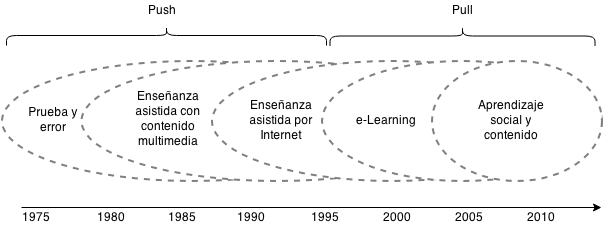
\includegraphics[scale=0.75]{tics/images/tics_history.png}
\caption{Utilización de las \Gls{tic} en la educación desde el año $1975$}
\label{fig:history_tics}
\end{figure}

Para entender la historia de las \Gls{tic} en la educación, se presenta el
gráfico~\ref{fig:history_tics}, en el cual se observa la evolución que sufrió la
utilización de las \Gls{tic} como herramienta en la educación. Se observa que se
parte la historia en cinco corrientes definidas, y a la vez, estas corrientes se
agrupan según el mecanismo de obtención de información, las tres primeras
corrientes se denominan \textit{pull} y las siguientes dos se denominan
\textit{push}. 

\fixme{\textit{Pull} se refiere}{Que es pull? Una corriente? Es la corriente
    pull, los estudian. Obs. Completar la selección} a que los estudiantes
obtenían la información sin participar en la creación de la misma, las
corrientes pedagógicas que marcan tendencias en esta época son el
instruccionismo y el conductismo\cite{white:ict}.

\fixme{\textit{Push} es cuando}{Completar la selección} los alumnos son creados activos de
conocimiento\cite{white:ict,leinonen:ict}, en este periodo de tiempo se
intensifica la creación de herramientas basadas en el constructivismo y el
construccionismo. Es importante notar que las pedagogías de la época
\textit{Pull}, mantienen popularidad y siguen evolucionando, \fixme{solo
    que}{arreglar} a menor medida\cite{white:ict}.

El gráfico~\ref{fig:history_tics} \fixme{muestra}{} el solapamiento entre los diversos
mecanismos utilizados, \fixme{muestra el}{} inicio de la utilización de una herramienta,
pero no su fin, actualmente se sigue utilizando la mayoría de los
enfoques\cite{leinonen:ict}.

Aunque la figura~\ref{fig:history_tics} muestre un progreso lineal de las
corrientes, este progreso no es igual en todo el mundo, y la el grado de
impacto de las \Gls{tic} varia entre países, lo que se conoce como una
\enquote{brecha tecnológica}. \fixme{Las fechas utilizadas en el
    figura~\ref{fig:history_tics} son relacionadas a la evolución en los
    Estados Unidos de Norte America.}{a EE.UU, borrar esto y poner esto en el
    caption}

\observacion{Revisar estructura}
\observacion{Educación, antecedes, instruccionismo?, pero no habla de la
    evolución de instruccionismo, no da a entender en que momento pasa de una a
    otra. Colocar las corrientes en su gráfica 2.1}

\subsection{Instruccionismo}

La educación tradicional o instruccionismo se basa en la transferencia de
conocimiento del profesor al alumno, se enfoca más en el profesor, en la
capacidad del mismo, y en el producto final como resultado de un proceso no
interactivo y bien
documentado\cite{igi:instructionism,johnson2005instructionism}. Los mecanismos
tradicionales para probar la efectividad de este tipo de enseñanza son los
exámenes.

El instruccionismo es conocido además como enseñanza sistemática, enseñanza
explícita, enseñanza directa, y enseñanza activa, siempre enfatizando al
profesor\cite{johnson2005instructionism}.

Epistemológicamente se puede observar al instruccionismo como objetivo, pues
considera que el conocimiento es independiente del entorno, se asume que el
mismo es isomorfo, si el profesor puede enseñar, el alumno puede
aprender\cite{johnson2005instructionism}.

En el instruccionismo, la utilización de las \Gls{tic} en la actualidad se
centra principalmente en mecanismos para proveer contenido, hoy en día se
utilizan plataformas complejas que permiten a los profesores distribuir
contenido y otras actividades relacionadas, estas plataformas se centran bajo
el nombre de \emph{E-Learning}.


\subsubsection{E-Learing} 
\observacion{No se entiende bien la relación entre las corriente pull/push, y
    las corrientes específicas (respecto a su grafo 2.1)}
\observacion{E-Learing, es pull o push. No se refleja bien la relación}

El \emph{E-Learning} se define como la educación y capacitación a través de
medios digitales, incluye todo tipo de medio capaz de distribuir información,
puede ser de en tiempo real como salas de conversaciones y videoconferencias o
puede ser diferido, como por ejemplo foros, enciclopedias. Es particularmente
útil para educación a distancia y con horarios flexibles. Se originó a finales
de la década de $1990$ y tuvo su apogeo a mediados de la década del $2000$,
apoyada por la gran penetración de las \Gls{tic} en la
población\cite{punie:ict}.

Se distribuye contenido masivamente a los alumnos, y luego, de manera discreta
se permite a los mismos colaborar, dejando siempre en claro que primero se debe
asimilar toda la información posible y luego relacionarse con los
demás\cite{leinonen:ict}.


\begin{figure}[h] 
\centering 
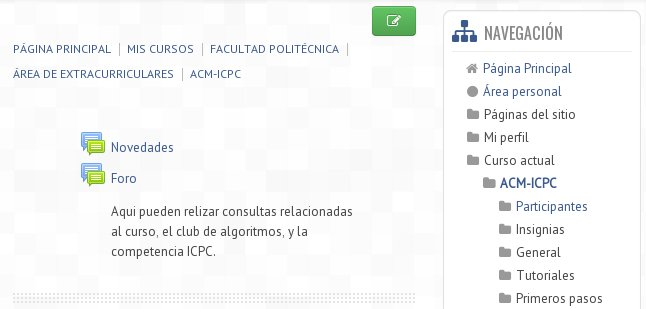
\includegraphics[scale=0.5]{tics/images/moodle.jpg}
\caption{Moodle, plataforma de e Learning} 
\label{fig:moodle}
\end{figure}


La plataforma \emph{Moodle} (ver~\ref{fig:moodle}) cuya primera versión salió en
el $2002$, es una de las principales herramientas del \emph{e-Learning} hoy en
día, permite la creación de cursos específicos por materia y sitios
especializados por instituciones académicas\cite{perkins2006using}. 

La utilización del \emph{e-Learning} tiene varios grados de aplicación en
entornos reales\cite{punie:ict}, que van desde ser simples elementos
complementarios a la clase, como por ejemplo un repositorio para las
diapositivas y otros materiales de clase, hasta cursos completamente en línea,
donde la clase ha sido completamente sustituida.

Sí bien, el \emph{e-Learning} permite la distribución y colaboración en
distintos niveles, no hace un enfoque en el aspecto pedagógico, y se centra en
la forma de transmitir información, y no como la recibe el
alumno\cite{leinonen:ict}, tampoco se centra en la reacción del alumno ante la
información recibida, lo que sí es estudiado por el
conductismo\cite{weegar2012comparison}.

\subsubsection{Conductismo}
\observacion{?}
\observacion{Resumir más, balancer las descripciones}

El conductismo es una corriente de la psicología, creada por \textit{Jhon
    Watson}, y posteriormente perfeccionada por \textit{Pavlov},
\textit{Skinner}, y \textit{Thorndik}. El conductismo defiende la idea de que
todas las acciones que realizan los seres vivos son consecuencia de un
estímulo. Un ejemplo de esta técnica es el experimento de \textit{Pavlov},
\fixme{donde un perro es alimentado cada vez que suena una campana, provocando
    que el perro salive cuando suena la campana, incluso si no existe una
    recompensa (alimento)}{algún mejor ejemplo?}\cite{weegar2012comparison}.

\fixme{El conductismo permite a la epistemología utilizar un enfoque
    científico, permitiendo controlar todas las variables controlables, como el
    estímulo y la reacción, e ignorando los pensamientos y experiencias de las
    personas\cite{weegar2012comparison}. }{Traducir en algo más extendible sin
    usar términos como variables controladas, etc.}

La primera incursión del conductismo con las \Gls{tic}, fue presentada por
\textit{Skinner}, en $1958$\cite{weegar2012comparison}, donde se describe una
máquina que contiene botones y una pantalla donde se presenta una pregunta,
para responder el usuario dispone de varias opciones, cada opción esta
relacionada con un botón, si el aprendiz no presiona el botón correcto, debe
seguir intentando hasta acertar y así avanzar\cite{weegar2012comparison}, este
es el inicio de lo que se conoce como \enquote{Prueba y Error}.

Una característica del conductismo, es la ley de \textit{Thorndike}, indica que
una acción cuya consecuencia es un estímulo favorable, es más probable que sea
repetida\cite{weegar2012comparison}, en la
tabla~\ref{tab:conductismo_estimulo}, se observa los distintos mecanismos 
que propone el conductismo para alentar o desalentar un comportamiento.

\begin{table}[!hbt]
\begin{center}
\begin{tabulary}{\textwidth}{|L|C|C|}
\hline
& Comportamiento alentado & Comportamiento reprimido \\
\hline
Estímulo presente & Refuerzo positivo, por ejemplo, buenas notas & Castigo
Presente, por ejemplo, tiempo después de clase \\
\hline
Estímulo eliminado & Refuerzo negativo, por ejemplo, no hacer quehaceres &
Castigo eliminado, por ejemplo, no permitir utilizar la computadora. \\
\hline
\end{tabulary}
\end{center}
\caption{Tipos de estímulos}
\label{tab:conductismo_estimulo}
\end{table}

A finales de la década de $1970$ e inicios de la década de $1980$,  la
complejidad técnica de las computadoras limitaba la cantidad de herramientas
disponibles, los programas eran desarrollados por profesores, y su objetivo era
que los alumnos puedan poner en práctica lo aprendido en el aula. 


El campo de aplicación de las herramientas, basadas en el experimento de
\textit{Skinner}, se limitaban a matemáticas y lenguaje, donde se podía evaluar
inmediatamente los resultados proveídos por los alumnos, pues, normalmente era
un enunciado y una lista posible de opciones del tipo \enquote{Prueba y
    Error}\cite{leinonen:ict}. 

La cantidad limitada de opciones para responder, provocó que los alumnos no
interpreten los resultados, sino prueben todas las posibles opciones hasta
pasar al siguiente enunciado, sin obtener ningún aprendizaje
significativo\cite{leinonen:ict}.

Cuando aparecieron en el mercado computadoras con multimedia, a finales de la
década de $1980$, la utilización de las \Gls{tic} se simplificaron y dieron
contenido a la posibilidad de incluir contenido multimedia, se argumentó que los
ejercicios de tipo \enquote{Prueba y Error} no cumplieron su objetivo de una
educación profunda por que no contenían multimedia\cite{leinonen:ict}, así, en
se empezaron a distribuir las aplicaciones por \textit{CD-ROM} y contener gran
cantidad de contenido multimedia.

Con la creación de los juegos del tipo \enquote{Prueba y Error} y el contenido
multimedia, se inicio a un nueva corriente denominada \emph{Edutainment},
palabra que representa la unión de la educación y el entretenimiento. 

\subsubsection{Edutainment}
\label{sec:edutainment}

\observacion{Esquema Global
\begin{itemize}
    \item Que es?
    \item Quien creo y cuando?
    \item Ejemplos
    \item Fortalezas y desventajas
\end{itemize}
Tratar de hacer las descripciones más simétricas tirando hacia el resumen}

Los \emph{edutainment} se basan principalmente en el conductismo y el
cognoscitivismo, se enfoca en juegos sencillos que transmiten información simple
al usuario, su estructura se basa en un objetivo claro que está separado de la
experiencia educativa\cite{egenfeldt2007third}. 

Así el \emph{edutainment} pretende agregar entretenimiento a la educación, se
ve al alumno como un receptor pasivo de información que debe asimilarla, y para
aumentar la implicación de los alumnos, el entretenimiento era
agregado\cite{resnick:2004}.

\observacion{Conectar mejor \enquote{Un ejemplo es Math Blaster}}

\emph{Math Blaster} (ver~\ref{fig:math_blaster}) es un \emph{edutainment} donde
el alumno debe responder repetitivamente preguntas aritméticas para obtener
municiones, luego con esas municiones debe completar diferentes misiones en una
nave\cite{bruckman1999can}. Como todas las preguntas se responden mediante un
mecanismo de selección múltiple, y no existe penalización por fallar una
respuesta, los alumnos no reflexionan sobre las respuestas elegidas, seleccionan
una opción aleatoria y si no es la correcta, prueban otra, tras una cantidad
finita de intentos, siempre se obtiene la recompensa deseada.

\begin{figure}[ht!] 
\centering 
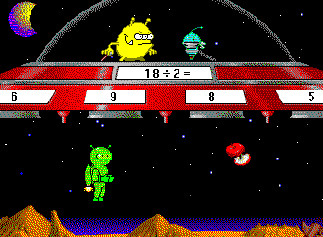
\includegraphics[scale=0.5,natwidth=296,natheight=217]{tics/images/math_blaster.jpg}
\caption{Math Blaster, \emph{edutainment} del año 1987}
\label{fig:math_blaster} 
\end{figure}

\begin{figure}[ht!] 
\centering 
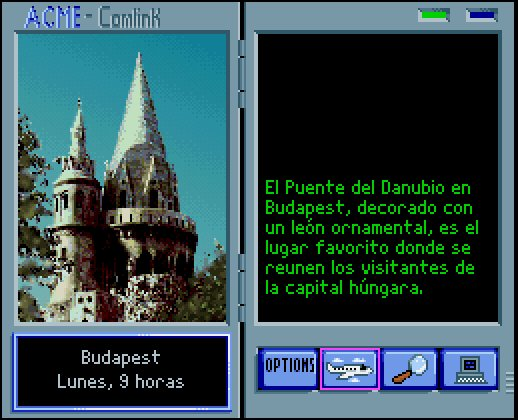
\includegraphics[scale=0.5]{tics/images/carmen.jpg}
\caption{Donde en el mundo esta Carmen Sandiego} 
\label{fig:carmen}
\end{figure}

\enquote{Donde en el mundo esta Carmen Sandiego} (ver~\ref{fig:carmen}) es un
juego que representa el potencial multimedia de esta época, el objetivo del
juego era detener a una serie de criminales mediante varias pistas que eran
provistas en forma de texto. Este exitoso juego demuestra las falencias del
\textit{Edutainment}, siendo visualmente muy atractivo, y con contenido
multimedia acorde a su tiempo, no era más que \enquote{Prueba y Error}, cada
nivel del juego podía ser completado sin leer la información proveída
educativa\cite{charsky:2010}.

Los \emph{edutainment} no logran enseñar habilidades complejas, se enfocan
principalmente en enseñar tareas extremadamente repetitivas que no dependen de
un contexto\cite{charsky:2010,egenfeldt2007third,bruckman1999can}, son
excelentes para enseñar a sumar, pero no para aplicar ese conocimiento, analizar
y obtener conclusiones, o evaluar lo que aprendieron.

Las principales causas por del fracaso de los \emph{edutainment} en su intento
de ser una alternativa viable a la educación son según\cite{egenfeldt2007third}: 

\begin{itemize}

\item \textbf{Falta de motivación interna:} los \emph{edutainment} se centran en
    motivaciones externas, y dejan de lado la motivación interna. Se centran en
    dar recompensas por acciones lo que es una motivación externa, que en que el
    alumno se sienta emocionado al finalizar un nivel, lo que es una forma de
    motivación interna.

\item \textbf{Aprendizaje como anexo:} el principal objetivo del desarrollo de un
    \emph{edutainment} es el de entretener, los objetivos pedagógicos son
    agregados al final. Adicionalmente, este aprendizaje se provee a través de
    largos textos que normalmente son omitidos.

\item \textbf{Interacción limitada:} son construidos con una jugabilidad pobre,
    sin la posibilidad de realizar multiples acciones, normalmente limitados a
    seleccionar respuestas o moverse en un pequeño mundo. 

\item \textbf{Ejercicios de prueba y error sistemáticos:} todas las debilidades
    anteriores se pueden fundamentar en el hecho de que los juegos permiten al
    alumno intentar varias veces sin ser penalizados, además
    de que los alumnos no están motivados, provocaba que todas las opciones sean
    probadas sin el proceso de reflexión necesario para aprender, por ejemplo,
    varios juegos aritméticos solicitaban pruebas del tipo $2+2$ donde el alumno
    probaba diferentes resultados y luego memorizaba el mismo. Se enseñaba a
    probar opciones sin sentido antes que entender y analizar la experiencia.

\end{itemize}

La distribución por medios físicos, aunque contribuyo a la calidad de material
proveído, no resolvió el problema de información actualizada, pues a comienzos
de la década de $1990$, con la popularización de Internet, se genera más
contenido que el que puede ser distribuido por medios físicos, así se accede al
tercer hito de la figura~\ref{fig:history_tics}, donde el contenido es
distribuido por Internet.

La incursión de internet solo permite contenido actualizado, los problemas
persisten y se crean nuevos factores que ensanchan la brecha tecnológica,
ahora, además de poseer una computadora, es necesaria una conexión permanente.
Adicionalmente, la velocidad inicial de Internet no es suficiente para proveer
los mismos entornos ricos en multimedia que sí lo proveían los
CD-ROM\cite{leinonen:ict}.

\textit{Skinner}, se dio cuenta que el compartimiento humano no puede ser
reducido al conductismo, no solo responde a los estímulos, sino, que además
responde a su experiencia previa\cite{weegar2012comparison}, así se estudia el
constructivismo, que se centra en el alumno y sus experiencias.

\subsection{Constructivismo}

El constructivismo es una corriente pedagógica creada por \textit{Jean Piaget}
y \textit{Lev Vygotsky}, cuya idea central es que el aprendizaje humano se
construye, que la mente de las personas elabora nuevos conocimientos a partir
de la base de enseñanzas anteriores. Predica que el aprendizaje de los
estudiantes debe ser activo, deben participar en actividades en lugar de
permanecer de manera pasiva observando lo que se les
explica\cite{hernandez:constructivismo,johnson2005instructionism}.

El constructivismo es un conjunto de prácticas que se enfocan en el alumno,
basados en el contenido, orientados al proceso, interactivos y que responden a
las necesidades e intereses personales de los
alumnos\cite{johnson2005instructionism}.

Se basa en que las personas no entienden, ni utilizan de manera inmediata la
información que se les proporciona, en cambio, el individuo debe
\enquote{construir} su propio conocimiento. El conocimiento se construye a
través de la experiencia y esto conduce a la creación de modelos mentales que
se almacenan en la mente. Estos esquemas van \fixme{cambiando}{}, ampliándose y
volviéndose más \fixme{sofisticados}{Complejo} a través de dos procesos
complementarios: la asimilación y el
alojamiento\cite{hernandez:constructivismo,johnson2005instructionism}.

Epistemológicamente el constructivismo es subjetivo, pues considera que el
conocimiento depende las experiencias\cite{johnson2005instructionism}. 

Las aulas construccionistas crean un mundo realista donde lo más importante es
el aprendizaje el profesor es un facilitator del aprendizaje del
alumno\cite{johnson2005instructionism,nanjappa2003constructing}.

Actualmente, los cursos de \textit{E-Learing}, tradicionalmente conductistas,
están evolucionando para incluir conceptos
constructivistas\cite{weegar2012comparison}, especialmente donde se requiere de
pensamiento de alto nivel\footnote{Del Inglés, \textit{High Order Thinking},
    incluye la capacidad de resolver problemas complejos, y criterios de
    decisión.}, cuya obtención es vista como una estrategia de actividades
necesarias para conseguir objetivos\cite{miri2007purposely}.

Así, las aplicaciones del constructivismo con las \Gls{tic}, es variado,
incluyendo al \textit{E-Learing} y a los \textit{Edutainment}, hasta lo que hoy
se conoce como \textit{Juegos Serios}, los cuales son descritos en el
capítulo~\ref{chap:juegos_serios}. Otros ejemplos de aplicaciones del
constructivismo, son las \textit{wikis}, redes sociales y los
\textit{blogs}\cite{hernandez:constructivismo}.

Las teoría de \enquote{construccionismo} de \textit{Seymourt Papert},
construida sobre el constructivismo, que agrega, entre otras cosas, la
entorno en la que ocurre el aprendizaje\cite{egenfeldt2007third}, permite
explorar más contenido, proveyendo un punto inicial, y permitiendo explorar
posibles soluciones.

\section{Construccionismo y las TIC}

El construccionismo utiliza la tecnología como medio cognitivo  a diferencia de
la educación tradicional que la utiliza para la entrega de contenido. 

El construccionismo es un alternativa prometedora a la educación
tradicional.Desde el punto de vista tecnológico, el contruccionismo es ideal
pues el mismo requiere un alto dinamismo en el traspaso del conocimiento
\cite{sasha:construtivism}. 

El contruccionismo y las \Gls{tic} siempre han estado relacionados, ya que el
mismo se origino con un lenguaje de programación(LOGO)\cite{ict:ttc}. Un
característica importante de esta relación es que tienen la capacidad de
eliminar los problemas de distancia\cite{mariluz:seiousgames}.


\subsection{Historia}

Seymour Papert adoptó el término construccionismo en la década de 1980 para
representar una método pedagógico practicado por John Dewey a principios del
siglo 20. Este método buscaba que la responsabilidad de aprender recaiga en el
estudiante. 

Papert trabajó directamente con el psicólogo evolutivo y filósofo suizo Jean
Piaget, quién elaboro sus teorías de la educación y construcción del
conocimiento al ver e interactuar con los niños. A partir de esta observación
nació el constructivismo según el cual el conocimiento debe ser construido por
el estudiante y los nuevos significados deben ser obtenidos relacionándolos con
significados anteriores por los mismos estudiantes haciendo uso así de sus
propios sistemas de relaciones.

El construccionismo se diferencia de lo anterior en que los estudiantes
construyen las ideas o partes del mundo utilizando herramientas. La elaboración
de representaciones mentales mediante la construcción y el intercambio es la
metáfora del marco contruccionista. 

Durante 1980, Seymor Papert, Wally Feurzeig, Marvin Minsky y John McCarthy y los
miembros del Departamento de Inteligencia Artificial del \Gls{mit} y una
compañía de tecnología en Cambridge, Massachusetts, desarrollaron un nuevo
lenguaje de programación llamado LOGO que tenía por objeto que los estudiantes
construyeran sus modelos en notación LOGO\@. Este juego introduciría de forma
natural las ideas de los procedimientos, funciones, variables, recursividad, la
modularidad, entre otros.

La creación del lenguaje de programación LOGO dio inicio al construccionismo.

Los desarrolladores de LOGO alentaron el uso de la tecnología para la promoción
de nuevas formas de aprendizaje diferentes a las tradicionales. Las comunidades
que adoptaron al contruccionismo con la creación del lenguaje LOGO fueron en su
mayoría aquellas integradas por ingenieros informáticos y matemáticos
\cite{historia:2014}.

\subsection{Bases Pedagógicas}

Para el construccionismo, el conocimiento es construido por el estudiante en
lugar de ser trasmitido por el profesor\cite{moses:2003} y esto sucede
particularmente cuando el mismo se compromete en la elaboración de un producto o
artefacto que tenga un significado y pueda ser compartido\cite{valdivia:sg}. De
esta manera, se permite a los estudiantes elaborar sus propias interpretaciones
razonadas del mundo mediante la interacción con el mismo.

Según Papert, los alumnos estarán mucho más involucrados en su aprendizaje si
construyen artefactos que los demás pueden ver, criticar y tal vez utilizar. Y
además, el alumno se enfrenta a problemas complejos con estas construcciones,
harán el esfuerzo por resolver problemas y aprender ya que la construcción les
motivará\cite{const:vs}.

El enfoque construccionista establece que los seres humanos conocen y aprenden
de formas diferentes por lo tanto, no se puede elaborar una jerarquía de estilos
de aprendizajes\cite{valdivia:sg}.

\subsection{Estado del Arte}

El construccionismo pone énfasis en el \emph{Aprender haciendo}, esta idea
mejora la práctica educativa tradicional o instruccionismo. 

Existen varios emprendimientos o \emph{amigos del contruccionismo}, para la
mayoría de ellos las computadoras son esenciales mientras que para otros el
mayor esfuerzo está en la incorporación de la tecnología en su práctica
educativa~\cite{papertian:const}.

Algunos de estos emprendimientos son:

\begin{description}

\item[Lenguaje de programación LOGO] El lenguaje Logo es la cuna del
	construccionismo, se basa en el principio de que se aprende mejor
	haciendo, pero se aprende todavía mejor si combina la acción con la
	verbalización  y la reflexión acerca de lo que se ha hecho.

\item[Simulación] La simulación de entornos virtuales brinda a los estudiantes
	la posibilidad de experimentar en un entorno controlado, y de esta
	manera les brinda la posibilidad de poner en práctica sus conocimientos
	sin correr riesgos.

\item[Serious Games] Diseñado con el propósito de aprender. Generalmente hace
	uso de la simulación para permitir un aprendizaje más realista.

\item[Lego Serious Play] Es una iniciativa de Lego que busca fomentar el
	pensamiento creativo por medio de la construcción por parte de los
	estudiantes de su identidad y experiencias utilizando legos. 

\item[\Gls{olpc}]. El esfuerzo se centra en dotar a los niños de una computadora
	duradera, accesible y potente en los países en desarrollo, se dice que
	es un descendiente directo del construccionismo. Con esto se busca que
	la computadora personal sea utilizada como un laboratorio intelectual y
	un vehículo para la auto-expresión. OLPC no tiene que ver con la
	escolarización o la escuela, más bien las utiliza como medio de
	distribución de las computadoras a los niños, los cuales pueden
	utilizarlas para aprender en cualquier lugar y momento. Se busca
	fomentar el aprendizaje natural, es decir, aquel aprendizaje sin
	enseñanza\cite{papertian:const}.

\item[Fabricación personal] Neil Gershenfeld, colega de Papert en el Media Lab
	del \Gls{mit} enseñó un curso titulado \emph{Cómo hacer casi cualquier
		cosa}. La idea se centra en la creación de tecnología que se
	necesita para resolver los problemas que se poseen. Papert no sólo
	defendió la idea de que los niños posean computadoras personales, sino
	también que a la larga ellos debían mantenerlas, repararlas e incluso
	construirlas~\cite{papertian:const}.

\end{description}

%http://constructingmodernknowledge.com/cmk08/wp-content/uploads/2012/10/StagerConstructionism2012.pdf

\subsection{Serious Games y Simulación}

\subsubsection{Serious Games}

Un \emph{Serious Game} es un vídeo juego elaborado con el propósito primario que
no es el de entretener\cite{sg:aoverview}, sino tienen una finalidad educativa
explícita y cuidadosamente pensada, utiliza la tecnología y los conceptos de la
industria de los vídeo juegos para encontrar solución a problemas reales. Es
decir, se utilizan para definir los juegos que poseen una pedagogía incrustada,
algún tipo de evaluación ya sea interna o externa y lo que hay que aprender
(contenido) integrado\cite{damien:sg}.

Los \emph{Serious Game} proveen una oportunidad muy importante para enseñar y
desarrollar profesionales, por que ayudan a crear el tipo de educación que los
adultos prefieren, proveen mecanismos para que los estudiantes cometan errores y
experimenten con sus ideas, con su conocimiento y con la teoría en un ambiente
protegido sin riesgos para la vida o la identidad. 

Los beneficios que brindan los \emph{Serious Game} se acentúan en la medida en
la que los mismos proveen entornos más completos en donde realmente se puedan
poner en práctica la teoría, esto ayuda a una comprensión más profunda del área
de interés.

La principal diferencia entre los \emph{Serious Game} y otras aplicaciones de
\emph{E-Learing} es su enfoque en la creación de una experiencia de aprendizaje
significativo, relevante y atractivo. En un \emph{Serious Game} existen metas
claras de aprendizaje pero las mismas se encuentran en un contexto significativo
en donde se deben aplicar los conocimientos y hacer uso de herramientas que
están a disposición para obtener éxito en la resolución de los problemas
presentados. Estos problemas se equilibran a través de la retroalimentación y
otras estrategias para mantener el interés del estudiante. Todo esto hace que en
los \emph{Serious Game} el principal objetivo sea ganar el juego no aprender,
sin embargo sólo se puede hacer esto dominando el aprendizaje
\cite{papertian:const}.

El campo de los \emph{Serious Game} rechaza la idea de que los profesionales de
la educación pueden ser reemplazados fácilmente, para ellos la labor de estos
profesionales es imprescindible para la reflexión y orientación del aprendizaje.
Es cierto que se puede llegar a aprender sin el apoyo de un profesional de la
educación pero se corre el riesgo de perder el enfoque y la eficacia
\cite{elearning:seiousgames}. 

El \emph{serious Game} no se trata de una modelo de aprendizaje pasajero. Varios
autores como Johan Huizinga, Jean Piaget, Wittgenstin y Seymour Papert han
reconocido su importancia  como objeto de aprendizaje. Los juegos deben ser
elaborados teniendo en cuenta el nivel cognitivo del estudiante, es decir, su
etapa de aprendizaje y en que el aprendizaje difiere de acuerdo a la etapa de
vida en la que se encuentre un estudiante. Mediante la práctica repetida de
actividades relacionadas al área de interés se desarrollan habilidades y
destrezas\cite{education:games}. 

Los siguientes son ejemplos de algunas áreas que utilizan Serious Game:

\begin{description}

\item[Militar] Los primeros juegos a menudo se basaban en lucha o combate.
	Durante más de 30 años los juegos han sido reconocidos como herramientas
	factibles en el entrenamiento de militares. En 1996 se creó un juego
	llamado \emph{Marine Doom} en donde la tarea de los jugadores era el
	aprendizaje de formas de ataque, conservación de municiones. Comunicarse
	con eficacia, dar órdenes al equipo de trabajo entre otros. De esta
	manera tuvo lugar una forma de entrenamiento más atractivo, sin el
	costo, dificultad, riesgos e inconvenientes que implicaría el mismo
	entrenamiento en un entorno real. Además se podían crear situaciones que
	en el mundo real serían muy difíciles de
	replicar~\cite{education:games}.

\item[Salud] Este tipo de juegos son cada vez mayores, los juegos de salud se
	utilizan para la formación de profesionales basada en la simulación. En
	2008 el Centro de Simulación Hollier en Birmingham, Reino Unido, realizó
	una prueba que permitió a médicos jóvenes experimentar y entrenar para
	diversos escenarios médicos a través de maniquíes virtuales como
	pacientes, de este modo el aprendizaje se da por la experiencia. En su
	disertación, Roger D. Smith, realizó una comparación entre la enseñanza
	tradicional y la formación mediante realidad virtual y el uso de
	herramientas basadas en la tecnología de juegos en cuanto a la cirugía
	laparoscópica. Como conclusión afirmó que lo último era más barato,
	requería menos tiempo y que permitió menos errores médicos cuando los
	médicos se presentaban en una cirugía real debido a, entre otras cosas,
	la posibilidad de repetición de la experiencia sin riesgo
	alguno~\cite{education:games}.

\item[Juegos corporativos] Este tipo de juegos se han utilizado para la
	selección de personal, la mejora de comunicación entre los directivos y
	su personal de confianza, y la formación de nuevos empleados. Un ejemplo
	de estos juegos es el INNOV8 de IBM que ayuda en el entrenamiento de los
	estudiantes acerca de la gestión de procesos de negocios. Los Serious
	Game pueden ser utilizados incluso para elaborar planes de
	negocios~\cite{education:games}. 

\end{description}

%\cite{sg:aoverview}\cite{houston:sg}\cite{ibm:seriousgames}
%http://ceur-ws.org/Vol-318/Sanchez.pdf
%http://media.futurelab.org.uk/resources/documents/lit_reviews/Serious-Games_Review.pdf

\subsubsection{Simulación}

La simulación se define como el proceso de diseñar un modelo de un sistema real
y, llevar a cabo experimentos con este modelo, con el fin o bien de entender el
comportamiento del sistema o de la evaluación de distintas estrategias para la
operación del sistema\cite{ingalls2008introduction}. 
%[ingalls2008introduction]

Un juego y una simulación podrían llegar a ser muy parecidos, a veces los juegos
tienen motores de simulación, una de las diferencias es que la simulación es muy
dependiente del contexto. 

Existen dos tipos de simulaciones, en primer lugar están las experimentales que
ponen al estudiante en el lugar de un profesional y requieren que el mismo tome
decisiones para alcanzar los objetivos y en segundo lugar están las simbólicas
que buscan que el estudiante deduzca eventos, principios y mejores prácticas
\cite{charsky:2010}. 
%\cite{charsky:2010}

Una simulación esta conformada por:

\begin{description}

\item[Entidades] Son aquellas que cambian el estado de una silumación, estas
	entidades poseen atributos los cuales son sus características
	exclusivas. Por último, una entidad es cualquier objeto que requiera su
	representación explícita. Ejemplo de entidades son: un médico o una
	jeringa en una simulación médica.

\item[Acciones] Las entidades interactúan entre sí a través de acciones. Estas
	acciones puede causar cambios en el estado de la simulación además de
	eventos. Ejemplo de una acción en una simulación médica es la
	esterilización de un instrumento.

\item[Eventos] Los eventos son hechos que ocurren de manera controlada pero no
	siempre predecible en el entorno simulado, los mismos afectan a las
	entidades y deben obligar a realizar alguna de las acciones disponibles
	para tal evento. Ejemplo de un evento en un simulación médica es un paro
	cardíaco del paciente.

\end{description}

La confianza en el modelo o la simulación según\cite{DoDSysEng2001} se establece
mediante:

\begin{description}

\item[La verificación] Es el proceso de determinar si la implementación
	representa con precisión las especificaciones del diseño. 

\item[La validación] Es el proceso de determinar el grado en el que el modelo
	representa de forma exacta la realidad de acuerdo al uso que se tiene
	previsto darle y el nivel de confianza que debe tenerse en la
	evaluación.

\item[La acreditación] Es el proceso de certificación de un modelo para su uso
	con un propósito específico.
%[DoDSysEng2001]

\end{description}

En la actualidad, es cada vez mayor la utilización de la simulación como
herramienta para el entrenamiento ya que los profesores están más familiarizados
con la tecnología. 

Según\cite{humphreys2013developing} los tipos de estudiantes definidos por Kolb
son:

\begin{description}

\item[Accommodating learners] Aprenden de la experiencia e interiorizan el
	aprendizaje a través de experimentación activa. 

\item[Diverging learners] Aprenden a través de experimentación activa, e
	interiorizan el conocimiento reflexionando sobre la experiencia. 

\item[Coverning learners] Aprenden a través del pensamiento abstracto e
	interiorizan el conocimiento a través de la experimentación activa.

\item[Assimilating learners] Aprenden a través del pensamiento abstracto y las
	interiorizan reflexionando sobre las mismas. 
	
\end{description}

Teniendo en cuenta el caso de la enfermería, la misma es una ciencia que atrae a
alumnos del tipo \emph{Diverging learners}, y la simulación es una herramienta
ideal para este tipo de estudiantes.

La mayoría de la literatura encontrada acerca de la simulación y los cuidados de
salud no proporcionan muchos detalles acerca de la implementación de modelos en
áreas amplias, se cree que esto se debe a la complejidad de representar las
actividades relacionas al cuidado de la salud dentro de un modelo de simulación
que debe, de hecho, ser una simplificación de las mismas. Esta simplificación
puede ser un proceso sumamente complejo, por lo cual la mayoría se centra en una
parte de las actividades hospitalarias pero no así en todas. Cuanto mayor sea el
detalle, la simulación conducirá a una representación más realista lo cual
aumenta la confianza en los grupos de interés, sin embargo, más detalle requiere
más datos validados y esto puede ser costoso de obtener\cite{guna:simulation}.

Algunas aplicaciones específicas en el cuidado de la salud son:

\begin{description}

\item[Departamento de emergencia y accidentes] La mayoría de los trabajos
	realizados en esta área se refieren a la optimización de tiempo de
	espera de los pacientes y la organización del personal, de las
	habitaciones,de las ambulancias, para dar mejor atención a los
	pacientes. Un ejemplo de esto es Edsim que que se utiliza para aumentar
	el rendimiento en un departamento de emergencias en EE.UU como parte de
	un sistema que permite el desvío de ambulancias en los períodos pico de
	demanda, el cual incluye la introducción de salones de descarga y la
	disminución del tiempo de estancia\cite{guna:simulation}. 
	
\item[Instalaciones para pacientes hospitalizados] Los trabajos se centran en la
	mejora en la atención con respecto al flujo de pacientes así como la
	ocupación de camas. Muchos trabajos tratan de demostrar como se podrían
	utilizar modelos matemáticos para esto. Harper y Shahani presentaron un
	modelo de simulación flexible relacionado a estás cuestiones de
	pacientes hospitalizados, el mismo utiliza TOCHSIM, flexible en el
	sentido de que aborda también problemas como la creación de una nueva
	unidad en el hospital\cite{guna:simulation}.

\item[Clínicas para pacientes ambulatorios] En este sentido la simulación se
	utiliza para minimizar el tiempo de espera de los pacientes en clínicas
	externas, es decir, aquellas en las que se sacan citas. El tiempo de
	espera no sólo implica la espera dentro de la clínica sino también el
	tiempo que pasa entre el momento en el que se solicita un cita y el día
	de la cita. Un ejemplo de esto es CLINSIM que se utilizó en el Reino
	Unido para observar como la política de operación puede influir en los
	tiempos de espera de los pacientes\cite{guna:simulation}. 

\item[Formación medica y quirúrgica] Se centran en tareas específicas y en la
	formación de un conjunto limitado de habilidades referentes a estas
	tareas. Los ejemplos más recientes son entrenamiento para un intubación
	esofágica, capacitación y evaluación de capacidades laparoscópicas,
	entrenamiento para la palpación de tumores de mama\cite{mantovani:vr}. 

\item[Sistemas de formación de emergencias] Se refieren a aquellas simulaciones
	diseñadas para la rápida respuesta médica. Incluye desde pacientes
	virtuales dinámicos cuya acción por parte del estudiante produce un
	cambio clínico en el mismo y una respuesta al estudiante.  Otro ejemplo
	es el utilizado en la marina de EE.UU que intenta formar a los
	profesionales para su rápida acción frente a desastres civiles y donde
	la estabilización de pacientes se tenga que dar con recursos
	limitados~\cite{mantovani:vr}. 

\item[Entrenamiento para profesionales de salud mental] Janssen LP creó una
	simulación para educar a los psiquiatras y profesionales de la salud en
	lo que es tener esquizofrenia llamada \emph{el viaje en autobús} que
	trata de mostrar lo que pasa dentro de de la mente de una persona con
	esquizofrenia cuando viaja en autobús en base a experiencias relatadas
	por pacientes y médicos\cite{mantovani:vr}. 

\end{description}


\section{Ventajas y desafíos}
\label{sec:tics_ventajas}

Durante la historia de las \Gls{tic} en la educación, se han encontrado
diferentes dificultades a la hora de aplicar los nuevos conceptos en la
educación, desde los primeros enfoques que carecían de bases pedagógicas válidas
hasta la actualidad, el principal problema es falta de motivación de los
profesionales de la educación para emplear las
\Gls{tic}\cite{punie:ict,ict:romeo}.

%\todox{Reconsiderar el párrafo que esta comentado bajo este todo}
%\fixme{El contenido proveído actualmente puede ser considerado como un conjunto
%    de buenas prácticas\cite{punie:ict} y así, omiten completa o parcialmente el
%    contexto donde esa buena práctica fue generado. }{No se entiende de donde
%    sale esto, de que habla y para qué?}

Aún así, las \Gls{tic} han tenido un impacto positivo en la educación, pero el
mismo no es el esperado\cite{punie:ict}, por ejemplo, iniciativas como el
\emph{edutainment} que prometían ser la solución a los problemas
educacionales no cumplieron las expectativas.

Sucesivos fracasos en los resultados obtenidos dotaron a los \emph{edutainment}
de una reputación negativa, y hoy en día son considerados como un método educativo 
ineficiente, pues son un ejercicio de \emph{prueba-error} ocultos bajo un juego poco 
entretenido, además de su incapacidad de enseñar como aplicar conceptos aprendidos 
a un entorno real\cite{resnick:2004}.

Mientras que la utilización de las \Gls{tic} puede eliminar problemas actuales
como el aislamiento y la falta de pensamiento de alto nivel\cite{punie:ict}, la
brecha social existente implica otro riesgo para la utilización de las \Gls{tic}
en la educación, aquellos que no posean los recursos económicos necesarios para
acceder a la misma no se verán beneficiados por las \Gls{tic}\cite{punie:ict}.

Las empresas involucradas en el área de las \Gls{tic} en
educación siguen en la época donde los juegos son prueba y error, esto no
significa que los mismos no funcionen, sino que pueden ser mejorados
considerablemente\cite{egenfeldt2007third}.

Otro de los desafíos actuales es la dificultad comercial impuesta por la
historia de los mismos, es muy difícil para los juegos actuales presentar
promesas realistas, principalmente por el antecedente sentado por los
\emph{edutainment}\cite{egenfeldt2007third}

Las principales ventajas de la utilización de las \Gls{tic} en la educación son:

\begin{itemize}

\item \textbf{Nuevos modelos pedagógicos:} teorías como el constructivismo moderno
    enfatizan el proceso de como adquirir (aprendizaje) conocimiento y no
    solamente como transmitir el conocimiento en sí
    (enseñanza)\cite{guenaga2013serious}.

\item \textbf{Eliminación de distancias:} Con la aparición de las computadoras y los
    satélites,  el mundo se ha convertido en una aldea global, y las distancias
    en cuestiones de transmisión de información se han vuelto
    insignificantes\cite{mohammed2013information},  los medios tradicionales
    como bibliotecas, o escuelas están limitados a un espacio  físico, con el
    uso de las \Gls{tic}, esta restricción física desaparece\cite{tinio:ict}.

\item \textbf{Colaboración distribuida:} como consecuencia del punto anterior, los
    alumnos pueden colaborar de manera más sencilla pues no tienen limitaciones
    físicas. Además, los alumnos pueden consultar con expertos que están en
    linea, e incluso tener mentores en linea, estas tutorías pueden ser uno a
    uno, por ejemplo mediante comunicaciones por correo electrónico. Además
    permite la colaboración masiva entre estudiantes de intereses comunes,
    mediante foros y redes sociales\cite{unesco:ict}.

\item \textbf{Motivación para aprender:} Las \Gls{tic} tienen un impacto positivo en el
    proceso de aprendizaje especialmente en lo referente al compromiso
    con\cite{passey2004motivational,egenfeldt2007third}:
	    
    \begin{itemize}
    \item \textbf{La actividad}: a través de estímulos visuales, auditivos, etc.
    \item \textbf{La capacidad de investigación}: es más fácil acceder a gran cantidad de
        información bibliográfica.
    \item \textbf{La capacidad de escritura y lectura}: emitiendo compartir  ideas de
        manera más legible y mejorarlas iterativamente.
    \item \textbf{La capacidad de presentación}: es más fácil presentar trabajos
        profesionalmente a un público mayor.
    \end{itemize}
	    
\item \textbf{Adquisición de habilidades básicas:} las habilidades necesarias para
    utilizar de manera efectiva las \Gls{tic} se están convirtiendo en una
    necesidad básica, un aprendizaje guiado por las mismas puede ayudar a una
    rápida asimilación de los conceptos relacionados.

\end{itemize}

Uno de los desafíos más importantes que enfrentan las \Gls{tic} para convertirse
en una alternativa viable es la inversión en infraestructura
necesaria\cite{unesco:ict}.




% Nueva organización
% 
%  Introducción
%  Evolución
%   Antecedentes
%   Instruccionismo
%   Behaviourism
%   Constructivismo
% Construccionismo
% Ventajas y desafíos

%\chapter{Juegos serios}
\label{chap:juegos_serios}

Un \emph{Juego Serio} es \enquote{Un juego que posee un propósito educacional
    explícito y bien elaborado, y cuya intención no es la de únicamente
    entretener} según la definición de \emph{Clark Abt} en su libro
\emph{Serious Games} \cite{abt1987serious}, a esta definición hay que agregar el
involucramiento del usuario en el juego, característica importante de los juegos
serios, además, de ser lo que los diferencia de un
\emph{Edutainment}\cite{resnick:2004,charsky:2010}. Otras definiciones que
permiten entender mejor qué es un juego serio son:

\begin{itemize}
    \item Es una aplicación desarrollada con conceptos de videojuegos (lo que
        incluye la tecnología y los principios de diseño), teniendo como
        principal objetivo el entrenamiento o la educación al mismo tiempo que
        el entretenimiento\cite{ludus:sg}.
    \item Son videojuegos que involucran y entretienen a sus usuarios en la
        búsqueda de un determinado propósito que no es el de puro
        entretenimiento\cite{ludus:sg}.
    \item Son los videojuegos que poseen pedagogía incluida, además de algún tipo de
        evaluación, ya sea interna o externa, y el contenido que se desea
        enseñar\cite{damien:sg,sg:aoverview}.
        
    \item Videojuegos que involucran al usuario con la actividad, y contribuyen al logro de un propósito definido que no es el de entretener\cite{sg:aoverview}.
\end{itemize}

Teniendo en cuenta estas definiciones, se considera a un juego serio como
\emph{Un videojuego que posee un propósito educacional explícito, cuyo objetivo
    principal es el de educar y utiliza conceptos lúdicos para involucrar y
    entretener al usuario}. 

En este capítulo, para un mejor entendimiento de lo que es un juego serio, se
describen sus características, ventajas y desafíos. Luego se presenta un modelo
de desarrollo que fue utilizado en un juego serio denominado \textit{Living
    Forest}. Por último, se describe la actualidad de los juegos serios,
incluyendo las áreas de aplicación, las principales conferencias y ejemplos de
desarrollos recientes. 

\section{Características}

Los \emph{Serious Game} proveen una oportunidad muy importante para ayudar en la
enseñanza y desarrollo de profesionales, por que ayudan a crear el tipo de
educación que los adultos prefieren, proveen mecanismos para que los estudiantes
cometan errores y experimenten con sus ideas, con su conocimiento y con la
teoría en un ambiente protegido sin riesgos para la vida o la identidad. 

Los beneficios que brindan los \emph{Serious Game} se acentúan en la medida en
la que los mismos proveen entornos más completos en donde realmente se puedan
poner en práctica la teoría, esto ayuda a una comprensión más profunda del área
de interés.

La principal diferencia entre los \emph{Serious Game} y otras aplicaciones de
\emph{E-Learing} es su enfoque en la creación de una experiencia de aprendizaje
significativo, relevante y atractivo. En un \emph{Serious Game} existen metas
claras de aprendizaje pero las mismas se encuentran en un contexto significativo
en donde se deben aplicar los conocimientos y hacer uso de herramientas que
están a disposición para obtener éxito en la resolución de los problemas
presentados. Estos problemas se equilibran a través de la retroalimentación y
otras estrategias para mantener el interés del estudiante\cite{papertian:const}.

El campo de los \emph{Serious Game} rechaza la idea de que los profesionales de
la educación pueden ser reemplazados fácilmente, para ellos la labor de estos
profesionales es imprescindible para la reflexión y orientación del aprendizaje.
Es cierto que se puede llegar a aprender sin el apoyo de un profesional de la
educación pero se corre el riesgo de perder el enfoque y la eficacia
\cite{elearning:seiousgames}. 

El \emph{serious Game} no se trata de una modelo de aprendizaje pasajero. Varios
autores como \emph{Johan Huizinga}, \emph{Jean Piaget}, \emph{Wittgenstin} y
\emph{Seymour Papert} han reconocido su importancia como objeto de aprendizaje.
Los juegos deben ser elaborados teniendo en cuenta el nivel cognitivo del
estudiante, es decir, su etapa de aprendizaje y en que el aprendizaje difiere de
acuerdo a la etapa de vida en la que se encuentre un estudiante. Mediante la
práctica repetida de actividades relacionadas al área de interés se desarrollan
habilidades y destrezas\cite{education:games}.

\subsection{Ventajas}


Las \Gls{tic} y los juegos serios en particular son herramientas de inestimable
valor para apoyar los nuevos procesos de enseñanza-aprendizaje y
evaluación\cite{guenaga2013serious}.

Los juegos serios, constituyen un escenario privilegiado para el desarrollo de
todos los componentes de las competencias (conceptos, habilidades, actitudes,
motivaciones, valores, etc.) ya que permiten desarrollar vivencias en las que
ponerlos en práctica, permitiendo el entrenamiento en situaciones que en muchas
ocasiones son similares a las que se encuentran en entornos
reales\cite{guenaga2013serious}.

Además, favorecen la autoestima y tienen un factor motivacional, así como la
posibilidad de desarrollar destrezas y estrategias cognitivas como la capacidad
de resolución de problemas, toma de decisiones, búsqueda y organización de la
información, habilidades perceptivo-motrices y razonamiento
abstracto\cite{guenaga2013serious}.

Se puede añadir también que aumentan la capacidad de coordinación, percepción
espacial y ampliación del campo visual, lo que tiene una incidencia en la
lectura y el manejo eficiente en ambientes 3D\cite{guenaga2013serious}. 

Más allá del logro de competencias puntuales, las teorías modernas de
aprendizaje sugieren que el aprendizaje es más efectivo cuando es activo,
experiencial, situado, basado en problemas y se recibe retroalimentación
inmediata y los juegos basado en aprendizaje se fundamentan en esos
principios\cite{guenaga2013serious}.



\subsection{Desafíos}


El potencial de un juego serio no es ilimitado, los desarrolladores se
encuentran con múltiples desafíos que deben ser superados para poder obtener un
juego serio que obtenga las ventajas citadas previamente y pueda ser de utilidad
en la educación formal.

Un juego serio, como el resto de la \textit{media}, no puede cambiar el
comportamiento de una persona por sí solo, un juego acerca de hábitos
saludables, no hará del jugador un nutricionista, pero si permiten al jugador
explorar las opciones, tener en cuenta las consecuencias de sus actos y poner en
práctica su conocimiento\cite{education:games}, adicionalmente es importante
definir lo que forma parte del juego serio y lo que no, pues un juego serio no
debe incluir todas las características de la
realidad\cite{stapleton2004serious,videojuegos:gonzaleztardon}. 

La forma tradicional de evaluación presenta dificultades a los juegos serios,
por ejemplo, las pruebas tradicionales contienen un grupo de preguntas, las
cuales son vistas de manera independiente, en cambio en un juego serio, las
acciones son dependientes del contexto y las acciones previamente
realizadas\cite{shute2009melding}.

En cuanto al objeto pedagógico, el área en la cual se utiliza un juego serio es
un factor determinante para el éxito del mismo, es decir, se debe responder a la
pregunta: \emph{¿Es necesaria una solución basada en juegos
    serios?}\cite{stapleton2004serious}, las áreas de aplicación de un juego
serio se describen con más detalle en~\ref{sec:areas_aplicacion}.

Uno de los factores más complicados a la hora del desarrollo de juegos serios es
la limitación de recursos financieros, esto no quiere decir que no existan
recursos para su desarrollo, sino que, comparados con los recursos invertidos en
otras \textit{media} es insignificante\cite{stapleton2004serious}. Como
consecuencia de las limitaciones financieras, los desarrolladores no siempre
pueden acceder a tecnología de última generación\cite{stapleton2004serious}

\section{Aplicaciones}

Los siguientes son ejemplos de algunas áreas que utilizan \textit{Serious Game}
\todox{Arreglar esta introducción}


\subsection{Militar}

Los primeros juegos a menudo se basaban en lucha o combate.
Durante más de 30 años los juegos han sido reconocidos como herramientas
factibles en el entrenamiento de militares. En 1996 fue lanzado un juego
llamado \emph{Marine Doom} en donde la tarea de los jugadores era el
aprendizaje de formas de ataque, conservación de municiones, comunicarse
con eficacia, dar órdenes al equipo de trabajo entre otros. De esta
manera tuvo lugar una forma de entrenamiento más atractivo, sin el
costo, dificultad, riesgos e inconvenientes que implicaría el mismo
entrenamiento en un entorno real. Además se podían crear situaciones que
en el mundo real serían muy difíciles de replicar y donde los errores
pueden ser catastróficos además, permite la repetición hasta alcanzar la
maestría\cite{education:games}.

\subsection{Salud}

Este tipo de juegos son cada vez mayores, los juegos de salud se
utilizan para la formación de profesionales basada en la simulación. En
2008 el Centro de Simulación Hollier en Birmingham, Reino Unido, realizó
una prueba que permitió a médicos jóvenes experimentar y entrenar para
diversos escenarios médicos a través de maniquíes virtuales como
pacientes, de este modo el aprendizaje se da por la experiencia. En su
disertación, Roger D. Smith, realizó una comparación entre la enseñanza
tradicional y la formación mediante realidad virtual y el uso de
herramientas basadas en la tecnología de juegos en cuanto a la cirugía
laparoscópica. Como conclusión afirmó que lo último era más barato,
requería menos tiempo y que permitió menos errores médicos cuando los
médicos se presentaban en una cirugía real debido a, entre otras cosas,
la posibilidad de repetición de la experiencia sin riesgo
alguno\cite{education:games}.


\subsection{Juegos corporativos}

Este tipo de juegos se han utilizado para la
selección de personal, la mejora de comunicación entre los directivos y
su personal de confianza, y la formación de nuevos empleados. Un ejemplo
de estos juegos es el INNOV8 de IBM que ayuda en el entrenamiento de los
estudiantes acerca de la gestión de procesos de negocios. Los Serious
Game pueden ser utilizados incluso para elaborar planes de
negocios\cite{education:games}. 


\section{Corrientes relacionadas}

Los juegos serios son el solapamiento de tres corrientes, los videojuegos, las
técnicas de enseñanza y la simulación educativa\cite{education:games}, tal y
como se observa en la figura~\ref{fig:corrientes_relacionadas}. 

\begin{figure}[ht]
\centering
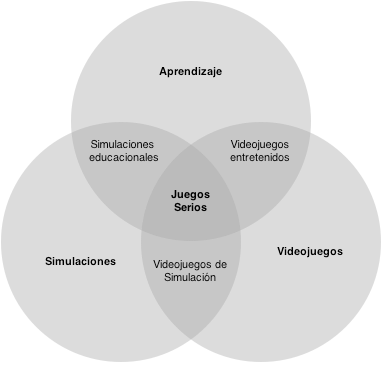
\includegraphics[scale=0.7]{juegos_serios/corrientes_paralelas.png}
\caption{Ubicación de los juegos serios entre los videojuegos, la simulación y
    la educación}
\label{fig:corrientes_relacionadas}
\end{figure}

Cuando se utilizan aspectos de videojuegos con simulaciones, se obtienen videojuegos,
cuyo objetivo es entretener mientras son similares a la realidad, dentro de esta
categoría podemos encontrar juegos como \emph{Gran Turismo}; sí mezclamos
factores relacionados al aprendizaje y a las simulaciones se obtienen
simulaciones sin interacción con el usuario que buscan mostrar o enseñar como se
comportan distintos fenómenos físicos, sociales, etc.

Los \emph{Edutainment} pueden ser vistos como los predecesores de los juegos
serios, los mismos son descritos en~\ref{sec:edutainment}.

\subsection{Simulaciones educativas}


La simulación se define como el proceso de diseñar un modelo de un sistema real
y, llevar a cabo experimentos con este modelo, con el fin o bien de entender el
comportamiento del sistema o de la evaluación de distintas estrategias para la
operación del sistema\cite{ingalls2008introduction}. 

Aunque un juego serio y una simulación pueden parecer muy similares, se
diferencian en que, si bien muchos videojuegos incluyen una simulación, una
simulación no utiliza características típicas de los videojuegos como la fantasía,
puntuación, etc\cite{sg:aoverview}.

La simulación en el ámbito de la educación evolucionó desde simples motores de
reglas hasta complejos entornos. La simulación demostró ser una herramienta muy
útil en el ámbito laboral\cite{mariluz:seiousgames}, pues enseña al usuario a
encarar situaciones muy difíciles de representar en entornos completamente
controlados y provee mecanismos para comprobar la efectividad de la herramienta. 

Actualmente la simulación se utiliza más en el ámbito empresarial pues las
empresas son las más necesitadas de innovar en el ámbito de la enseñanza. Un
ejemplo de esta necesidad se da, por ejemplo, en el entrenamiento de nuevos
vendedores, es muy difícil enseñar a un vendedor como debe vender los productos
con un pizarrón y/o una presentación, en cambio la simulación permite que el
mismo pueda probar cosas nuevas y experiencias de sus compañeros (o instructor),
convirtiendo así el aprendizaje en colectivo\cite{mariluz:seiousgames}.

Existen dos tipos de simulaciones, en primer lugar están las experimentales que
ponen al estudiante en el lugar de un profesional y requieren que el mismo tome
decisiones para alcanzar los objetivos y en segundo lugar están las simbólicas
que buscan que el estudiante deduzca eventos, principios y mejores
prácticas\cite{charsky:2010}. 


\subsection{Diferencia entre juegos serios, simulaciones y los Edutainment}

Estos tres entornos virtuales altamente interactivos, poseen posibilidades y
fines distintos, pueden parecer similares pero poseen las siguientes
diferencias\cite{education:games}:

\begin{itemize}
\item \textbf{Simulaciones educativas}: utilizan escenarios rigurosamente
    estructurados con un conjunto altamente refinado de normas, retos y
    estrategias que son cuidadosamente diseñados para desarrollar las
    competencias específicas que se pueden transferir directamente al mundo
    real.
\item \textbf{Videojuegos:} son actividades atractivas y divertidas que
    habitualmente se utilizan exclusivamente para el entrenamiento pero también
    permiten una exposición con un conjunto determinado de herramientas,
    argumentos o ideas. Todas las partidas se juegan en un mundo estructurado
    por normas específicas, mecanismos de retroalimentación, y las herramientas
    necesarias, aunque no están tan definidas como en las simulaciones.
\item \textbf{Edutainment:} son aplicaciones educativas cuyo principal propósito
    es el de entretener, y el aprendizajes es un añadido. Los
    \emph{edutainment}, se centran en la motivación externa.
\end{itemize}

\section{Desarrollo de juegos serios}
\label{sec:desarrollo}

Una vez definido lo que es un juego serio, queda la tarea de definir cómo
realizar uno, incluyendo qué factores deben ser tomados en cuenta durante su desarrollo.
% Esto hacemos/ esto de los problema comunes? wtf no me acuerdo de haber leido nunca esto

Según~\cite{education:games} un juego serio debe cumplir los siguientes
tres criterios:

\begin{itemize}

\item \textbf{Implementación técnica}: se refiere a la actividad de programación
    y ejecución de un patrón de diseño. Incluye la perfecta integración de los
    elementos de diseño en el videojuego. 

\item \textbf{Adecuación para la educación:} la capacidad del videojuego para hacer
    frente a las metas curriculares o educativas y la habilidad o el
    conocimiento del jugador relativo a los contenidos educativos que se aborde.

\item \textbf{Integración total con los objetivos pedagógicos:} la integración
    del patrón de diseño y el videojuego en general con los objetivos
    educativos.

\end{itemize}


Adicionalmente, el diseño del mismo se tiene que centrar en cuatro factores o
dimensiones, las cuales son\cite{education:games}:

\begin{itemize}
\item \textbf{Contexto:} es decir, donde ocurre el aprendizaje, lo que va desde
    aspectos macro, como  factores políticos, económicos e históricos, hasta
    aspectos micro como la experiencia y  antecedentes de los profesores, costos
    de licencia, entre otros.
\item \textbf{Tipo de aprendizaje:} para el individuo o grupo, requiere que se
    considere su  estilo de aprendizaje y sus conocimientos previos, y qué
    métodos se ajustan mejor a sus  necesidades.
\item \textbf{Modo de representación:} lo que incluye el nivel de interactividad
    requerido, la fidelidad y  el nivel de inmersión producido. Además cubre la
    narración de los hechos, la separación de los  aspectos de inmersión con la
    reflexión de haber utilizado el videojuego. Y de manera importante  enfatiza
    el potencial de retroalimentación que refuerza el aprendizaje.
\item \textbf{Principios pedagógicos:} es necesario reflexionar sobre los
    modelos de aprendizaje lo  que permite producir apropiados planes de
    lecciones.
\end{itemize}

Estas dimensiones no pueden ser consideradas individualmente, todas están
relacionadas  como se muestra en el figura~\ref{fig:desarrollo_dimensiones}.

\begin{figure}[H]
\centering
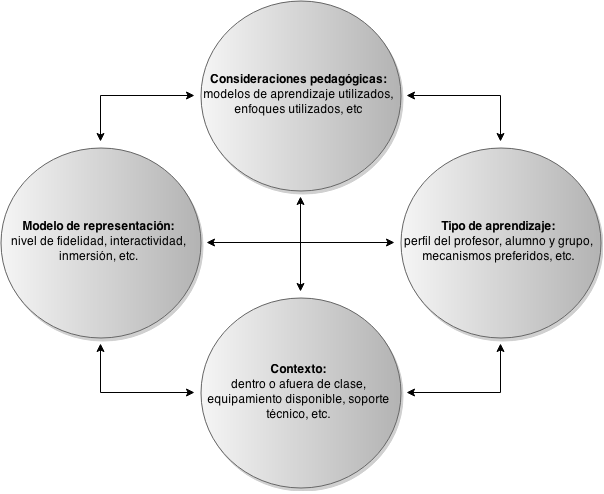
\includegraphics[scale=0.5]{juegos_serios/desarrollo_dimensiones.png}
\caption{Relación entre las cuatro dimensiones a considerarse en un videojuego
    basado en aprendizaje}
\label{fig:desarrollo_dimensiones}
\end{figure}

A continuación se da un ejemplo de flujo de diseño para implementar un juego serio 
manteniendo todas sus características incluyendo los criterios y factores descritos 
anteriormente.

\subsection{Flujo de diseño de un juego serio}

\textit{Pereira}\cite{pereira2009design} en el diseño del videojuego \emph{Living
    Forest} utiliza un conjunto de pasos bien definidos como modelo de creación
de un juego serio a partir de la definición previa de las competencias básicas
que se desean enseñar.

Es importante notar que este modelo se adecua a las dimensiones y criterios
definidos previamente. La obtención de las competencias básicas no forma parte
de este flujo pues, se asume que es un paso previo al diseño.

\begin{figure}[ht!]
\centering
\begin{tikzpicture}[auto]
    % Place nodes
    \node [block] (1) {1. Objetivos de diseño};
    \node [block, right of=1, node distance=5cm] (2) {2. Competencias básicas relacionadas con la educación};
    \node [block, right of=2, node distance=5cm] (3) {3. Investigación del dominio};
    \node [block, below of=3, node distance=3cm] (4) {4. Diseño del juego};
    \node [block, left of=4, node distance=5cm] (5) {5. Tiempo en el juego};
    \node [block, left of=5, node distance=5cm] (6) {6. Acciones de jugabilidad};
    \node [block, below of=6, node distance=3cm] (7) {7. Indicadores};
    \node [block, right of=7, node distance=5cm] (8) {8. Representación e interacción};
    \node [block, right of=8, node distance=5cm] (9) {9. Implementación};
    \node [block, below of=9, node distance=3cm] (10) {10. Evaluación};
    % Draw edges
    \path [line] (1) -- (2);
    \path [line] (2) -- (3);
    \path [line] (3) -- (4);
    \path [line] (4) -- (5);
    \path [line] (5) -- (6);
    \path [line] (6) -- (7);
    \path [line] (7) -- (8);
    \path [line] (8) -- (9);
    \path [line] (9) -- (10);
\end{tikzpicture}
\caption{Flujo de diseño propuesto de un juego serio}
\label{fig:tics_flujo_diseño_prop}
\end{figure}

Teniendo las competencias básicas que se desea sean enseñadas, practicadas o
perfeccionadas por el usuario mientras utiliza el juego serio a diseñar, los
siguientes puntos que deben ser diseñados son
(ver~\ref{fig:tics_flujo_diseño_prop}):

\begin{enumerate}
\item \textbf{Objetivos de diseño:} definen cuál es el propósito del videojuego, donde
    se toman en cuenta los objetivos pedagógicos, así como también objetivos que
    garanticen que el mismo sea agradable, intuitivo y motivador.

\item \textbf{Competencias básicas relacionadas con la educación:} se identifican
    aquellas que influyen en el diseño del videojuego, se definen los conocimientos
    mínimos que se desea que tenga un usuario que lo utilice.

Las competencias básicas pueden tener diferentes orígenes, en el ámbito
académico se puede utilizar el plan de estudios, en una empresa se pueden
utilizar los objetivos y la visión de la misma.

\item \textbf{Investigación del dominio:} esta fase se encarga de recabar
    información exacta acerca del dominio en el cual se desenvuelve el juego
    serio, en esta fase es importante que participe un experto en el dominio,
    por ejemplo, en el ámbito académico se puede contar con un profesor experto
    en el dominio.

Es importante realizar la pregunta \emph{¿Qué nivel de detalle es necesario?},
para así definir qué contenido incluir, y qué factores se deben analizar.

Además es necesario investigar las acciones que se podrían realizar dentro del
videojuego, cómo se desenvolverá el jugador, por cada acción definida, se deben
analizar los elementos y factores relacionados que se deben modelar.

\item \textbf{Diseño del juego:} a partir de la idea original y basado en la
    información recogida se determina el papel desempeñado por el jugador (de
    acuerdo a la semántica y pragmática de las acciones y decisiones que está
    llamado a hacer). 

Se define el nivel de aproximación a la realidad, el nivel de detalle del
entorno, del jugador y de las acciones.

Otro factor que se debe tener en cuenta en esta fase es la cantidad de tiempo
que pasará un jugador en el juego, se deben modelar todas las acciones del
jugador y el entorno de acuerdo a este tiempo.

\item \textbf{Tiempo de juego:} el primer factor que se debe estudiar es el
    período de adaptación del jugador, lo que depende de la intuitividad del
    videojuego, este tiempo debe ser analizado por separado a la hora de realizar un
    análisis de los resultados.
    
    Se debe definir la duración de las partidas y la forma en la que 
    se mostrarán los resultados de las acciones.
% Esto es jodido por que no hicimos, osea mmm no se
%Si el videojuego tiene una duración reducida, se tienen que analizar mecanismos %para
%mostrar los resultados de las decisiones a largo plazo, además de como mostrar
%los resultados de las acciones de corto plazo.

\item \textbf{Indicadores:} es todo aquello que muestre información relevante al
    jugador acerca de su estado, ejemplos de este tipo de indicadores son el
    puntaje, tiempo empleado, objetivos cumplidos. 

La definición de como se juzgará la calidad de una partida del jugador debe ser
definida, normalmente mediante un puntaje general, el mismo debe mostrar
claramente los resultados de las acciones, si las mismas fueron positivas o
negativas para el logro final de los objetivos.

\item \textbf{Representación e interacción:} representación se refiere a como se
    visualiza el entorno, e interacción a como se relaciona el jugador con su
    entorno.

Se inicia con un bosquejo de las representaciones de la escena del videojuego, para
así poder definir los elementos que forman parte de la escena.

Otros bosquejos necesarios son los del concepto que se modela en la lógica del
videojuego, para así definir las animaciones del entorno y del jugador.

Se deben definir las alertas sonaras, qué partes del entorno produce sonidos,
cómo el jugador recibe estas alertas (por ejemplo si el origen de las mismas es
siempre el mismo o importa la distancia a la cámara), se puede agregar música de
ambiente si el videojuego lo amerita.

Se define la interfaz del usuario, qué información será representada, las
acciones disponibles desde la misma, además se define si el mismo será en
primera persona (la cámara son los ojos del jugador) o en tercera persona (la
cámara se sitúa inmediatamente atrás y arriba de la cabeza), como será la
interacción con la cámara, acercamientos y movimientos para contemplar el
entorno.

\item \textbf{Implementación:} en esta etapa se estudia el estado del arte de las
    plataformas tecnológicas disponibles para el desarrollo del videojuego, se toman
    en cuenta los factores como la disponibilidad de componentes, de
    documentación, lenguajes de programación y herramientas de pruebas
    automáticas.

El proceso puede ser iterativo, entre sesiones de implementación y evaluación de
lo implementado, para así poder realizar optimizaciones enfocadas especialmente
en la estética, la retroalimentación y el estado del jugador.

\item \textbf{Evaluación:} durante el desarrollo del juego serio, se deben
    realizar varias sesiones de evaluación, por ejemplo, con los responsables o
    expertos y miembros de la audiencia objetivo. Así mismo, se deben realizar
    evaluaciones con los grupos de interés las cuales se centran en la adaptación
    del videojuego (usabilidad). 

La primera evaluación mencionada se centra en la validación del modelo de la simulación
(refinamiento), mientras que la segunda evaluación sirve para probar el videojuego en
un escenario (parecido al final) y evaluar los aspectos relacionados con el
proceso de aprendizaje.  

\end{enumerate}

\section[Ejemplos]{Ejemplos de juegos serios}

En este apartado se darán detalles de varios casos de éxito de aplicaciones que
tienen como objetivo ayudar en el aprendizaje del usuario o jugador en algún
tema en particular.

Se presentan varios casos de éxito, donde se puede ver cómo la utilización de
las \Gls{tic} provocaron un resultado positivo en las personas que lo
utilizaron.

\subsubsection{Triage Trainer}

\begin{itemize}
\item \textbf{Tipo:} Simulación de entrenamiento.
\item \textbf{Destinatarios:} Médicos, enfermeros, paramédicos y otros
    rescatistas.
\item \textbf{Contenido:} Entrenamiento para evaluar a los pacientes en un lugar de
  emergencia.
\item \textbf{Desarrollador:} \emph{TruSim}.
\end{itemize}

\begin{figure}[ht!] 
\centering 
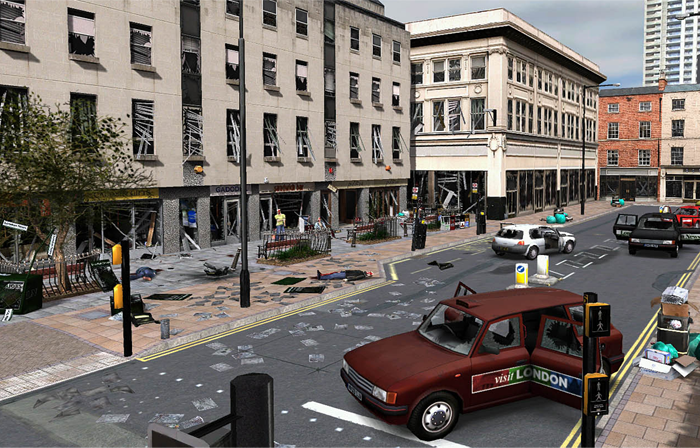
\includegraphics[scale=0.5]{tics/images/triage.png}
\caption{Ambientación de Triage}
\label{fig:triage}
\end{figure}

\emph{Triage Trainer} se desarrolla \fixme{en una escena de explosión}{Refinar,
    decir algo más intermedio, y no empezar por detalles} en una calle
(ver~\ref{fig:triage}) la cual es un incidente mayor, y está diseñado para
formar profesionales que puedan participar en una escena de un incidente de este
tipo (médicos, enfermeros, paramédicos, rescatistas). Los jugadores deben
realizar un triage, es decir, evaluar el grado de las lesiones de víctima, las
cuales son generadas aleatoriamente, utilizando los protocolos y controles
médicos adecuados, además de priorizar a las víctimas para el tratamiento. La
apariencia física de cada víctima es imitada con precisión como los signos
vitales, los síntomas y sobre todo los patrones de tiempo para el deterioro de
las lesiones, es decir, la condición de una víctima cambia de forma realista con
el tiempo (ver~\ref{fig:triage_patient1}).

\begin{figure}[ht!]
\centering 
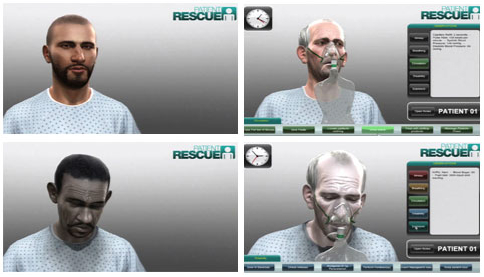
\includegraphics[scale=0.5]{tics/images/patient_side.jpg}
\caption{Evolución de un paciente en Triage}
\label{fig:triage_patient1}
\end{figure}

Al finalizar cada simulación los jugadores reciben retroalimentación acerca de
su rendimiento, incluyendo la precisión de sus chequeos, si los pacientes fueron
priorizados en el orden correcto y el tiempo que les llevó completar el triage,
en comparación con la de un experto.

La retroalimentación de los participantes que utilizaron Triage Trainer sugiere
que el mismo cumplió exitosamente sus fines. Los jugadores asociaron su
experiencia en el videojuego con su experiencia en el mundo real y muchos de ellos
sentían que realmente estaban allí. Se espera que los jugadores puedan tomar
decisiones bajo presión, lo que ayudará a su desarrollo cognitivo. También se
observó que los jugadores tienden a discutir sus experiencias con sus compañeros
de curso, lo que también podría tener un impacto en su aprendizaje.

Un elemento que no fue evaluado por \emph{TruSim} debido a que no era
logísticamente posible fue el impacto de las pruebas en la retención del
conocimiento y el cambio de comportamiento de los
jugadores\cite{education:games}. 


\subsubsection{SimVenture}

\begin{itemize}
\item \textbf{Tipo:} Juego de simulación de negocios.
\item \textbf{Destinatarios:} Personas de 14 a 30 años.
\item \textbf{Contenido:} Las realidades de la creación y funcionamiento de un
    negocio.
\item \textbf{Desarrollador:} \emph{Venture Simulations.}
\end{itemize}

En el inicio del videojuego (ver~\ref{fig:simventure_tutorial}), a los jugadores se
les brinda informaciones y antecedentes para que que se ubiquen en escena. Ellos
deben empezar a dirigir su propio negocio en su casa de fabricación y venta de
computadoras, mientras deben mantener un trabajo de tiempo completo
independiente. El videojuego lleva a los jugadores a la ejecución de un negocio en su
propia casa y a la extensión del mismo a más locales, lo que requiere
contratación de personal. Los jugadores son capaces de avanzar en el videojuego a
través del aprendizaje de los elementos importantes de la empresa, organizadas
en cuatro categorías: organización, ventas/marketing, finanzas y operaciones.
Los jugadores toman decisiones acerca de las actividades dentro de estas áreas y
observan los resultados de sus acciones. 

\begin{figure}[ht!]
\centering 
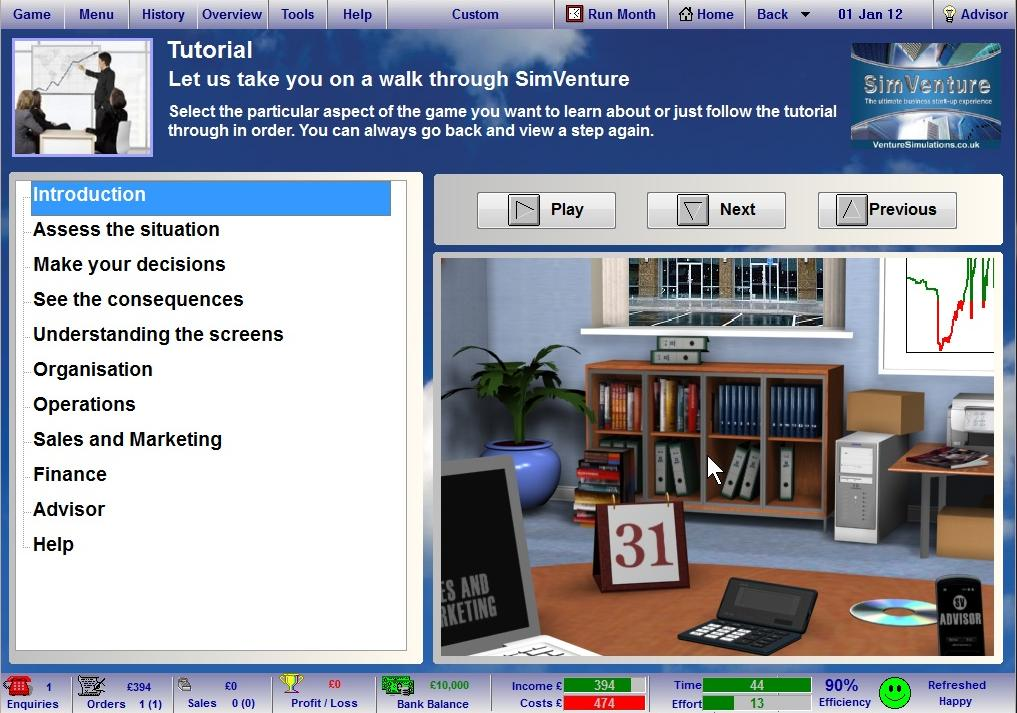
\includegraphics[scale=0.5]{tics/images/simventure-tutorial.jpg}
\caption{Tutorial de SimVenture}
\label{fig:simventure_tutorial}
\end{figure}

Los jugadores obtienen retroalimentación sobre un número de diferentes
parámetros. En un nivel básico, se puede simplemente revisar la cantidad de
ingresos que están generando. Además de esto, el éxito puede ser medido por la
cantidad de pedidos que han recibido para sus productos. También se proporciona
retroalimentación visual para representar la eficiencia de la organización y su
felicidad como individuo.

\emph{Phil Warren}, director de estudios de negocios en \emph{Snaith School}, ha
utilizado \emph{SimVenture} como complemento al plan de estudios. Según el
mismo, el plan de estudios por lo general sólo requiere que los estudiantes
aprendan sobre los diversos elementos del negocio de forma aislada, sin embargo
en la realidad, cualquier decisión que se tome en una de las partes de un
negocio tiene efecto en las demás. \emph{SimVenture} se vio como una oportunidad
de aplicar los conocimientos aprendidos en clase en una actividad práctica,
además se observó que permitir que los estudiantes jueguen en pares da un
espacio para la discusión en torno a las decisiones y aprenden de sus errores
juntos\cite{education:games}.

\section{Actualidad}

La relación de los videojuegos con el aprendizaje surge en los años $80$ y ha llegado
hasta la actualidad en plena efervescencia, siendo aplicados en casi todos los
ámbitos de la educación tanto formal como no formal. Los juegos serios para el
entrenamiento de habilidades se pueden considerar una evolución de las técnicas
de entrenamiento basadas en la realidad virtual que se desarrollaron en los años
$90$ y que en la actualidad se han transformado, por su potencial motivacional,
de simulaciones puras a juegos\cite{videojuegos:gonzaleztardon}.

Al ser un área de creciente interés, existe una gran cantidad de conferencias
cuyo objetivo es el estudio de los juegos serios en la educación, se presenta un
resumen de algunas de ellas:

\begin{itemize}
\item \textbf{Games beyond Entertainment Week}: es una serie de conferencias
    cuyo objetivo es explorar los juegos serios, sus oportunidades de mercado,
    se centra en redes, promoción, desarrollo comercial. Una de sus
    conferencias, es la \emph{Games for health}, la cual se enfoca
    específicamente en el cuidado de la salud, agrupa a profesionales de la
    salud y de los juegos serios\cite{games_beyond_entertainment}.
\item \textbf{Serious games Development and Applications}: es una conferencia
    que se desarrolla desde el $2010$, apunta a coleccionar y distribuir todo el
    conocimiento relacionado a los juegos serios, para así proveer un foro de
    discusión sobre la actualidad del desarrollo de los juegos
    serios\cite{sgda}.
\item \textbf{Gaming and Learning Conference}: es una conferencia dedicada al
    estudio y aplicación de los juegos serios, incluye una presentación donde
    los desarrolladores pueden mostrar sus productos. Se interesa además en
    potenciales inversores para el desarrollo de videojuegos, así como a
    desarrolladores, investigadores y jugadores\cite{gala}.
\item \textbf{Serious Play Conference}: es una conferencia dedicada a expertos
    con poder de decisión sobre organizaciones gubernamentales, el foco
    principal de la conferencia es explorar las oportunidades, desafíos y
    potencial de juegos serios desarrollados por los
    participantes\cite{seriousplay}.
\end{itemize}

Existen otras conferencias que no se centran exclusivamente en los juegos
serios, pero que por su naturaleza incluyen presentaciones sobre el tema, por
ejemplo, la \emph{DiGRA} (\textit{Digital Games Research Association}), se
centra en el desarrollo y la investigación de los videojuegos en general, pero
se han presentado numerosos artículos relacionados a  los juegos serios; la
\emph{Vs-Games}, que trata sobre entornos virtuales y videojuegos con  aplicaciones
más allá del entretenimiento.

Estas conferencias abarcan diferentes áreas o ámbitos de aplicación de los
juegos serios, que van desde lo militar hasta el cuidado de la salud.

\subsection{Áreas de aplicación}
\label{sec:areas_aplicacion}
\observacion{Revisar si no conviene mover esto mas adelante}

A continuación se definen las áreas de utilización  más frecuentes de juegos serios, son en 
estas áreas donde los juegos serios demuestran su fortalezas,

\begin{itemize}

\item \textbf{Militar}: Los primeros videojuegos a menudo \fixme{se basaban}{}
    en lucha o combate. Durante más de $30$ años los videojuegos han sido
    reconocidos como herramientas factibles en el entrenamiento de militares. En
    $1996$ fue lanzado un videojuego llamado \emph{Marine Doom} en donde la
    tarea de los jugadores era el aprendizaje de formas de ataque, conservación
    de municiones, comunicarse con eficacia, dar órdenes al equipo de trabajo
    entre otros. De esta manera tuvo lugar una forma de entrenamiento más
    atractivo, sin el costo, dificultad, riesgos e inconvenientes que implicaría
    el mismo entrenamiento en un entorno real. Además se podían crear
    situaciones que en el mundo real serían muy difíciles de replicar y donde
    los errores pueden ser catastróficos además, permite la repetición hasta
    alcanzar la maestría\cite{education:games}.

    \observacion{Refinar, mover más adelante}
\item \textbf{Salud}: Este tipo de videojuegos son cada vez mayores, los juegos
    de salud se utilizan para la formación de profesionales basada en la
    simulación. En $2008$ el Centro de Simulación \emph{Hollier} en
    \emph{Birmingham}, Reino Unido, realizó una prueba que permitió a médicos
    jóvenes experimentar y entrenar para diversos escenarios médicos a través de
    maniquíes virtuales como pacientes, de este modo el aprendizaje se da por la
    experiencia. En su disertación, \emph{Roger D. Smith}, realizó una comparación
    entre la enseñanza tradicional y la formación mediante realidad virtual y el
    uso de herramientas basadas en la tecnología de videojuegos en cuanto a la
    cirugía laparoscópica. Como conclusión afirmó que lo último era más barato,
    requería menos tiempo y que permitió menos errores médicos cuando los
    médicos se presentaban en una cirugía real debido a, entre otras cosas, la
    posibilidad de repetición de la experiencia sin riesgo
    alguno\cite{education:games}. 

\item \textbf{Juegos corporativos}: Este tipo de videojuegos se han utilizado
    para la selección de personal, la mejora de comunicación entre los
    directivos y su personal de confianza, y la formación de nuevos empleados.
    Un ejemplo de estos videojuegos es el \emph{INNOV8} de \emph{IBM} que ayuda
    en el entrenamiento de los estudiantes acerca de la gestión de procesos de
    negocios. Los juegos serios pueden ser utilizados incluso para elaborar
    planes de negocios\cite{education:games}. 

\end{itemize}




%\chapter{Definición del Problema}

Este capitulo define el problema en el cual se enfoca la presente tesis, el
capitulo define el estado actual de la enseñanza a futuros profesionales de
enfermería, y específicamente se centra a los profesionales formados por el
\Gls{iab}. 

Primeramente se muestra, en la sección~\ref{sec:plan_estudio}, como se
estructura la carrera de enfermería, mostrando el plan de estudios, y las
competencias que debe tener el profesional de enfermería recién egresado.

Como la enfermería es una profesión técnica, se hace una breve reseña de los
métodos de enseñanza fuera del aula que se utilizan actualmente, en el \Gls{iab}
se utilizan dos de ellos, prácticas en un laboratorio especializado
(sección~\ref{sec:practica_lab}) y prácticas de campo
(sección~\ref{sec:practica_hos})\footnote{Son prácticas que se realizan con
    pacientes reales en hospitales escuela y otros hospitales con los que el
    \Gls{iab} tiene convenios.}.

Para evaluar el rendimiento y aprendizaje de los alumnos, el \Gls{iab} utiliza
un examen teórico, además cada alumno debe completar una cantidad de horas
mínimas por materia técnica, y además debe completar ciertas actividades en
estas prácticas, esto es definido y mostrado en la
sección\ref{sec:problema_evaluacion}.

La definición del problema inicia en la sección~\ref{sec:problemas_actuales},
donde se describen los principales inconvenientes que tiene la metodología
actual, se utilizan dos puntos de vista para analizar los potenciales problemas,
la perspectiva del alumno y de las competencias básicas que debe adquirir.


La enfermería es un campo amplio, que cuenta con innumerables procedimientos que
los alumnos aprenden y perfeccionan durante su vida académica, en la
sección~\ref{sec:definicion_criterios} se definen los criterios utilizados para
seleccionar aquellas prácticas que serán simuladas como parte de la solución.

En la sección~\ref{sec:seleccion_escenas} se describen los motivos por los
cuales las escenas fueron seleccionadas, explicando sus ventajas y desventajas,
con respecto a las metodologías actuales, y finalmente, en la
sección~\ref{sec:problema_requisitos} se definen cuales son los requisitos a
tener en cuenta a la hora de desarrollar la solución\todox{Ver si no hay una
    mejor manera de definir la sección de requisitos.}.

\section{Plan de estudio}
\label{sec:plan_estudio}

La carrera de licenciatura en enfermería en el \Gls{iab} tiene una duración de 4
años, es presencial y tiene una carga total de 3745 horas. Cada alumno debe
aprobar 57 materias y las mismas son anuales.

Para completar todas las horas necesarias, las clases inician en la mañana y
culminan en la tarde. La mayoría de las materias son teóricas, recién desde
segundo curso acceden a los laboratorios especializados del instituto, y desde
el tercer año realizan prácticas de campo en hospitales escuela y hospitales con
los cuales el \Gls{iab} tiene convenios.

El perfil del egresado de la carrera de licenciatura en enfermería,
es\cite{iab:enfermeria}:

\begin{displayquote}

El profesional egresado de la Licenciatura en Enfermería será capaz de
desempeñar eficientemente el saber teórico y práctico en el campo de su
profesión, valorar las necesidades y problemas bio-psico-sociales y espirituales
del individuo, familia y comunidad, brindando apoyo y proponiendo alternativas
de solución, practicar los valores de honradez, solidaridad y respeto al ser
humano en la prestación de servicios de la salud.

\end{displayquote}

Existen tres formas principales de enseñanza dentro del \Gls{iab}, las clases
presenciales, las prácticas de laboratorio y las prácticas de campo.

Los alumnos se dividen en secciones, actualmente existen tres secciones, de $50$
alumnos cada una, la mayoría de las asignaturas cuentan con un trabajo práctico
que debe ser presentado y aprobado para obtener una habilitación para rendir el
examen final.

El plan de estudios se centra en las \emph{competencias básicas} que debe tener
cada alumno al finalizar la materia, estas competencias son facilitadas al
inicio de cada asignatura a los alumnos, y todo el desarrollo de la materia se
centra en su obtención.

Las competencias básicas son los conocimientos teóricos y prácticos que debe
tener todo profesional de enfermería recién egresado, estas competencias son el
eje central de la carrera y en la obtención de las mismas se centran todas las
actividades curriculares y no curriculares (congresos, encuentros, etc)
realizadas por el \Gls{iab}.

\section{Prácticas en laboratorios}
\section{Prácticas de enfermería}
\label{sec:practica_hos}

Se definen las prácticas profesionales como\cite{iab:est_enfemeria}:

\begin{displayquote}

Son prácticas de enfermería aquellas actividades de integración y de aplicación
de los conocimientos teóricos adquiridos y las destrezas y habilidades,
acercando al estudiante a una realidad concreta que le permita una experiencia
vivencial. Ellas pueden ser desarrolladas en arte de enfermería, así como en los
servicios de salud de diferentes niveles de complejidad, instituciones públicas
y privadas, establecimientos, hogares y comunidad.

\end{displayquote}

Las prácticas de campo son aquellas prácticas profesionales que son realizadas
por los alumnos con pacientes humanos y en hospitales, bajo supervisión de un
profesional y bajo una continua evaluación de sus acciones, las mismas son
llevadas a cabo una vez que los alumnos finalizan las prácticas de laboratorio.

Los alumnos del \Gls{iab} participan en prácticas de campo en diferentes
hospitales dependiendo de las necesidades de cada materia, por ejemplo, los
alumnos de \textit{Enfermería en Urgencias} realizan sus prácticas en el
\textit{Centro de Emergencias Médicas}, otros hospitales utilizados, son el
\textit{Hospital de Clínicas}, y diversos hospitales del \textit{Instituto de
    Previsión Social}.

Para controlar y medir la evolución de los estudiantes existe un grupo de
profesores cuya función es guiar a los alumnos durante las prácticas de campo,
este grupo de profesores son denominados \textbf{instructores}.

Las prácticas se realizan en grupos que varían de 4 a 10 alumnos, dependiendo de
la disponibilidad de instructores y de si el área es crítica o no\footnote{Se
    dice que un paciente esta en estado crítico si su vida depende de un
    procedimiento externo, como una transfusión de sangre, un área se considera
    crítica si los pacientes en su mayoría son críticos}, un instructor puede
manejar más de un grupo en diferentes horarios. 

Cada instructor posee un planilla por alumno donde se realiza el seguimiento de
sus actividades. La creación de esta planilla de actividades es responsabilidad
del instructor, el instructor debe basarse en las competencias básicas de la
asignatura y la misma es validada por la dirección de la carrera, y se considera
que un alumno ha adquirido la pericia necesaria para una asignatura solo sí pudo
completar la planilla del instructor de dicha asignatura. Son registradas todas
las actividades del alumno, pero solo cuentan para el progreso final aquellas
que son realizadas con la pericia necesaria.

La cantidad de alumnos, hace que la práctica de una asignatura rara vez se
realice en un solo hospital, para asignaturas críticas, debe haber
aproximadamente 35 grupos de estudiantes.

%! TEX root = ../main.tex
\section{Evaluación de lo aprendido}
\label{sec:problema_evaluacion}
\observacio{Reformular el título, no se entiende (por el estudiante? O
    ustedes?)}


\observacion{Resumir más los siguientes 4 párrafos} 

Como dicta su perfil, un egresado debe ser capaz de desempeñar eficientemente su
profesión, el mecanismo que se utiliza para garantizar esto, son las
evaluaciones.

Una evaluación es un proceso que permite verificar el grado del progreso del
estudiante en el logro de los objetivos propuestos en cada
asignatura\cite{iab:est_enfemeria}, existen tres tipos de evaluaciones, exámenes
parciales, exámenes finales y evaluación de la práctica de campo.

La cantidad de evaluaciones parciales esta determinada por la materia y el
consenso de los profesores titulares\cite{iab:est_enfemeria}, la cantidad de
exámenes parciales varía desde dos hasta cuatro por asignatura\footnote{Se
    define examen parcial aquel que mide el rendimiento del periodo
    correspondiente\cite{iab:est_enfemeria}.}.

En cuanto a las evaluaciones finales, existen tres periodos en los cuales un
alumno puede rendir el examen final.

Cada alumno necesita de un $75\%$ de asistencia presencial para tener derecho a
las evaluaciones, así mismo, cada alumno requiere como mínimo $80\%$ de la carga
horaria en prácticas profesionales, el $20\%$ restante lo debe cumplir en un
periodo establecido por el \Gls{iab}.

\fixme{En cuanto a la evaluación de la práctica de campo, el enfoque es
    subjetivo, es decir depende exclusivamente del instructor de la práctica
    determinar si un alumno cuenta o no con la pericia necesaria.}{Concentrarse
    en esto}

La calificación final de materias no profesionales, se obtiene de la siguiente
manera\cite{iab:est_enfemeria}:

\begin{itemize}
    \item $30\%$ de la sumatoria de las pruebas parciales.
    \item $20\%$ de los trabajos prácticos.
    \item $50\%$ del examen final, siempre y cuando el alumno haya obtenido
        una calificación mínima de $2$.
\end{itemize}

\observacion{Que tan importantes son las prácticas? En la evaluación y en la
    vida real. Cocho: poner acá lo que dijo Miguela que la gente tiene miedo}

Para materias profesionales, se utiliza la misma escala descrita anteriormente,
y además se promedia el resultado con la calificación de la práctica
profesional\cite{iab:est_enfemeria}, teniendo en cuenta que un alumno con
calificación $1$ en el examen final tiene automáticamente la nota $1$ en la
materia\cite{iab:est_enfemeria}.

La escala es del $60\%$ para asignaturas no profesionales y del $75\%$ para
materias profesionales, la escala que se utiliza es del $1$ al $5$.

El objetivo final de estas evaluaciones es el de evaluar si un alumno comprende
y tiene la pericia necesaria en todas las competencias básicas de dicha
asignatura.

\section{Problemas actuales}

\section{Definición de criterios}
\label{sec:definicion_criterios}

Teniendo en cuenta lo expuesto en las secciones anteriores, se realizaron varias reuniones con la coordinadora de la carrera de Enfermería del \Gls{iab}, Lic. Miguela Hermosilla y otros profesores encargados de las
prácticas de laboratorio y campo de las diversas materias de la carrera.

En estas reuniones se valoraron varios procedimientos que podían ser simulados o presentados en la
propuesta de solución que será descripta en la sección siguiente. De todos los procedimientos evaluados
y discutidos se eligieron dos ya que resulta imposible simular todos los procedimientos de enfermería
existentes. Los principales criterios para la selección fueron los siguientes:

\begin{itemize}
\item Las situaciones simuladas no deben ser muy afectadas por las limitaciones que conllevan las 
características que presentara la solución propuesta.
\item Las situaciones simuladas deben ser de utilidad para los usuarios de la población objetivo.
\item Las situaciones simuladas no deben ser muy complejas ni largas.
\item Las situaciones simuladas deben tener pasos bien definidos.
\item Las situaciones simuladas deben ser difíciles de representar con realismo en un aula o laboratorio.
\end{itemize}



\section{Selección de escenas}
\section{Requisitos de la solución}
\label{sec:problema_requisitos}

La solución propuesta debe cumplir con las condiciones que se citan a continuación:

\subsection{Generales}
\begin{itemize}
\item Se debe utilizar la plataforma Unity3D como herramienta para la creación del entorno.
\item Se debe permitir al jugador poder utilizar el entorno virtual en el momento y lugar que desee es decir, 
se le debe proveer ubicuidad.
\item Las escenas presentadas, junto con lo elementos dentro de ellas deben ser representados en tres dimensiones y
lo mas realista posible.
\item Cada escena representara un procedimiento de enfermería que debe ser realizado por el jugador.
\item El entorno debe permitir al jugador decidir libremente las acciones que quiere realizar.
\item El entorno no debe brindar pistas al jugador acerca de la forma en la que se deben realizar las procedimientos.
\item El entorno debe brindar al jugador información final acerca de su desempeño en la escena.
\item La selección de una escena debe ser realizada mediante un menú ubicado en la pantalla principal o de bienvenida.
\item Se debe permitir que el movimiento de la cámara sea manipulado por el jugador para rotación y aumento de tamaño de la escena.
\item El final de una partida debe indicarse mediante un botón en un menu ubicado en la pantalla principal de la escena.
\end{itemize}

\subsection{Interacción del jugador con los objetos}
\begin{itemize}
\item La selección de objetos se debe realizar mediante un menú ubicado en la pantalla principal de la escena.
\item El objeto actualmente seleccionado se representara mediante un imagen en la escena.
\item Los objetos utilizados como instrumentos necesarios para la realización de un procedimiento deben
utilizarse solo uno a la vez.
\item Un objeto seleccionado debe poder des-seleccionarse volviendo a presionar el botón que le representa en el 
menú.
\end{itemize}

\subsection{Interacción entre objetos}
\begin{itemize}
\item Para realizar acciones sobre el paciente haciendo uso del objeto seleccionado, se debe manipular el objeto
directamente.
\item Para ubicar el objeto seleccionado en la escena se debe tocar sobre el paciente en el lugar donde se desea
que aparezca.
\item Los objetos tendrán menú contextuales para aquellas acciones mas complejas de realizar.
\end{itemize}

\subsection{Acciones del jugador}
\begin{itemize}
\item Las acciones realizadas por los jugadores en el entorno virtual deben ser registradas.
\item Cada acción realizada por el usuario debe ser validada por el entorno, de forma a ofrecer información
correcta acerca de sus logros al final de la partida.
\item La validez de una acción puede requerir en algunos casos que se hayan hecho algunas acciones previas e incluso con cierto orden.
\item No se deben dar pistas o mensajes al jugador durante la partida cuando este realice incorrectamente una acción.
\item Se debe contar con botones para las acciones que modifican el estado del jugador.
\end{itemize}


%\chapter{Alcance y requerimientos}
\label{chap:requerimientos}

Realizada la propuesta de solución de este trabajo de grado, a continuación se presenta 
el alcance de la solución y los requerimientos que debe cumplir para alcanzar su
objetivo pedagógico.
%Realizada la propuesta de solución en la que se centra este trabajo de grado,
%se describen los requerimientos necesarios para que la misma cumpla su objetivo
%pedagógico.

Primeramente se definen los criterios de selección de los procedimientos a simular, 
como el área de enfermería es muy amplia, se eligen procedimientos que se ajustan a 
estos criterios y a los objetivos del presente trabajo. Una vez seleccionados los 
procedimientos, se describen sus detalles y las competencias básicas que están definidas 
en el plan de estudio relacionadas a cada procedimiento. 

A fin de determinar el alcance de la solución, se describen hipótesis y factores
que limitan lo que es necesario incluir y el nivel de detalle de la simulación.

El último aspecto tratado en este capítulo es el de los requisitos transversales
que debe cumplir la solución, como requisitos de jugabilidad, lo que incluye manipulación de
la cámara, interfaz, etc; así como también requisitos pedagógicos, como la
retroalimentación y muestra de información.

%! TEX root = ../main.tex
\section{Definición de criterios}
\label{sec:criterios}

Se realizaron varias reuniones con la coordinadora de la carrera de Licenciatura
en Enfermería del \Gls{iab} y profesores encargados de las prácticas de
laboratorio y campo de diversas materias de la carrera. De estas reuniones, y
del plan de estudios de la carrera de enfermería, se extraen procedimientos que
pueden ser simulados, cuya aceptación y validación son realizados por  
profesores del área de enfermería del \Gls{iab}.

De los procedimientos evaluados y discutidos se eligen dos ya que la variedad y
cantidad de procedimientos de enfermería existentes es muy alta e incluirlos
todos a la solución está fuera del alcance de este trabajo. Los principales
criterios para la selección de los procedimientos son los siguientes:

\begin{itemize}

    \item \textbf{Deben adecuarse a las limitaciones de la tecnología} 

    Escenarios que requieren la simulación de órganos internos, psicología
    humana, etc, pueden requerir una complejidad adicional a la hora de
    implementar la simulación, complejidad que escapa al alcance del presente
    trabajo.

    \item \textbf{Deben de ser de utilidad para los alumnos} 
    
    Deben ser procedimientos comunes en la vida profesional de un enfermero, o
    que no sea posible realizar practicas frecuentes. 

    Al ser una profesión relacionada con la salud, existen múltiples factores
    que dificultan las prácticas de enfermería, como la salud del paciente, la
    salud del profesional, enfermedades o procedimientos poco frecuentes, etc.

\item \textbf{Los procedimientos seleccionados no deben ser complejos ni
        extensos}. 

    Las simulaciones cortas permiten poder ser utilizadas en cualquier momento,
    sin ser interrumpidas. En cuanto al nivel de detalle del entorno, los
    entornos complejos dificultan la atención del
    usuario\cite{videojuegos:gonzaleztardon}, por ello, los factores que son
    simulados deben ser los suficientes para permitir al usuario sentirse dentro
    de la misma, pero no deberían ser muy complejos, sino, el usuario desviaría su
    atención hacia los detalles.

\item \textbf{Deben tener pasos definidos}
    
    Si el procedimiento tiene un objetivo claro, y un conjunto de pasos
    previamente definidos y previsibles, se facilita la aceptación del mismo por
    los profesores, es decir, es más fácil realizar una validación de la
    simulación.

    Hay un compromiso entre la validación de la simulación y la libertad de
    exploración de los usuarios, el escenario elegido debe tener pasos
    definidos, pero a la vez debe permitir al alumno explorar el escenario y
    tomar caminos alternativos.

\item \textbf{Deben ser difíciles de representar con realismo en un aula o
        laboratorio}

    Los laboratorios del \Gls{iab} cuentan con diferentes herramientas que
    facilitan ciertos procedimientos, pero estos no pueden abarcar el amplio
    rango que cubren los procedimientos de enfermería, por ello se debería
    elegir un procedimiento que muestre las ventajas de la tecnología y técnicas
    propuestas, el procedimiento tiene que representar un desafío a las técnicas
    actuales, este desafío puede ser 
    \begin{enumerate*}[label=\itshape\alph*\upshape.]
    \item técnico, como falta de herramientas, como equipos médicos, maniquíes,
        etc, o,
    \item humano, como falta de pacientes con la patología deseada.
    \end{enumerate*}
    
\end{itemize}

%! TEX root = ../main.tex
\section{Selección de procedimientos}
\label{sec:seleccion_escenas}

Con los criterios definidos \fixme{se seleccionaron}{tiempo} dos procedimientos de enfermería,
los cuales serán incluidos en la solución. A continuación se fundamentan
\fixme{tales}{?} elecciones y se entra en detalle acerca de los procedimientos
seleccionados.

%Estos procedimientos son incluidos en la solución creando escenarios dentro del
%videojuego que permitan realizarlos, es así que cada procedimiento es
%representado con escenarios y escenas diferentes.

\subsection{Extracción de muestras de sangre}
\label{sec:hemocultivo}

El procedimiento denominado \emph{Punción venosa} es utilizado frecuentemente
para extraer muestras de sangre, es un procedimiento invasivo que ofrece un
medio directo de acceso al sistema vascular. 

La frecuencia con la que se lo utiliza esta relacionado a su utilidad para
análisis de rutina, los enfermeros lo realizan a diario y es similar a otros
procedimientos como la puesta de una vía intravenosa.

El procedimiento se puede resumir en el proceso de punzar con una jeringa el
brazo al paciente, extraer sangre y retirarla. Si bien estos pasos pueden
parecer sencillos, existen una gran cantidad de factores que definen si el
procedimiento fue realizado correctamente, entre ellas podemos encontrar a
factores de bioseguridad\footnote{La bioseguridad es la aplicación de
    conocimientos, técnicas y equipamientos para prevenir a personas,
    laboratorios, áreas hospitalarias y medio ambiente de la exposición a
    agentes potencialmente infecciosos o considerados de riesgo biológico.},
como la esterilización correcta de los materiales; sociales, como la explicación
correcta del procedimiento al paciente, etc.

Este procedimiento es considerado como uno de los apropiados de acuerdo a la
apreciación de los profesionales del \Gls{iab}, además: 

\begin{itemize}
\item El mismo posee pasos bien definidos que deben ser seguidos por el
    profesional de enfermería.
\item La complejidad del procedimiento no es muy alta, sus pasos son
    susceptibles de equivocaciones, especialmente en lo que se refiere a la
    bioseguridad. 
\end{itemize}



\subsubsection{Evaluación al alumno}

% Ver si esta bien explicar esta sección, o ir nomas al grano
\fixme{En este punto se explican las}{mejorar} competencias básicas de este
procedimiento con respecto al plan de estudio de los estudiantes de enfermería
del \Gls{iab} y los criterios relacionados al procedimiento según la planilla de
práctica que poseen los profesores instructores para evaluar al alumno.

La competencia básica que engloba al procedimiento de extracción de sangres es:

\begin{itemize}
\item Ayudar en procedimientos invasivos
\end{itemize}

Los elementos que son almacenados en la planilla de los instructores, son:
%\pregunta{Esto fue extraído de planilla del instructor, se puede poner una
%referencia la anexo}
% RESPUESTA SÍ

\begin{itemize}
\item Informe al paciente acerca del procedimiento que va a ser
    realizado.
\item Preparación de material para la técnica aséptica.
\item Lavado de manos.
\item Calzado de guantes, chaleco estéril, tapaboca y gorro.
\item Preparación de campo.
\item Punción del brazo, extracción de sangre, compresión de zona de punción.
\item Cambio de aguja.
\item Introducción de la muestra en un frasco preparado para tal efecto.
\item Retiro de materiales y equipo de protección personal.
\item Etiquetado y envío a laboratorio.
\end{itemize}

Es decir, estos son los criterios que debe cumplir cualquier estudiante
para poder aprobar la práctica.

\subsubsection{Protocolo del procedimiento}
\label{sec:hemocultivo_protocolo}

\observacion{Muy seco}


\observacion{Sujeto, verbo y predicado, La siguiente sección comprende todos los
    pasos}

La descripción formal del procedimiento, con todos los pasos necesarios
para poder llevar a cabo los criterios requeridos según~\cite{oms:extraccion}
y los profesores del \Gls{iab}, se observan en la~\ref{fig:proc_hemocultivo}, y
son los siguientes:

\begin{figure}
\centering
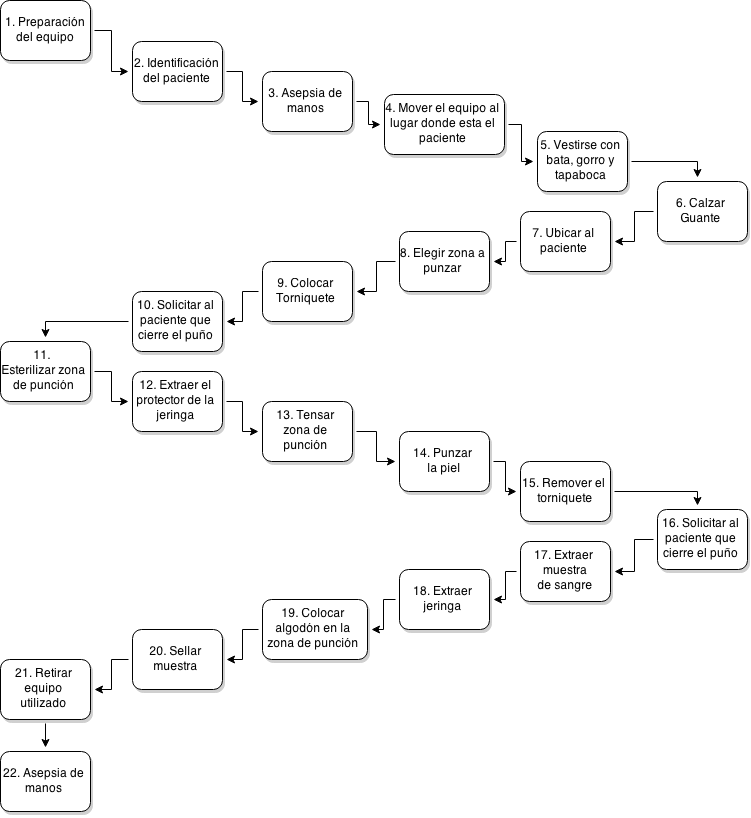
\includegraphics[scale=0.5]{requerimientos/images/hemocultivo.png}
\caption{Procedimiento de extracción de sangre.}
\label{fig:proc_hemocultivo}
\observacion{Se explica en algún lugar que no es necesariamente lineal? Por que
    se simplifica acá?}
\end{figure}

\begin{enumerate}
\item Preparar el equipo, lo que incluye seleccionar la jeringa adecuada.
\item Identificar al paciente, presentarse y explicarle el procedimiento que va
    a ser realizado.
\item Asepsia de las manos.
\item Llevar el equipo a la unidad en donde se encuentra el paciente.
\item Vestirse con bata estéril, tapaboca y gorro.
\item Calzarse los guantes.
\item Ubicar al paciente en posición adecuada, esto es, el brazo debe estar
    extendido y lo mas relajado posible.
\item Elegir la zona a puncionar, para ello se debe palpar la vena para
    averiguar sus características.
\item Colocar el torniquete, 6 a 10 centímetros por encima de la zona de
    punción.
\item Solicitar al paciente que cierre el puño.
\item Esterilizar la zona de punción.
\item Extraer el protector de la aguja.
\item Tensar la zona de punción.
\item Puncionar la piel con la aguja hacia arriba. La aguja se introduce con un
    ángulo de $10$ a $20$ grados.
\item Remover el torniquete.
\item Solicitar la apertura del puño.
\item Extraer la muestra de sangre necesaria.
\item Presionar y extraer la aguja.
\item Colocar algodón con alcohol en el punto de punción.
\item Sellar la muestra y enviarlo a su destinatario.
\item Retirar el equipo utilizado, incluyendo bata, tapaboca, gorro y guantes.
\item Asepsia de las manos.
\end{enumerate}

\subsection{Valoración de la escala de Glasgow}
\label{sec:glasgow}

La escala de Glasgow es utilizada como una herramienta de valoración objetiva
del estado de conciencia de pacientes en estado crítico\cite{protocolo}. La
escala consiste en la evaluación de tres criterios de observación clínica,
los cuales son: 
\begin{enumerate*}[label=\itshape\alph*\upshape.]
\item la respuesta ocular
\item la respuesta verbal, y
\item la respuesta motora.
\end{enumerate*}

\begin{table}[!hbt]
\centering
\begin{tabular}{llr}
\toprule
\textbf{Severidad} & 
\textbf{Puntuación} \\ 
\midrule
 Leve & 13 a 15 \\
 Moderado & 9 a 12 \\
 Grave & 3 a 8 \\
\bottomrule
\end{tabular}
\caption{Escala de valoración del estado del paciente\cite{helmick2007mild}.}
\label{tab:seleccion_glasgow_estado}
\end{table}

El puntaje que determina el estado del paciente se obtiene sumando la valoración
de cada una de las respuestas, en la figura~\ref{tab:seleccion_glasgow_estado}
se observan los posibles diagnósticos. A la vez cada respuesta se evalúa
mediante una escala independiente una de otra, donde cada respuesta se puntúa
con un número\cite{glasgow:doc}, los valores de cada respuesta se observan en las
tablas~\ref{tab:seleccion_glasgow_respuestas_ocular},~\ref{tab:seleccion_glasgow_respuestas_motor}
y~\ref{tab:seleccion_glasgow_respuestas_verbal}.

\begin{table}[!hbt]
\centering
\begin{tabular}{lr}
\toprule
\textbf{Apertura ocular} & \textbf{Valor} \\
\midrule
Espontánea & 4 \\
Al hablar & 3 \\
Al dolor & 2 \\
Ausente & 1 \\
\bottomrule
\end{tabular}
\caption{Valoración de las distintas respuestas en la escala de Glasgow,
    respecto a la reacción ocular}
\label{tab:seleccion_glasgow_respuestas_ocular}
\end{table}

\begin{table}[!hbt]
\centering
\begin{tabular}{lr}
\toprule
\textbf{Respuesta motora} & \textbf{Valor} \\
\midrule
Obedece & 6 \\
Localiza & 5 \\
Retira & 4 \\
Flexión anormal & 3 \\
Extiende & 2 \\
Ausente & 1 \\
\bottomrule
\end{tabular}
\caption{Valoración de las distintas respuestas en la escala de Glasgow,
    referentes a las respuestas motoras}
\label{tab:seleccion_glasgow_respuestas_motor}
\end{table}

\begin{table}[!hbt]
\centering
\begin{tabular}{lr}
\toprule
\textbf{Respuesta verbal} & \textbf{Valor} \\
\midrule
Orientada & 5 \\
Confusa & 4 \\
Palabras inapropiadas & 3 \\
Palabras incomprensibles & 2 \\
Ausente & 1 \\
\bottomrule
\end{tabular}
\caption{Valoración de las distintas respuestas en la escala de Glasgow
    referentes a la respuesta verbal}
\label{tab:seleccion_glasgow_respuestas_verbal}
\end{table}

El procedimiento se utiliza cuando existe un paciente con un estado de
conciencia indefinido, normalmente después de un accidente donde el paciente
recibió un traumatismo severo. El profesional que se encarga de evaluar debe
verificar el estado del paciente mediante
\begin{enumerate*}[label=\itshape\alph*\upshape.]
\item preguntas sencillas,
\item estímulos, e
\item inspecciones de partes del cuerpo.
\end{enumerate*}. 
Una vez que se obtiene una valoración individual para los aspectos
motor, ocular y visual del paciente, se obtiene la suma de las valoraciones y se
obtiene un puntaje para el estado del paciente.

El procedimiento de diagnóstico utilizando la escala de Glasgow es considerado
como uno de los apropiados para la solución propuesta ya que:

% Recheckear esto
\begin{itemize}
\item Permite la exploración del entorno pues hay diferentes formas de evaluar cada
    estado del paciente.
\item Es rara vez utilizado, pues las condiciones necesarias para que un paciente 
    requiera que se le realice este procedimiento son críticas, son
    escasas las oportunidades presentadas a los estudiantes durante sus
    prácticas de campo. 
\item La cantidad de reacciones que evalúa el procedimiento es muy alta,
    así, es difícil que un alumno pueda evaluar todos los posibles estados en
    sus prácticas de campo.
\item No es un procedimiento complejo, pues no requiere la manipulación de
    elementos, aún así requiere pericia y debe ser realizado en el menor tiempo
    posible.
\end{itemize}


\subsubsection{Evaluación al alumno}

\fixme{Se describen}{Mejorar} las competencias básicas de \enquote{Evaluación
    del alumno utilizando la escala de Glasgow} según el plan de estudios de los
estudiantes de enfermería del \Gls{iab}, la planilla de práctica que poseen los
instructores, el protocolo para llevar a cabo el procedimiento
según~\cite{protocolo} y los profesores del \Gls{iab}.

La competencia básica que incluye a la evaluación del paciente mediante la
escala de Glasgow es:

\begin{itemize}
\item Identificar actividades de cuidados según problemas urgentes principales.
\end{itemize}

En el gráfico~\ref{fig:proc_glasgow} se observan los pasos necesarios para
realizar la evaluación utilizando la escala de Glasgow\cite{protocolo}. Dentro del
procedimiento definido en la práctica profesional los criterios son:

\begin{figure}
\centering
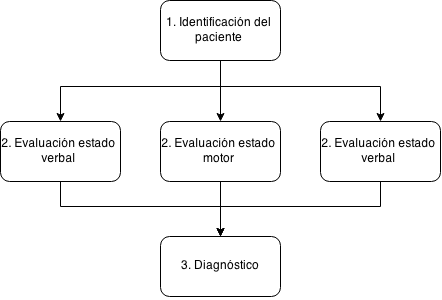
\includegraphics[scale=0.5]{requerimientos/images/glasgow.png}
\caption{Evaluación de Glasgow.}
\label{fig:proc_glasgow}
\end{figure}

\begin{itemize}
\item Control de signos vitales.
\item Inspección cefalocaudal, 
\item Evaluación utilizando escala de Glasgow.
\item Preparación del equipo según prioridad del problema
\item Analizar su participación en las actividades.
\item Fundamenta científicamente sus decisiones.
\end{itemize}

Se observa que el punto \enquote{Evaluación utilizando escala de Glasgow}, es un
paso necesario para la evaluación inicial de un paciente en estado crítico.

\subsubsection{Protocolo del procedimiento}
\label{sec:glasgow_protocolo}
\observacion{Ver tesis de parra para ver como se referencia?}

El protocolo del procedimiento, según~\cite{protocolo} y los profesores del \Gls{iab}
es:

\begin{enumerate}
\item Preparación del material
\item Preparación del paciente: comprobar su identidad, mantener una ambiente
    tranquilo evitando interrupciones, requerir la atención del paciente.
\item Colocar al paciente en posición cómoda.
\item Medir la apertura ocular.
\item Evaluar la respuesta motora.
\item Medir la respuesta verbal.
\item Registrar la puntuación final obtenida.
\end{enumerate}

\section{Alcance de la simulación}
\label{sec:alcance}

Para representar los procedimientos seleccionados y descritos en la
sección\ref{sec:seleccion_escenas}, estos deben ser presentados dentro de
escenarios distintos con los elementos necesarios para poder llevarlos a cabo.
Sin embargo, por limitaciones técnicas, tecnológicas y de tiempo, no es posible
realizar una simulación de todos los pasos requeridos.

\observacion{Más énfasis en el hecho que distrae a la parte pedagógica}
Según~\cite{videojuegos:gonzaleztardon}, existe un compromiso visible entre
realismo y credibilidad, tomando en cuenta que uno de los objetivos de la
solución es la presentación de situaciones simplificadas que permitan transmitir
conocimiento, mientras más realismo exista, más detalles existirán y por
consiguiente, los usuarios tendrán que concentrarse en un mayor número de
detalles, lo que resulta contraproducente con el objetivo de la
solución\cite{videojuegos:gonzaleztardon}. Los criterios e hipótesis que se 
describirán a continuación sirven para acotar el
alcance de la simulación, definen qué se simulará y cual es del detalle
necesario para alcanzar las competencias básicas.

\fixme{A continuación se fundamentan por qué ciertos pasos serán simulados,
    representados o no simulados dentro de la solución basados en limitaciones e
    hipótesis asumidas.}{Mover esto abajo de factores limitantes}

Cada uno de los pasos están agrupados de acuerdo a cada uno de estos aspectos.

\subsection{Factores limitantes}

Se refieren a cada uno de los aspectos que determinan si un paso 
será simulado dentro de la solución. Se clasifican en tres: limitaciones técnicas, 
importancia y facilidad de realización. Estos tres aspectos que influyen en qué partes 
se simularán y qué partes se omitirán, se detallan a continuación.

\observacion{No empezar con un ejemplo.}
\begin{itemize}
\item  \textbf{Limitaciones técnicas}: 
    
    Acciones como la simulación del agua (necesarios para el lavado de manos),
    requieren de requisitos de hardware avanzados y un tiempo considerable de
    desarrollo. Las acciones que escapan al alcance del hardware, del software o
    de tiempo de los desarrolladores no son simuladas. 
    \observacio{Reformular capítulo anterior}
        
    Los pasos del procedimiento de extracción de sangre que no se simularán por 
    limitaciones técnicas son:
    \begin{itemize}
        \item Tensar la zona de punción.
        \item Ángulo de punción.
        \item Presionar el brazo en el momento en el que se introduce la jeringa.
    \end{itemize}
    
    
\item  \fixme{Importancia}{de qué?} 

    No todos los pasos definidos en el procedimiento        
    oficial son \fixme{necesarios}{mandatorios} de simular, por ejemplo, la
    colocación de los elementos cerca del lugar de trabajo, es un paso necesario
    en el procedimiento, pero es considerado un paso poco importante y fácil de
    realizar.

    La importancia es evaluada por profesionales del \Gls{iab}, los
    cuales dieron su apreciación acerca de cada aspecto simulado, el mismo
    es tenido en cuenta para determinar la importancia de cada
    acción.
    
    Los pasos del procedimiento de extracción de sangre que no se simularán por 
    no ser importantes para la simulación son:
    \begin{itemize}
        \item Llevar el equipo en la unidad donde se encuentra el paciente.
        \item Extraer el protector de la aguja.
        \item Sellar la muestra y enviarlo a su destinatario.
    \end{itemize}
    
    
\item \textbf{Facilidad de realización en la vida real o en el laboratorio}:
    \observacion{Reformular título}

    Ciertos pasos son fáciles de realizar en la vida real pero requieren un
    esfuerzo significativo para ser simulados con realismo, como preparar el
    equipo necesario.

    La facilidad que tienen los alumnos con las acciones fue determinada por
    profesores del \Gls{iab}, determinaron qué acciones son fáciles de
    realizar para los alumnos y cuáles presentan mayores dificultades en su
    vida profesional.

    Otro aspecto que influye en la facilidad de realización de los
    procedimientos es la familiarización, si los alumnos están
    familiarizados con los procedimientos, estos no son simulados.
        
    Los pasos del procedimiento de extracción de sangre que no se simularán por 
    ser fáciles de realizar por los alumnos son:
        
    \begin{itemize}
        \item Preparar el equipo.
        \item Ubicar al paciente en posición adecuada.
    \end{itemize}
    
    Los pasos del procedimiento de valoración de la escala de Glasgow 
    que no se simularán por la misma razón son:
    \begin{itemize}
    \item Preparar el material.
    \item Preparar al paciente.
    \item Colocar al paciente en posición cómoda.
    \end{itemize}
        
\end{itemize}

\subsection{Hipótesis}
\label{sec:hipotesis}
\observacion{No utilizar: existen, que debería, no son}

\fixme{Además de los pasos mencionados anteriormente, existen otros pasos que
    son necesarios representar pero no necesariamente simular de forma
    detallada,}{Mejorar} para estos pasos se formularon hipótesis basadas en
apreciaciones de los profesores del \Gls{iab} y en pruebas de usabilidad de
interfaz las cuales son detalladas en el capítulo\ref{chap:evaluacion} y cuyos
resultados se muestran en el capítulo\ref{chap:analisis}. A continuación se
detallan cada una de estas hipótesis.

% Hipótesis
\begin{itemize}
\item 
    \textbf{Comandos de voz con interfaz}:  para enviar una petición o informarle 
    sobre algo al paciente (por ejemplo, darle detalles del procedimiento), 
    no es necesario identificar las palabras del usuario, sino más bien detectar
    que ha hablado y listar las posibles acciones que se pueden realizar.
    
    Los pasos del procedimiento de extracción de sangre que son representados por 
    comando de voz son:
    
    \begin{itemize}
        \item Explicar procedimiento.
        \item Solicitar al paciente que cierre el puño.
        \item Solicitar al paciente que abra el puño.
    \end{itemize}
    
    y, los pasos del procedimiento de valoración de la escala de Glasgow 
    que son representados por la misma razón son:
    \begin{itemize}
        \item Explicar el procedimiento.
        \item Medir la respuesta ocular por medio de peticiones al paciente.
        \item Medir la respuesta verbal por medio de preguntas al paciente.
        \item Medir la respuesta motora por medio de peticiones al paciente.
    \end{itemize}

\item
    \textbf{Extracción uniforme de elementos}: para realizar la acción de extraer 
    un elemento utilizado en el paciente, se considera que realizarlo de una sola 
    manera para todos los elementos convierte a la interfaz más intuitiva.

    %\textbf{Utilización de menú contextual}: para realizar una acción con los
    %    elementos, es suficiente con presionar el mismo y seleccionar una acción
    %    de una lista de opciones, no hace falta emular todas las posibles.
    
    Los pasos del procedimiento de extracción de sangre que cumplen con la extracción 
    uniforme son:
    
    \begin{itemize}
        \item Extraer torniquete.
        \item Extraer jeringa.
    \end{itemize}
    
\item 
    \textbf{Acciones por menú}: \fixme{}{Menú? UI?} acciones como el de generar
    un estímulo doloroso al paciente tienen limitaciones técnicas para su
    simulación pero no pueden ser omitidas debido a su gran importancia en el
    procedimiento. Por lo tanto, acciones como estas son realizadas a través de
    menús contextuales.
    
    \observacion{No se debería hablar de soluciones aún}
    Los pasos del procedimiento de valoración de la escala de Glasgow que son
    importantes de simular pero poseen limitaciones técnicas son:
    \begin{itemize} 
    \item Realizar estímulos dolorosos en diferentes partes del cuerpo. 
    \end{itemize}
    
    

\item 
    \textbf{Acciones de bioseguridad}: la bioseguridad, que es un aspecto
    fundamental y transversal a todo procedimiento de enfermería. Es un área muy
    amplia y transversal a todos los procedimientos de enfermería por lo que se
    considera que simular cada acción es complejo y que sólo basta con que el
    estudiante sepa el momento en el que debe realizarse cada una de estas
    acciones y por lo mismo, es suficiente representarlas a través de opciones
    en la interfaz gráfica.
    
    Los pasos del procedimiento de extracción de sangre que son representados
    por opciones son:
    \begin{itemize}
        \item Asepsia de las manos.
        \item Vestirse con bata estéril, tapaboca estéril y gorro estéril.
        \item Calzar guantes.
        \item Extraer guantes, bata, tapaboca y gorro.
    \end{itemize}
    

\end{itemize}
% Simulados

\subsection{Pasos de exploración}

Los demás pasos no mencionados previamente deben ser simulados de forma 
integra ya que no se ven afectados por ninguna de las hipótesis y criterios previamente
descriptos.

La evaluación de estos pasos depende de elecciones que haga el usuario, por ejemplo
la elección de una zona de punción depende del usuario, existen varios lugares posibles, 
de los cuales solo algunos son válidos. 

Los pasos del procedimiento de extracción de sangre que cumplen con esto son:
\begin{itemize}
    \item Elegir zona a punzar.
    \item Colocar torniquete.
    \item Esterilizar zona de punción.
    \item Elegir la zona a puncionar.
    \item Punzar la zona con la aguja.
    \item Extraer muestra de sangre.
    \item Colocar algodón en zona de punción.
    \item Presionar zona punción con el algodón.
\end{itemize}

Los pasos de valoración de la escala de Glasgow que también cumplen con esto son:
\begin{itemize}
    \item Registrar la puntuación de la respuesta ocular.
    \item Registrar la puntuación de la respuesta motora.
    \item Registrar la puntuación de la  respuesta verbal.
    \item Registrar el diagnóstico final.
\end{itemize}



%! TEX root = ../main.tex
\section{Requisitos de la solución}
\label{sec:requisitos}

A fin de que la solución propuesta pueda cumplir con las competencias básicas
definidas por el plan de estudio, se definen varios tipos de requisitos.

Las condiciones generales que afectan a la solución como una herramienta, son:

\begin{itemize}
\item Se debe permitir al usuario poder utilizar el entorno virtual en el
    momento y lugar que desee es decir, es decir, se le debe proveer ubicuidad.

\item Los escenarios presentados, junto con los elementos que los componen,
    deberían ser lo suficientemente realistas para provocar un sentido de
    inmersión al usuario.

\item Cada escena representará un procedimiento de enfermería que debe ser
    realizado por el usuario.

\item El entorno debe permitir al usuario decidir libremente las acciones que
    quiere realizar, favoreciendo la exploración del entorno.

\item El entorno no debe brindar pistas al usuario acerca de la forma en la que
    se deben realizar las procedimientos.

\item El entorno debe brindar al usuario información final acerca de su
    desempeño en la escena.


\end{itemize}

Con respecto a la interacción del usuario con los diferentes elementos que
pueden ser utilizados dentro de la simulación, denominados objetos, son:

\begin{itemize}

\item La selección de objetos debe ser homogénea, y los mismos pueden ser
    accedidos en cualquier momento, representando la mesa de elementos que
    poseen los enfermeros durante la práctica profesional.

\item Debe ser claro que objeto actualmente esta en uso.

\item Debe ser posible simular la selección y des-selección de objetos.

\item Cada objeto disponible durante la simulación debe ser utilizado de
    manera independiente de los demás, y solamente un objeto a la vez.

\end{itemize}

Para la interacción entre el usuario, el paciente y el entorno se toman los
siguientes requisitos:

\begin{itemize}
\item El usuario puede manipular el estado del paciente a través de objetos, la
    utilización de los mismos debe ser uniforme e intuitiva.

\item Las acciones sobre los objetos no deben ser muy detalladas, no deben
    distraer al usuario del objetivo principal de la simulación.

\item Todas las acciones sobre objetos que no son relevantes para el objetivo de
    la simulación, no deben ser simuladas, pero sí deben ser realizadas (por
    ejemplo puede existir una opción que indique la realización de cierta
    acción, pero la acción en sí no se simula).

\item La vision del usuario deberá poder se manipulada en tres dimensiones,
    permitiendo acercar, alejar, mover y rotar la vision para poder observar el
    entorno sin limitaciones.

\end{itemize}

En cuanto a las acciones que realiza el usuario mientras utiliza la simulación,
se consideran los siguientes requisitos:

\begin{itemize}
\item Las acciones realizadas por los usuario es en el entorno virtual deben ser
    registradas.

\item Cada acción realizada por el usuario debe ser validada por el entorno, de
    forma a ofrecer información correcta acerca de sus logros al final de la
    partida.

\item La validez de una acción puede requerir en algunos casos que se hayan
    hecho algunas acciones previas, pueden requerir un orden definido, o pueden
    depender del entorno en el cual se realizan las mismas.

\item No se deben dar pistas o mensajes al usuario durante la partida cuando
    este realice incorrectamente una acción.

\item El final de una partida debe indicarse mediante un botón en un menu
    ubicado en la pantalla principal de la escena.

\end{itemize}


%\chapter{Tecnologías y herramientas}
\label{chap:tecnologias}
\observacion{Para el desarrollo de videojuegos?}
\observacion{Una sección más al final como un resumen/tabla/gráfico del stack
    service móvil}

Luego de definir los requerimientos y el alcance que debe tener la solución propuesta, 
es fundamental la revisión y la selección de las tecnologías disponibles para
implementar la solución. 


%En este capítulo se describen en detalle estas tecnologías haciendo énfasis
%especial a la selección del motor de videojuegos, el cual es la principal
%herramienta requerida, por lo mismo, se describen los principales motores
%utilizados en la actualidad y se definen criterios para la selección del más adecuado.

El esquema general de componentes de la solución se observa en la figura~\ref{fig:componentes}.

\begin{figure}[H]
\begin{center}
    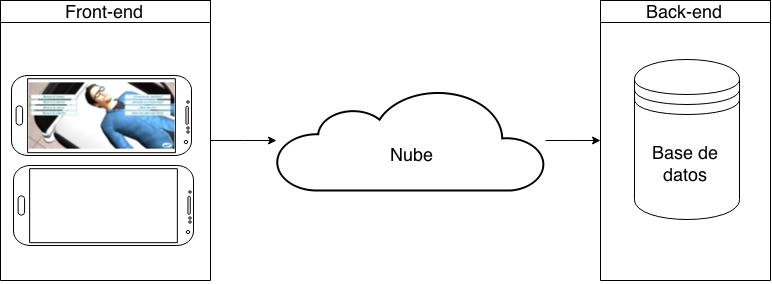
\includegraphics[scale=0.5]{tecnologias/images/full.png}
\end{center}
\caption{Esquema general de los componentes}
\label{fig:componentes}
\end{figure}

La arquitectura se compone de un \textit{front-end}\footnote{El \textit{front-end}
    es la parte de la solución que interactúa con el usuario. Se encarga de
    realizar una simulación, de interpretar las acciones del usuario y evaluar
    el rendimiento del usuario.} que consiste en una aplicación móvil, la cual
es utilizada por los alumnos de enfermería. Los registros de uso del \textit{front-end} son 
almacenados bajo demanda en un servidor
\textit{back-end}\footnote{El \textit{back-end} es la parte de la solución que
    se encarga de almacenar la información de los usuarios y sus acciones dentro
    del \textit{front-end}.}, el cual se encarga de asociar los registros con
los alumnos y almacenarlos de manera persistente.

Así, las herramientas necesarias para el desarrollo se agrupan en:

\begin{itemize}
    \item \textbf{Herramientas de gestión de código}: 
        tecnologías requeridas para gestionar y mantener código.
    \item \textbf{Desarrollo del \textit{front-end}}: 
        tecnologías utilizadas para el desarrollo del videojuego en sí. 
    \item \textbf{Desarrollo del \textit{back-end}}: 
        tecnologías utilizadas para procesar las acciones que los usuarios
        realizan dentro de la solución.
\end{itemize}

La herramienta principal para el desarrollo del front-end es el motor de videojuegos, por lo 
mismo, se debe seleccionar adecuadamente de acuerdo a las características de la solución que 
se desea desarrollar.

A continuación se describen los principales motores de videojuegos utilizados en la actualidad y se 
definen los criterios para seleccionar el más adecuado. Posteriormente se describen las 
tecnologías que son necesarias para la implementación de la solución a más bajo nivel.

\section{Motores de videojuegos}

Para el desarrollo de videojuegos se utilizan programas o herramientas
especializadas en ello llamadas \enquote{Motores de videojuegos}. A continuación
se da una breve introducción de lo que es un motor de videojuego.

El término \enquote{motor de videojuegos} hace referencia a una serie de rutinas
de programación que permiten el diseño, la creación, el desarrollo y la
representación gráfica de un videojuego\cite{videojuego:telechea}.

Además, la gran mayoría de estos motores ofrecen a su vez características y
funciones que facilitan la construcción del videojuego, como el motor físico
(software capaz de realizar \enquote{simulaciones} de ciertos sistemas físicos
como la dinámica de un cuerpo rígido, el movimiento de un fluido o la
elasticidad) o detector de colisiones, sonidos, \textit{scripting}, animaciones,
inteligencia artificial, comunicación a través de redes, \textit{streaming},
administración de memoria, etc\cite{videojuego:telechea}.

El motor de videojuego a utilizar depende de las características que posea el
videojuego que se quiere desarrollar, las cuales fueron descritas en
\ref{chap:requerimientos}. A continuación se da una breve descripción
de los motores de videojuegos más utilizados actualmente, se definen los
criterios de selección y se realiza una comparación entre los mismos, para la
elección del motor de videojuegos que más se adecue a las necesidades de la
solución. Entre los aspectos que son comparados se encuentran la distribución,
librerías, tiendas, licencias, curva de aprendizaje, lenguajes de programación,
entre otros.

\subsection{Unreal Development Kit}

Es la edición gratuita de \textit{Unreal Engine 3}. \textit{Unreal Engine} es el
motor de videojuegos desarrollado por \textit{Epic Games}\cite{unrealengine}.

\Gls{udk} proporciona acceso al motor de juegos 3D y a la herramienta profesional 
que se utiliza en el desarrollo de videojuegos \textit{blockbuster}, visualización 
arquitectónica, el desarrollo de juegos para móviles, modelos 3D, películas digitales 
y más. Utilizando \Gls{udk} se pueden implementar juegos y aplicaciones en
\textit{Windows PC}, \textit{iOS} y \textit{Mac}\cite{unrealengine}.

Posee su propio entorno de desarrollo, las rutinas de programación pueden ser escritas 
en los lenguajes de programación Unreal Script y C++, y una comunidad 
grande donde se puede recurrir. Además soporta formatos de modelos 
3D como fbx, dds, raw y ASE\cite{unrealengine}.

\subsection{Blender Game Engine}

\enquote{Blender Game Engine} es el motor de videojuegos de \textit{Blender Foundation} 
que permite crear aplicaciones 3D interactivas o simulaciones, desarrollado bajo 
la licencia \Gls{gnu}\cite{blender}.

\textit{Blender Game Engine} genera las escenas de forma continua en tiempo real
e incorpora facilidades para la interacción del usuario durante el proceso de
\textit{renderización}, procesa la lógica de sonido, de la física y la 
representación de simulaciones en orden secuencial\cite{blender}.

Posee la posibilidad de exportar en plataformas como
\textit{Windows, Linux y Mac OS}. También incluye básico en desarrollo para 
plataformas Android\cite{blender}.

Posee su propio entorno de desarrollo, las rutinas de programación pueden ser 
escritas en los lenguajes de programación Python y C++, y
una comunidad grande donde se puede recurrir. Además soporta formatos 3D 
como 3ds, dae, fbx, dxf\cite{blender}.

\subsection{CryEngine}

\enquote{CryEngine} es el motor de videojuegos desarrollado por \textit{Crytek}.
Existe una versión gratuita denominada \enquote{CryEngine Free SDK} con todas
las funcionalidades, esta versión esta disponible para su descarga, pero ya ha
sido descontinuada\cite{cryengine:sdk}.

Este motor de videojuegos permite exportar a plataformas como iOS y
Android\cite{cryengine}. Posee su propio entorno de desarrollo, las rutinas de
programación pueden ser escritas en los lenguajes de programación C++ y Lua, y
una comunidad de tamaño moderado donde se puede recurrir. Además sólo soporta
sus propios formatos 3D\cite{cryengine}.

\subsection{ShiVa3D}

\textit{ShiVa3D} es un motor para el desarrollo de videojuegos y aplicaciones 
3D desarrollado por ShiVa Technologies\cite{shiva}.

Un producto relacionado es el \enquote{ShiVa Server}, el cual permite el
desarrollo de aplicaciones multijugador. Las características de este servidor,
incluyen comunicación \textit{VoIp}, etc\cite{shiva}, esta es
una opción interesante para el desarrollo del \textit{backend}.

\textit{ShiVa} puede exportar juegos y aplicaciones a una cantidad variada de 
plataformas, incluyendo móviles como \textit{iOS, Android, BlackBerry y Windows
Phone}, de escritorio como \textit{Windows, Mac OS X y Linux}, los
navegadores web con soporte \textit{Flash y HTML5}, así como consolas como la
\textit{Xbox 360, PlayStation3 y Nintendo Wii}. El \Gls{ide} se ejecuta en
\textit{Windows} y \textit{Mac OS X}\cite{shiva}. 

Posee su propio entorno de desarrollo, las rutinas de programación pueden ser 
escritas en los lenguajes de programación FlowGraph y Lua, y una 
comunidad moderada donde se puede recurrir. Además sólo soporta el formato 
3D, dae\cite{shiva}.


\subsection{Unity3D}

\textit{Unity} es un motor para el desarrollo de juegos,
desarrollado por \textit{Unity Technologies}. Posee una versión pagada 
y una gratuita\cite{unity3d}.

Posee un motor de \textit{renderizado} y un flujo de trabajo para la creación 
de contenido 3D interactivo, además permite mezclar contenido 3D, 2D, sonidos 
y animaciones de manera sencilla\cite{unity3d}.

La versión gratuita permite desarrollar juegos para múltiples plataformas. 
Entre las plataformas móviles soportadas, encontramos a \textit{iOS, Andriod, 
Windows Phone 8, BlackBerry 10}, entre las plataformas de escritorio a 
\textit{Windows, Mac y Linux}, plataformas web como \textit{Internet Explorer,
    Mozzilla Firefox, Google Chrome}\footnote{Requiere un \textit{plugin} para
    el navegador que está disponible para \textit{Windows y Mac}}, y entre
plataformas de consolas a \textit{Xbox 360, Xbox One, Wii, Wii U, Nintendo
    3DS}\cite{unity3d}.

Posee su propio entorno de desarrollo, las rutinas de programación pueden ser 
escritas en los lenguajes de programación \cs{}, UnityScript y Boo, y una 
comunidad grande donde recurrir. Además soporta formatos 3D como fbx, obj, max, 
blend, dae, 3ds, dxf, MB, MA\cite{unity3d}.


%! TEX root = ../main.tex
\section{Selección del motor de videojuego}
\label{sec:seleccion_plataforma}

En esta sección se comparan los motores de videojuegos \textit{Unreal Engine,
    CryEngine, Blender Game Engine, ShiVa3D y Unity3D} según criterios relacionados 
con los requisitos que debe cumplir la solución. Estos criterios son citados a continuación, 
además, se selecciona y justifica la elección del motor de videojuego a utilizarse para 
el desarrollo de la solución propuesta.

\subsection{Criterios de selección}

Para seleccionar el motor de videojuego que se ajuste mejor
a la solución propuesta para facilitar su desarrollo y el cumplimiento de los
requisitos definidos en el capítulo~\ref{sec:requisitos}, se tuvieron en cuenta los
siguientes criterios:

\begin{itemize}
\item Licencia de uso del motor.
\item Plataformas móviles.
\item Lenguajes de programación para el desarrollo.
\item Tienda de librerías y paquetes.
\item Tamaño de la tienda de librerías y paquetes.
\item Representación en \textit{2D} y \textit{3D}.
\item Formatos de modelo \textit{3D} soportados.
\item Soporte de comunidades.
\item Entorno de desarrollo o \Gls{ide}.
\item Licencia del entorno de desarrollo.
\end{itemize}


\subsection{Comparación}

En la tabla~\ref{tab:comparacion_motores_juegos} se comparan los criterios citados 
anteriormente para cada uno de los motores teniendo en cuenta tanto aspectos técnicos 
como de aprendizaje y de uso.

Teniendo en cuenta el resultado de esta comparación y de acuerdo a los
requisitos que debe reunir la solución propuesta se elige a \textit{Unity3D}
como el motor de videojuego ideal para el desarrollo de este trabajo.

Las ventajas principales de esta elección son la cantidad de plataformas móviles
diferentes a las que se puede exportar y distribuir la aplicación ya que uno de
los ejes del trabajo es brindarle movilidad al usuario. Además, \textit{Unity}
posee una gran comunidad de desarrolladores lo cual es importante en los
momentos en el que se poseen dudas que se desean aclarar con rapidez.

\textit{Unity} posee una gran tienda donde se pueden encontrar desde modelos en
tres dimensiones y librerías de sonidos hasta librerías que ofrecen extender o
incluir funcionalidades. 

%\newgeometry{bottom=1cm}


\begin{sidewaystable}
\begin{tabulary}{\textwidth}{L|CCCCCCCC}
\toprule
Característica / Motor &
Unreal Engine          &
CryEngine              &
ShiVa3D                &
Unity3D                &
Blender Game Engine \\
\midrule
Distribución & iOS, soporta otros dispositivos en la versión comercial. &
iOs, Android & iOS, Android, Windows Phone, BlackBerry & Android, WindowsPhone,
iOs, BlackBerry & Soporte en desarrollo para Android \\ 

Tienda de librerias & Sí, en estado Alpha & No, existen tiendas de
terceros & Sí & Sí & Sí \\

Tamaño de tienda & Mediana & Mediana & Pequeña & Grande & Grande \\

Comunidad & Grande & Moderada & Moderada & Grande & Grande \\
Licencia del entorno de desarrollo & Gratuita solo para uso no comercial &
Propietaria & Propietaria & Gratuita para uso no comercial & GPL \\

Formatos soportados & fbx, dds, raw, ASE & Formatos propios & dae & FBX, OBJ,
Max, Blend, dae, 3ds, dxf, MB, MA, etc & 3ds, dae, fbx, dxf, etc \\

Licencia del motor & Versiones antiguas gratuitas para uso no comercial.
& Gratuita solo para uso no comercial & Propietaria, solamente la versión Web es
gratis & Versión limitada gratis, disponible para uso no comercial & GPL \\

Curva de aprendizaje & Compleja & Compleja & Compleja & Sencilla & Compleja \\

Lenguajes de desarrollo & Unreal Script y C++ & C++, Lua & FlowGraph
(propietario) y Lua & \cs{}, UnityScript y Boo & Python y C++ \\

\Gls{ide} & Si, propio & Sí, propio & Sí, propio & Sí, propio & Sí, propio \\
\bottomrule

\end{tabulary}
\caption{Comparacion entre motores de videojuegos}
\label{tab:comparacion_motores_juegos}
\end{sidewaystable}
%\restoregeometry



\section{Entorno de desarrollo de la solución}

Para llevar a cabo el desarrollo completo de la solución se debe recurrir a una 
gran cantidad herramientas, \textit{frameworks}, y recursos. En esta sección se 
describen estas tecnologías.

%En esta sección se describen todos las partes involucradas en el desarrollo de
%la solución propuesta. 

%La solución se compone de dos partes, la primera es la aplicación que los
%usuarios utilizan para realizar las prácticas, denominada \textit{Frontend}, y la segunda
%parte, es un servidor que se encarga de almacenar la información sobre los
%usuarios de la solución y como la utilizan, denominado \textit{Backend}.

%Primeramente se definen las herramientas de gestión de código, pues ellas son
%utilizadas tanto por la solución como por el \textit{backend}, luego se definen
%las herramientas específicas de la creación de la simulación y por último, se
%citan y describen de manera breve las herramientas utilizadas por el
%\textit{backend}.

%La idea detrás de separar la solución en \textit{Frontend} y \textit{Backend} 
%es que ambas partes de la solución se podrán mantener de forma separada sin que 
%el cambio de una afecte el funcionamiento de la otra. 

\subsection{Herramientas de gestión de código}

La gestión del código fuente desarrollado como parte de este trabajo de grado fue realizado
mediante la utilización de la herramienta de control de código fuente
\textit{Git}, \textit{Git} es un software de control de versiones distribuido,
de código abierto bajo la licencia \Gls{gnu}\cite{git}. El proveedor del
servicio \textit{Git} utilizado es \textit{BitBucket}\cite{bitbucket}, el cual
almacena repositorios \textit{Git}, la principal característica y motivación por
la cual se utiliza este servicio es que el mismo permite mantener varios
repositorios privados de manera gratuita\cite{bitbucket}.

\subsection{Desarrollo del \textit{front-end}}

El desarrollo de la solución requiere de una variedad importante de tecnologías
además del motor de videojuego, las herramientas descritas en esta sección complementan al
motor seleccionado y facilitan la creación de contenido.

En primer lugar, se utilizó el \Gls{ide} \textit{Unity Editor} para la creación de las escenas,
el \Gls{ide} \textit{MonoDevelop} y el lenguaje \cs{} para la programación de la
interacción entre los componentes de la solución.

Adicionalmente se utilizaron varias herramientas de diseño para crear
componentes 3D y 2D, \textit{Make Human} es utilizado para la creación de los
pacientes, \textit{3ds Max} permite la creación de objetos como gazas, y otros
elementos utilizados dentro de la solución. En cuanto a los gráficos 2D, se
utilizaron \textit{Photoshop}, y diversas páginas web que proveían contenido
gratuito.

\begin{itemize}

\item \textbf{Unity Editor}

El \Gls{ide} de \textit{Unity} es la herramienta en la se crean los videojuegos
o simulaciones. Este \Gls{ide} importa todos los \textit{asset}\footnote{Un
    \textit{Asset} es un paquete \textit{Unity} que puede contener modelos,
    librerias, sonidos, etc.}. Permite compilar las escenas con los terrenos,
luces, audios, personajes, física, entre otros. Se puede agregar interacción a
través de \textit{scripting}. Además se puede probar y editar en
forma simultánea los videojuegos y desplegarlos en las plataformas
elegidas\cite{unity3d}. 

Este editor es la única herramienta que permite crear escenas en \textit{Unity},
sin embargo, este \Gls{ide}, no permite la edición de código,\footnote{Existen
    \textit{Assets} que permiten la edición de código dentro del \textit{Unity
        Editor}, pero son pagas y de baja reputación} por ello se necesita un
editor externo de código.


\item \textbf{MonoDevelop}

\textit{MonoDevelop} es un \Gls{ide} de código abierto, bajo la licencia
\Gls{gnu} apoyado principalmente por la comunidad \textit{Mono}. Es el \Gls{ide}
utilizado por defecto en el desarrollo de aplicaciones para \textit{Unity3D}, el
mismo soporta varios lenguajes de programación, como \cs{},
\textit{UnityScript}, y \textit{Boo}. Es un \Gls{ide} multiplataforma que
soporta \textit{Windows} al igual que \textit{Unity3D}.

Existen otros editores que pueden ser utilizados para el desarrollo del código
fuente, pero los mismos no cuentan con el mismo nivel de integración y no son
gratuítos.\footnote{\textit{Microsoft Visual Studio} permite el mismo nivel de
    integración que \textit{MonoDevelop} con un \textit{plugin}, pero el mismo
    es de pago durante el desarrollo de la solución}

\item \textbf{\cs{}}

\textit{Unity3D} utiliza versiones limitadas\footnote{La definición del lenguaje
    es la misma, pero las librerías estándar no están completas}de tres
lenguajes de programación: \cs{}, \textit{UnityScript}, y
\textit{Boo}\cite{unity:script}. Estos lenguajes son compilados y orientados a
objetos.

Otra característica interesante es que, por el orden de compilación de los
proyectos \textit{Unity3D}, los archivos \textit{UnityScript} y \textit{Boo} son
compilados antes que los archivos \cs{}, esto provoca que, las clases
\textit{UnityScript} sean utilizables desde \cs{}, lo que no se cumple en el
caso contrario, es decir, las clases \cs{} no son accesibles desde código
\textit{UnityScript} o \textit{Boo}.

Por lo mencionado anteriormente se selecciona a \cs{} como el lenguaje de
implementación. Además, es el lenguaje con más ayuda en línea, y las
librerías no diseñadas específicamente para \textit{Unity3d} pueden ser
utilizadas. Otro factor que influye en la elección es la familiaridad de los
autores con lenguajes similares. 

\item \textbf{Herramientas de diseño}

Las herramientas utilizadas para crear modelos 3D e imágenes 2D son las siguientes:

\begin{itemize}
\item \textbf{MakeHuman}: es un software de código abierto bajo la licencia
    \Gls{agnu} para crear personajes humanos 3D. Es una herramienta diseñada
    para simplificar la creación de seres humanos virtuales utilizando una
    interfaz gráfica de usuario\cite{makehuman}. 
\item \textbf{3ds Max}: es un software privado de modelado 3D, que además posee
    herramientas para animación, simulación y renderización. Esta herramienta
    fue utilizada para crear objetos 3D que no fueran personajes humanos y para
    exportar modelos de un formato a otro que fuera compatible con
    \textit{Unity3D}\cite{3dsmax}.
\item \textbf{Photoshop}: es una herramienta de edición de gráficos 2D de
    \textit{Adobe}, permite la creación y edición de gráficos, es utilizada para
    la creación de iconos, botones y otro contenido 2D que forma parte de la
    solución.
\end{itemize}

\end{itemize}


\subsection{Desarrollo del \textit{back-end}}

Para registrar las actividades del usuario en el front-end, se necesita de un
servidor que almacene los datos de todos los usuarios y las actividades que
estos realizan dentro de la solución.

En la figura~\ref{fig:backend_diagrama} se puede observar en lineas generales
como funciona este servicio, desde el registro de actividades del usuario, la
comunicación con el \textit{back-end}, su posterior traducción y persistencia en
una base datos, así, este servicio debe proveer:

\begin{itemize}
    \item \textbf{Alta disponibilidad}: el servidor debe estar disponible en
        todo momento, cualquier día de la semana y a cualquier hora. Los
        requisitos de accesibilidad son estrictos, pues se necesita que los
        usuarios envíen datos sin inconvenientes cuando crean necesario.
    \item \textbf{Accesibilidad}: el servidor debe poder ser accesible desde
        cualquier red móvil.
    \item \textbf{Bajo costo de comunicación}: la comunicación del usuario con
        el \textit{back-end} debe ser lo menos costosa posible, pues se utilizan
        recursos del usuario.
\end{itemize}

\begin{figure}[H]
\centering
\includegraphics[scale=0.4]{tecnologias/images/backend_diagrama.png}
\caption{Diagrama de la interacción de los usuarios con el \textit{back-end}, se
    puede observar a grandes rasgos, los componentes del sistema y los servicios
    que ofrece.}
\label{fig:backend_diagrama}
\end{figure}

Las tecnologías utilizadas para el desarrollo del \textit{back-end} son:

\begin{itemize}
\item \textbf{\Gls{javaee}}

Para el desarrollo de la aplicación web que almacena los datos se utiliza
\Gls{javaee} en su versión $6$, la misma se utiliza por la familiarización de
los autores con la tecnología y la facilidad que provee para la
realización de servicios web que permitan la interacción con la solución.

\item \textbf{\Gls{rest}}

Para los servicios se utiliza la arquitectura \Gls{rest}, la principal
motivación para utilizar \Gls{rest} es la eficiencia en el uso de la
red\cite{pautasso2008restful}, la cual es también la motivación para la
utilización de \Gls{json}. La implementación del lado del servidor de la
arquitectura \Gls{rest} es \textit{RestEasy}, de parte del \textit{front-end} se utiliza
la implementación por defecto de \textit{Unity3D}.

\item \textbf{PostgresSQL}

El almacenamiento permanente de los datos se logra con la utilización de
\textit{PostgreSQL}, el cual es un motor de bases de datos de código abierto
dirigido por \textit{PostgreSQL Global
    Development Group}. La versión elegida es la $9.1$.

\item \textbf{OpenShift}

A fin de obtener las características necesarias, de alta disponibilidad y
accesibilidad, se utiliza la herramienta de plataforma como servicio de
\textit{RedHat} llamada \textit{OpenShift}, la cual es un producto de código
abierto dirigido por \textit{RedHat}.

Además de dirigir el proyecto, \textit{RedHat} provee un servicio limitado y
gratuito\cite{openshift:pricing}.\footnote{Existen versiones completas del
    producto mantenidas por \textit{RedHat}, las cuales tienen un costo mensual
    y de acuerdo a las funcionalidades utilizadas\cite{openshift:pricing}} Para
esta tesis se utilizo el servicio gratuito con la plataforma \textit{JBoss
    Application Server 7.1} y \textit{PostgreSQL 9.1}.

\end{itemize}

\section{Resumen}

A modo de resumen de las tecnologías utilizadas para el desarrollo de la solución
propuesta se presentan las tablas~\ref{tab:stack_tecnologico_fe} y~\ref{tab:stack_tecnologico_be}.

\begin{table}[H]
\centering
\begin{tabular}{lrr}
\toprule
\textbf{Utilización} & \textbf{Tecnología} & \textbf{Versión} \\
\midrule
Motor de videojuego      & Unity3d         & 4.5 \\
IDE                      & MonoDevelop     & 4 \\
                         & Unity Editor    & 4.5 \\
\midrule
Modelado 3D              & 3ds Max         & 2013 \\
Modelado 2D              & Photoshop       & 14 \\
Modelado de personajes   & MakeHuman       & 1.0 \\

\midrule
Lenguaje de programación & \cs{} \\
Gestión de código fuente & GIT & 1.8 \\
Otras librerías          & NGUI            & 2.7\\
                         & Facebook \\
                         
\bottomrule
\end{tabular}
\caption{Resumen de las tecnologías utilizadas en el \textit{front-end}}
\label{tab:stack_tecnologico_fe}
\end{table}


\begin{table}[H]
\centering
\begin{tabular}{lrr}
\toprule
\textbf{Utilización} & \textbf{Tecnología}  & \textbf{Versión} \\
\midrule
IDE                         & Eclipse & Luna\\
Lenguaje de programación    & Java & 7\\
\midrule
Servidor de aplicaciones    & Jboss & 7 \\
Servidor de base de datos   & PostgreSQL & 9.2 \\
Proveedor de plataforma     & OpenShift \\
\midrule
Gestión de código fuente    & GIT & 1.8\\
Otras librerias             & Java EE & 6\\

\bottomrule
\end{tabular}
\caption{Resumen de las tecnologías utilizadas en el \textit{back-end}}
\label{tab:stack_tecnologico_be}
\end{table}


%! TEX root = ../main.tex
\chapter{Solución}
\label{chap:solucion}

\todo[backgroundcolor=white,inline,caption={Nombres}]{Estos son los nombres
    que pensamos: 
\begin{itemize}
\item evTesai (seria algo como entorno virtual de salud)
\item eve (Entorno virtual de enfemería) (este fue el que mas le gusto)
\end{itemize}}


\observacion{Muchas vueltas en el siguiente párrafo}
En \fixme{capítulos anteriores}{Especificar} se describen los requerimientos que
debe tener la solución para abordar los problemas encontrados en el área de
enfermería dando una propuesta de solución y las tecnologías disponibles para la
implementación de esa solución. En este capítulo se describen los aspectos de la
solución en cuanto a su implementación teniendo en cuenta esos requerimientos y
utilizando esas tecnologías.

La solución consiste en un Juego Serio para dispositivos móviles llamado
\Gls{yave}, el \fixme{cual consiste en ofrecer a los usuarios, en este caso
    alumnos de enfermería}{Los estudiantes}, un medio en el cual puedan realizar
procedimientos de enfermería y cuyo objetivo es servir como herramienta de apoyo
en el aprendizaje.

\Gls{yave}\revisar{Presenta un conjunto de escenas} permite al usuario poder
seleccionar el procedimiento que quiera realizar, dando la posibilidad de
interactuar con un paciente y con una conjunto de objetos que forman parte de
las herramientas requeridas para realizar el procedimiento seleccionado. Además,
contempla la posibilidad de realizar acciones relacionadas a la bioseguridad, y
otros aspectos transversales a la educación de un enfermero.

La solución no sólo le permite al usuario realizar los procedimientos para poner
en practica sus conocimientos sobre los mismos, sino también
\fixme{evaluará}{Tiempo} al usuario, \fixme{dándole}{Mejorar} al final de cada
sesión una puntuación y describiendo los pasos realizados correcta e
incorrectamente, proporcionando información acerca de los puntos incorrectos.

A continuación se detalla las arquitectura general de la solución para 
dar una visión global de la solución, luego se detallan cada una de las partes en 
la que se divide llamadas \emph{Frontend} y \emph{Backend}.

%! TEX root = ../main.tex

\section{Arquitectura general}
\label{sec:solucion}

\observacion{Esta sección 7 deberá empezar con una descripción general (gráfico)
y debe ir explicando parte por parte}

A continuación se describe la arquitectura propuesta para la realización de una
juego serio, \fixme{se utiliza}{} la guía básica definida
por~\cite{pereira2009design} y descrita en~\ref{sec:desarrollo}.

Esta sección se enfoca en los aspectos técnicos de la creación del juego serio,
las competencias básicas relacionadas con la educación (segundo paso de la guía
descrita en~\ref{sec:desarrollo}) se definieron en las
secciones~\ref{sec:glasgow} y~\ref{sec:hemocultivo}.

La solución se basa en escena\fixme{s, u}{}na escena es un procedimiento definido
en~\ref{sec:seleccion_escenas}, cada escena tiene sus propias entidades, eventos
y requisitos específicos. \fixme{Adicionalmente existe otra escena denominada
Inicio que es la escena donde se inicia la solución.}{?}
%Inicio estaba en un \enquote

\observacion{Grafo de la arquitectura? Esta un poco desordenado}

Adicionalmente la solución cuenta con pantallas, que son vistas donde el usuario
puede seleccionar varias opciones, a continuación se describe el funcionamiento
global de la solución y la transición entre las escenas, pantallas y diversas
opciones existentes. Posteriormente se define como se interactúa con el entorno,
y a continuación se evalúa al alumno durante su experiencia con la solución.

\subsection{Flujo de la solución}

\observacion{Mejorar siguiente parrafo}
La solución consiste varios escenarios, y cada escenario, \fixme{existen}{Se
    presenta?} varias pantallas que muestran información relevante de acuerdo a
la situación de la simulación, la figura~\ref{fig:grafo_estados} es una
representación abstracta de este flujo de acciones disponibles dentro de la
solución.

\begin{figure}[H] 
\centering 
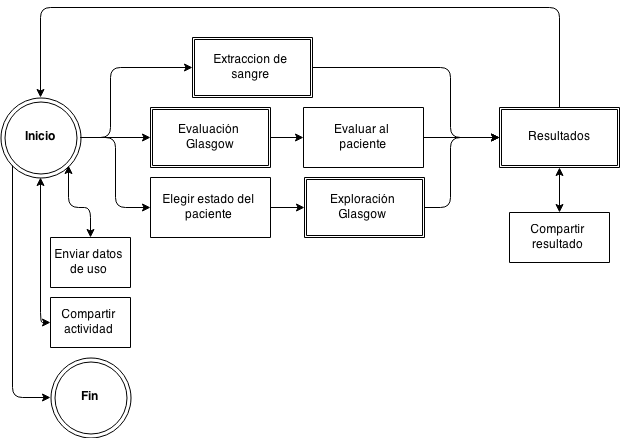
\includegraphics[scale=0.5]{solucion/images/grafo_escenas.png}
\caption{Diagrama de navegación entre los distintos escenarios y pantallas
    disponibles en la solución.}
\label{fig:grafo_estados}
\end{figure}

 
La figura~\ref{fig:grafo_estados} muestra que la solución empieza con una escena
denominada \emph{Inicio}. En la pantalla \emph{Inicio} se observa el escenario y 
opciones, que conducen a los escenarios \emph{Extracción de Sangre} y
\emph{Glasgow}. Otras opciones incluidos en el escenario \emph{Inicio} son
\begin{enumerate*}[label=\itshape\alph*\upshape)]
\item enviar datos de uso al \emph{backend},
\item iniciar sesión en el \emph{Facebook}, y,
\item salir de la simulación.
\end{enumerate*}


\fixme{El escenario \emph{Extracción de Sangre} finaliza al presionar la opción
\emph{Finalizar Partida} y luego se muestra la pantalla \emph{Resultados}, con
información de retroalimentación y la opciones de compartir resultado y volver
a la escena \emph{Inicio}.}{Finalizar }

Para iniciar el escenario \emph{Glasgow} existen dos caminos:
\begin{enumerate}
\item \textbf{Explorar}: desde la escena \emph{Inicio} se elige la opción \emph{Explorar
        Glasgow} en ese momento se muestra la pantalla \emph{Elegir estado del
        paciente}, donde se personaliza el estado del paciente y luego se inicia
    la escena. La escena finaliza con la opción \emph{Finalizar Partida} y se
    muestra la pantalla \emph{Resultados}.
\item \textbf{Evaluar}: desde la escena \emph{Inicio} se elige la opción \emph{Evaluar
        Glasgow} y se inicia la escena \emph{Glasgow} con un estado del paciente
    aleatorio.
    Al finalizar la escena, se muestra la pantalla \emph{Evaluar al paciente}
    donde se permite elegir el estado del paciente, y luego se pasa a la
    pantalla \emph{Resultados}
\end{enumerate}

Finalmente, en la pantalla \emph{Resultados} se permite compartir resultado y
volver a la escena \emph{Inicio}.

Todos los escenarios son utilizados de manera similar, la interacción con la
escena es siempre la misma.

\subsection{Transformaciones del punto de vista del usuario}

El usuario se desenvuelve en un entorno de tres dimensiones, en el cual realiza
las actividades relacionadas a la práctica, se distinguen dos tipos de acciones
principales que el usuario puede realizar:

\begin{itemize}
    \item \textbf{Alejamiento o acercamiento}: es el acto de acercar o alejar la
        cámara, y por consiguiente al usuario del paciente. Se realiza
        utilizando dos dedos, para realizar un acercamiento, mientras se
        mantiene presionada la pantalla con ambos dedos, se procede a alejar un
        dedo del otro, para realizar un alejamiento, se debe acercar ambos
        dedos.
    \item \textbf{Rotación}: se refiere al movimiento de rotación alrededor de
        un foco, que en ambas escenas es el paciente, para realizarla, se utiliza
        un dedo, y se mueve el dedo en cualquier dirección, la cámara, se moverá
        en la dirección contraria.
\end{itemize}

\subsection{Evaluación del usuario}
\label{sec:eca_impl}

\todo[backgroundcolor=white,inline,caption={Pregunta}]{Si esto esta flotando acá
    es por que no sabemos donde podemos poner los detalles de implementación del
    Motor, no se ponen en la parte de extracción de sangre para mantener la
    consistencia con glasgow.}

En la sección~\ref{sec:eca} se describen los \Gls{eca}, y los mismos son
utilizados para poder realizar la evaluación del alumno en la solución.

Definir si las acciones de un usuario son correctas utilizando un motor
\Gls{eca} es sencillo teniendo en cuenta que sólo se deben definir un
conjunto de acciones que se deben realizar, y agregar una acción que verifica si
los pasos realizados fueron los correctos.

Se describe como se crean las reglas, de manera a explicar como son utilizadas
para la evaluación de las acciones realizadas por el usuario.

La definición de las reglas se realiza de la siguiente forma:

\begin{algorithm}[H]
\caption{Creación de regla de verificación de calzado de guantes}
\label{alg:rule_guante}
\lstset{style=sharpc}
\begin{lstlisting}
Rule.New().
     When(``enfermero.guantes.calzar'').
     Then(enviroment => enviroment.
            estadoPaciente.TieneManosLimpias()).
\end{lstlisting}
\end{algorithm}

La regla del algoritmo~\ref{alg:rule_guante} controla que el estudiante ha
realizado la acción \enquote{Calzarse los guantes}, y en ese momento tenga las
manos limpias.

\subsubsection{Estados de una regla}
\observacion{Hacer referencia a la figura 7.2 o mover adelante (la figura del
    ciclo de vida)}

Una regla puede estar en uno de los siguientes estados:

\begin{enumerate}
\item \textbf{BEGIN} Es una regla que recién fue creada, no realiza ninguna
	acción.
\item \textbf{WAITING\_FOR\_RULE:} Es un estado en el que esta esperando que otras reglas
	sean lanzadas. En este estado, es un suscriptor de las reglas por la que
	espera, y no forma parte del ciclo de ejecución del motor de reglas.
\item \textbf{WAITING\_FOR\_EVENT:} Es un estado en el que esta escuchando que sean
	lanzados los eventos a los que escucha, este es el estado principal. En
	este estado, es un suscriptor de los eventos por los que espera, y no
	forma parte del ciclo de ejecución del motor de reglas.
\item \textbf{WAITING\_FOR\_CONDITION:} La regla ya no espera por ningún evento y las
	reglas de las que depende ya han sido lanzadas, se verifica cada cierto
	tiempo si el entorno cumple con una condición definida. 
\item \textbf{FINISH:} Estado final de una regla.
\end{enumerate}

\begin{figure}
\centering
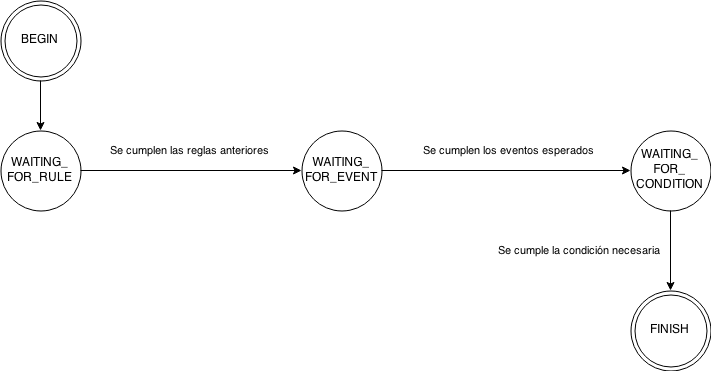
\includegraphics[width=12cm]{solucion/images/rules_flow.png}
\caption{Ciclo de vida de una regla}
\label{fig:rule_flow}
\end{figure}

En la figura~\ref{fig:rule_flow} se observa la evolución de una regla, es
importante notar que una regla solo puede avanzar en este flujo.

\subsubsection{Motor de ejecución}

Un motor de reglas \gls{eca}, requiere de un proceso que evalúe constantemente
las reglas para verificar si las mismas deben ser lanzadas o
no\cite{bailey2004event,galton2002two}, un algoritmo comúnmente utilizado para
realizar la verificación es el algoritmo de \enquote{RETE}\revisar{Tener el
    algoritmo en la presentación, como anexo}\cite{de2001eca}, la cantidad de
reglas definidas, y la no dependencia circular entre ellas, hace innecesario la
implementación de tal algoritmo\cite{de2001eca}. 

De acuerdo a la descripción dada en~\ref{sec:eca_ejecucion}, la propuesta
implementada utiliza una ejecución inmediata, principalmente por la sencillez
de las reglas, es decir, las reglas no realizan un proceso complejo, solamente
controlan el estado del entorno y lo validan.

Además, la ejecución inmediata es importante por que el entorno no sufre
modificaciones entre el evento lanzado y la ejecución de la regla, según
\cite{bailey2004event}, este es el factor más importante para determinar el tipo
de ejecución deseado.

El motor de reglas actúa sobre aquellas reglas en estado
\emph{WAITING\_FOR\_CONDITION} e invoca al procedimiento que se encarga de
validar si la regla puede ser activada (el procedimiento es único por cada
regla), si el mismo determina que la regla puede ser lanzada, el motor ejecuta
la acción de la regla y modifica el estado de la regla a \emph{FINISH}.

%A continuación, se describen todos los escenarios, primeramente se da una
%descripción general de los escenarios y se procede a explicar los detalles de
%los mismos, incluyendo las entidades, eventos y acciones que pueden ser
%realizados en el mismo.

\section{Front-end}

En esta sección se detallan cada uno de los escenarios con los que cuenta 
la solución, incluyendo la retroalimentación y el registro de las actividades del 
usuario.

Las descripciones a continuación están agrupadas por los escenarios principales.

\subsection{Pantalla de inicio}

La solución se inicia con un escenario que está inspirado en el laboratorio de
enfermería del \Gls{iab}, es la primera experiencia que tiene el usuario al
utilizar la misma, sirve como un menú principal, desde este punto todas las
opciones son accesibles para el usuario como se puede observar en la
figura~\ref{fig:pantalla_inicio}, este escenario es denominado~\emph{Inicio}.

Al instalar la solución se muestra una pequeña ventana solicitando el número de
teléfono del usuario, se utiliza esta información como un identificador del
usuario para asociar la información del mismo con un alumno en
particular.

\begin{figure}[H] 
\centering 
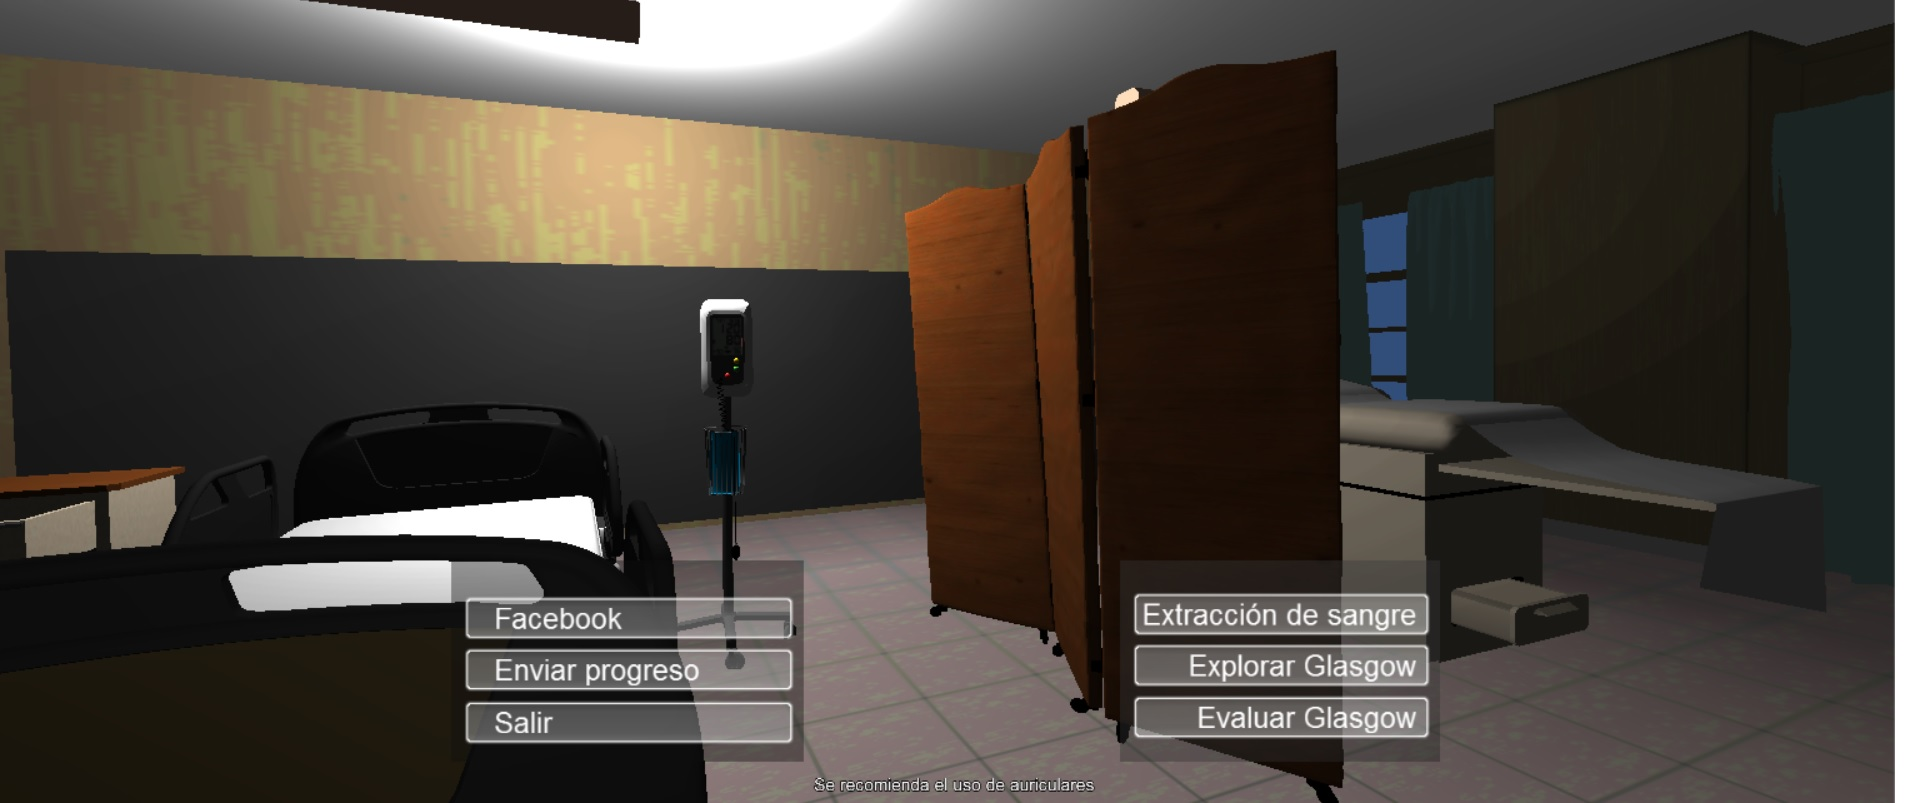
\includegraphics[width=10cm]{solucion/images/pantalla_inicio.jpg}
\caption{Pantalla de inicio de la solución con todas las opciones disponibles.}
\label{fig:pantalla_inicio}
\end{figure}

La sala de hospital mostrada como fondo en la figura~\ref{fig:pantalla_inicio}
es la que se utiliza como escenografía principal en las escenas de los
procedimientos. Mientras se muestran las opciones, se ejecuta una animación que
recorre el escenario mostrando los detalles importantes, como la camilla, el
lector de estadísticas vitales, y demás elementos del escenario.

Las opciones disponibles en la pantalla de inicio son:

\begin{itemize}
\item \enquote{Enviar Progreso}: esta función envía toda la información
    acerca de la actividad que el usuario realizó en la aplicación a un servidor
    \emph{back-end} que se encarga de almacenar estos datos.
\item \enquote{Salir de la simulación}: esta función permite salir de la
    aplicación.
\item Botón \enquote{Facebook}: esta función permite al usuario ingresar a su
    cuenta de Facebook.
\item \enquote{Extracción de sangre}: esta función permite ingresar a la
    escena correspondiente al procedimiento de venopunción 
    permitiendo al usuario jugar una nueva partida.
\item \enquote{Explorar Glasgow}: esta función permite ingresar a la
    escena correspondiente al procedimiento para explorar las reacción de un
    paciente con un diagnóstico específico de la escala de Glasgow permitiendo
    al usuario jugar una nueva partida.
\item \enquote{Evaluar Glasgow}: esta función permite ingresar a la escena
    correspondiente al procedimiento de valoración de la
    escala de Glasgow para un paciente con estado aleatorio permitiendo al
    usuario jugar una nueva partida.
\end{itemize}


\subsection{Venopunción}

Al seleccionar el procedimiento de venopunción o extracción de sangre, en la pantalla de inicio,  
la aplicación inmediatamente muestra el escenario del procedimiento como se puede 
observar en la figura~\ref{fig:hemocultivo_principal}. 

\begin{figure}[H] 
\centering 
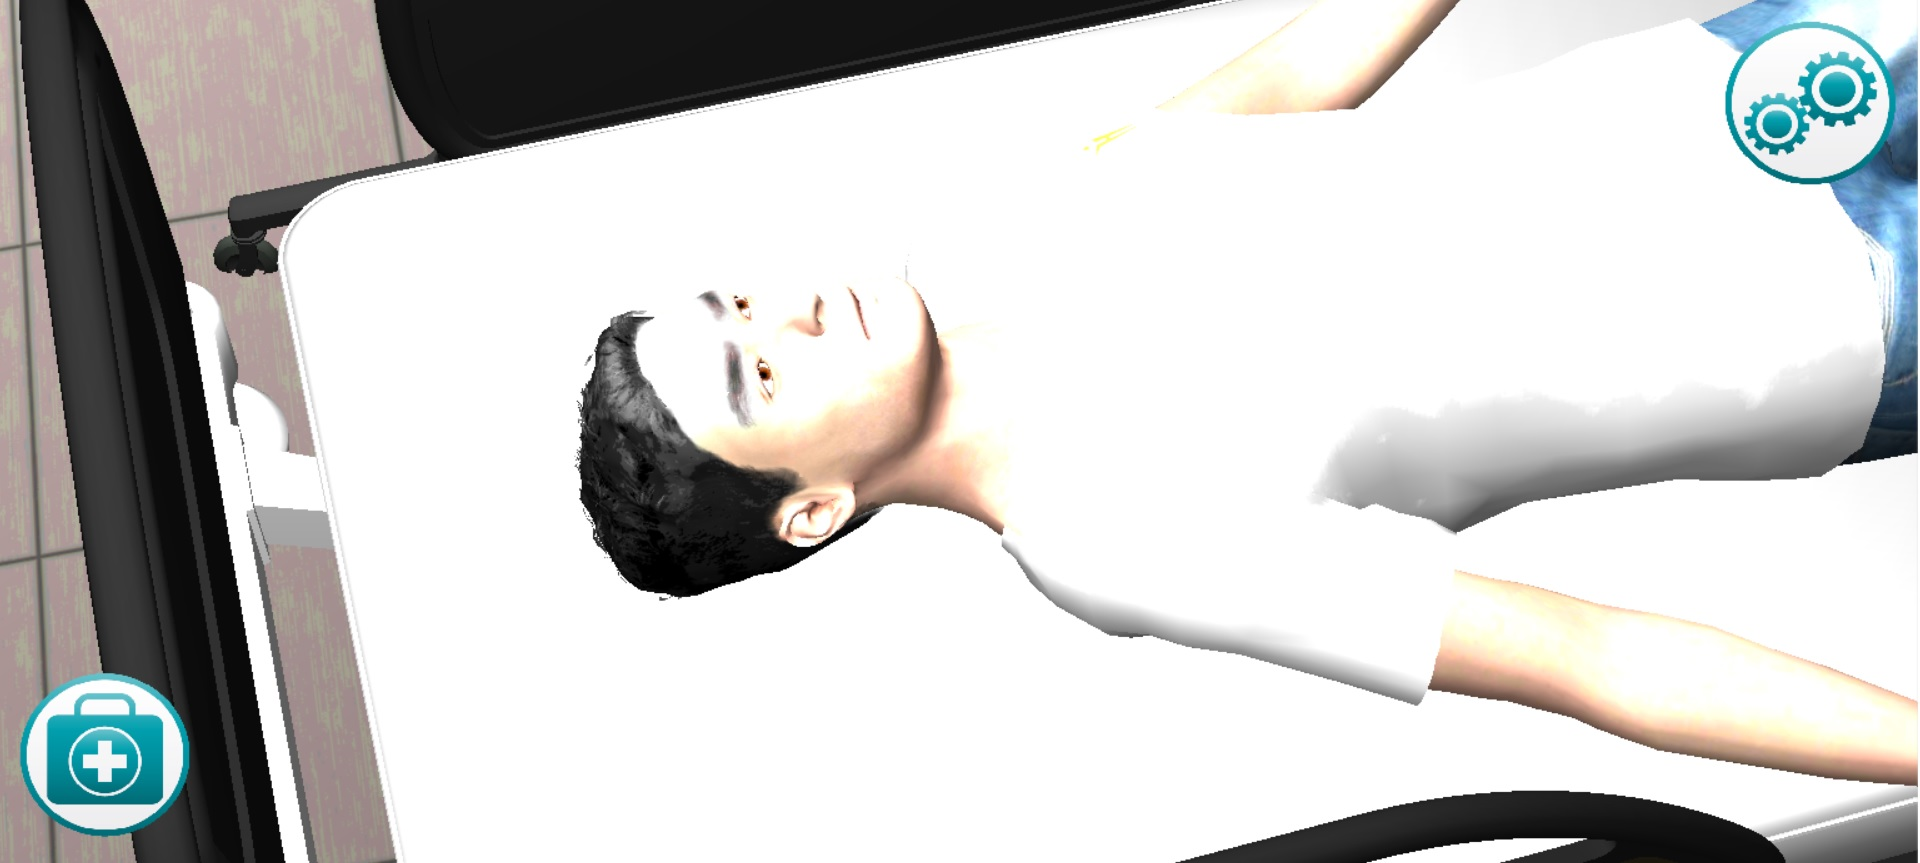
\includegraphics[width=10cm]{solucion/images/hemocultivo_principal.jpg}
\caption{Pantalla principal de la escena del procedimiento de extracción de sangre.}
\label{fig:hemocultivo_principal}
\end{figure}

La posición inicial de la cámara se ubica en un ángulo donde se puedan ver 
bien los brazos del paciente para facilitar al usuario la realización del 
procedimiento.

A continuación se detallan cada una de las opciones y formas disponibles de
interactuar con el escenario del procedimiento.


\subsubsection{Entidades}

Existen dos entidades principales, cada entidad mantiene un estado independiente 
de la otra. Estas entidades son:

\begin{itemize}

\item \textbf{Paciente:} es una entidad con estado complejo, el cual es
    constantemente modificado por las acciones del usuario, en resumen, la
    información que contiene el paciente es:
    \begin{itemize}
        \item Jeringas\footnote{No se limita la cantidad de jeringas que un
                paciente pueda tener insertadas en un momento dado.}.
        \item Estado de las manos (abiertas o cerradas).
        \item Torniquetes.
        \item Zonas esterilizadas.
        \item Zonas presionadas.
    \end{itemize}

\item \textbf{Usuario:} mantiene un estado en todo momento del cual dependen sus
    acciones. Por ejemplo, si la mano del enfermero no está esterilizada,
    cualquier interacción con el paciente provocará que el paciente se
    contamine. La información que contiene la entidad usuario es:

    \begin{itemize}
    \item Estado de las manos.
    \item Estado de la vestimenta (guantes, bata, tapaboca y gorro).
    \item Elemento en uso.
    \end{itemize}
\end{itemize}

\subsubsection{Interacción con la interfaz de usuario}

La interfaz principal de este escenario posee dos menús como se indica en la
figura~\ref{fig:hemocultivo_gui} con los números $1$ y $2$, las opciones dentro
cada menú poseen una imagen intuitiva que representa la función que realizan. Al
menú número 1 lo llamaremos \emph{Elementos} y al número 2 \emph{Opciones}.

\begin{figure}[H]
\centering
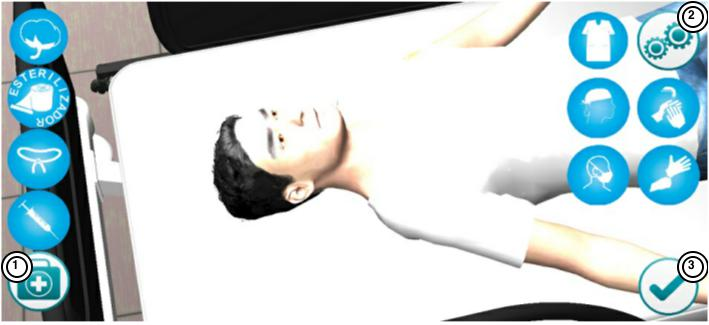
\includegraphics[width=10cm]{solucion/images/hemocultivo_menus.jpg}
\caption{Vista de la interfaz principal del escenario \emph{Extracción de
        sangre}, con todas las opciones desplegadas.}
\label{fig:hemocultivo_gui}
\end{figure}

Adicionalmente, existen dos tipos de indicadores mostrados en la
figura~\ref{fig:hemocultivo_seleccion}. El tipo de indicador marcado con el número $1$
representa el elemento actualmente seleccionado y el tipo de indicador marcado
con el número $2$ representa al estado actual del usuario o enfermero en cuanto a
aspectos de bioseguridad referentes a vestimentas de protección personal.

\begin{figure}[H]
\centering
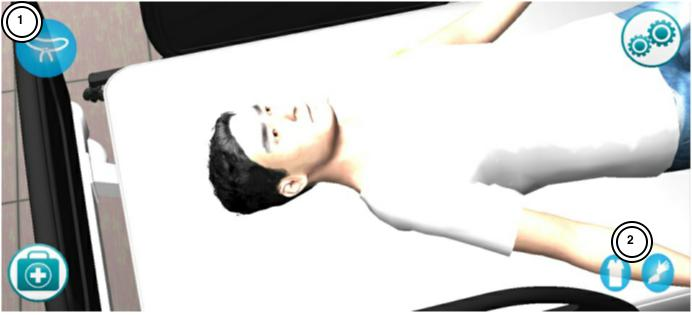
\includegraphics[width=10cm]{solucion/images/hemocultivo_seleccion.jpg}
\caption{Indicadores de selección de elementos y de estado de usuario o enfermero.}
\label{fig:hemocultivo_seleccion}
\end{figure}

\begin{itemize}
\item \textbf{Menú de opciones}

Cuando el usuario presiona el menú \emph{Opciones} se le muestra las distintas acciones que puede
realizar en cuanto a aspectos de bioseguridad, todos los botones
afectan al estado del usuario o enfermero. %Con excepción del lavado de manos,
%las opciones disponibles representan el hecho de ponerse/sacarse los guantes, el
%tapaboca, el gorro y la bata, esto se da seleccionando/deseleccionando estas
%opciones. 
Además se brinda la opción de finalizar la partida con el botón
indicado en la figura~\ref{fig:hemocultivo_gui} con el número $3$.

\item \textbf{Menú de elementos}

En el menú \emph{Elementos} se despliegan opciones que representan a los
elementos que se utilizan para realizar el procedimiento, una vez presionado un
elemento queda seleccionado (simulando que es la herramienta que el enfermero
tiene en la mano en ese momento), sólo un elemento puede ser seleccionado a la
vez. Si el mismo botón se vuelve a presionar inmediatamente después de haber
sido presionado, el elemento se des-selecciona (simulando que el enfermero dejó
la herramienta). Los elementos disponibles están enumerados en la
figura~\ref{fig:hemocultivo_elementos} y son los siguientes:


\begin{figure}[H]
\centering
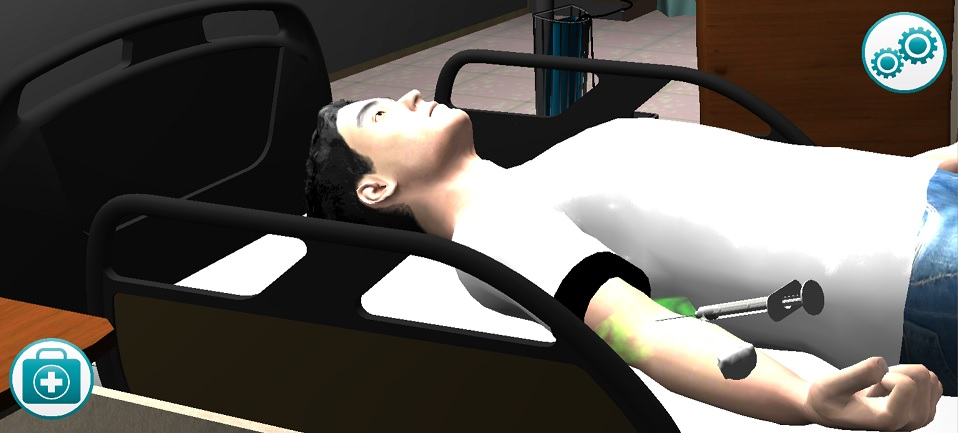
\includegraphics[width=10cm]{solucion/images/hemocultivo_elementos.jpg}
\caption{Interfaz con los elementos en el paciente.}
\label{fig:hemocultivo_elementos}
\end{figure}


\begin{enumerate} 
    
\item \textbf{Torniquete}: es el primer elemento que se debe usar, para
    utilizarlo, se debe presionar una zona del brazo del paciente, en ese
    momento, el torniquete aparece en ese lugar, para extraerlo, se debe
    presionar el torniquete y elegir la opción extraer en un menú que aparecerá
    inmediatamente.

\item \textbf{Esterilizador}: es un elemento que se utiliza para realizar la
    higienización del punto de punción, para utilizarlo se debe presionar
    cualquier zona del brazo del paciente, a continuación aparece una gaza, la
    cual debe ser agitada con un dedo durante un segundo para que se cree una
    zona estéril, la zona estéril creada, es visible a través de una cápsula.

\item \textbf{Jeringa}: es el elemento utilizado para realizar la extracción, su
    utilización es similar a la del \emph{Torniquete}.

    A través de un menú contextual, se ofrece la posibilidad de realizar un
    acercamiento, como se observa en la
    figura~\ref{fig:hemocultivo_jeringa_zoom}, en la vista ampliada. Se puede
    realizar la extracción de sangre utilizando dos dedos, con el primero se
    presiona el tambor y con el segundo dedo se extrae el émbolo\footnote{El
        tambor es la parte de la jeringa que almacena el fluido, mientras que el
        émbolo es la parte que se utiliza para presionar o succionar el fluido}.
    
\item \textbf{Algodón}: el algodón se utiliza para presionar una zona que
    recientemente fue punzada, para utilizar este elemento, basta con presionar
    el brazo del paciente durante un segundo.

\end{enumerate}

\begin{figure}[H]
\centering 
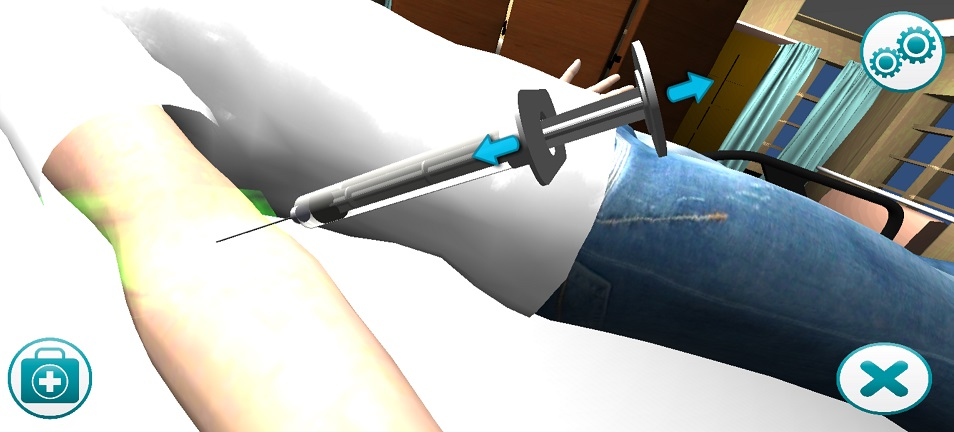
\includegraphics[width=10cm]{solucion/images/hemocultivo_jeringa_ampliada.jpg}
\caption{Vista de la jeringa ampliada, facilitando la extracción de sangre. Se
    agregan flechas azules para facilitar la comprensión de cómo se extrae
    sangre.}
\label{fig:hemocultivo_jeringa_zoom}
\end{figure}


Para la utilización de los elementos, existe un menú contextual\footnote{Un menú
    que se despliega al presionar un elemento, es contextual pues varía de
    acuerdo al elemento seleccionado.}, que lista las opciones disponibles por
elemento, como se observa en la figura~\ref{fig:hemocultivo_torniquete_cm}.

\begin{figure}[H]
\centering
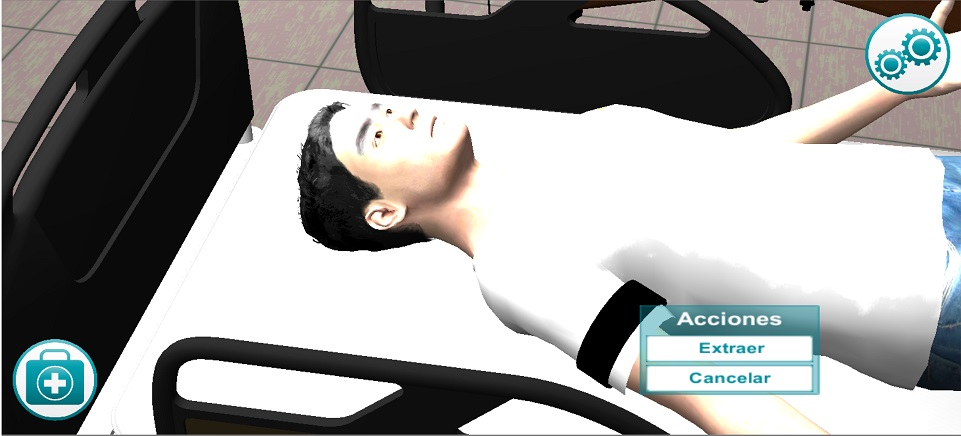
\includegraphics[width=10cm]{solucion/images/hemocultivo_contextual.jpg}
\caption{Menú contextual del elemento torniquete.}
\label{fig:hemocultivo_torniquete_cm}
\end{figure}


\item \textbf{Menú de comandos de voz}

Por último, la solución también cuenta con un menú que presenta una serie de órdenes 
de voz como se observa en la figura~\ref{fig:hemocultivo_voz_gui}. Este menú se 
	activa y se muestra en pantalla cuando la solución detecta que el usuario ha 
	hablado. Las opciones disponibles son las siguientes:
	
	\begin{itemize}
	\item Explicar procedimiento.
	\item Abrir la mano izquierda.
	\item Abrir la mano derecha.
	\item Cerrar la mano izquierda.
	\item Cerrar la mano derecha.
	\end{itemize}
	
	Estas opciones, a excepción de \emph{Explicar procedimiento}, provocan que el 
	paciente realice la petición realizada. De esta manera se simula una conversación 
	entre el usuario y el paciente.
	
	\begin{figure}[H]
	\centering
	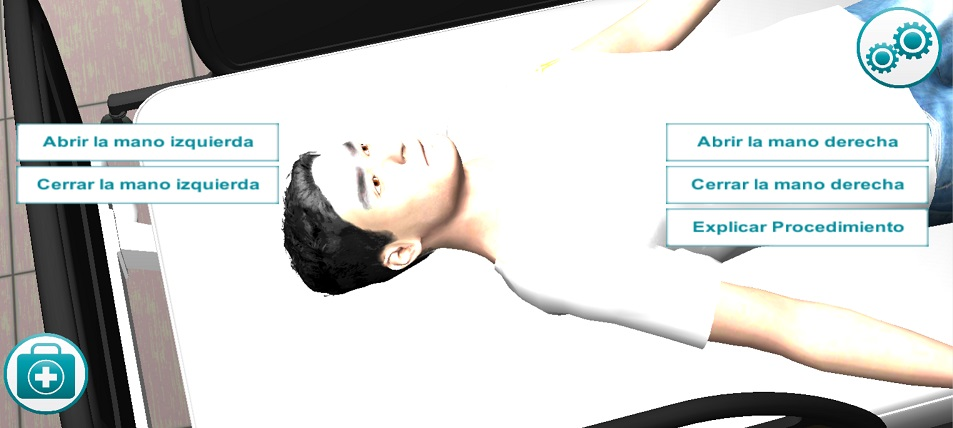
\includegraphics[width=10cm]{solucion/images/hemocultivo_comando_voz.jpg}
	\caption{Opciones mostradas al detectar sonido en la escena de extracción
    de sangre.}
	\label{fig:hemocultivo_voz_gui}
	\end{figure}

\end{itemize}

%\observacion{Pulir el párrafo siguiente}








%\subsubsection{Acciones}
%\observacion{Sean consistentes con las terminologías}
%
%Los usuarios pueden interactuar con el paciente virtual de tres formas, por
%\emph{comandos de voz} que simulan una conversación entre el paciente y
%enfermero, por \emph{las opciones}, que engloban las acciones que puede realizar un
%enfermero en cuanto a bioseguridad, y por \emph{los elementos} que son las
%herramientas que puede utilizar el enfermero durante un procedimiento.
%
%\begin{itemize}
%\item{\textbf{Comando de voz}}
%
%	Se implementa un menú que presenta una serie de órdenes de voz como se observa en la figura~\ref{fig:hemocultivo_voz_gui}. Este menú se 
%	activa y se muestra en pantalla cuando la solución detecta que el usuario ha 
%	hablado. Las opciones disponibles son las siguientes:
%	
%	\begin{itemize}
%	\item Explicar procedimiento.
%	\item Abrir la mano izquierda.
%	\item Abrir la mano derecha.
%	\item Cerrar la mano izquierda.
%	\item Cerrar la mano derecha.
%	\end{itemize}
%	
%	Estas opciones, a excepción de \emph{Explicar procedimiento}, provocan que el 
%	paciente realice la petición realizada. De esta manera se simula una conversación 
%	entre el usuario y el paciente.
%
%\begin{figure}[H]
%\centering
%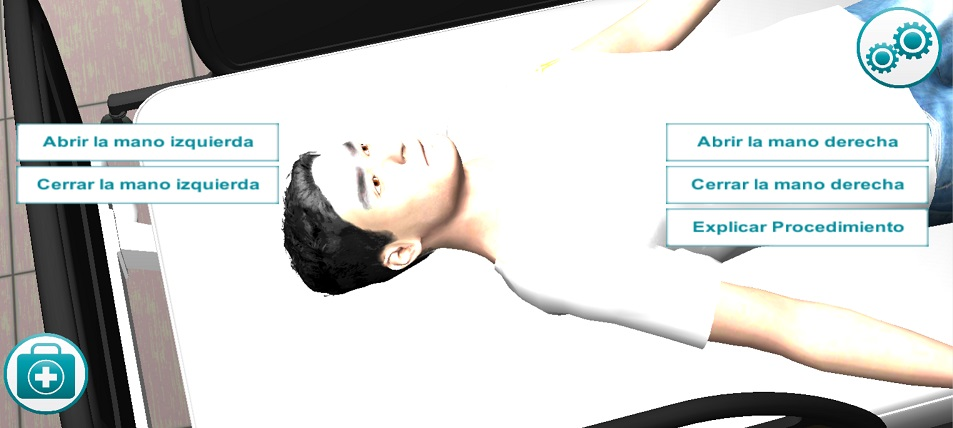
\includegraphics[width=10cm]{solucion/images/hemocultivo_comando_voz.jpg}
%\caption{Opciones mostradas al detectar sonido en la escena de extracción
%    de sangre.}
%\label{fig:hemocultivo_voz_gui}
%\end{figure}
%
%
%
%\item{\textbf{Opciones}}
%
%Las \emph{Opciones} representan las acciones que puede realizar el usuario haciendo uso de las opciones  
%disponibles en el menú indicado por el número 2 en la figura~\ref{fig:hemocultivo_menus}. Estas 
%opciones afectan al estado de la entidad \emph{enfermero} y representan a los aspectos de 
%bioseguridad como el lavado de manos, en calzado de guantes, entre otros.
%
%\begin{figure}[H]
%\centering
%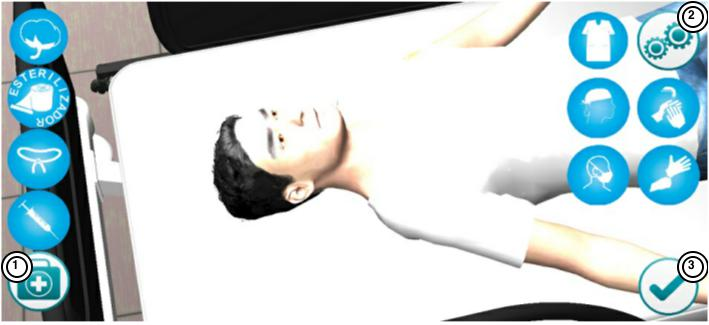
\includegraphics[width=10cm]{solucion/images/hemocultivo_menus.jpg}
%\caption{Menús de la escena principal del procedimiento de venopunción.}
%\label{fig:hemocultivo_menus}
%\end{figure}
%
%%Las \emph{Opciones} son aquellas acciones que puede realizar el usuario y afectan
%%únicamente al paciente. Representan a los aspectos de bioseguridad, es decir,
%%acciones como lavarse las manos, calzarse guantes, gorro, bata y tapaboca.
%%
%%Estas opciones afectan al estado de la entidad \emph{enfermero}.
%
%\item{\textbf{Elementos}}
%
%Los \emph{Elementos} representan las herramientas que utiliza un enfermero
%durante el procedimiento, un solo elemento puede ser utilizado en cualquier
%momento. Las opciones disponibles se pueden ver en el menú marcado por el número 1 
%en la figura~\ref{fig:hemocultivo_menus}. 
%
%
%%\observacion{Desconectado?}
%%\observacion{Falta una intro a todo esto (se refiere a los elementos, y a la
%%    descripción de la imagen~\ref{fig:hemocultivo_voz_gui})}
%\begin{figure}[H]
%\centering
%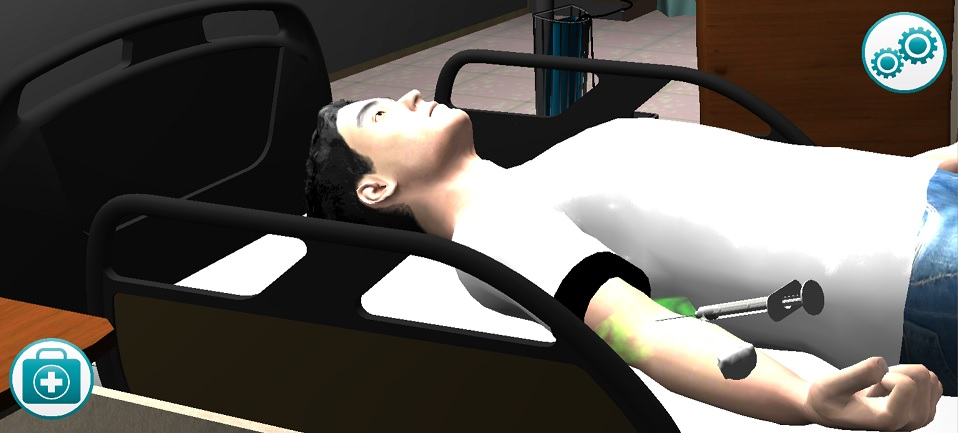
\includegraphics[width=10cm]{solucion/images/hemocultivo_elementos.jpg}
%\caption{Interfaz con los elementos en el paciente.}
%\label{fig:hemocultivo_elementos}
%\end{figure}
%
%Los elementos enumerados en la figura~\ref{fig:hemocultivo_elementos}, son:
%
%\begin{enumerate}
%\item \textbf{Torniquete}: es el primer elemento que se debe usar, para
%    utilizarlo, se debe presionar una zona del brazo del
%    paciente, en ese momento, el torniquete aparece en ese lugar, para
%    extraerlo, se debe presionar el torniquete y elegir la opción extraer en un menú 
%    que aparecerá inmediatamente.
%
%\item \textbf{Esterilizador}: es un elemento que se utiliza para realizar la
%    higienización del punto de punción, para utilizarlo se debe presionar
%    cualquier zona del brazo del paciente, a continuación aparece una gaza, la
%    cual debe ser agitada con un dedo durante un segundo para que se cree una
%    zona estéril, la zona estéril creada, es visible a través de una cápsula.
%
%\item \textbf{Jeringa}: es el elemento utilizado para realizar la extracción, su
%    utilización es similar a la del \emph{Torniquete}.
%
%    A través de un menú contextual, se ofrece la posibilidad de realizar un
%    acercamiento, como se observa en la figura~\ref{fig:hemocultivo_jeringa_zoom}, 
%    en la vista ampliada. Se puede realizar la extracción de sangre utilizando dos dedos, 
%    con el primero se presiona el tambor y con el segundo dedo se extrae el émbolo\footnote{El
%    tambor es la parte de la jeringa que almacena el fluido, mientras que el
%    émbolo es la parte que se utiliza para presionar o succionar el fluido}.
%    
%\item \textbf{Algodón}: el algodón se utiliza para presionar una zona que
%    recientemente fue punzada, para utilizar este elemento, basta con presionar
%    el brazo del paciente durante un segundo.
%
%\end{enumerate}
%
%
%\begin{figure}[H]
%\centering 
%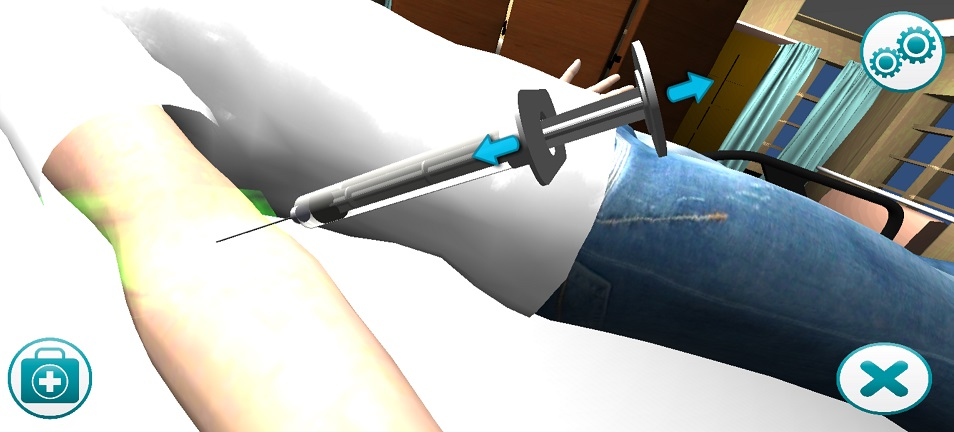
\includegraphics[width=10cm]{solucion/images/hemocultivo_jeringa_ampliada.jpg}
%\caption{Vista de la jeringa ampliada, facilitando la extracción de sangre. Se
%    agregan flechas azules para facilitar la comprensión de cómo se extrae
%    sangre.}
%\label{fig:hemocultivo_jeringa_zoom}
%\end{figure}
%
%\end{itemize}

\subsubsection{Evaluación al usuario}

Para realizar la evaluación del usuario en el procedimiento de \emph{Venopunción} 
se utiliza un motor de \Gls{eca}, las características de estos motores están descritas 
en la sección~\ref{sec:eca}.

Definir si las acciones de un usuario son correctas utilizando un motor 
\Gls{eca} es sencillo teniendo en cuenta que sólo se deben definir un
conjunto de acciones que se deben realizar, y agregar una condición que verifica si
los pasos realizados fueron los correctos.

%Se describe como se crean las reglas, de manera a explicar como son utilizadas
%para la evaluación de las acciones realizadas por el usuario.

A continuación se muestra como se definen las reglas para la validación de las acciones realizadas 
por el usuario.

\begin{algorithm}[H]
\caption{Creación de regla de verificación de calzado de guantes}
\label{alg:rule_guante}
\lstset{style=sharpc}
\begin{lstlisting}
Rule.New().
     When(``enfermero.guantes.calzar'').
     Then(enviroment => enviroment.
            estadoPaciente.TieneManosLimpias()).
\end{lstlisting}
\end{algorithm}

La regla del algoritmo~\ref{alg:rule_guante} controla que el estudiante ha
realizado la acción \enquote{Calzarse los guantes}, y en ese momento tenga las 
manos limpias.

El ciclo de vida de una regla, como se observa en la figura~\ref{fig:rule_flow},
se compone de los siguientes estados:
\begin{enumerate}
\item \textbf{BEGIN:} es una regla que recién fue creada, no se realiza ninguna
	acción.
\item \textbf{WAITING\_FOR\_RULE:} es un estado en el que esta esperando que otras reglas
	sean lanzadas. En este estado, es un suscriptor de las reglas por la que
	espera, y no forma parte del ciclo de ejecución del motor de reglas.
\item \textbf{WAITING\_FOR\_EVENT:} es un estado en el que está esperando que sean
	lanzados los eventos a los que está escuchando, este es el estado principal. En
	este estado, es un suscriptor de los eventos por los que espera, y no
	forma parte del ciclo de ejecución del motor de reglas.
\item \textbf{WAITING\_FOR\_CONDITION:} la regla ya no espera por ningún evento y las
	reglas de las que depende ya han sido lanzadas, se verifica cada cierto
	tiempo si el entorno cumple con una condición definida. 
\item \textbf{FINISH:} estado final de una regla.
\end{enumerate}

\begin{figure}[H]
\centering
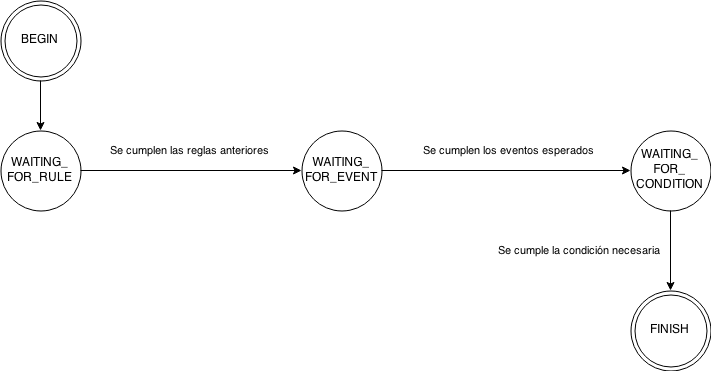
\includegraphics[width=12cm]{solucion/images/rules_flow.png}
\caption{Ciclo de vida de una regla}
\label{fig:rule_flow}
\end{figure}



Las reglas definidas dentro del procedimiento definen las acciones
que se deben llevar a cabo para completar el procedimiento, es necesario que
todas las reglas sean cumplidas para obtener un puntaje perfecto. Además definen el 
mecanismo que se utiliza para proveer una retroalimentación al usuario una vez finalizada 
la partida, pues cada regla almacena información acerca del progreso del usuario en cada paso.

%Cada regla contiene información acerca del estado del progreso del alumno en un
%paso en particular, estas reglas pueden tener como dependencias a otras reglas,
%es decir, una regla sólo se puede cumplir si una regla anterior se cumple, este
%es el caso de las reglas que definen la extracción de un torniquete, la cual
%depende de la regla que define la colocación del torniquete.  

En cuanto a la ejecución del motor de reglas, un motor de reglas \gls{eca} requiere de 
un proceso que evalúe constantemente
las reglas para verificar si las mismas deben ser lanzadas o
no\cite{bailey2004event,galton2002two}, un algoritmo comúnmente utilizado para
realizar la verificación es el algoritmo de \enquote{RETE}\cite{de2001eca}. La cantidad de
reglas definidas y la no dependencia circular entre ellas, hace innecesario la
implementación de tal algoritmo en este trabajo\cite{de2001eca}. 

De acuerdo a la descripción dada en~\ref{sec:eca}, la propuesta implementada
utiliza una ejecución inmediata, principalmente por la sencillez de las reglas,
es decir, las reglas no realizan un proceso complejo, solamente controlan el
estado del entorno y lo validan. Además, la ejecución inmediata es importante
por que el entorno no sufre modificaciones entre el evento lanzado y la
ejecución de la regla, según \cite{bailey2004event}, este es el factor más
importante para determinar el tipo de ejecución deseado.

El motor de reglas actúa sobre aquellas reglas en estado
\emph{WAITING\_FOR\_CONDITION} e invoca al procedimiento que se encarga de
validar si la regla puede ser activada (el procedimiento es único por cada
regla), si el mismo determina que la regla puede ser lanzada, el motor ejecuta
la acción de la regla y modifica el estado de la regla a \emph{FINISH}.


A continuación se muestran cada una de estas reglas definidas en la
tabla~\ref{tab:reglas_hemocultivo}, en donde se detallan cada uno de los estados
por los que pasa, a excepción de los estados BEGIN y FINISH que sólo indican el
inicio y fin de una regla. Una regla se cumple si se cumplen todas las reglas de
las cuales depende, si se lanzan los eventos esperados y si la condición del
entorno es la esperada.


\begin{table}[H]
\centering
\begin{tabulary}{\textwidth}{LLRRR}
\toprule
& Regla & Depende de las reglas & Espera a los eventos & Cuando se cumple que \\
\midrule
1  & Explicar procedimiento    &         & Explicar procedimiento    & Sea la primera regla lanzada\\
2  & Higienización de manos    & 1       & Higienización de manos    &\\
3  & Ponerse tababoca          & 2       & Ponerse tababoca          & Se realice antes de ponerse los guantes\\
4  & Ponerse gorro             & 2       & Ponerse gorro             & Se realice antes de ponerse los guantes\\
5  & Ponerse bata              & 2       & Ponerse bata              & Se realice antes de ponerse los guantes\\
6  & Calzar guantes            & 2,3,4,5 & Calzar guantes            &\\
7  & Colocar torniquete        & 10      & Colocar torniquete        & La zona correcta y mismo brazo de inserción\\
8  & Cerrar manos              & 7,10    & Cerrar puño               & Sea el mismo brazo que inserción\\
9  & Esterilizar zona          & 10      & Esterilizar zona          & Sea la misma zona que inserción\\
10 & Realizar punción          & 2       & Realizar punción          & Sea la zona correcta\\
11 & Retirar Torniquete        & 10,7    & Retirar Torniquete        & Sea el mismo torniquete que activo regla 7\\
12 & Abrir mano                & 10,8    & Abrir mano                & Sea la misma mano que activo regla 8\\
13 & Extraer Sangre            & 10,12   & Extraer Sangre            &\\
14 & Retirar Jeringa           & 10      & Retirar Jeringa           & Sea la misma jeringa que activo regla 10\\
15 & Presionar zona de punción & 10      & Presionar zona de punción & Sea la misma zona de punción\\
16 & Quitar tapaboca           & 10,3    & Quitar tapaboca           &\\
17 & Quitar gorro              & 10,4    & Quitar gorro              &\\
18 & Quitar bata               & 10,5    & Quitar bata               &\\
19 & Descalzar guantes         & 10,6    & Descalzar guantes         &\\
20 & Limpiar manos             & 19      & Limpiar manos             &\\
\bottomrule
\end{tabulary}
\caption{Reglas definidas para el procedimiento de extracción de sangre, se muestran los detalles de cada uno 
de los estados por los que pasan cada una de las reglas.}
\label{tab:reglas_hemocultivo}
\end{table}




\subsubsection{Retroalimentación y puntuación final}
\label{sec:puntuacion_hemocultivo}

Al final de una partida, la solución le brinda una retroalimentación al 
usuario como se muestra en la figura~\ref{fig:hemocultivo_retroalimentacion}.

\begin{figure}[H]
\centering 
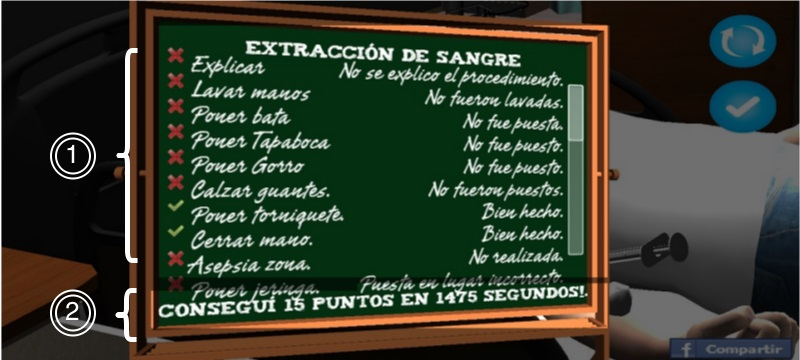
\includegraphics[width=10cm]{solucion/images/hemocultivo_retroalimentacion.jpg}
\caption{Retroalimentación y puntuación final del escenario \emph{Venopunción}.}
\label{fig:hemocultivo_retroalimentacion}
\end{figure}

En la parte $1$ de la figura~\ref{fig:hemocultivo_retroalimentacion}, se puede
ver como se brinda información al  usuario acerca de su rendimiento. Esta
información le indica los pasos que realizó de manera correcta o incorrecta y
las razones por las cuales tuvo ese desempeño.

Una regla puede quedar en uno de diferentes estados al final de la partida, cada
uno de esos estados posee un significado en el contexto del procedimiento y por
lo tanto tienen información asociada para brindar información al final de la
partida.

Cada paso en el procedimiento tiene asociado unos puntos, de acuerdo a la dificultad de realizar el
paso, estos puntos son utilizados al final de la partida para darle una puntuación al
usuario como se muestra en el punto $2$ de la
figura~\ref{fig:hemocultivo_retroalimentacion}. El puntaje final se obtiene sumando cada 
uno de los puntos logrados y calculando el porcentaje sobre el total que es de $27$. Junto al 
puntaje final se muestra el tiempo que le tomó al usuario completar el procedimiento.


\subsubsection{Registro de actividad}

Los eventos provocados por las acciones del usuario, la aplicación y el motor de 
reglas son registrados de manera transparente como se explica más adelante 
en~\ref{sec:backend_reg_eventos}. En la tabla~\ref{tab:hemocultivo_registro} se pueden observar los eventos relacionados al procedimiento.

%Existen otros tipos de eventos que no son generados por acciones, por ejemplo,
%cuando la simulación termina, el motor de reglas lanza un evento por regla,
%indicando su estado.
%
%El registro de actividades permite reproducir las \fixme{partidas}{Unificar
%    términos} y por lo tanto, es posible determinar que tareas \fixme{fueron con
%    las que los usuarios tuvieron}{pulir} un mayor número de inconvenientes.
%
%
%El registro de actividades se almacena en el dispositivo del usuario, y luego
%es enviado al \emph{backend}, esto se explica con más detalle
%en~\ref{sec:backend_reg_eventos}. 




\begin{table}[H]
\centering
\begin{tabulary}{\textwidth}{|L|L|L|}
\hline
Acción & Eventos & Motivos \\
\hline
Preparación del paciente & Explicación del procedimiento & Validación de interfaz intuitiva, 
de realización correcta de pasos y de la hipótesis \enquote{Interacción por la voz} \\
\hline
Bioseguridad inicial  & Lavado de manos, calzado de guantes, bata, tababoca y gorro & Validación 
de interfaz intuitiva, de realización correcta de los pasos y de la hipótesis 
\enquote{Bioseguridad} \\
\hline
Preparación para la extracción & Esterilización de zona, colocación de torniquete, petición de cierre de mano 
& Validación de interfaz intuitiva, de realización correcta de pasos y de validación de la hipótesis \enquote{Interacción por la voz} \\
\hline
Punción y extracción & Punzado, extracción de torniquete, petición de apertura de mano, extracción de sangre, 
extracción de jeringa & Validación de interfaz intuitiva, de realización correcta de pasos y de la 
hipótesis \enquote{Interacción por la voz} \\
\hline
Post - extracción & Presionar zona de punción & Interfaz intuitiva, realización correcta del paso \\
\hline
Bioseguridad final & Lavado de manos, descalzado de guantes, bata, tapaboca y gorro & Validación de interfaz intuitiva, de realización correcta de los pasos y de la hipótesis \enquote{Bioseguridad} \\
\hline
Utilización de redes sociales & Socialización del resultado de la partida & Medición del efecto motivador, validación de la hipótesis \enquote{Motivación}\\
\hline
\end{tabulary}
\caption{Acciones registradas durante una partida del procedimiento de venopunción, los eventos 
relacionados a ellas, y los motivos de sus registros.}
\label{tab:hemocultivo_registro}
\end{table}





\subsection{Valoración de la escala de Glasgow}

%\observacion{Más directo}
El escenario \emph{Valoración de la escala de Glasgow} se presenta en dos modos
distintos, en el primero, el usuario no conoce el estado del paciente, este modo
se conoce como \emph{Evaluar Glasgow}, y en su segundo, el usuario elige el
estado del paciente antes de iniciar la escena, este modo se conoce como
\emph{Exploración Glasgow}. 

%La reducida cantidad de diferencias entre ambos modos de la práctica permiten
%que ambas sean descritas en esta sección, las características explicadas son
%comunes para ambas, \fixme{salvo que se especifique lo contrario}{?}.

En el modo \emph{Exploración Glasgow}, antes de iniciar la escena, se le
permite al usuario seleccionar el estado del paciente mediante una interfaz 
como se puede observar en la figura~\ref{fig:glasgow_seleccion}, en
cambio, en el modo \emph{Evaluar Glasgow}, el estado del paciente no se conoce
de antemano y será responsabilidad del usuario determinarlo.

\begin{figure}[H]
\centering
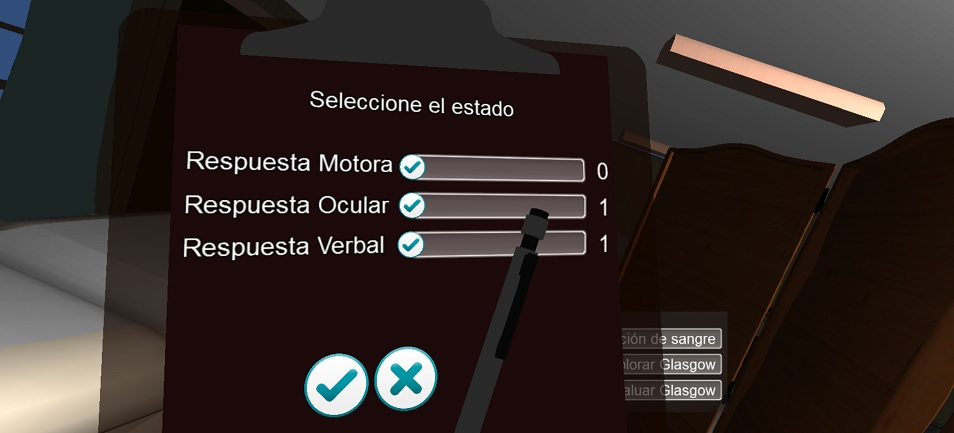
\includegraphics[width=10cm]{solucion/images/glasgow_seleccion.jpg}
\caption{Interfaz del modo \emph{Exploración Glasgow} para seleccionar el estado del 
paciente.}
\label{fig:glasgow_seleccion}
\end{figure}

%La pantalla principal de este procedimiento se muestra en la
%figura~\ref{fig:glasgow_principal}, en ella además de contar con el paciente sólo se ofrece
%una opción para finalizar la partida actual.

%\begin{figure}[H]
%\centering
%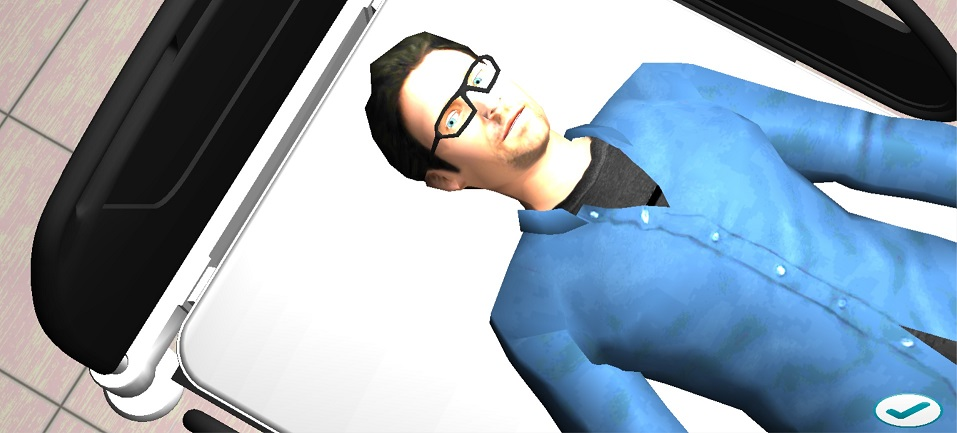
\includegraphics[width=10cm]{solucion/images/glasgow_principal.jpg}
%\caption{Pantalla principal de la escena de valoración de la escala de Glasgow.}
%\label{fig:glasgow_principal}
%\end{figure}



\subsubsection{Entidades}

%\observacion{Si la sección se llama entidades por que resalta otra cosa?}

Existen dos entidades principales, el usuario o \emph{Enfermero} y el \emph{Paciente}, 
el enfermero no almacena información, y el
paciente sólo almacena su estado, que se define al inicio. De esta forma, las
entidades no se modifican en ningún momento.

La información almacenada por la entidad paciente es su estado motor, verbal y
ocular, el cual es un conjunto de números, cuyos posibles valores se definen en
en~\ref{sec:glasgow_protocolo}, la definición de estos números varían de acuerdo
al modo de la escena como se describe a continuación:

\begin{itemize}
    \item Exploración: el usuario selecciona el estado que desea para el paciente, 
        este estado se mantendrá constante durante toda la partida.
    \item Evaluación: al inicio se crean tres números de manera
        aleatoria, el algoritmo que crea estos valores, lo hace de tal manera
        que el estado del paciente es consistente, por ejemplo, el paciente
        nunca tendrá un estado verbal \enquote{Orientado} (valor 5 en la escala)
        y un estado ocular \enquote{Ausente} (valor 1 en la escala), pues esto
        no tendría sentido, si no puede abrir los ojos (estado
        \enquote{ausente}), no puede saber donde esta (estado
        \enquote{orientado}). El estado se mantendrá constante durante toda partida.
\end{itemize}

Aunque el estado de las entidades no se modifique, esto no significa que no
puedan realizar acciones entre ellas, sino que estas acciones y los eventos
generados no alteran el estado de las entidades.


\subsubsection{Interacción con la interfaz de usuario} 

La interfaz de usuario, como se observa en la figura~\ref{fig:glasgow_principal}, es
muy sencilla, se compone de solo una opción permanente, la cual permite al
usuario finalizar la partida. Además se ve en la interfaz, al paciente, que es el 
foco principal de la cámara.
%Se observan además, las opciones que se despliegan cuando la solución detecta que
%el usuario emite palabras, conocidas como \emph{Comandos de Voz}, que permiten
%al usuario o enfermero interactuar con el paciente.

\begin{figure}[hbt]
\centering
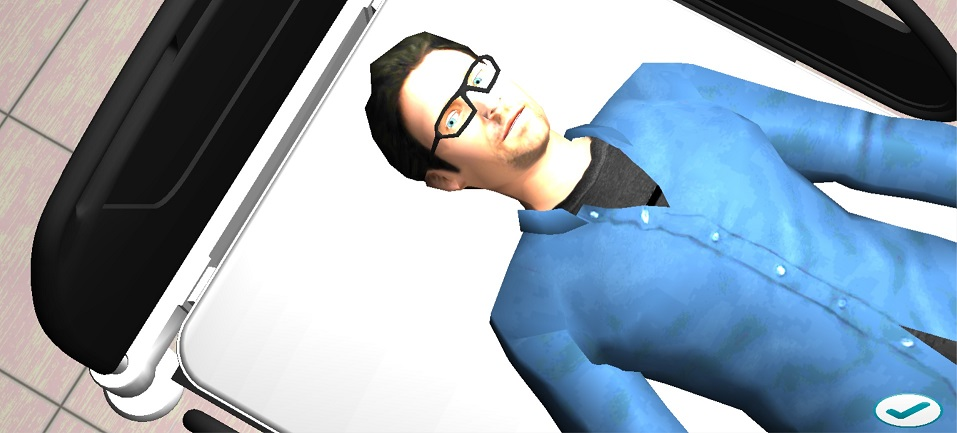
\includegraphics[width=10cm]{solucion/images/glasgow_principal.jpg}
\caption{Interfaz principal de la escena \emph{Evaluación de Glasgow}, se observa además
    la opción que permite finalizar la escena.}
\label{fig:glasgow_principal}
\end{figure}

El usuario puede interactuar con el paciente de dos modos, por un \enquote{menú
    de comandos de voz} y por opciones a través de \enquote{menú contextual}. 

\begin{itemize}

\item{\textbf{Menú Contextual}:} las opciones a través del menú contextual se
    relacionan a acciones que puede realizar el enfermero sobre una parte
    particular del cuerpo del paciente, en las extremidades, el menú despliega
    una sola opción, la cual es \emph{Pinchar} como se observa en la
    figura~\ref{fig:glasgow_menu_accion}, que provoca que el enfermero realice
    un estímulo doloroso al paciente. El paciente reacciona ante este estímulo
    dependiendo de su valoración motora y ocular. 

    \begin{itemize}
    \item Si el estado ocular del paciente es \enquote{Al dolor}, el paciente
        abrirá los ojos inmediatamente después de que se presione la opción. 
    \item  La respuesta motora varía de acuerdo a su estado, si el mismo es
        \enquote{Localiza}, el paciente mueve sus manos hasta el origen del
        dolor, si el estado es \enquote{Retira}, moverá la extremidad que
        sufrió el estímulo lejos de su posición inicial, si es
        \enquote{Flexión anormal}, el paciente reaccionará comprimiendo el
        cuerpo, indistintamente de la ubicación del estímulo doloroso, y si el
        estado es \enquote{Extiende}, el paciente extenderá el cuerpo también 
        indistintamente de la ubicación del estímulo doloroso.
    \end{itemize}

\begin{figure}[hbt]
\centering
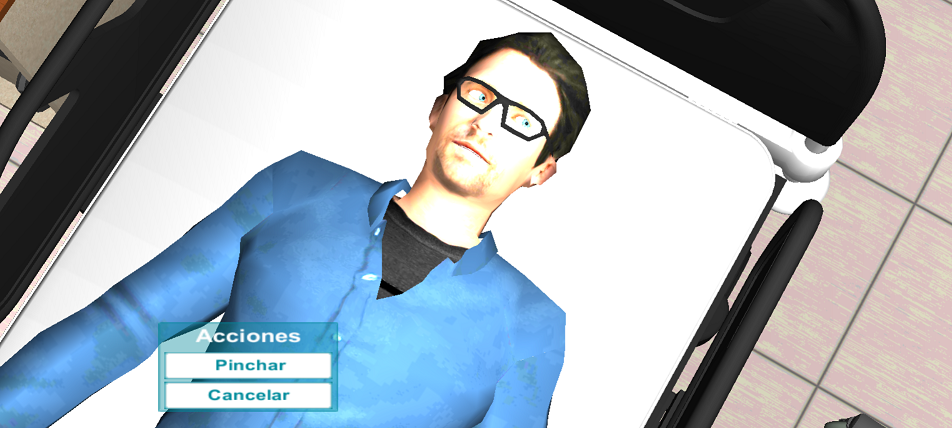
\includegraphics[scale=0.5]{solucion/images/glasgow_menu_accion.png}
\caption{Menú contextual para realizar un estímulo doloroso al paciente en el procedimiento de 
\emph{Valoración de la escala de Glasgow}.}
\label{fig:glasgow_menu_accion}
\end{figure}

\item{\textbf{Menú de comandos de voz}}

\begin{figure}[hbt]
\centering
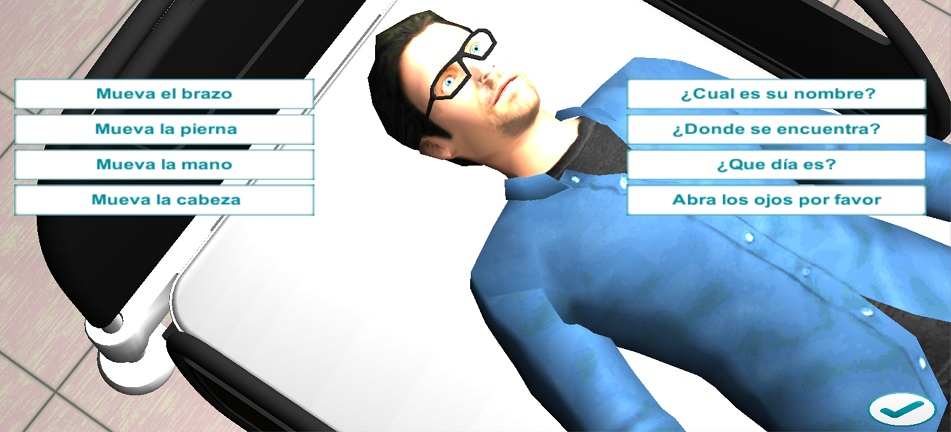
\includegraphics[scale=0.5]{solucion/images/glasgow_comandos_voz.jpg}
\caption{Interfaz de la escena \emph{Evaluación de Glasgow}, se observan los
    \emph{comandos de voz}, así como la opción que permite finalizar la escena
    (esquina inferior derecha).}
\label{fig:glasgow_gui}
\end{figure}

Las opciones del menú por comandos de voz del tipo \emph{motor}, son cuatro: 

\begin{itemize}
    \item Mueva el brazo
    \item Mueva la pierna
    \item Mueva la mano
    \item Mueva la cabeza
\end{itemize}

Estas opciones no tienen una respuesta sonora, en cambio, si el estado motor del paciente es
\enquote{Obedece}, este reacciona moviendo una extremidad, en caso
contrario, el paciente no realiza acción alguna.

Entre los comandos de voz existe una sola opción \emph{ocular}, la cual es 
\enquote{Abra sus ojos por
favor}, esta petición no tiene una respuesta sonora, y sólo si el paciente tiene un
estado ocular \enquote{Al hablar} abre los ojos, en caso contrario, no realiza
acción alguna.

Las preguntas y posibles respuestas de tipo \emph{verbal}, se pueden ver en la
tabla~\ref{tab:glasgow_opciones_respuesta}. 

\begin{table}[H]
\centering
\begin{tabulary}{\textwidth}{LCCCCC}
\toprule
\textbf{Pregunta} & \textbf{Orientado} & \textbf{Confusa} & \textbf{Palabras
    inapropiadas} & \textbf{Palabras incomprensibles} & \textbf{Ausente} \\
\midrule
¿Qué día es? & El día de la semana actual & Cualquier día de la semana menos el
correcto & La respuesta a otra pregunta en estado orientado & Gritos, gruñidos y
quejidos & No emite sonido \\
¿Cuál es su nombre? & \emph{Carlos Benitez} & Respuesta coherente sin mencionar
su nombre & Respuesta a otra pregunta en estado orientado & Gritos, gruñidos y
quejidos & No emite sonido \\
¿Donde se encuentra? & \emph{En una cama de hospital} & \emph{En mi dormitorio} &
Respuesta a otra pregunta en estado orientado & Gritos, gruñidos y quejidos & No
emite sonido \\
\bottomrule
\end{tabulary}
\caption{Posibles respuestas de acuerdo al estado verbal del paciente.}
\label{tab:glasgow_opciones_respuesta}
\end{table}

\end{itemize}

\subsubsection{Evaluación al usuario}
\label{sec:puntuacion_glasgow}

La evaluación del desempeño del usuario en la partida sólo se da en el modo \emph{Evaluación 
Glasgow}. %A continuación se describe el método de evaluación del procedimiento 
%de valoración de la escala  de Glasgow, se empieza describiendo como el 
%usuario registra su valoración en la solución.

Una vez que el usuario decida que está listo para dar un diagnóstico, procede a
finalizar la partida, en ese momento se presenta una pantalla donde el mismo
puede diagnosticar al paciente, como se observa en la
figura~\ref{fig:glasgow_gui_resultados}.

\begin{figure}[H]
\centering
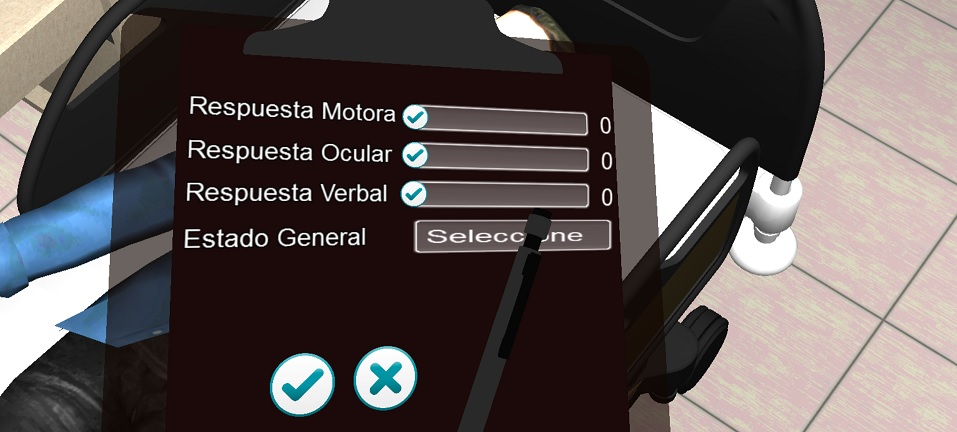
\includegraphics[width=10cm]{solucion/images/glasgow_diagnostico.jpg}
\caption{Vista de la \emph{Pantalla de diagnóstico}, donde el usuario puede
    asignar una puntuación a cada aspecto analizado del paciente.}
\label{fig:glasgow_gui_resultados}
\end{figure}

Las opciones presentadas al usuario son cuatro, puntuación verbal, ocular,
motora y un diagnóstico del estado general de conciencia del paciente. Los valores posibles 
se describen en~\ref{sec:glasgow_protocolo}.

El estado aleatorio del paciente que es generado al inicio de la partida es
guardado en una variable que no es modificada hasta que se reinicie la partida. 
Cuando el usuario confirma su diagnóstico la
aplicación lo compara con el estado guardado y de esta forma puede informar al
usuario acerca de su rendimiento en el diagnóstico. 

%\begin{itemize}
%\item{\textbf{Pantalla de diagnóstico}}
%
%Una vez que el usuario decida que está listo para dar un diagnóstico, procede a
%finalizar la partida, en ese momento se presenta una pantalla donde el mismo
%puede diagnosticar al paciente, como se observa en la
%figura~\ref{fig:glasgow_gui_resultados}.
%
%\begin{figure}[H]
%\centering
%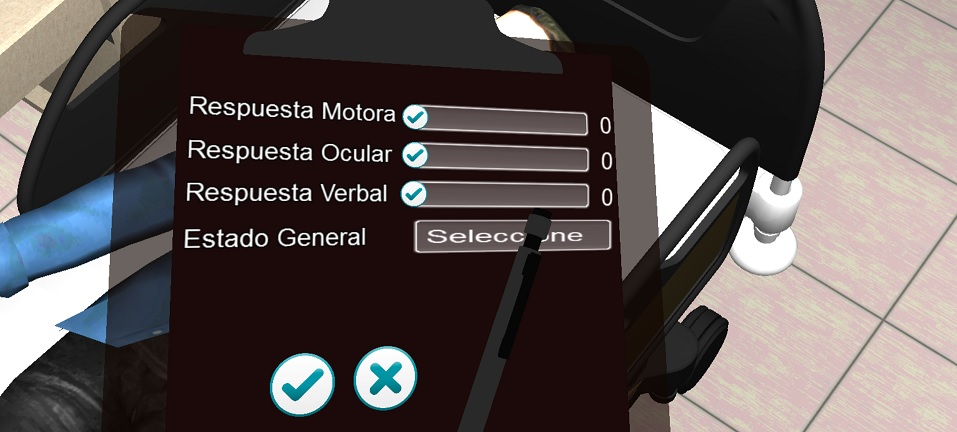
\includegraphics[width=10cm]{solucion/images/glasgow_diagnostico.jpg}
%\caption{Vista de la \emph{Pantalla de diagnóstico}, donde el usuario puede
%    asignar una puntuación a cada aspecto analizado del paciente.}
%\label{fig:glasgow_gui_resultados}
%\end{figure}
%
%Las opciones presentadas al usuario son cuatro, puntuación verbal, ocular,
%motora y un diagnóstico del estado general de conciencia del paciente. Los valores posibles 
%se describen en~\ref{sec:glasgow_protocolo}.
%
%\item{\textbf{Retroalimentación y puntuación final}}

\subsubsection{Retroalimentación y puntuación final}
%
%El estado aleatorio del paciente que es generado al inicio de la partida es
%guardado en una variable que no es modificada hasta que se reinicie la partida.
%Al final de la partida, la aplicación pide al usuario que valore el estado del
%paciente que le fue presentado, una vez que el usuario confirme su respuesta la
%aplicación la compara con el estado guardado y de esta forma puede informar al
%usuario acerca de su rendimiento en el diagnóstico. 

Cada posible respuesta dada por el usuario contiene información
relacionada al contexto del procedimiento y a la situación actual presentada, la
cual, es utilizada como retroalimentación al final de la partida como puede
verse en la figura~\ref{fig:glasgow_resultado} marcado por el número $1$. 

Para el cálculo del puntaje final que se le mostrará al usuario, por cada
respuesta dada en la pantalla de diagnóstico se asigna una puntuación de acuerdo
a que tan cerca estuvo el usuario de la respuesta correcta. Al final, se suman
estos valores y se calcula el porcentaje de acierto. El puntaje final junto a el
tiempo que tardó el usuario realizando el procedimiento se presenta como se
muestra en la figura~\ref{fig:glasgow_resultado} marcado por el número $2$.

\begin{figure}[H]
\centering
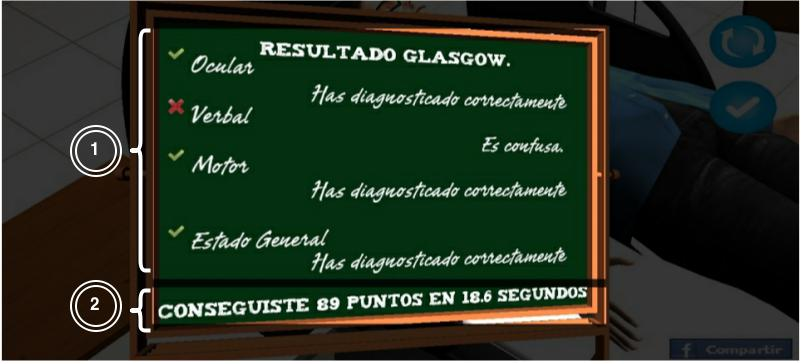
\includegraphics[width=10cm]{solucion/images/glasgow_resultado.jpg}
\caption{Retroalimentación y puntuación final del procedimiento de valoración de 
la escala de Glasgow.}
\label{fig:glasgow_resultado}
\end{figure}

%\end{itemize}

\subsubsection{Registro de actividad}
%\observacion{Todo esto es repetido}

Los eventos provocados por las acciones del usuario y por la aplicación son registrados de 
manera transparente como se explica más adelante en~\ref{sec:backend_reg_eventos}. En la 
tabla~\ref{tab:glasgow_registro} se pueden observan los eventos registrados.

%Cada acción que realiza el usuario dentro de la simulación provoca un evento, y
%estos eventos son registrados de manera transparente para el usuario. Como así
%también los eventos que genera la aplicación.
%
%El registro de actividades permite reproducir las partidas y por lo tanto, es
%posible determinar que tareas fueron con las que los usuarios tuvieron un mayor
%número de inconvenientes.



\begin{table}[H]
\centering
\begin{tabulary}{\textwidth}{|L|L|L|}
\hline
Acción & Eventos & Motivos \\
\hline
Estímulos dolorosos & Estimulación de extremidades del paciente & Validación de interfaz intuitiva \\
\hline
Acciones de voz  & Solicitudes y preguntas al paciente & Validación de la hipótesis \enquote{Interacción 
por la voz} \\
\hline
Diagnóstico del paciente & Valoración del usuario acerca de la respuesta motora, verbal y ocular 
del paciente así como su estado general & Validación de interfaz intuitiva, de realización correcta de 
la valoración \\
\hline
Utilización de redes sociales & Socialización del resultado de la partida & Medición del efecto motivador 
y validación de la hipótesis \enquote{Motivación}\\
\hline
\end{tabulary}
\caption{Acciones registradas durante una partida del procedimiento de valoración de la ecala 
de Glasgow, los eventos relacionados a ellas, y los motivos de sus registros.}
\label{tab:glasgow_registro}
\end{table}

%\observacion{Hay que depurar las cosas repetidas (esto esta abajo del primer
%párrafo de interfaz, pero me parece que incluye a las dos sub subsection)}

%\subsubsection{Interfaz de usuario}

%La interfaz de usuario, como se observa en la figura~\ref{fig:glasgow_gui}, es
%muy sencilla, se compone de solo una opción permanente, la cual permite al
%usuario finalizar la escena y mostrar la \emph{Pantalla de diagnóstico}. Se
%observan además, las opciones que se despliegan cuando la solución detecta que
%el usuario emite palabras, conocidas como \emph{Comandos de Voz}, que permiten
%al mismo interactuar con el paciente.
%
%\begin{figure}[H]
%\centering
%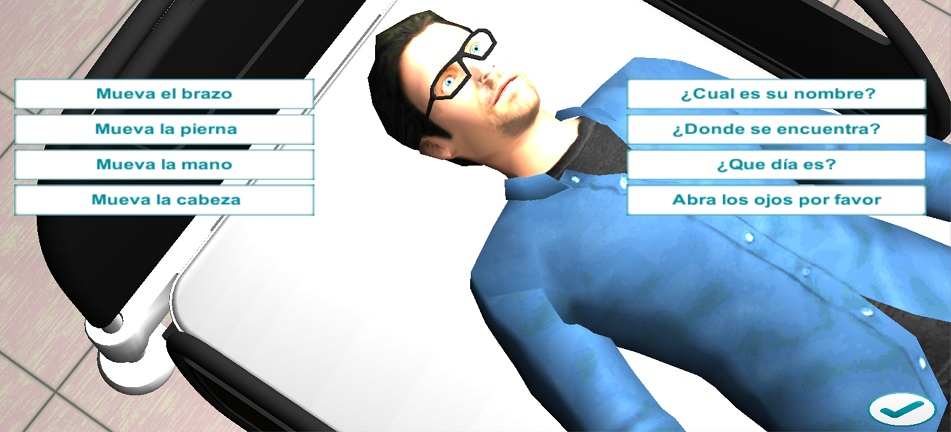
\includegraphics[scale=0.5]{solucion/images/glasgow_comandos_voz.jpg}
%\caption{Interfaz de la escena \emph{Evaluación de Glasgow}, se observan los
%    \emph{comandos de voz}, así como la opción que permite finalizar la escena
%    (esquina inferior derecha).}
%\label{fig:glasgow_gui}
%\end{figure}
%
%Además se ve en la interfaz, al paciente, que es el foco principal de la cámara.

\subsection{Pantalla de resultados}

Al finalizar tanto el escenario de \emph{Venopunción} como el escenario de \emph{Valoración de 
la escala de Glasgow}, se presenta una pantalla de resultados, la cual es
la encargada de mostrar toda la información que fue recabada durante la partida,
esta información incluye los pasos correctos e incorrectos que realizó el
usuario.

\begin{figure}[H]
\centering
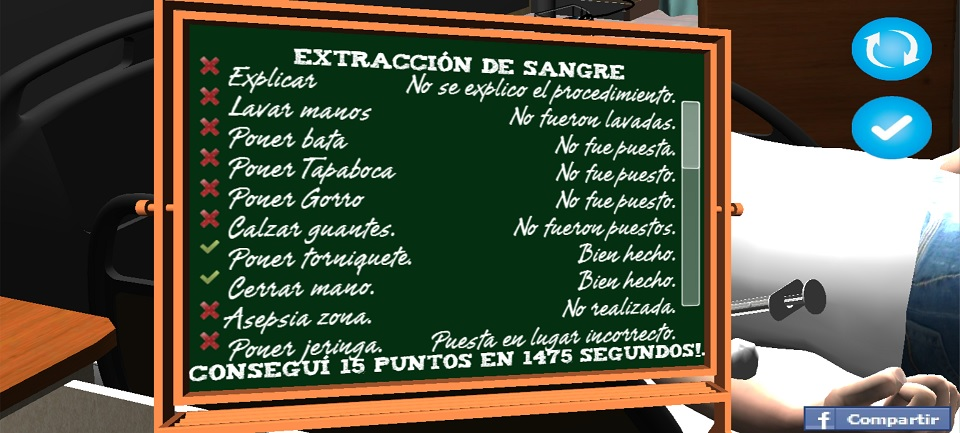
\includegraphics[scale=0.5]{solucion/images/resultado_hemocultivo.jpg}
\caption{Pantalla de resultados mostrando los pasos correctos e incorrectos, en
    la escena \emph{Glasgow}.}
\label{fig:resultados_glasgow}
\end{figure}

En la figura~\ref{fig:resultados_glasgow} se observa el diseño de la
pantalla, el título es la escena actual, un resumen de la
puntuación, y el tiempo que duró la partida.

Adicionalmente a la información de la sesión, se permite al usuario reiniciar la
partida, ir al menú de inicio, y compartir sus logros en las redes sociales.

Si el usuario presiona el botón \enquote{Facebook}, se despliega el menú de
dicha red social, permitiendo que el mismo pueda agregar un mensaje
personalizado y el resultado de la sesión se comparta con un texto similar a
\enquote{Conseguí 15 puntos en 1475 segundos, en el procedimiento de
    \emph{Venopunción} jugando con \textit{eTes\~{a}i}}.


\section{Inconvenientes de diseño}

Los mayores inconvenientes de diseño de la aplicación se dieron en el momento de
validar tanto el contenido de la aplicación como la interfaz de usuario, para
sobrellevar estos inconvenientes fueron requeridos la intervención de terceros.

A continuación se explica en detalle cada uno de los casos.

\subsection{Interfaz de usuario}

Como parte del diseño y desarrollo de la solución se realizó una prueba de
interfaz de usuario con alumnos de la carrera de Ingeniería en Informática de la
\Gls{fpuna}, estas pruebas fueron realizadas con personas que están
acostumbradas al uso de interfaces similares y que, de hecho pueden ser mas
criticas a la hora de evaluarlas. Esta prueba se explica en detalle en el
capítulo~\ref{chap:evaluacion} y los resultados en el
capítulo~\ref{chap:analisis}.

Principalmente son dos las cualidades de una interfaz gráfica que se pueden
someter a prueba: la funcionalidad y la usabilidad. Con la primera se pretende
responder preguntas como \textit{¿Se puede usar cierta función?},
\textit{¿Funciona como se espera?}, o \textit{¿Es correcta?}; y con respecto a
al usabilidad, se espera poder responder a \textit{¿Puede el usuario
    utilizar fácilmente la función?}, o \textit{¿Su uso es intuitivo y fácil de
    aprender?}\cite{fragaverificacion}.

Las pruebas de interfaces de usuario ayudan a que los usuarios puedan
concentrarse mas en el problema en vez de poner los esfuerzos en recordar todas
las opciones que ofrece la solución que se utiliza para resolver el
problema\cite{horowitz1993graphical}.

Luego de las pruebas de interfaz de usuario, se hicieron correcciones a los
problemas encontrados en la interfaz, los mayores inconvenientes fueron con
respecto a la usabilidad y la interacción tanto con el entorno como con los
objetos dentro de la simulación. Estas correcciones, como paso posterior, fueron
probadas por profesores de la carrera de enfermería del \Gls{iab} los cuales
dieron su visto bueno.

Otra de las razones por las cual la prueba fue realizada con alumnos que no
formaban parte de la población a la que iba dirigida la aplicación, es la poco
disponibilidad de tiempo con la que cuentan los alumnos de enfermería y mas aún
los profesionales que están encargados de su aprendizaje.

\subsection{Validaciones de contenido}

Llamamos validación de la simulación o la aplicación desarrollada al hecho de
que el contenido de la misma sea correcto y además que la forma de realizar o
representar dicho procedimiento este acorde al mismo. Este tipo de validaciones
fueron realizadas reiteradamente en reuniones con distintos profesores de la
carrera de enfermería del \Gls{iab}.

Cada corrección solicitada fue evaluada y aprobada posteriormente por los
mismos. Como validación final la aplicación fue presentada en totalidad frente a
un plenario de cuatro profesores del instituto.

El mayor inconveniente en cuanto a las validaciones fueron la forma de
representación tanto de la información como de la simulación de objetos.

\section{Backend de la solución}
\observacion{Podrían explicar que hacen con estos datos, no listar resultados de
    queries, pero sí explicar que tipo de información esperan obtener con esta
    concretamente. Para qué?, Por qué?, intro a análisis}

La solución almacena información detallada acerca de las acciones del usuario,
las condiciones de estas acciones y el contexto en el cual fueron ejecutadas.

Esta información es almacenada en un servidor dedicado para su posterior
análisis.

\begin{figure}[ht]
\centering
\includegraphics[scale=0.5]{solucion/images/backend_diagrama.png}
\caption{Diagrama de la interacción de los usuarios con el \textit{BackEnd}, se
    puede observar a grandes rasgos, los componentes del sistema y los servicios
    que ofrece.}
\label{fig:backend_diagrama2}
\end{figure}

En la figura~\ref{fig:backend_diagrama} se pueden observar los componentes
principales de este sistema, y su interacción con los dispositivos móviles de
los usuarios. 

\subsection{Registro de usuarios}

Para poder determinar a qué usuario corresponde qué conjunto de datos, durante la
instalación de la solución en los dispositivos móviles de los usuarios, se ingresa como
un dato adicional el número de teléfono del mismo, estos datos se registran
en el \textit{BackEnd} al mismo tiempo en el que se muestra la solución al usuario.

De esta forma, en el sistema se encuentran los datos proveídos por la
simulación, así como el nombre del usuario. Es necesario almacenar el nombre del
usuario para las diversas encuestas que se realizan (las encuestas para alumnos
que participaron en el experimento no son anónimas), de esta manera se puede
saber, dada una encuesta, a que alumno corresponde y el uso que le dio a la
solución. Estas encuestas son explicadas en detalle en~\ref{chap:evaluacion} y sus 
resultados en~\ref{chap:analisis}.

\subsection{Registro de eventos}

Las acciones que realiza el usuario son almacenadas en un archivo temporal,
dentro del dispositivo móvil del usuario, cuando este decide enviar la
información, estos datos se transmiten por la red a un servidor que almacena el
\textit{BackEnd}.

Una vez que el usuario envía sus datos de uso, el archivo de registros
local se limpia, permitiendo así que nuevos registros sean añadidos.
Adicionalmente, existe un archivo de respaldo, que contiene toda la información
que se registró del usuario, incluyendo aquellas que ya fueron enviadas al
servidor \textit{BackEnd}.

\subsection{Detalles de implementación}

El \textit{BackEnd} es un sistema web, desarrollado en \textit{Java}, y
desplegado en un servicio \textit{OpenShift}, el cual está disponible $24$ horas
al día, los $7$ días a la semana, asegurando así, que cuando el usuario desee
enviar datos lo pueda hacer sin problemas.

El sistema tiene dos servicios web que permiten el registro de usuarios y el
registro de eventos, ambos reciben una lista de elementos y los almacenan en una
base de datos \textit{PostgreSQL}.

Estos dos servicios implementan un mecanismo de seguridad sencillo, basado en usuario y
contraseña, el único objetivo de este mecanismo, es que los datos no sean
fácilmente accesibles, pues contienen datos sensibles.

La petición enviada desde la solución, contiene el número de teléfono del
usuario, un identificador único generado por \textit{Unity3D} y una lista de
eventos, en formato \Gls{json}.



% Arquitectura general
%   Flujo
%   DONDE PONER?: Motor de reglas.
%       Yo digo poner acá para que los demás sean homogéneos
%   Interacción con el entorno
% Inicio
% Extracción de sangre
%   Entidades.
%   Acciones.
%   Evaluación.
%       Reglas para la evaluación durante la ejecución.
%   Registro de actividad.
%   Interfaz de usuario.
%   Retroalimentación y puntuación final.
% Glasgow
%   Entidades
%   Acciones
%   Evaluación
%       Pantalla de diagnostico
%   Registro de actividad
%   Interfaz de usuario
%   Retroalimentación y puntuación final
% Inconvenientes de diseño
%   Interfaz de usuario
%   Validaciones de contenido
% Backend de la solución
%   Registro de usuario
%   Registro de eventos
%   Detalles de implementación
%   Utilización de información

%! TEX root = ../main.tex

\chapter{Evaluación y resultados}
\label{chap:evaluacion}


En este capítulo se detallan las metodologías utilizadas para la evaluación de la 
solución. Estas metodologías están orientadas a valorar los 
aspectos pedagógicos, de diseño, de implementación y de evaluación de la solución 
para determinar su aplicabilidad como herramienta de apoyo al proceso de 
aprendizaje.

%En este capítulo se definen las herramientas diseñadas y utilizadas para evaluar
%la utilización de los juegos serios en el aprendizaje, estas herramientas están
%orientadas a la validación de las hipótesis planteadas en la
%sección~\ref{sec:hipotesis}, así como la evaluación de aspectos pedagógicos, de
%utilidad y de la participación activa del usuario. Estas herramientas se
%utilizan para evaluar a \gls{nombre}.
%
%La evaluación se divide en cinco partes principales:

Las metodologías utilizadas son las siguientes:

\begin{itemize}

    \item \textbf{Prueba preliminar de usabilidad:} es una prueba inicial para
        medir la calidad de la interfaz y la interacción con la misma, esta
        evaluación es realizada con personas no relacionadas al área de
        enfermería, específicamente con alumnos de la carrera de
        Ingeniería en Informática de la \gls{fpuna}.

        La prueba es llevada a cabo durante el desarrollo de la solución a
        diferencia de las demás, las cuales son realizadas una vez terminada la
        solución.

    \item \textbf{Encuesta para determinar la muestra:} es una encuesta acerca del nivel de
        acceso a la tecnología que poseen los alumnos del 4to año  de la carrera 
        de licenciatura en enfermería del \Gls{iab},
        de ahora en más la población objetivo, esta encuesta sirve para definir
        la muestra.

        Se realizar la distribución de \gls{nombre} a los
        alumnos que cumplen con los requisitos mínimos y desean participar de
        las pruebas.%, luego se les realiza la siguientes pruebas para medir su
%        nivel de aceptación y aprendizaje, así como el tiempo y frecuencia de
%        utilización de la solución.

    \item \textbf{Encuesta para evaluar la solución:} es una encuesta realizada
        a cada sujeto de la muestra, donde se busca la opinión del mismo acerca
        de la solución y factores relacionados a la misma. 

    \item \textbf{Encuesta para evaluar conocimiento:} es un cuestionario que es
        completado por la población objetivo, donde se mide el conocimiento de
        los mismos. Con los resultados se busca contrastar el rendimiento de la muestra 
        con respecto a los demás alumnos.
        
        %, se utiliza a los \revisar{También participan} alumnos que
%        no forman parte de la \fixme{muestra}{}, como grupo de control.

%    \item Encuesta para evaluar el conocimiento: es un cuestionario cuyo
%        objetivo es medir el nivel de conocimiento sobre los temas simulados en
%        \gls{nombre}. 
%        
%        La muestra en esta encuesta es la población entera, los alumnos que no
%        utilizaron la aplicación forman un grupo de control.
        
    \item \textbf{Registro de actividades:} es información almacenada por la
        solución automáticamente, y contiene datos acerca del uso y el desempeño
        del alumno.
        
\end{itemize}

Además de describir las metodologías en detalle, también son mostrados y analizados 
los resultados obtenidos en cada una de las evaluaciones realizadas. Los resultados 
son expuestos en forma de tablas y gráficos para mejorar su interpretación.

%El capitulo define los objetivos de la evaluación, describe brevemente conceptos
%transversales a las técnicas utilizadas. Luego, por cada prueba realizada, se
%definen las metodologías, métricas y variables utilizadas en cada parte de la
%evaluación, y se muestran los resultados de las pruebas, al final del capítulo
%se muestran correlaciones entre las variables estudiadas.

\section{Objetivos}


\begin{itemize}
    \item Determinar el nivel de aceptación de la propuesta.
    \item 

\end{itemize}

%! TEX root = ../main.tex

\section{Métricas generales utilizadas en la evaluación}

En esta sección se describen aquellas métricas que son utilizadas por más de una
metodología para la evaluación de la solución, las cuales se consideran que son
importantes detallar.

Una de estas métricas es la escala de \textit{Likert}, la cual es una métrica
utilizada en la \emph{Encuesta para evaluar la solución} y en la encuesta
correspondiente a la \emph{Prueba preliminar de usabilidad}. Otra métrica
utilizada es la correlación de \textit{Pearson}, esta métrica es utilizada para
medir el grado de relación entre variables de las encuestas realizadas, los
registros de actividades, entre otros.

Cabe destacar que en~\cite{norman2010likert} se demuestra que, aunque el tamaño
de la muestra sea pequeña y los datos no puedan ser distribuidos normalmente o
los datos sean de escalas de tipo \textit{Likert}, los métodos paramétricos como
el análisis de varianza, la regresión y la correlación pueden ser utilizados.


\subsection{Escala de Likert}
\label{sec:likert}

Para la valoración de las variables medidas en la \emph{Prueba preliminar de
    usabilidad} y la {Encuesta para evaluar la solución} se utiliza la escala de
\textit{Likert}\cite{Allen:2007} de 7 valores posibles. La escala de
\textit{Likert} es utilizada para permitir a las personas indicar cuánto están
de acuerdo o en desacuerdo con respecto a ciertos puntos. Los valores
utilizados, son:

\begin{enumerate}
    \item Totalmente en desacuerdo.
    \item En desacuerdo.
    \item Parcialmente en desacuerdo.
    \item Neutral.
    \item Parcialmente de acuerdo.
    \item De acuerdo.
    \item Totalmente de acuerdo.
\end{enumerate}

Una vez valoradas y registradas todas las respuestas y con el objetivo de
eliminar las tendencias en la forma en la que son completadas las
encuestas\cite{Fischer2010} se utiliza el método de \emph{Doble Estandarización}
recomendado en~\cite{Pagolu2011}. Este método, consiste en dos
estandarizaciones, la primera por fila, que en este caso representa a los
individuos y la segunda por columna donde cada columna representa una de las
diferentes preguntas de la encuesta.

Siendo:
\begin{itemize}
	\item $\min_i$ la respuesta de menor valor del usuario $i$.
	\item $\max_i$ la respuesta de mayor valor del usuario $i$.
\end{itemize}

Para cada respuesta $s$ del usuario $i$, el valor ajustado, por la primera
normalización, $s_1$ se define como:

\begin{equation}
s_1{_i}=\frac{s-\min_i}{\max_i-\min_i}
\end{equation}

%\observacion{Considerar resumir}
Y luego siendo:
\begin{itemize}
	\item $groupmin_i$ la respuesta ajustada de menor valor en el grupo $i$.
	\item $groupmax_i$ la respuesta ajustada de mayor valor en el grupo $i$
\end{itemize}

Para cada respuesta ajustada $s_1{_i}$ del usuario $i$, el valor ajustado $sa_i$ se
define como:	

\begin{equation}
sa_i=\frac{s_{1_i}-groupmin_i}{groupmax_i-groupmin_i}
\end{equation}

Obteniendo así un valor normalizado, tanto por individuo, como por pregunta, en
el rango $0$ y $1$.

Para la valoración absoluta de cada  item se utiliza la media de cada columna o
respuesta a una pregunta de la encuesta.

Siendo:
\begin{itemize} 
\item $r_{k_i}$ la respuesta del usuario $i$ a la pregunta $k$.
\item $t_k$ la cantidad total de usuarios que respondieron la pregunta $k$.
\end{itemize}

El puntaje promedio de cada pregunta o item evaluado  $p_k$ en la encuesta se
define como:

\begin{equation}
p_k = \frac{\sum_{i=1}^n{r_{k_i}}}{t_k}
\end{equation}

%\subsubsection{Manejo de información faltante}
%\label{sec:informacion_faltante}
%\observacion{No repetir tanto existe}
%
%En toda encuesta pueden haber preguntas que no son respondidas por los encuestados, 
%en este tipo de situaciones existen tres posibles formas de categorizar el 
%patrón de ocurrencia de la falta de 
%respuestas\cite{leite2010performance,tsikriktsis2005review}:
%
%\begin{description}
%    \item[Información faltante completamente aleatoria:] cuando la información
%        faltante es independiente de la variable medida y de otras variables.
%    \item[Información faltante aleatoria:] cuando la información faltante depende
%        de otras variables, pero no de la variable en sí. 
%    \item[Información faltante no aleatoria:] cuando hay una relación entre la
%        información faltante y el valor de la variable.
%\end{description}
%
%Una vez categorizado el patrón de ocurrencia, existen a su vez tres
%mecanismos~\cite{tsikriktsis2005review} principales para lidiar con información
%faltante como son la eliminación, el reemplazo y los  procedimientos basados en
%modelo.~\cite{tsikriktsis2005review} recomienda utilizar un mecanismo de
%reemplazo para escalas del tipo \textit{Likert}.
%
%Las técnicas de reemplazo se clasifican en tres grandes
%grupos\cite{tsikriktsis2005review}:
%\begin{enumerate*}[label=\itshape\alph*\upshape)]
%\item basadas en el promedio,
%\item basadas en regresión, e,
%\item imputación \emph{hot deck}.
%\end{enumerate*}
%
%\fixme{De estas técnicas se seleccionó la sustitución}{Resaltar}. Basada por
%promedio ya que las relaciones entre las variables son bajas y los datos
%faltantes son menos del $10\%$. La sustitución basada por promedio se divide
%nuevamente en tres grupos\cite{tsikriktsis2005review}; promedio
%\begin{enumerate*}[label=\itshape\alph*\upshape.]
%\item total,
%\item del subgrupo, y,
%\item por caso.
%\end{enumerate*}
%
%La sustitución por promedio total es elegida debido a que la relación entre la
%variable que falta y las demás variables en los datos es relativamente baja, es
%fácil de usar y retiene la muestra. La sustitución por promedio total se realiza
%obteniendo el promedio de todas las respuestas de la pregunta cuya respuesta
%falte, la sustitución de subgrupo es similar, solo que se limita a aquellos
%sujetos del mismo subgrupo del sujeto que no respondió, y finalmente, la
%sustitución por caso, es el promedio de las respuestas válidas del sujeto.

\subsection{Correlación de variables aleatorias}
\label{sec:def_correlacion}

Las correlaciones se utilizan durante una etapa exploratoria o de observación de
la investigación para determinar las variables que tienen al menos una relación
estadística con cada uno de los diseños experimentales. Las correlaciones
también se utilizan para determinar el grado de asociación entre variables
dependientes e independientes. Por otro lado, el coeficiente de correlación se
utiliza comúnmente para cuantificar el grado de asociación entre dos variables
\cite{BoslaughStatistics2008}.

La correlación de Pearson\cite{BoslaughStatistics2008} mide la relación que
existe entre dos variables, $X$ e $Y$, el mismo esta comprendido entre $-1$ y
$1$, en su punto más bajo ($-1$) indica que una de las dos variables crece
mientras la otra decrece, y en su punto más alto ($1$), indica que ambas crecen
o decrecen conjuntamente, el valor $0$, indica que no existe una relación entre
ambas variables.

El coeficiente para las variables $X$ e $Y$ está dado por:

\begin{equation}
r = \frac{\sum_{i=1}^n{(\frac{x_i-\bar{x}}{s_x})({\frac{y_i-\bar{y}}{s_y}})}}%
{n - 1}
\end{equation}

donde:

\begin{itemize}
    \item ($x_i$, $y_i$) es el conjunto de coordenadas de las variables $X$ e $Y$.
    \item $\bar{x}$ es la media de la variable $X$.
    \item $\bar{y}$ es la media de la variable $Y$.
    \item $s_x$ es la desviación estándar de la variable $X$.
    \item $s_y$ es la desviación estándar de la variable $Y$.
    \item $n - 1$ son los grados de libertad.
\end{itemize}

%! TEX root = ../main.tex

\section{Prueba preliminar de usabilidad}
\label{sec:interfaz}

Durante el desarrollo de la solución se realizó una prueba para evaluar la 
interfaz de usuario, específicamente buscando la retroalimentación de usuarios 
acostumbrados a tecnología similar a la utilizada en la solución.

Esta prueba ayuda en el proceso de diseño e implementación de la solución con 
las características mencionadas en los objetivos del trabajo y acorde a los 
requerimientos. De esta manera se pueden identificar los aspectos que deben 
ser mejorados.

La prueba consta de dos partes importantes involucradas en la recolección
de datos para su posterior análisis. Estas partes son las siguientes:

\begin{description}

\item[Simulación:] luego de una explicación acerca de las funciones y manejos
    generales de la solución por parte de los encargados de la prueba, cada usuario
    completa una tarea que consiste en realizar el procedimiento de venopunción con la 
    solución, como ayuda, recibe una hoja con una lista de todos los pasos 
    necesarios para llevar a cabo el procedimiento.
    	
    Las simulaciones son grabadas con programas de captura de pantalla, así
    como por detectores de eventos táctiles.
    	
\item[Encuesta:] posteriormente se le provee una encuesta a cada
    usuario la cual es utilizada para obtener una idea general acerca de la
    calidad de la simulación según la percepción de los usuarios. Esta encuesta 
    contiene preguntas que son medidas mediante la escala de tipo Likert. 

\end{description} 

\subsection{Muestra}

La prueba de usabilidad de la interfaz de usuario se realiza con alumnos de la carrera de
Ingeniería en Informática de la \Gls{fpuna}, sin experiencia previa tanto con la
solución como con los procedimientos simulados, pero sí familiarizados con la
utilización de dispositivos móviles. La muestra no requiere de sujetos que sean
parte del \emph{población objetivo} ya que sólo está
orientada a mejorar aspectos de interfaz de usuario y no el contenido de la
solución, además se considera que la muestra puede brindar una evaluación más
crítica debido a su familiarización con interfaces similares a la de la
solución.

El número de muestras tomadas fue 8, ya que según~\cite{nielsen2000} son
necesarios al menos $5$ participantes para poder obtener resultados
significativos en una prueba de usabilidad. Además,~\cite{ritch2009} asegura que
la teoría de~\cite{nielsen2000} es verdadera especialmente para pruebas simples. 

Se fundamenta el número de participantes, y que es una prueba sencilla, ya que:

\begin{itemize}

\item La prueba no debería tomar más de $10$ minutos en ser realizada.

\item Se busca solamente obtener información acerca de la interfaz, y no el
    funcionamiento en sí de la simulación, pues los usuarios no son expertos en
    el área y no tienen conocimiento acerca las tareas.

\item No se busca evaluar el aspecto pedagógico de la solución sino sólo su interfaz gráfica.
%\item No se busca medir el aprendizaje del usuario en temas no relacionados a la
%    interfaz, es decir, no se mide el aprendizaje del usuario en el tema
%    simulado\revisar{No se entiende, no se mide el aspecto pedagógico solo la
%    interfaz gráfica de la simulación}.

\item El procedimiento de enfermería a realizarse con la solución está bien definido 
y los pasos necesarios están a disposición del usuario en todo momento.

\end{itemize}

\subsection{Variables}
\label{sec:evaluacion_interfaz_variables}

Antes de definir las variables, se deben primero definir los conceptos 
relacionados a los tipos de acciones que pueden realizarse sobre el paciente 
virtual en la solución, los mismos son:

%\observacion{Cual se encarga del diseño de la simulación?}
\begin{itemize}
\item \textbf{Acción por menú contextual:} se refiere a las acciones que el usuario 
    puede realizar utilizando el menú contextual que aparece sobre cada uno de los elementos 
    disponibles en la solución.
\item \textbf{Acción por menú de la \Gls{gui}:} se refiere a las 
    acciones que el usuario puede realizar seleccionando una opción en los menús 
    principales que presenta la interfaz de la solución.
\item \textbf{Acción con elemento:} se refiere a las actividades que el usuario 
    puede realizar cuando tiene seleccionado un elemento y que no involucre el 
    uso del menú contextual.
\end{itemize}


Las variables medidas durante la realización de la tarea con la solución son las
siguientes:

%\observacion{No repetir tanto la descripción en el título}

\begin{itemize}

\item \textbf{Tiempo de realización de la primera acción por tipo:} cuanto tiempo 
	le toma al usuario realizar la primera vez una acción agrupado por tipo (por menú 
	contextual, por menú de la \Gls{gui}, con elementos).

%\item \textbf{Tiempo de realización de la primera acción por menú contextual:} 
%    cuanto tiempo le toma al usuario realizar una acción por menú contextual la 
%    primera vez.
%
%\item \textbf{Tiempo de realización de la primera acción por \Gls{gui}:} cuanto 
%    tiempo le toma al usuario realizar una acción por menú de 
%    interfaz gráfica de usuario la primera vez.
%    
%\item \textbf{Tiempo de realización de la primera acción por herramienta:} cuanto 
%    tiempo le toma al usuario realizar una acción por herramienta la primera vez.

\item \textbf{Tiempo de realización de las siguientes acciones por tipo:} cuanto tiempo 
	le toma al usuario realizar las siguientes veces una acción agrupado por 
	tipo (por menú contextual, por menú de la \Gls{gui}, con elementos).
 
%\item \textbf{Tiempo de realización de las siguientes acciones por menú contextual:} 
%    cuanto tiempo le toma al usuario realizar una acción por menú 
%    contextual las siguientes veces.
%
%\item \textbf{Tiempo de realización de las siguientes acciones por \Gls{gui}:} 
%    cuanto tiempo le toma al usuario realizar una acción 
%    por interfaz gráfica de usuario las siguientes veces.
%
%\item \textbf{Tiempo de realización de las siguientes acciones por herramienta:} 
%    cuanto tiempo le toma al usuario realizar una acción por herramienta 
%    las siguientes veces.

\item \textbf{Tiempo total:} se refiere al tiempo empleado por el usuario para 
    completar la tarea asignada.

\item \textbf{Número de pasos realizados:} cantidad de pasos requeridos en la tarea 
    que son realizados por el usuario en la simulación. 

\item \textbf{Cantidad de movimientos espaciales por tipo:} número de veces en que se 
    modifica el estado de la cámara para realizar las acciones deseadas agrupados por 
    tipo (desplazamiento, acercamiento/alejamiento).

%    \observacion{Esto donde entra?}

\end{itemize}

En cuanto a la encuesta, las siguientes son las variables que fueron consideradas 
y medidas:

\begin{itemize}

\item \textbf{Calidad gráfica:} realismo y calidad de los modelos utilizados.

\item \textbf{Interacción:} desenvolvimiento en el entorno y utilización del 
    hardware.

\item \textbf{Interacción con objetos:} utilización errónea de objetos.

\item \textbf{Características del entorno:} realismo del escenario y de los 
    objetos utilizados.

\item \textbf{Usabilidad de la interfaz:} facilidad de uso de las opciones 
    proveídas por la interfaz.

\item \textbf{Integración con el hardware:} facilidad de uso de la solución con 
    un dispositivo móvil. 

\end{itemize}

\subsection{Métricas}

Para la medición de las variables relacionadas a la encuesta,  se utiliza la escala
de Likert con la \emph{Doble estandarización} explicada en la
sección~\ref{sec:likert}. 

En cambio, para la medición de las variables relacionadas a la interacción del usuario con 
la solución se utilizan las grabaciones registradas durante las pruebas y las
las siguientes métricas:

%Para el análisis de la encuesta realizada a los usuarios, se utiliza la escala
%de Likert con la \emph{Doble estandarización} explicada en la
%sección~\ref{sec:likert}, y en el análisis de la interacción del usuario con la
%solución se utilizan las grabaciones registradas durante la prueba.
%
%Haciendo uso de las variables descriptas anteriormente, las métricas
%utilizadas son las siguientes:

\begin{itemize}
    
\item \textbf{Tiempo promedio de realización de las siguientes acciones por menú contextual:} 
    se obtiene dividiendo la cantidad total de tiempo empleado en realizar acciones por menú 
    contextual por el número de veces que se realizaron esas acciones, sin considerar la primera 
    vez. 
    
\item \textbf{Tiempo promedio de realización de las siguientes acciones por \Gls{gui}:} 
    se obtiene dividiendo la cantidad total de tiempo empleado en realizar acciones por \Gls{gui} 
    por el número de veces que se realizaron esas acciones, sin considerar la primera 
    vez. 
    
\item \textbf{Tiempo promedio de realización de las siguientes acciones por herramienta:} 
    se obtiene dividiendo la cantidad total de tiempo empleado en realizar acciones por 
    herramienta por el número de veces que se realizaron esas acciones, sin considerar la 
    primera vez. 
    
\item \textbf{Promedio de pasos correctos:} se obtiene dividiendo la cantidad de 
    pasos requeridos realizados por los usuarios sobre la cantidad de pasos requeridos. 
    
\item \textbf{Promedio de movimientos por tipo:} se obtiene dividiendo el número de 
    movimientos que fueron realizados agrupados por tipo (desplazamiento, acercamiento/
    desplazamiento) por la cantidad de usuarios.
    
\item \textbf{Promedio del tiempo total:} se obtiene dividiendo el tiempo total empleado 
    por los usuarios para completar la tarea asignada por el número de usuarios.

\end{itemize}

\subsection{Resultados obtenidos}
\label{sec:res_interfaz}

A continuación de muestran y analizan los resultados obtenidos en la prueba. Los resultados 
se dividen en \emph{simulación} y \emph{encuesta} para una mejor comprensión.

\subsubsection{Simulación}

Las grabaciones realizadas a las sesiones de los usuarios se utilizan para medir
el grado de facilidad de aprendizaje de la interfaz de usuario.

Dados los tres tipos de acciones descritos en~\ref{sec:evaluacion_interfaz_variables}, la
tabla~\ref{tab:interfaz_tiempo_acciones} muestra el tiempo, en segundos,
que le tomo a cada usuario realizar una acción la primera vez y 
el tiempo que les tomo en promedio las demás veces, para cada uno de los tipos 
de acciones.

%\observacion{Hacer énfasis en la comparación entre el primer y los siguientes}

\begin{table}[!hbt]
\centering
\begin{tabular}{|c|c|c|c|c|c|c|}
\hline
\rowcolor{gris} \textbf{} & \multicolumn{2}{|c|}{\textbf{Menú Contextual}} &
\multicolumn{2}{|c|}{\textbf{Menú de la Interfaz}} &
\multicolumn{2}{|c|}{\textbf{Herramienta}}\\
\hline
\rowcolor{gris} Usuario & Primera & Siguientes & Primera & Siguientes & Primera & Siguientes \\
\hline 1 &  8 &  2.25 &  3 & 9.14 & 11 & 3.0 \\
\hline 2 & 30 &  7.00 &  4 & 3.57 &  7 & 4.5 \\
\hline 3 &  5 &  2.25 &  5 & 1.86 &  1 & 1.0 \\
\hline 4 &  2 & 13.00 &  4 & 2.00 &  1 & 0.5 \\
\hline 5 & 18 &  2.75 &  6 & 4.43 &  6 & 3.0 \\
\hline 6 &  4 & 14.25 & 11 & 7.86 & 13 & 4.0 \\
\hline 7 &  5 &  8.00 &  4 & 4.71 & 20 & 2.5 \\
\hline 8 &  3 &  2.33 & 10 & 3.57 &  3 & 6.5 \\
\hline
\textbf{Promedio} & 9.38 & 6.37 & 5.88 & 4.64 & 7.75 & 3.125 \\
\end{tabular}
\caption{Tiempo por acciones la primera vez y las siguientes veces que se realizo}
\label{tab:interfaz_tiempo_acciones}
\end{table}

En la tabla~\ref{tab:interfaz_tiempo_acciones} se observa consistentemente una 
mejora en el tiempo de realización de un tipo de acción con respecto a la primera vez 
que es realizada. 

En la figura~\ref{fig:interfaz_tiempo_acciones} se observa como en promedio el
usuario aprende, y en las siguientes acciones similares demora menos tiempo,
este es un factor importante y es el objetivo de esta prueba pues muestra que la
interfaz es fácil de usar, y con tres tipos de acciones, el usuario puede
utilizarla sin mayores inconvenientes. Se observa una mejoría del $30\%$ en las
\emph{Acciones por menú contextual}, $21\%$ en las \emph{Acciones por menú de la
    \Gls{gui}} y finalmente, una mejoría del $60\%$ en las \emph{Acciones con elementos}.

%\begin{figure}[H]
%\centering
%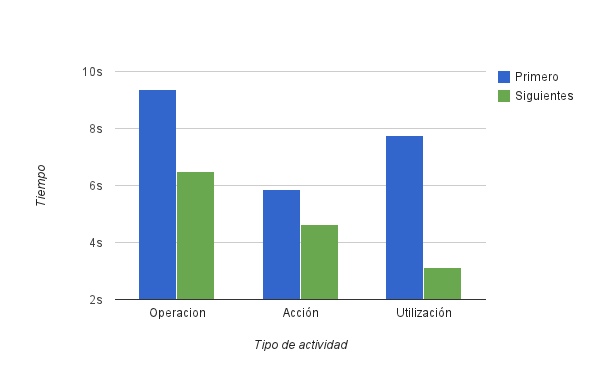
\includegraphics[width=14cm]{resultados/imagenes/interfaz_tiempo_actividades.png}
%\caption{Tiempo por tipo de actividad}
%\label{fig:interfaz_tiempo_acciones}
%\end{figure}

\begin{filecontents}{interfazuso.dat}
n   p       s
1	9.38	6.48
2   5.88	4.64
3   7.75	3.13
\end{filecontents}
\pgfplotstableread{interfazuso.dat}{\InterfazUso}

\begin{figure}[H]
    
        \centering
        \begin{tikzpicture}[scale=1]
           \begin{axis}[ybar,%
              legend pos=outer north east,
              xmin=1,
              xmax=3,
              x=2.5cm,
              enlarge x limits={abs=1cm},
              xtick=data,
              symbolic x coords={0,1,2,3,4},
              ymin=0,ymax=10,
              %ytick={0,2,4,6,8,10},
              xticklabels={Contextual,Interfaz,Herramienta},
              ylabel= Tiempo (s),
              xlabel= Tipo de acción,
              bar width=10pt,
              %enlarge x limits={abs=2},
                ]   
        \addplot[color=blue,ybar,fill=blue!75,area legend] table [x = {n}, y = {p}] {\InterfazUso};
        \addlegendentry{Primer}
        \addplot[color=red,ybar,fill=red!75,area legend] table [x = {n}, y = {s}]
        {\InterfazUso};
        \addlegendentry[align=left]{Promedio \\ siguientes}
        \end{axis}
        \end{tikzpicture}
        \caption{Tiempo por tipo de acción}
        \label{fig:interfaz_tiempo_acciones}
\end{figure}

En la tabla~\ref{tab:interfaz_cantidad_espaciales} se observa la cantidad de
movimientos espaciales realizados por los usuarios, se observa que en promedio
se desplazaron $10,88$ veces por el escenario, y $6,75$ veces acercaron o
alejaron la cámara del paciente.

%\observacion{Hay que dejar bien en claro de donde sale esto, por que es
%importante entender el significado de esta diferencia}

\begin{table}[H]
\centering
\begin{tabular}{lrrr}
\toprule
\textbf{Jugador}  & \textbf{Desplazamiento} & \textbf{Acercamiento/alejamiento} & \textbf{Total} \\
\midrule
1        & 18         & 2    & 20 \\
2        & 7          & 8    & 15 \\
3        & 14         & 12   & 26 \\
4        & 9          & 14   & 23 \\
5        & 5          & 8    & 13 \\
6        & 14         & 4    & 18 \\
7        & 16         & 3    & 19 \\
8        & 4          & 3    &  7 \\
\midrule
\textbf{Promedio} & \textbf{10,88}      & \textbf{6,75} & \textbf{17,63} \\
\bottomrule
\end{tabular}
\caption{Cantidad de movimientos espaciales}
\label{tab:interfaz_cantidad_espaciales}
\end{table}

No existe una cantidad mínima o máxima de movimientos que el usuario debe realizar para acercar, 
alejar o desplazar la cámara. Los datos mostrados en la tabla~\ref{tab:interfaz_cantidad_espaciales} 
muestran que no son necesarias demasiados movimientos. Teniendo en cuenta esta información y la 
proveída en la tabla~\ref{tab:interfaz_tiempo_total}, se concluye 
que en promedio los usuarios realizan $1,7$ movimientos por minuto.

\begin{table}[!hbt]
\centering
\begin{tabular}{lrrr}
\toprule
\textbf{Alumno} & \textbf{Tiempo (min)} \\
\midrule
1        & 8:32 \\
2        & 6:03 \\
3        & 8:33 \\
4        & 5:17 \\
5        & 6:55 \\
6        & 8:40 \\
7        & 7:03 \\
8        & 10:27 \\
\midrule
\textbf{Promedio} & \textbf{7:41} \\
\bottomrule
\end{tabular}
\caption{Tiempo de prueba por usuario}
\label{tab:interfaz_tiempo_total}
\end{table}

El tiempo total que se observa en la tabla~\ref{tab:interfaz_tiempo_total},
muestra que en promedio a cada alumno le tomo $7:41$ minutos realizar todos los
pasos especificados, es importante notar que este tiempo incluye el tiempo de
adaptación. 

La tabla~\ref{tab:interfaz_acciones} nos muestra la cantidad de pasos
realizados por los alumnos de un total de 19. Se observa que en promedio 
realizaron $16.75$ pasos.
%esto permite identificar en que parte del procedimiento los usuarios tienen
%inconvenientes en cuanto al uso de la interfaz.

\begin{table}[H]
\centering
\begin{tabular}{lrrr}
\toprule
\textbf{Alumno} & \textbf{Pasos realizados (19)} \\
\midrule
1 & 19 \\
2 & 15 \\
3 & 18 \\
4 & 15 \\
5 & 18 \\
6 & 16 \\
7 & 19 \\
8 & 14 \\
\midrule
\textbf{Promedio} & \textbf{16,75} \\
\bottomrule
\end{tabular}
\caption{Pasos realizados por alumno}
\label{tab:interfaz_acciones}
\end{table}



\subsubsection{Encuesta}


La encuesta es utilizada para obtener el grado de
disconformidad de los usuarios con respecto a la solución. Se utiliza la disconformidad 
para resaltar los puntos débiles, así, aquellas variables que tengan el mayor porcentaje serán
las que deban ser mejoradas.

%Las preguntas que forman parte de la  encuesta son agrupadas en cuanto a
%aspectos de calidad gráfica, interacción con el entorno, interacción con los
%objetos, características del entorno, usabilidad de la interfaz e integración
%con el hardware.

En la tabla~\ref{tab:interfaz_disconformidad_metrica} se observan que las mayores 
disconformidades son la usabilidad de la interfaz de usuario que llega al $51\%$, la 
interacción de los usuarios con el entorno que llega al $50\%$ y la interacción con los 
objetos que llega al $49\%$. Otras disconformidades con menor porcentaje son las
características del entorno con un  $33\%$, la integración con el hardware con
un $27\%$ y por último la calidad gráfica con un $17\%$.

%\observacion{Hay que explicar que estas pruebas se hicieron de forma previa a
%las demás y que se arreglan algunos casos}

\begin{table}[H]
\centering
\begin{tabular}{lr}
\toprule
Variable & Disconformidad (0-1)\\
\midrule
Calidad Gráfica         & 0.17 \\
Interacción Entorno     & 0.50\\
Interacción Objetos     & 0.49\\
Características Entorno & 0.33\\
Usabililidad Interfaz   & 0.51\\
Integración Hardware    & 0.27\\
\bottomrule
\end{tabular}
\caption{Disconformidad por variable}
\label{tab:interfaz_disconformidad_metrica}
\end{table}

%La conclusión de esta prueba de interfaz, es que si bien, pudo ser utilizada sin
%mayores inconvenientes, existe un alto grado de disconformidad con la interfaz,
%además cabe resaltar, los sujetos de prueba son personas acostumbradas al uso de
%tecnologías similares. Otros puntos débiles encontrados en esta prueba son la
%interacción con el entorno y  con los objetos.

Como consecuencia de los resultados obtenidos, la usabilidad de interfaz y la interacción con objetos y 
con el entorno son mejoradas para obtener la versión final de la solución que es utilizada por 
los estudiantes de enfermería. Las demás pruebas mencionadas en este capítulo son realizadas con 
la versión final de la solución.
%elementos sufren modificaciones a fin de su utilización con usuarios no
%técnicos.

%Las demás pruebas mencionadas en este capítulo son realizadas con la versión
%final de la solución, la cual es obtenida luego de las mejoras realizadas a los
%puntos débiles detectados por esta prueba.

%! TEX root = ../main.tex

\section{Encuesta de ubicación}
\label{sec:ubicacion}

Para recabar información acerca del nivel de acceso  de los alumnos a la
tecnología, se realiza una encuesta que cuenta con diez preguntas, las cuales
buscan conocer el modelo de dispositivo móvil, el acceso a
Internet, y la predisposición de cada alumno a ayudar en la prueba.

Con los resultados de la encuesta de ubicación tecnológica, se seleccionan
aquellos alumnos que poseen dispositivos móviles que superan o igualan las
especificaciones descritas más adelante. De esta encuesta se obtendrán los 
usuarios que formarán parte de la población que evaluará la versión final de 
la solución.

\subsection{Muestra}

En el año $2014$, el \Gls{iab} cuenta con $124$ alumnos en el cuarto año  de la 
carrera de Licenciatura en Enfermería distribuidos en
tres secciones, estos alumnos son considerados la población objetivo. De los 124, 93 de
ellos estuvieron interesados en completar la encuesta.

\subsection{Variables}

Se definen $3$ factores necesarios para que un alumno pueda ser considerado como
sujeto de prueba, el primero es la predisposición del mismo a participar de la
prueba, el segundo es que posea un dispositivo móvil que supere los requisitos
mínimos explicados más adelante y el tercero es que tenga algún tipo de conexión a 
internet desde el dispositivo móvil pues 
los registros de actividad de cada dispositivo deben ser enviados y almacenados 
para su posterior interpretación y análisis. A continuación se describen las variables 
consideradas.


\begin{itemize}

\item \textbf{Requisitos mínimos:} son aquellos requerimientos técnicos con los que 
    debe cumplir completamente el dispositivo móvil del usuario para que la 
    solución tenga un desempeño que garantice una experiencia fluida a la hora de 
    utilizarla. Estos requisitos son:
    \begin{itemize}
        %%\item Sistema Operativo Android $4.0$ o superior
        \item Memoria ram de $512$MB o superior.
        \item Velocidad de procesador de $800$ GHz o superior.
        \item \Gls{gpu} OpenGL ES 2.0 o superior.
        %\item Conexión frecuente a internet.
    \end{itemize}
    Los requisitos de \textit{hardware} mencionados, son requeridos por las
    características de la simulación, una \Gls{gpu} es requerida por los gráficos en 
    tres dimensiones.

\item \textbf{Tipo de acceso a internet:} el tipo de acceso a internet que posee el 
    usuario en su dispositivo móvil. Puede ser una de las siguientes opciones:
    plan post-pago, paquetes pre-pago, acceso ocasional y sin acceso.
    
\item \textbf{Sistema Operativo:} se refiere al tipo de sistema operativo que posee 
    el dispositivo móvil del usuario.

%    \observacion{Donde se menciona?}
    
\end{itemize}

\subsection{Métricas}

Las métricas utilizadas para estudiar los datos recogidos son sencillas ya que
sólo buscan determinar la población que evaluará la solución, estas métricas son
las siguientes:

\begin{itemize}
\item Porcentaje de encuestados con dispositivos móviles que cumplen y que no cumplen con 
los requisitos mínimos.
\item Porcentaje del tipo de acceso a internet de los encuestados desde sus dispositivos móviles.
\item Porcentaje del tipo de sistema operativo que poseen los dispositivos móviles de los 
encuestados.
\end{itemize}


\subsection{Resultados obtenidos}


%Como se indicó en la sección~\ref{sec:ubicacion}, se agrupa a los
%\fixme{alumnos}{De donde?} encuestados de acuerdo a las características de sus
%dispositivos móviles y del acceso a internet.

%El acceso a internet es un requisito importante, pues para que los mismos puedan
%enviar su progreso y así se registre la utilización de la solución, así, es
%necesario que los usuarios tengan un acceso ocasional a internet. 

En la figura~\ref{fig:ubicacion_acceso_internet} se puede observar que de 93 alumnos 
encuestados, el $94,6\%$ tiene acceso a internet al menos en algún momento y que
solo el $5.4\%$ no tiene acceso a internet en sus dispositivos móviles. Considerando 
sólo estos datos, el $94,6\%$ de los alumnos podría utilizar la solución.

%esto
%permite que tengan acceso a la solución el $94,6\%$ de los alumnos.

%\begin{figure}[H]
%\centering
%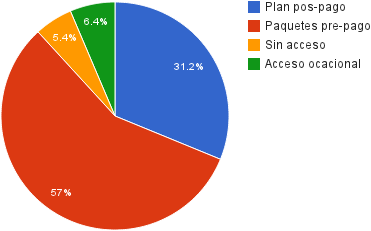
\includegraphics[scale=0.5]{resultados/imagenes/ubicacion_acceso_internet.png}
%\caption{Acceso a internet desde dispositivos móviles}
%\label{fig:ubicacion_acceso_internet}
%\end{figure}

 \begin{figure}[H]
        \centering
        \begin{tikzpicture}[thick,scale=0.7, every node/.style={transform shape}]
            \pie[
                %explode=.2,
                text=legend,
                %style=drop shadow,
                %radius=3,
                %scale font,
                explode={0.1,0.1,0.3,0.3}
                ]%
            {%
                31.2 / Plan pos-pago,
                57   / Paquetes pre-pago,
                5.4  / Sin acceso,
                6.4  / Acceso ocasional}
        \end{tikzpicture}
        \caption{Acceso a internet desde dispositivos móviles}
        \label{fig:ubicacion_acceso_internet}
\end{figure}

%La utilización en dispositivos móviles es un requisito necesario para
%\fixme{la}{Utilizar la solución} solución

Los dispositivos móviles son un requisito para utilizar la solución, 
en la figura\ref{fig:ubicacion_sistemas_operativos} se muestran los sistemas operativos
móviles utilizados por los alumnos encuestados, si bien el motor de videojuego 
utilizado permite generar clientes a diversos sistemas operativos, es importante conocer el sistema
operativo que poseen los alumnos para realizar pruebas.

En la figura~\ref{fig:ubicacion_sistemas_operativos} se puede observar que
\emph{Android} lidera con un $61.3\%$, le sigue Windows Phone con un $12.9\%$.
Si bien, según la tabla~\ref{tab:comparacion_motores_juegos}, \emph{Unity3D}
soporta la mayoría de los sistemas operativos, aún es importante hacer pruebas
sobre un sistema operativo específico. Se selecciona \emph{Android} por ser el
sistema operativo con mayor cuota entre los alumnos.

%\begin{figure}[H]
%\centering
%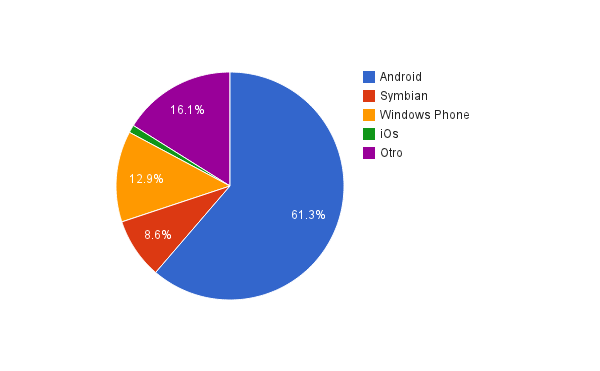
\includegraphics[scale=0.5]{resultados/imagenes/ubicacion_sistemas_operativos.png}
%\caption{Sistemas operativos móviles utilizados}
%\label{fig:ubicacion_sistemas_operativos}
%\end{figure}

 \begin{figure}[H]
        \centering
        \begin{tikzpicture}[thick,scale=0.7, every node/.style={transform shape}]
            \pie[
                text=legend,
                rotate=61.3,
                explode={.1,.2,.2,.2}
                ]%
            {%
            61.3 / Android,
             8.6 / Symbian,
            12.9 / Windows Phone,
            17.2 / Otros}
        \end{tikzpicture}
        \caption{Sistemas operativos móviles utilizados}
	    \label{fig:ubicacion_sistemas_operativos}
\end{figure}
    

Por último, se divide a los encuestados para determinar cuantos de ellos
tiene dispositivos móviles que cumplen los requisitos mínimos para utilizar la
solución propuesta según lo descrito en la sección~\ref{sec:ubicacion}. En la
figura~\ref{fig:ubicacion_requisitos_minimos} se puede observar que el $18,3\%$
de los encuestados cumplen con los requisitos.

Si bien los requisitos de la solución no son elevados para los estándares
actuales, la figura~\ref{fig:ubicacion_requisitos_minimos} nos muestra que el
$18.3\%$ tiene dispositivos de alta gama, el cual es un porcentaje mayor al
esperado. Se observa además que cerca del
$90\%$ posee un dispositivo de gama media o superior, la penetración de los
dispositivos móviles es muy alta en los estudiantes de enfermería del \Gls{iab}.

%\begin{figure}[H]
%\centering
%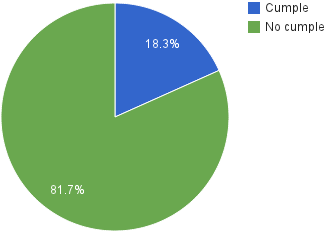
\includegraphics[scale=0.5]{resultados/imagenes/ubicacion_requisitos_minimos.png}
%\caption{Dispositivos que cumplen con los requisitos mínimos para la prueba}
%\label{fig:ubicacion_requisitos_minimos}
%\end{figure}

\begin{figure}[H]
       \centering
       \begin{tikzpicture}[thick,scale=0.7, every node/.style={transform shape}]
           \pie[
                text=legend,
                explode=.1
                ]%
            {%
                81.7 /  No Cumple,
                18.3 /  Cumple
            }
        \end{tikzpicture}
        \caption{Dispositivos que cumplen con los requisitos mínimos para la prueba}
		\label{fig:ubicacion_requisitos_minimos}
\end{figure}

Considerando los datos mostrados, el $17$ alumnos cumplen con los requisitos para utilizar y evaluar 
la solución.




\section{Registro de actividades}
\label{sec:registro}

El registro de actividades ayuda a identificar las  fortalezas y debilidades de
la solución en cuanto al diseño y utilidad. Para que los alumnos puedan formar
una opinión válida acerca de la solución primero deben experimentar con la
misma, para ello se instala la solución en los dispositivos móviles de los
alumnos.

La instalación de la solución se lleva a cabo en el \Gls{iab}, se procede a
mostrar un vídeo de la simulación, explicar la interfaz de usuario y realizar
una muestra de como desenvolverse en el entorno. El período de prueba se
extiende por 20 días, el mismo no es asistido, es decir, existen factores que no
pueden ser controlados, como:

\begin{itemize}
    \item Tiempo dedicado a la simulación por parte del alumno.
    \item Que todas las acciones provengan del alumno.
    \item Que sólo el conocimiento del alumno es puesto a prueba, es decir, no
        se puede controlar que no reciba ayuda externa.
\end{itemize}

Por estos motivos, el uso de la solución propuesta no puede ser considerado el
único factor relacionado con los resultados obtenidos en la \emph{Encuesta para
    medir el conocimiento}, cuyos resultados son mostrados más adelante en la
sección~\ref{sec:objetiva}.

La solución propuesta almacena información relacionada a la actividad del
usuario, incluyendo cuándo y cómo realiza las acciones, los pasos que realiza,
el orden y las condiciones de la escena cuando realiza cada acción.

El registro como un todo es enviado cada vez que el usuario desee, este envío
requiere una conexión a internet, por ello no es automático. Adicionalmente el
último día de la prueba, todos los registros fueron enviados para que sean
analizados.

\subsection{Muestra}

La muestra está conformada por los $11$ alumnos que aceptaron formar parte de 
la prueba y poseen dispositivos móviles que cumplen con los requisitos
mínimos descritos en la sección~\ref{sec:ubicacion}.

La utilización de $11$ alumnos es suficiente, ya que según estudios presentados
en~\cite{nielsen2000}, mientras menos experiencia tengan los sujetos de estudio
con la solución planteada, serán necesarios menos para detectar un gran
porcentaje de errores y fortalezas, y según~\cite{ritch2009}, una base de $10$ a
$12$ es suficiente para obtener resultados estadísticamente válidos.

\subsection{Variables}

%La utilización de la solución, y el registro de las actividades genera una
%gran cantidad de información, los factores que se desean medir están
%relacionados a aquellos que pueden ser contrastados con los resultados de la
%encuesta objetiva.

Los registros de actividades nos permiten obtener información relevante acerca
de cómo se utilizó la solución y cuál fue el desempeño de los usuarios, las variables a medir son 
las siguientes:


\begin{description}

\item[Cantidad de partidas:] se define como el número de veces que un usuario
    inicia una escena. 

\item[Tiempo total:] es la suma del tiempo empleado en todas las partidas.

\item[Tiempo total de partidas por usuario y por tipo:] es el tiempo total 
    empleado para jugar las partidas discriminadas por tipo y por usuario.

\item[Cantidad de acciones:] es la cantidad total de acciones realizadas por 
    los usuarios.
 
\item[Cantidad de partidas realizadas por usuario y por tipo:] es el número de 
    partidas jugadas por usuario discriminado por el procedimiento al que 
    corresponde.

\item[Cantidad de usuarios:] es el número de usuarios que utilizaron la solución.
    
\item[Puntuación de las partidas:] dado el registro de reglas cumplidas en una partida 
    del procedimiento de venopunción o el diagnóstico dado por el usuario 
    en una partida del procedimiento de valoración de la escala de Glasgow, se 
    puede obtener el desempeño del usuario en las partida. 
%    Esto puede ser contrastado 
%    con la puntuación obtenida por el usuario en la \emph{Encuesta Objetiva}.

%\item[Puntuación por regla cumplida] Las variables definidas
%    en~\ref{sec:objetiva}, pueden ser contrastadas con la puntuación obtenida
%    por los alumnos en la simulación.

\end{description}

\subsection{Métricas}

Las métricas utilizadas para el análisis de los registros de actividades son las siguientes:

\begin{description}
\item[Promedio de tiempo por partida:] se obtiene dividiendo el tiempo total empleado 
    en las partidas por el número de partidas.
\item[Promedio de acciones por partida:] se obtiene dividiendo la cantidad total de 
    acciones realizas por los usuarios por el número de partidas.
\item[Promedio de partidas por usuario:] se obtiene dividiendo el número total de partidas
    por el número de usuarios que utilizaron la solución.
\item[Total de sesiones jugadas por tipo:] es la suma del número de partidas jugadas por los 
    usuarios discriminadas por tipo.
\item[Total de tiempo jugado por tipo:] es la suma de la cantidad de tiempo empleado en una 
    partida por los usuarios discriminado por tipo.
\item[Promedio de siguientes puntajes por tipo y por usuario:] se obtiene dividiendo la suma 
    de los puntajes obtenidos en cada tipo de escenario por la cantidad de veces que jugó el 
    usuario, a excepción de la primera vez.
\end{description}

%Además de las métricas descritas también se utiliza la correlación de Pearson como se 
%explica en \ref{sec:correlacion} para identificar las relaciones entre los datos obtenidos en 
%la \emph{Encuesta Objetiva} y los obtenidos en el \emph{Registro de actividades}.

\subsection{Resultados obtenidos}

%Las actividades de los usuarios son registradas y almacenadas para su análisis, a
%continuación se presentan los resultados de ese análisis, el mismo fue descrito
%en~\ref{sec:registro}, 

En la tabla~\ref{tab:log_total} se observa un resumen del experimento, en cuanto a tiempo, partidas y acciones.


\begin{table}[H]
\centering
\begin{tabular}{lrrrrrrrr}
%\toprule
%\textbf{Variable}                         & \textbf{Valor} \\
\toprule
Partidas                         & 99 \\
Primera partida					 & 4 de noviembre de 2014 \\
Última partida					 & 23 de noviembre de 2014 \\
\midrule
Tiempo total                     & 11134 s \\
Promedio de tiempo por partida   & 112 s \\
\midrule
Acciones                         & 2944 \\
Promedio de acciones por partida & 30 \\
\midrule
Usuarios                         & 8 \\
Promedio de partidas por usuario & 12 \\
\bottomrule
\end{tabular}
\caption{Resumen de la información extraída del registro de actividades}
\label{tab:log_total}
\end{table}

La cantidad de partidas jugadas por usuario en el procedimiento de venopunción, se muestra en la
tabla~\ref{tab:log_hemocultivo_partida}, se observa que existen $3$ alumnos que no
participaron de la prueba o no se registraron sus actividades.

\begin{table}[H]
\centering
\begin{tabular}{lrrrrrrrr}
\toprule
& \multicolumn{2}{c}{Venopunción} \\
\cmidrule(lr){2-3} 
Alumno   & Sesiones jugadas & Tiempo jugado (s) \\
\midrule
 1       & 5                & 1202 \\
 2       & 19               & 2507 \\
 4       & 5                & 398  \\
 5       & 6                & 768  \\
 6       & 17               & 2371 \\
 7       & 7                & 707  \\
 9       & 1                & 126  \\
10       & 8                & 960  \\
\midrule
Total   & 68               & 9039 \\
\bottomrule
\end{tabular}
\caption{Número de partidas y tiempo total por alumno en segundos, en la escena
    de venopunción.}
\label{tab:log_hemocultivo_partida}
\end{table}



Los registros pueden no ser registrados sí
\begin{enumerate*}[label=\itshape\alph*\upshape)]
    \item el usuario utilizó la solución, no envió los datos y, luego
        desinstaló la solución o borró los datos de la misma, o,
    \item el usuario no utilizó la solución.
\end{enumerate*}

En la tabla~\ref{tab:log_glasgow_random_partida}, se observa la cantidad de
sesiones y tiempo total por alumno, en la escena de \textit{Glasgow}, en modo de
evaluación. Se observa que $5$ alumnos participaron en $22$ sesiones, en total
jugaron $1768$ segundos. En cambio, en la tabla~\ref{tab:log_glasgow_custom_partida} se 
observa que $4$ alumnos participaron en $9$ sesiones y en total jugaron $327$ segundos. 
Los alumnos prefirieron jugar en el modo que les permitía diagnosticar al paciente.

\begin{table}[H]
\centering
\begin{tabular}{lrrrrrrrr}
\toprule
& \multicolumn{2}{c}{Glasgow (Evaluación)} \\
                   \cmidrule(lr){2-3} 
Número de alumno   & Sesiones jugadas                            & Tiempo jugado (s) \\
\midrule
1     & 4  & 211 \\
2     & 8  & 738 \\
4     & 3  & 132 \\
6     & 1  & 97  \\
7     & 6  & 590 \\
\midrule
Total & 22 & 1768 \\
\bottomrule
\end{tabular}
\caption{Número de partidas y tiempo total por alumno en segundos, en la escena
    \textit{Glasgow}, en modo evaluación}
\label{tab:log_glasgow_random_partida}
\end{table}


\begin{table}[H]
\centering
\begin{tabular}{lrrrrrrrr}
\toprule
& \multicolumn{2}{c}{Glasgow (Exploración)} \\
                   \cmidrule(lr){2-3} 
Número de alumno   & Sesiones jugadas                            & Tiempo jugado (s) \\
\midrule
1        & 2 & 79 \\
2        & 3 & 80 \\
4        & 3 & 89 \\
6        & 1 & 79 \\
\midrule
Total   & 9 & 327 \\
\bottomrule
\end{tabular}
\caption{Número de partidas y tiempo total por alumno en segundos, en la escena
    \textit{Glasgow}, en modo exploración}
\label{tab:log_glasgow_custom_partida}
\end{table}


En las tablas~\ref{tab:log_hemocultivo_puntaje}
y~\ref{tab:log_glasgow_random_puntaje} se muestran los primeros puntajes y un
promedio de los puntajes siguientes obtenidos por cada alumno en los
procedimientos de venopunción y de la evaluación de la escala de
Glasgow. Se debe tener en cuenta el tiempo y la cantidad de veces que cada
alumno jugó cada uno de los procedimientos para valorar los resultados
mostrados. 

\begin{table}[H]
\centering
\begin{tabular}{lrrrrrrrr}
\toprule
& \multicolumn{2}{c}{Venopunción} \\
\cmidrule(lr){2-3} 
Número de alumno  & Primer Puntaje & Siguientes Puntajes \\
\midrule
 1                & 11             & 14.3 \\
 2                & 9              & 10.6 \\
 4                & 3              & 3.3  \\
 5                & 3              & 6.8  \\
 6                & 3              & 5.8  \\
 7                & 4              & 4    \\
 9                & 16             & \\
10                & 3              & 7.2  \\
\midrule
\textbf{Promedio} & 6.5            & 7.42 \\
\bottomrule
\end{tabular}
\caption{Puntaje obtenido la primera vez y el promedio de los puntajes de las siguientes veces
    por alumno, en la escena de venopunción}
\label{tab:log_hemocultivo_puntaje}
\end{table}


\begin{table}[H]
\centering
\begin{tabular}{lrrrrrrrr}
\toprule
& \multicolumn{2}{c}{Glasgow (Evaluación)} \\
                   \cmidrule(lr){2-3} 
Número de alumno   & Primer Puntaje & Siguientes Puntajes \\
\midrule
1     & 1 & 1.5 \\
2     & 2 & 2.3 \\
4     & 1 & 1.5 \\
6     & 2 & 2 \\
7     & 0 & 1 \\
\midrule
\textbf{Promedio} & 1.2 & 1.66 \\
\bottomrule
\end{tabular}
\caption{Puntaje obtenido la primera vez y el promedio de los puntajes de las siguientes veces
    por alumno, en la escena \textit{Glasgow}, en modo evaluación}
\label{tab:log_glasgow_random_puntaje}
\end{table}

En las tablas~\ref{tab:log_hemocultivo_puntaje}
y~\ref{tab:log_glasgow_random_puntaje} se observa que los alumnos que participaron de la prueba
mejoran su desempeño a medida que aumenta el número de partidas. 

%Es importante notar que la cantidad de partidas no es uniforme entre los
%alumnos, es decir hay alumnos con más de $10$ partidas y alumnos con menos de
%$5$, por ello, no es posible demostrar que existe un progreso a medida que
%aumenta el número de partidas.

Por último, en la figura~\ref{fig:utilizacion_hora} se puede observar la distribución de 
las partidas por hora del día. Los picos de uso de la solución se dan a las $13:00$ horas, 
horario de almuerzo, a las $17:00$ horas, fin de las actividades académicas y a las $01:00$ horas, 
horario libre. De esta manera los datos muestran que el mayor uso de la solución se da en los 
horarios libres de los alumnos, es decir, los alumnos deciden usar la solución en su tiempo libre.

\begin{filecontents}{utilizaciontiempo.dat}
Hora	Cantidad
 0	 0
 1	 9
 2	 4
 3	 2
 4	 0
 5	11
 6	 8
 7	 3
 8	 5
 9	 7
10	 7
11	12
12	15
13	 9
14	 6
15	 0
16	 0
17	 0
18	 0
19	 0
20	 0
21	 0
22	 0
23	 1
24	 0
\end{filecontents}
\pgfplotstableread{utilizaciontiempo.dat}{\UtilizacionTiempo}

\begin{figure}[H]
	\centering
    \begin{tikzpicture}[thick, scale=1.2]
        \begin{axis}[
            title={},
            xlabel={Hora},
            ylabel={Partidas},
            xmin=0, xmax=24,
            ymin=0, ymax=16,
            xtick       = {0  , 3  , 6  , 9  , 12 , 15 , 18 , 21 , 24},
            xticklabels = {12 , 15 , 18 , 21 ,  0 , 3  ,  6 ,  9 , 12},
            %ytick={0,.25,.50,.75,1},
            legend pos=north east,
            ymajorgrids=true,
            xmajorgrids=true,
            grid style=dashed,
        ]
         
        \addplot[color=blue,fill=blue!5] table [x = {Hora}, y = {Cantidad}] {\UtilizacionTiempo};
        \end{axis}
    \end{tikzpicture}
    \caption{Utilización de la solución por hora del día}
    \label{fig:utilizacion_hora}
\end{figure}

%! TEX root = ../main.tex
\section{Encuesta Subjetiva}

En el análisis de los resultados, existieron alumnos que no respondieron todas
las preguntas, para tratar este tipo de casos, es importante analizar la
naturaleza del patrón de datos faltantes\cite{carpita2011imputation}. Existen
tres posibles formas de categorizar el patrón de ocurrencia de falta de
respuestas\cite{leite2010performance}\cite{leite2010performance}\cite{tsikriktsis2005review}:


\begin{description}
    \item[Información faltante completamente aleatoria] Cuando la información
        faltante es independiente de la variable medida y de otras variables.
    \item[Información faltante aleatoria] Cuando la información faltante depende
        de otras variables, pero no de la variable en sí. 
    \item[Información faltante no aleatoria] Cuando hay una relación entre la
        información faltante y el valor de la variable.
\end{description}

Los datos muestran que la información faltante es completamente aleatoria en
relación a la variable medida y a las demás variables, de hecho, una sola
encuesta tiene información faltante, así, se establece que el tipo de
información faltante es \emph{Información faltante completamente aleatoria}.

Existen tres mecanismos\cite{tsikriktsis2005review} principales para lidiar con
información faltante, eliminación, reemplazo, y procedimientos basados en modelo
(?Model-based procedure XXX).\cite{tsikriktsis2005review} recomienda utilizar
un mecanismo de reemplazo para escalas del tipo Likert.

Las técnicas de reemplazo se clasifican en tres grandes
grupos\cite{tsikriktsis2005review}:
\begin{enumerate*}[label=\itshape\alph*\upshape.]
\item basadas en la promedio,
\item basadas en regresión, y,
\item imputación \emph{hot deck}.
\end{enumerate*}

La sustitución basada por promedio, se divide nuevamente en tres grupos;
promedio
\begin{enumerate*}[label=\itshape\alph*\upshape.]
\item total,
\item del subgrupo, y,
\item por caso.
\end{enumerate*}
La sustitución del promedio total se realiza obteniendo el promedio de todas las
respuestas de esta pregunta, la sustitución de subgrupo es similar, solo que se
limita a aquellos sujetos del mismo subgrupo del sujeto que no respondió, y
finalmente, la sustitución por caso, es el promedio de las respuestas válidas
del sujeto.

En su resumen de las diferentes técnicas y cuando se deben utilizar cada una,
\cite{tsikriktsis2005review}, recomienda la utilización de la sustitución basada
en promedio por caso. 

De esta forma se reemplazan los valores faltantes en la encuesta, con el
promedio del sujeto.

%! TEX root = ../main.tex

\section{Encuesta para evaluar el conocimiento}
\label{sec:objetiva}

A fin de obtener información acerca del conocimiento de los alumnos  que forman parte de la 
población objetivo, es decir, aquellos que utilizaron 
la solución propuesta y los que no la utilizaron, los cuales constituyen el grupo 
de control, se realiza una encuesta que consta de diez preguntas.

La encuesta mide el nivel de conocimiento del alumno sobre los dos temas
simulados, contiene preguntas de nivel básico, medio y avanzado. Las mismas son
formuladas utilizando la lista de competencias básicas que debe tener un alumno
para aprobar la materia \textbf{Enfermería en Urgencias II}. Las preguntas son
verificadas  por los profesores de la cátedra. Cada pregunta tiene el mismo
peso, así la puntuación más baja obtenible es $0$, y la más alta es $10$.

De esta manera se busca evaluar la influencia pedagógica de la 
solución como herramienta de apoyo al aprendizaje.


\subsection{Muestra}
%\observacion{Se repite mucho lo de las muestras hay 2 universos nomas?}

La población objetivo cuenta con $124$ alumnos, de los cuales $11$ son la muestra seleccionada
para la prueba de la solución, y los $113$ alumnos restantes son utilizados
como grupo de control.

\subsection{Variables}

Se busca medir el puntaje total de los alumnos en la \emph{Encuesta para evaluar el conocimiento}. Esto 
se obtiene de la siguiente manera.

Siendo:

\begin{itemize}
    \item $po_i{_k}$ la respuesta del usuario $i$ a la pregunta $k$
    \item $n$ total de preguntas, igual a 10
    \item $tc$ total de alumnos en el grupo de control, igual a 113.
    \item $t$ total de alumnos, igual a 124
    \item $ts$ total de sujetos de estudio, igual a 11.
\end{itemize}

Se define el puntaje total $pto_i$ del alumno $i$ como, 

\begin{equation*}
    pto_i = \sum_{j=1}^n{po_i{_j}}
\end{equation*}


\subsection{Métricas}

Como se mencionó, la \emph{Encuesta para evaluar el conocimiento} busca medir el rendimiento de los 
alumnos, para ello se utiliza como métrica principal el promedio de acierto, 
tanto del conjunto total de alumnos de la población objetivo, como de los que participaron de la
prueba, y del grupo de control por separado.

Se define el promedio total de los alumnos, $promtotal$ como:

\begin{equation*}
    promtotal = \frac{\sum_{i=1}^t{pto_i}}{t}
\end{equation*}

Se obtienen los promedios del grupo de control ($promcontrol$) y del grupo de alumno que
participo en la prueba para evaluar la solución ($promsujetos$) de la misma manera.

\subsection{Resultados obtenidos}
\label{sec:res_objetiva}

Como se detalló en la sección~\ref{sec:objetiva}, la encuesta realizada a cada
usuario, parte de la prueba, es utilizada para obtener una comparación en cuanto
al rendimiento de los usuarios que forman parte de la muestra y los que forman
parte del grupo de control.


%\observacion{A esta altura ya no se entiende que es promcontrol}
%\observacion{No estaría mal poner algún tipo de información que diga a que
%aspectos se relacionad cada pregunta}

La tabla~\ref{tab:objetiva_rendimiento_por_pregunta} muestra el nivel de acierto
en promedio por pregunta de los usuarios que forman parte de la muestra y de los
que forman parte del grupo de contro. Según estos datos, en el $60\%$ de los casos 
hay una leve mejoría en cuanto al nivel de acierto para los usuarios que forman 
parte de la muestra.

\begin{table}[H]
\centering
\begin{tabular}{lrrr}
\toprule
& \multicolumn{3}{c}{Promedio} \\
\cmidrule(lr){2-4}
\textbf{Pregunta} & 
\textbf{Muestra} & 
\textbf{Grupo Control} & 
\textbf{Total} \\ 
\midrule
ES1. Torniquete           & 0.36 & 0.18 & 0.20 \\
ES2. Guantes              & 0.64 & 0.60 & 0.60 \\
ES3. Manos                & 0.09 & 0.14 & 0.13 \\
ES4. Bioseguridad         & 0.27 & 0.25 & 0.26 \\
ES5. Explicación          & 0.82 & 0.56 & 0.59 \\
\midrule
EG1. Diagnóstico Global 1 & 0.00 & 0.18 & 0.16 \\
EG2. Diagnóstico Global 2 & 0.64 & 0.51 & 0.53 \\
EG3. Respuesta ocular     & 0.45 & 0.28 & 0.29 \\
EG4. Respuesta motora     & 0.18 & 0.32 & 0.31 \\
EG5. Respuesta verbal     & 0.36 & 0.45 & 0.45 \\
\midrule
\textbf{Sumatoria}: & 3.82 & 3.47 & 3.49  \\
\bottomrule
\end{tabular}
\caption{Rendimiento promedio de usuarios por pregunta}
\label{tab:objetiva_rendimiento_por_pregunta}
\end{table}

Los datos sólo sugieren levemente una tendencia a la mejoría de los puntajes
para los usuarios que forman parte de la muestra, sin embargo, estos datos no
pueden ser tomados para realizar conclusiones ya que la cantidad de sesiones de
juego por usuario no se considera suficiente para que el uso de la solución
propuesta afecte realmente en el aprendizaje del usuario. Cabe destacar, que 
tanto la muestra como el grupo de control respondieron a la encuesta luego del examen 
final de la materia \emph{Enfermería en Urgencias II}, la cual requería el dominio de ambos 
temas simulados.

\section{Correlación entre variables}
\label{sec:correlacion}

En la tabla~\ref{tab:all_correlation} se observa la correlación entre cinco
variables estudiadas, a fin de observar si existe alguna correlación entre los
valores, se utiliza la correlación de \emph{Pearson}, descrita
en~\ref{sec:correlacion}.

\begin{table}[H]
\centering
\begin{tabular}{lrrrrrr}
\toprule
        &
\begin{sideways}\textbf{Tiempo de Uso}\end{sideways}             &
\begin{sideways}\textbf{Encuesta solución}\end{sideways}        &
\begin{sideways}\textbf{Encuesta conocimiento}\end{sideways}         &
\begin{sideways}\textbf{Puntaje Máximo Extracción}\end{sideways} &
\begin{sideways}\textbf{Puntaje Máximo Glasgow}\end{sideways}    \\
\midrule
Tiempo de Uso             & 1    & -0.2  & 0.15  & 0.62 & 0.41 & 0.78 \\
Encuesta solución         & -0.2 & 1     & -0.07 & 0.04 & 0.11 & -0.28\\
Encuesta conocimiento     & 0.15 & -0.07 & 1     & 0.44 & 0.44 & 0.02 \\
Puntaje máximo Extracción & 0.62 & 0.04  & 0.44  & 1    & 0.96 & 0.44 \\
Puntaje máximo Glasgow    & 0.41 & 0.11  & 0.44  & 0.96 & 1    & 0.27 \\
\bottomrule               & 0.78 & -0.28 & 0.02  & 0.44 & 0.27 & 1    \\
\end{tabular}
\caption{Correlación entre factores estudiados} 
\label{tab:all_correlation}
\end{table}

Las correlaciones fuertes, que se observan en la
tabla~\ref{tab:all_correlation}, son:

\begin{itemize}
    \item Tiempo de uso y puntaje máximo extracción, $0,62$, correlación
        positiva fuerte.
    \item Tiempo de uso y puntaje máximo Glasgow, $0,78$, correlación positiva
        muy fuerte.
    \item Puntaje máximo extracción y encuesta objetiva, $0,44$, correlación
        positiva fuerte.
\end{itemize}


La tabla~\ref{tab:all_correlation} indica que existe una correlación positiva
fuerte ($0,62$ y $0,78$) entre el tiempo de uso y el puntaje más alto obtenido,
\fixme{lo que sugiere que mientras más se utiliza la solución, se obtienen mejores
resultados}{Guardaaaa correlación no es igual que casualidad}. 

Una correlación positiva fuerte entre el puntaje máximo obtenido en la
Extracción y la encuesta objetiva ($0,44$), sugiere que existe una relación entre
el nivel de conocimientos de los alumnos y su desempeño en la práctica.


%\chapter{Conclusión}
\label{chap:conclusion}

\observacion{\begin{itemize}
    \item Agrupar por temas
    \item Agregar referencias hacia atrás
    \item Evitar mapear términos
    \item Mapear objetivos específicos con la conclusión.
\end{itemize}}
\observacion{Poner por partes la conclusión}

% INTRO
Durante este trabajo \fixme{de grado}{estudio el ... y} se desarrolló una
aplicación para dispositivos móviles con el fin de que sirva de apoyo en el
proceso de aprendizaje de los estudiantes de la carrera de enfermería,
utilizando a los juegos serios y el construccionismo como base.

% ACCESIBILIDAD
\fixme{
    La mayoría de los estudiantes cuenta con al menos un dispositivo móvil con el
    cual tienen acceso a internet por lo que la idea de darle ubicuidad nos resulto
    factible, no sólo por que contaban con este medio sino por que ello significaba
    brindarles la oportunidad de utilizar la herramienta en cualquier lugar y
    momento. La mayoría de los estudiantes que formaron parte de la prueba
    concluyó que el uso de la solución les parecía útil para complementar el estudio
    en clase o laboratorio y que ayuda a comprender los procedimientos.
}{que quieren decir?}

% VENTAJAS
Los estudiantes mencionan como ventajas de la solución, el poder realizar
prácticas de procedimientos de manera más confiada ya que el paciente con el que
se interactúa es sólo virtual, la oportunidad de poder practicar en todo momento
y además, también mencionaron que el uso de la solución los acercaba más a la
tecnología.

Los profesores encargados del proceso de aprendizaje de los estudiantes de
enfermería con los que trabajamos en el desarrollo de este trabajo en todo
momento estuvieron abiertos al uso de las \Gls{tic} en forma de juegos serios,
incluso mencionaron la idea de poder utilizarlos en clase. Esto nos lleva a
pensar en que están abiertas las posibilidades de inclusión de la tecnología en
formas mas innovadoras con respecto a la forma de utilización en la actualidad
en nuestro país.

\fixme{Los juegos serios no sólo permiten al estudiante experimentar, poner a
    prueba y adquirir conocimientos sino que, debido a sus características
    lúdicas, ayuda en la motivación siendo además una opción diferente con
    respecto a las demás opciones tecnológicas utilizadas en el ámbito
    educativo. }{Mencionar datos de la prueba}

% DESARROLLO

% CARACTERISTICAS
En cuanto al diseño de juego serio con las características de la solución, es
importante la retroalimentación que pueda tenerse de parte de los profesores,
así como es importante también la retroalimentación de los estudiantes ya que
son estos últimos los que utilizan la herramienta. Es importante mantener una
buena relación con los profesores, y además se debe mantener el interés de estos
en el proyecto, pues es necesario obtener la mayor cantidad de conocimientos y
detalles que puedan brindar en cuanto al contenido de la aplicación y, sobre
todo, para que evalúen cada paso realizado en la solución.

% COMUNICACIÓN CON PROFESIONALES
Debido a la apretada agenda que poseen los profesionales de salud, poder
reunirse con ellos frecuentemente y en un largo periodo de tiempo para validar
ideas y contenido de la aplicación resulta ser muy difícil, por lo cual es
importante recabar la máxima cantidad de información posible.

% INTERACCIÓN
En cuanto a la interacción con la solución implementada, siempre es preferible
que sea lo más natural posible, la forma de uso de la aplicación no debería ser
un obstáculo para utilizarla, la forma en que los elementos son representados y
utilizados dentro de la aplicación debe ser realista, o en todo caso debe
representar de la mejor manera la realidad de acuerdo a las limitaciones.

% ENCUESTA
En cuanto a las pruebas de la aplicación, es importante elaborarlas con la
opinión profesional de los expertos, sus validaciones son indispensables, ya que
ellos son especialistas en el contenido. Los estudiantes que formarán parte de
la prueba deben estar bien informados sobre el objetivo de la solución y la
validez de la misma, ya que deben estar interesados en probarla y ayudar para
facilitar la evaluación. 

% LOGS
Es importante registrar la actividad de los usuarios, sobre todo con
herramientas que ofrecen ubicuidad y son probadas a distancia. Además de las
pruebas, se deben diseñar encuestas que puedan obtener información que no se
puedan apreciar con las pruebas y registros de actividades, sobre todo la
apreciación final de los estudiantes de la solución como una herramienta útil
para el aprendizaje.


% PUEDE IR CONCLUSION SOBRE EL USO DE LA HERRAMIENTA ESPECIFICAMENTE EN EL AREA DE ENFERMERIA
La utilización de motores gráficos modernos facilita la creación de juegos
serios, relacionados a procedimientos del área de enfermería, permiten crear y
manipular entornos realistas sin demasiadas complicaciones. En cuanto a las
limitaciones, tanto tecnológicas como de utilización, presentadas por los
dispositivos móviles dificultan la interacción con el entorno, la interacción a
través de dispositivos móviles debe ser cuidadosamente diseñada para proveer de
una interacción fluida. 

% ESTO DEFINITIVAMENTE DEBE IR AL FINAL
Como conclusión final, consideramos interesante la investigación de herramientas
como la solución propuesta en este trabajo ya que la tendencia actual es que las
tecnologías tengan un papel más activo en el proceso de enseñanza-aprendizaje, y
las nuevas pedagogías requieren que sea así. Como se reflejan en varios
artículos, los estudiantes del nuevo milenio están acostumbrados a las nuevas
tecnologías y tienen otros estilos de aprendizaje, por lo que debe asumirse el
desafío de incorporar a la tecnología con mayor fuerza, aportando aún más
dinamismo en los procesos de enseñanza-aprendizaje. Creemos además, que el
factor motivacional que puede brindar este tipo de herramientas influirá
positivamente en los estudiantes y en el profesores.

% APRECIACIÓN PERSONAL

\observacion{\begin{itemize}
\item Agrupar las conclusiones por categoría
\item Referenciar secciones cuando se afirma algo respecto a los
    resultados
\item Enumerar o bullets
\end{itemize}}

% Puntos de los que se podria dar una conclusion


% - La mayoria de los estudiantes cuenta con un dispositivo movil desde el cual tienen acceso a internet
% - La mayoria de los estudiantes opino que el uso de herramientas como la solucion es util para complementar 
% el estudio en clase o laboratorio.
% - La mayoria de los estudiantes opino que la solucion es una herramienta que ayuda a memorizar y comprender 
% los procedimientos
% - La mayoria considero sumamente importante que las herramientas le proporcionen una retroalimentacion sobre 
% su rendimiento pero desean mucha informacion acerca de los errores cometidos, no solo breves justificaciones.
% - La mayoria considero que la herramienta provee facilidades para el estudio
% - En preguntas abiertas los estudiantes dieron como ventaja de la solucion el poder realizar practicas de 
% procedimientos de manera mas confiada ya que el paciente es ficticio, la oportunidad de poder practicar 
% en todo momento, mencionaron tambien que los acerca mas a la tecnologia
% - En el diseño y desarrollo de herramientas de este tipo es importante la retroalimentacion que tengamos de 
% parte de los maestros encargados del aprendizaje pero tambien de los alumnos ya son ellos los que la mayoria
% de las veces las utilizaran.
% - Los profesores del area estuvieron abiertos al uso de las TIC presentados de esta forma, incluso 
% mencionaron poder utilizarlos en clase.
% - Los juegos serios no solo permiten al estudiante experimentar, poner a prueba y adquirir conocimientos sino que
% debido a las caracteristicas ludicas que posee ayuda en la motivacion de los mismos, siendo ademas una opcion 
% diferente e innovadora con respecto a las demas
% - En cuanto al diseño, es preferible que la interaccion con la aplicacion sea lo mas natural posible.
% - En cuanto al diseño, es preferible que la forma de uso de los elementos dentro de la aplicacion sean lo 
% mas real posible o en todo caso represente de la mejor manera la realidad de acuerdo a las limitaciones.
% - En el diseño y desarrollo, es importante mantener una buena relacion con los profesionales encargados de 
% la formacion de los estudiantes ya que se debe obtener la mayor cantidad de conocimientos y detalles de los 
% mismos, y ademas debe matenerse el interes de estos profesionales para que evaluen cada paso tomado en 
% la realizacion de la solucion
% - Debido a la apretada agenda que poseen los profesionales de salud poner reunirse con ellos todo el tiempo y 
% un largo periodo resulta muy dificil, por lo cual es importante ir preparados a estas reuniones y ser los
% mas breves y concisos posible.
% - En cuanto a las pruebas, es importante elaborarlas con la opinion profesional de los maestros, su validacion es 
% muy importante ya que ellos son los especialistas en el contenido en la que la herramienta esta basada.
% - En cuanto a las pruebas, es importante que los estudiantes esten informados del objetivo de la herramienta, 
% de la validez de la misma, ya que deben estar interesados en probarla y ayudar en su evaluacion para que 
% pueda ser valorada de manera correcta.
% - En cuanto a las pruebas, es importante tener un registro de actividad de los usuarios, sobre todo con 
% herramientas que ofrecen ubicuidad y son probados a distancia dada esta caracteristica importante, de 
% otra manera seria imposible evaluar su uso.
% - En cuanto a las pruebas, es importante diseñar encuestas que puedan obtener informacion que no puedan ser 
% apreciadas solo con el uso de registro de actividad de usuarios, es importante la apreciacion final de los 
% estudiantes sobre todo en cuanto a lo que implica la solucion como una herramienta util
% - Actualmente existen motores de juegos completos que ofrecen grandes facilidades para el desarrollo de videojuegos.
% - Se considera interesante la investigacion de herramientas como la solucion ya que la tendencia actual es que 
% las tecnologias tengan un papel mas activo en el aprendizaje, y las nuevas pedagogias requiren que sea asi. 
% Los estudiantes del nuevo milenio estan acostumbrado a las nuevas tecnologias y tiene otros estilos de aprendizaje, 
% ACA PUEDE IR ALGO DE LA IMPORTANCIA DE LAS TICS EN GENERAL
% http://www.oei.es/divulgacioncientifica/?Cuando-las-TIC-irrumpen-en-las&utm_content=bufferf064b&utm_medium=social&utm_source=facebook.com&utm_campaign=buffer

%\chapter{Trabajos Futuros}
\label{chap:futuro}

La utilización de las \Gls{tic} en la educación es un área de estudio
interesante, si a esto se le añade el nuevo rol asumido por las \Gls{tic} en las
corrientes pedagógicas contemporáneas, y la enseñanza de profesionales de la
salud, los temas para trabajos de investigación son prácticamente ilimitados. 

En este capítulo se describen posibles temas para trabajos futuros, que utilicen
a los juegos serios como área de investigación.

\section{Nuevos escenarios de práctica}

Este trabajo presenta dos procedimientos relacionados a la enfermería, en el
área existen innumerables procedimientos cuya simulación puede tener un impacto
positivo. Durante las reuniones con los profesionales varios de estos
procedimientos fueron discutidos, entre los que podemos encontrar a:

\begin{itemize}
    \item Colocación del collarín
    \item Recepción del recién nacido
    \item Venoclisis
\end{itemize}

Cuanto más procedimientos sean simulados, mayor será el beneficio para los alumnos.

\section{Visión de progreso}

Una de las características de la solución propuesta es la retroalimentación que
recibe el usuario al terminar una partida, dándole una lista de pasos
realizados correcta e incorrectamente, además de una breve explicación de la
razón por la que un paso fue realizado erróneamente.

Un añadido a la retroalimentación, sería el progreso del alumno, un lugar donde
el mismo pueda ver como fue mejorando a través de diversas sesiones, donde se
observen cuales son los puntos débiles recurrentes y otros aspectos que pueden
ser extraídos cuando se estudian los datos de varias sesiones de manera
conjunta. 

Se puede utilizar esta información para proveer una retroalimentación aún más
específica, por ejemplo, si se observa que el alumno no puede realizar un paso
de manera correcta aún cuando lo intentó en reiteradas ocasiones.

\section{Integración con sistemas de monitoreo}

El presente trabajo no propone mecanismos de monitoreo del progreso de los
alumnos por parte de los docentes, la cual es un área interesante, pues la
información recabada acerca del desempeño de los alumnos podría servir como una
alerta al profesor.

Si se estudia el comportamiento de todos los alumnos de manera simultánea, se
podría obtener información acerca de las debilidades y fortalezas del grupo de
alumnos, y así los profesores tendrían una herramienta adicional para el
desarrollo de sus actividades académicas.

\section{Multijugador}

El ser humano es un ser social, el construccionismo indica que el conocimiento
es fruto de la interacción social, crear simulaciones donde varios alumnos
participen al mismo tiempo, interactuando entre sí, y creando conocimiento,
permitirá explotar áreas que no son posibles con un sólo jugador, como:

\begin{itemize}
    \item \textbf{Comunicación especializada}, los profesionales de la salud se
        comunican con señas y palabras claves.
    \item \textbf{Sincronización de actividades}, dos profesionales de salud que
        participan en el mismo procedimiento no realizan las mismas actividades,
        la coordinación y sincronización de sus acciones es un factor clave para
        la realización del procedimiento.
    \item \textbf{Trabajos multidisciplinarios}, los profesionales de salud trabajan
        constantemente con personas de diferente especialidad y función, por
        ejemplo, durante una cirugía enfermeros y médicos trabajan en forma
        conjunta.
\end{itemize}

\section{Escenarios dinámicos}

Las simulaciones se centran en los procedimientos. El entorno es una herramienta
auxiliar que aumenta el realismo y la inmersión. Simulaciones centradas en crear
escenas con entornos complejos, donde se deban realizar diferentes
procedimientos de acuerdo a la situación, permitirán entrenar el poder y la
velocidad de reacción, el nerviosismo y otros aspectos intrínsecos a situaciones
desconocidas. 

Este tipo de simulaciones es un área interesante de estudio, si bien requieren
un mayor tiempo de desarrollo, el potencial de las mismas es mayor que la
solución propuesta en este trabajo. 

\section{Exploración de plataformas de realidad virtual}

En la actualidad las herramientas de realidad virtual permiten un nivel de
inmersión muy alto, aumentando el nivel de realismo de las simulaciones y
videojuegos.     

Herramientas como el \emph{Oculus Rift}, permiten crear entornos virtuales donde
el jugador se puede desplazar e incluso utilizar elementos de forma
natural\cite{makerbot}, cabe mencionar que desde finales del $2014$, estas
herramientas pueden ser utilizadas de manera gratuita con
\emph{Unity3d}\cite{unity:vr}.

Si bien la utilización de este tipo de herramientas no permite la movilidad 
buscada en esta tesis, se considera un área interesante para evaluar posibles
herramientas de apoyo en entornos completamente simulados, creando así un nivel
de interacción similar al de la realidad.


\section{Dificultad de acuerdo al alumno}

El nivel de dificultad de los diferentes desafíos debe ser acorde al nivel de
preparación de los usuarios. En este trabajo la dificultad es siempre la misma,
pues los alumnos seleccionados provienen del mismo entorno y aprobaron la misma
cantidad de asignaturas en su carrera. Si se consideran alumnos de distintos
entornos y niveles, una simulación debería adaptarse a la preparación y
capacidad de cada alumno, por ello, se podrían utilizar técnicas para que se
adapte al nivel del usuario, por ejemplo, la dificultad de la simulación puede
ser progresiva, es decir, basada en objetivos o metas cada vez más difíciles.

Un aspecto interesante a analizar en este punto, son los sistemas de tutoría
inteligente, que pueden ayudar a determinar contenido cognitivo preciso para los
usuarios de acuerdo a su nivel de conocimiento y de aptitud.


\appendix

\chapter{Documentos de evaluación}

\section{Encuesta preliminar de usabilidad de interfaz}

Se busca conocer la experiencia con la aplicación y si se considera a la misma
como una herramienta útil como apoyo a los estudiantes.

Se utiliza la escala de Likert de 7 puntos para las respuestas de las preguntas
sobre la apreciación. La escala utilizada es:

\begin{itemize}
    \item Totalmente en desacuerdo
    \item En desacuerdo
    \item Parcialmente en desacuerdo
    \item Neutral
    \item Parcialmente de acuerdo
    \item De acuerdo
    \item Totalmente de acuerdo
\end{itemize}

\begin{enumerate}
    \item En cuanto a la aplicación \textit{eTes\~{a}i} ¿Le parece que la simulación puede
    ser útil para apoyar el entrenamiento de profesionales en Enfermería?
\item En cuanto a la aplicación \textit{eTes\~{a}i} ¿Le parece que la utilización de
    dispositivos móviles puede ser útil para apoyar el entrenamiento de
    profesionales en Enfermería?
\item En cuanto a la aplicación \textit{eTes\~{a}i}. ¿Le parece que es realmente útil
    implementarlo en el campo de enfermería?
\item En cuanto al uso de la aplicación \textit{eTes\~{a}i}. ¿El uso de este tipo de
    herramienta le parece que aumenta más el interés de los alumnos en los temas
    que implementa?
\item En cuanto al contenido de la aplicación \textit{eTes\~{a}i}. ¿Le parece
    suficiente la cantidad de procedimientos que implementa?
\item En cuanto al uso de la aplicación \textit{eTes\~{a}i}. ¿La interfaz dificultó el
    uso de la aplicación?
\item En cuanto al uso de la aplicación \textit{eTes\~{a}i}. ¿Le motivó la existencia
    de una puntuación total, compartir resultado y tiempo por sesión?
\item En cuanto al uso de la aplicación \textit{eTes\~{a}i}. ¿Las acciones se realizan
    de manera similar a la realidad?
\item En cuanto al aspecto pedagógico. ¿Le ayudo a entender el procedimiento y a
    memorizar los pasos?
\item En cuanto al aspecto pedagógico. ¿Le ayudo a entender el procedimiento y a
    memorizar los pasos?
\item ¿Qué prácticas de enfermería cree que son ideales para la simulación?
\item En general. ¿Qué le hubiera gustado que incluyera la aplicación?
\end{enumerate}

\subsection{Resultados}

\begin{table}[H]
\centering
\begin{tabulary}{\textwidth}{cccccccccccccc}
\toprule
\textbf{N}      & \textbf{1} & \textbf{2} & \textbf{3} & \textbf{4} & \textbf{5}
& \textbf{6} & \textbf{7} & \textbf{8} & \textbf{9} & \textbf{10} & \textbf{11}
& \textbf{12} & \textbf{13} \\
\midrule
\textbf{1}      & 6 & 6 & 6 & 6 & 5 &   & 5 & 6 & 5 & 5  & 6  & 6  & 6  \\
\textbf{2}      & 5 & 5 & 4 & 4 & 5 & 6 & 5 & 6 & 5 & 6  & 7  & 6  & 6  \\
\textbf{3}      & 5 & 5 & 5 & 6 & 7 & 5 & 6 & 6 & 7 & 6  & 7  & 6  & 7  \\
\textbf{4}      & 6 & 6 & 7 & 7 & 7 & 6 & 6 & 7 & 5 & 6  & 5  & 7  & 7  \\
\textbf{5}      & 5 & 6 & 2 & 5 & 6 & 6 & 6 & 6 & 6 & 2  & 7  & 7  & 7  \\
\textbf{6}      & 6 & 6 & 5 & 6 & 5 & 6 & 7 & 7 & 6 & 4  & 6  & 6  & 6  \\ 
\textbf{7}      & 6 & 7 & 5 & 7 & 6 & 6 & 6 & 6 & 6 & 5  & 7  & 5  & 6  \\ 
\textbf{8}      & 6 & 6 & 6 & 7 & 7 & 6 & 6 & 6 & 5 & 7  & 7  & 7  & 7  \\ 
\bottomrule
\end{tabulary}
\caption{Apreciación de los alumnos por pregunta} 
\end{table}

\subsubsection{Observaciones}

\begin{enumerate}
\item Me perdí en algún momento y costo volver a retomar la practica
\item La mano apareció varias veces al ejercer presión, algunos efectos de audio
    harían mas claro el proceso, y el zoom fue muy difícil de manejar
\item 
\item Solo mejorar el gráfico cuando se utiliza el torniquete
\item 
\item Se podría dar mas herramientas (parches, algodón, alcohol). Una mejor
    precisión. No entendí si la simulación entendía donde esta la vena como
    zonas, al termina la simulación si se podría dar recomendaciones o ver para
    que casos sería la extracción, si se necesita cuantos ml. Sería como mejoras
    a futuro para la simulación.
\item Cuesta saber la posición exacta donde poner la jeringa. Faltaba indicar
    como esterilizar la zona y una indicación para que el paciente abra las
    manos y cierre las manos, en esas tres partes el sistema no daba mucha
    facilidad. Lo de lavarse las manos, la bata y los guantes esta super bien
    intuitivamente.
\item La parte de hablar y solicitar al paciente que cierre el puño no me
    pareció intuitivo, tampoco el de desechar la jeringa.
\end{enumerate}


\clearpage
\section{Encuesta de ubicación}

Los datos de la encuesta solamente serán utilizados para determinar la población
del experimento, no serán divulgados y los encuestadores se comprometen a
utilizarlos solo para este objetivo.

\begin{enumerate}
    \item Nombre y Apellido
    \item Cédula de identidad
    \item Número de teléfono
    \item Marca de teléfono
    \item Modelo de teléfono
    \item Sistema operativo
    \begin{itemize}
        \item Android
        \item Windows Phone
        \item iOS
        \item Otros: 
    \end{itemize}
    \item Tiene acceso a internet.
    \begin{itemize}
        \item Si, plan full
        \item Si, paquetes prepago
        \item A veces
        \item No
    \end{itemize}
    \item Tiene acceso a una computadora en su casa
    \begin{itemize}
        \item Sí, con acceso a internet
        \item Sí, con acceso ocasional a internet
        \item Sí, sin acceso a internet
        \item No
    \end{itemize}
\end{enumerate}

\clearpage
\section{Encuesta para evaluar el conocimiento}
%\renewcommand{\labelenumi}{\arabic{enumi}.} 
\renewcommand{\labelenumii}{\arabic{enumii})}

\subsection{Datos del alumno}
\tabitem{} \textbf{Nombres y Apellidos:}

\subsection{Extracción de sangre}

Todas las preguntas se limitan al contexto de la extracción de sangre.

\begin{enumerate}[label=\bfseries OE\arabic*.:]
\item El torniquete debe ser extraído
    \begin{enumerate}
    \item Antes de punzar la jeringa
    \item Después de extraer la sangre
    \item Después de retirar la jeringa
    \item Antes de extraer la sangre
    \item Ninguna de las anteriores
    \end{enumerate}
\item Los guantes deben calzarse
    \begin{enumerate}
    \item Después de lavarse las manos.
    \item Antes de ponerse la bata.
    \item Antes de ponerse gorro y tapaboca.
    \item Después de ponerse la bata.
    \item Después de ponerse gorro y tapaboca.
    \item 1, 2 y 3 son correctas.
    \item 1, 4 y 5 son correctas.
    \item 1, 2 y 5 son correctas.
    \end{enumerate}
\item Se debe solicitar al paciente que abra la mano/puño
    \begin{enumerate}
    \item Después de extraer la sangre.
    \item Antes de punzar con la jeringa.
    \item Después de punzar con la jeringa.
    \item Antes de extraer la sangre.
    \item Después de extraer la jeringa.
    \end{enumerate}
\item El equipo de protección personal~(EPP) se compone de
    \begin{enumerate}
    \item Guantes
    \item Guantes, bata, tapaboca, gafas
    \item Guantes, bata, tapaboca, gorro
    \item Guantes, bata, gafas, gorro
    \item Guantes, tapaboca, gafas, gorro
    \end{enumerate}
\item De las siguientes opciones, cual es la primera que se realiza en un
    procedimiento de extracción de sangre?
    \begin{enumerate}
    \item Calzar guantes
    \item Explicar procedimiento al paciente
    \item Ubicar zona de punción
    \item Equiparse con los elementos de protección personal
    \item Limpiarse las manos
    \end{enumerate}
\end{enumerate}

\subsection{Evaluación utilizando la escala de Glasgow}

Se considera que:
\begin{itemize}
\item RM=Respuesta Motora
\item RO=Respuesta Ocular
\item RV=Respuesta Verbal
\end{itemize}

\begin{enumerate}[label=\bfseries OG\arabic*.:]
\item Si un paciente responde de manera incorrecta las preguntas que se le
    formulan, abre los ojos después de un estímulo doloroso y localiza ese
    estímulo. Su evaluación es:
\begin{enumerate}
 \item RM=4, RO=2 y RV=3
 \item RM=3, RO=3 y RV=2
 \item RM=5, RO=2 y RV=4
 \item RM=5, RO=4 y RV=4
 \item Ninguna de las anteriores.
\end{enumerate}

\item Un paciente con RM=2, RO=2 y RV=3. Está en el siguiente estado:
\begin{enumerate}
 \item Responde con gruñidos, abre los ojos ante un pedido verbal, realiza una
     flexión anormal de los miembros.
 \item Realiza extensión anormal de los miembros, abre los ojos ante un estimulo
     doloroso y responde verbalmente de manera inapropiada.
 \item Responde verbalmente de manera orientada, abre los ojos espontáneamente y
     evita estímulos dolorosos.
 \item Abre los ojos y mueve los miembros ante un orden verbal, responde
     verbalmente de manera confusa.
 \item Ninguna de las anteriores.
\end{enumerate}
\item Un paciente que abre los ojos ante un estimulo verbal, tiene una
    valoración ocular de:
\begin{enumerate}
 \item 1
 \item 2
 \item 3
 \item 4
 \item 5
 \item 6
\end{enumerate}
\item Un paciente que evita estímulos dolorosos, tiene una valoración motora de:
\begin{enumerate}
 \item 1
 \item 2
 \item 3
 \item 4
 \item 5
 \item 6
\end{enumerate}

\item Un paciente que responde correctamente a la pregunta: ¿Qué día es hoy?,
    tiene una evaluación verbal de:
\begin{enumerate}
 \item 1
 \item 2
 \item 3
 \item 4
 \item 5
 \item 6
\end{enumerate}



\end{enumerate}

\clearpage
\section{Encuesta sobre apreciación}

\subsection{Datos del alumno}
\tabitem{} \textbf{Nombres y Apellidos:}

\subsection{Apreciación}

Se utiliza la escala de Likert de 7 puntos para las respuestas de las preguntas
sobre la apreciación. La escala utilizada es:

\begin{itemize}
    \item Totalmente en desacuerdo
    \item En desacuerdo
    \item Parcialmente en desacuerdo
    \item Neutral
    \item Parcialmente de acuerdo
    \item De acuerdo
    \item Totalmente de acuerdo
\end{itemize}

\begin{enumerate}[label=\bfseries SC\arabic*.:]
\item Las opciones de bioseguridad y explicar procedimiento son suficientes para
recordar las acciones que se deben realizar en la extracción de sangre

\item El estado del enfermero es visible y comprensible en todo momento mediante las
imágenes de abajo a la derecha


\item La utilización de los elementos (torniquete, jeringa, etc) es fácil e intuitiva.


\item Los elementos (torniquete, jeringa, etc) representan correctamente las funciones
que realizan en la vida real

\item Las acciones que se realizan con los elementos (torniquete, jeringa, etc) son
suficientes para el procedimiento de extracción de sangre

\item Los resultados proveen suficiente información para comprender por qué un paso
se realizo incorrectamente


\item Es importante mostrar los detalles de los pasos incorrectos ya que no sería
suficiente sólo decir qué pasos se hicieron correctamente.

\item Glasgow. El estado aleatorio del paciente ayuda a poner a prueba los
conocimientos

\item Glasgow. El estado aleatorio del paciente ayuda a que el procedimiento se
acerque más a la realidad

\item Glasgow. La respuesta ocular se puede medir correctamente con el parpadeo
del paciente en el juego.

\item Glasgow. La respuesta verbal se puede medir correctamente con las respuestas
a las preguntas que da el paciente

\item Glasgow. La respuesta motora se puede medir correctamente con los
movimientos que realiza el paciente

\item Glasgow. Se distinguen correctamente los diferentes estados del paciente

\item La opción de hablar para que aparezca el menú de ordenes verbales hace que el
juego sea mas interactivo, siendo más similar a la realidad

\item La escenografía en los juegos permite que entremos en ambiente para realizar
los procedimientos.

\item Los gráficos en tres dimensiones nos ayudan a entender mejor el entorno y las
posibles acciones

\item La falta de pistas durante el desarrollo de una partida permite plasmar y medir el
conocimiento acerca del tema

\item Es importante dar una puntuación total para ver el rendimiento

\item Motiva compartir y ver el progreso con otras personas a través del Facebook

\item La cantidad de tiempo de cada procedimiento jugado, motiva a seguir jugando
para mejorarlo

\item El puntaje de cada procedimiento jugado, motiva a seguir jugando para
mejorarlo

\item Interactuar con un paciente que reacciona a mis acciones, es mejor que utilizar
un maniquí inmóvil

\item La utilización de la simulación en todo momento provee más facilidades para
poner en práctica los conocimientos con respecto a las demás alternativas (libro,
laboratorio, campo de prácticas).

\item La utilización de herramientas alternativas, como la simulación, es útil para
complementar el estudio en clase y laboratorio

\item La aplicación ayuda a entender el procedimiento y a memorizar los pasos.

\item La simulación permite sentirse parte del laboratorio

\item Juegos cortos permiten jugar varias veces de seguido

\end{enumerate}

\subsection{Preguntas abiertas}

\begin{enumerate}[label=\bfseries SL\arabic*.:]
    \item ¿En qué cree beneficia y en que perjudica el uso de estas herramientas
        como apoyo al aprendizaje?
    \item ¿Cree que son necesarios métodos para complementar al
        laboratorio/aula?, si es sí, ¿Que tipo de herramientas podrían ayudar?
    \item ¿Que factores le impidió utilizar más a menudo la aplicación?
    \item ¿Qué le hubiera gustado que incluyera la aplicación?, con respecto al
        contenido de las escenas, escenas simuladas y aspectos generales
\end{enumerate}


\chapter{Planilla del instructor}

%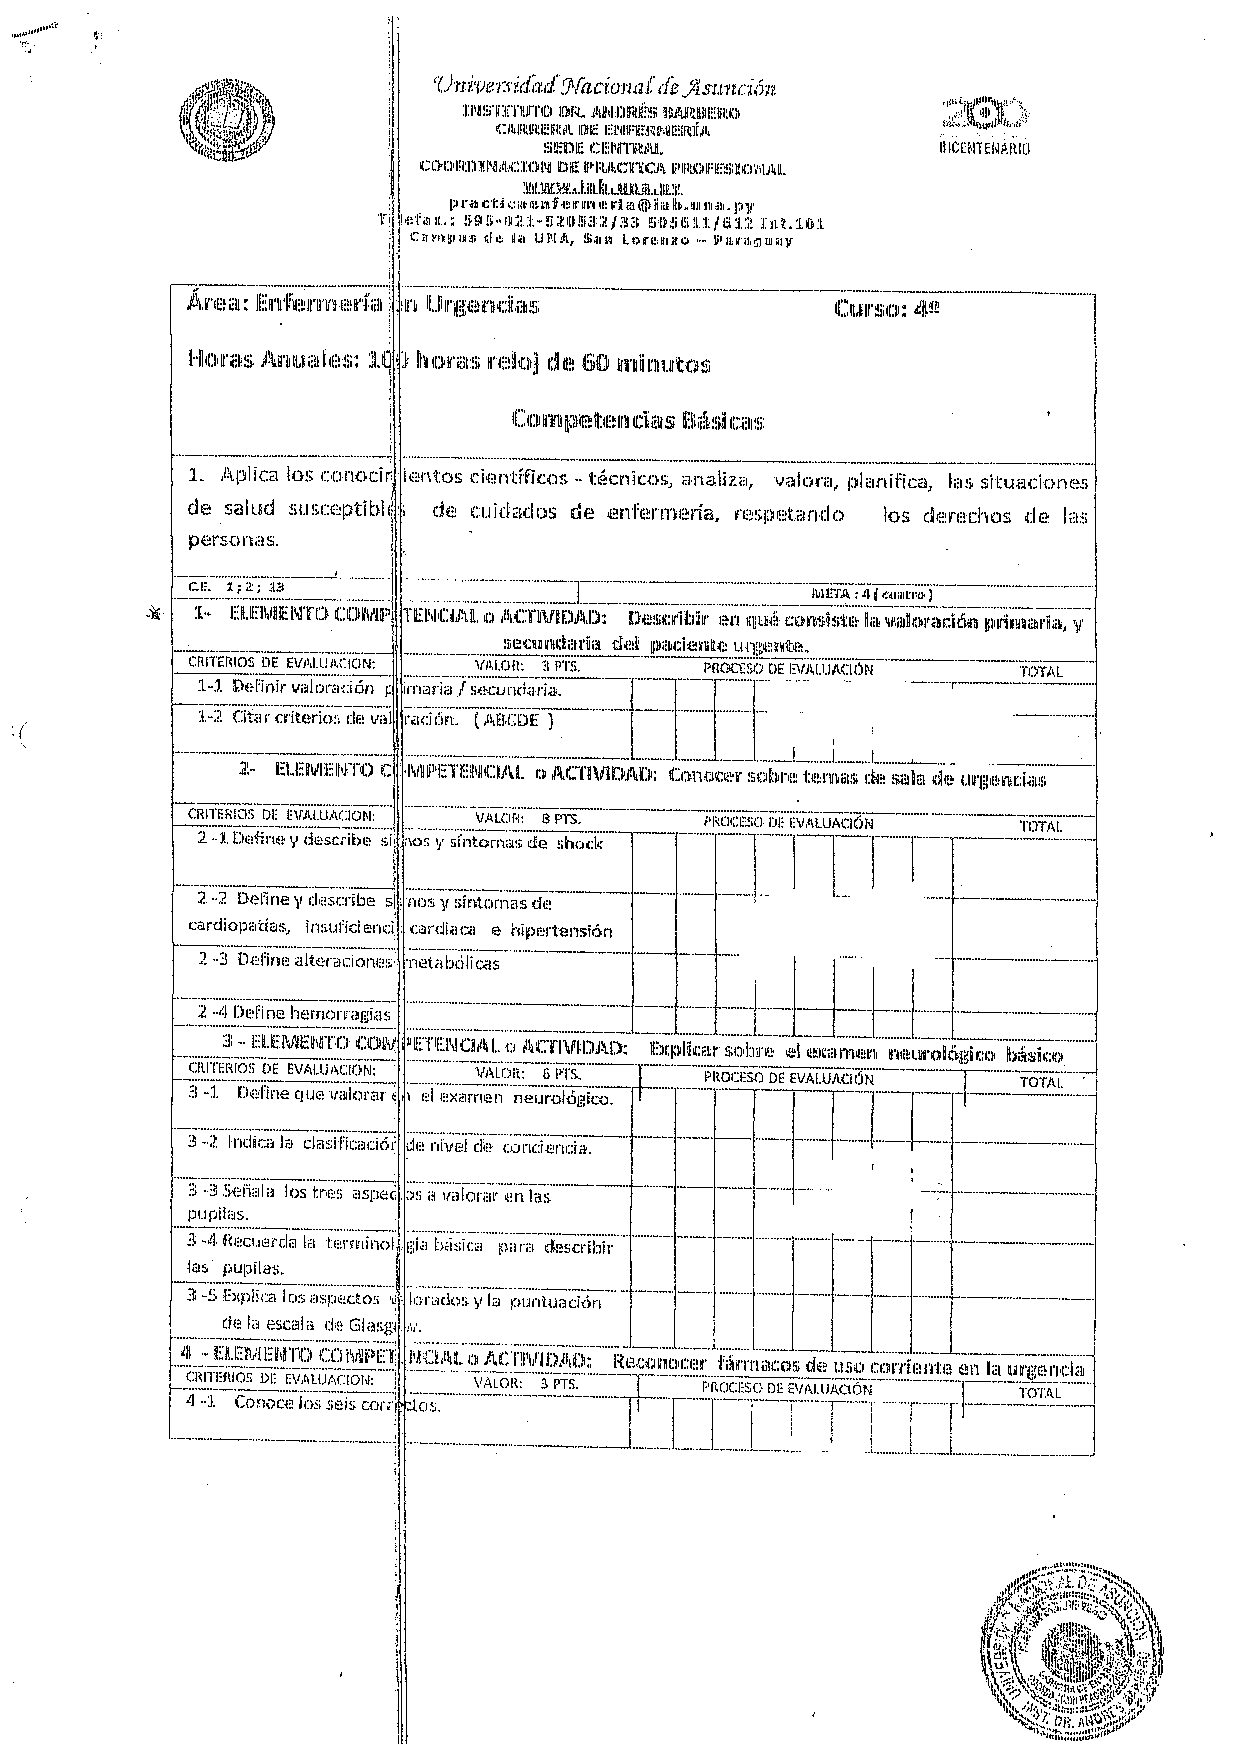
\includepdf[pages=1,scale=0.1]{anexo/documentos/planilla.pdf}
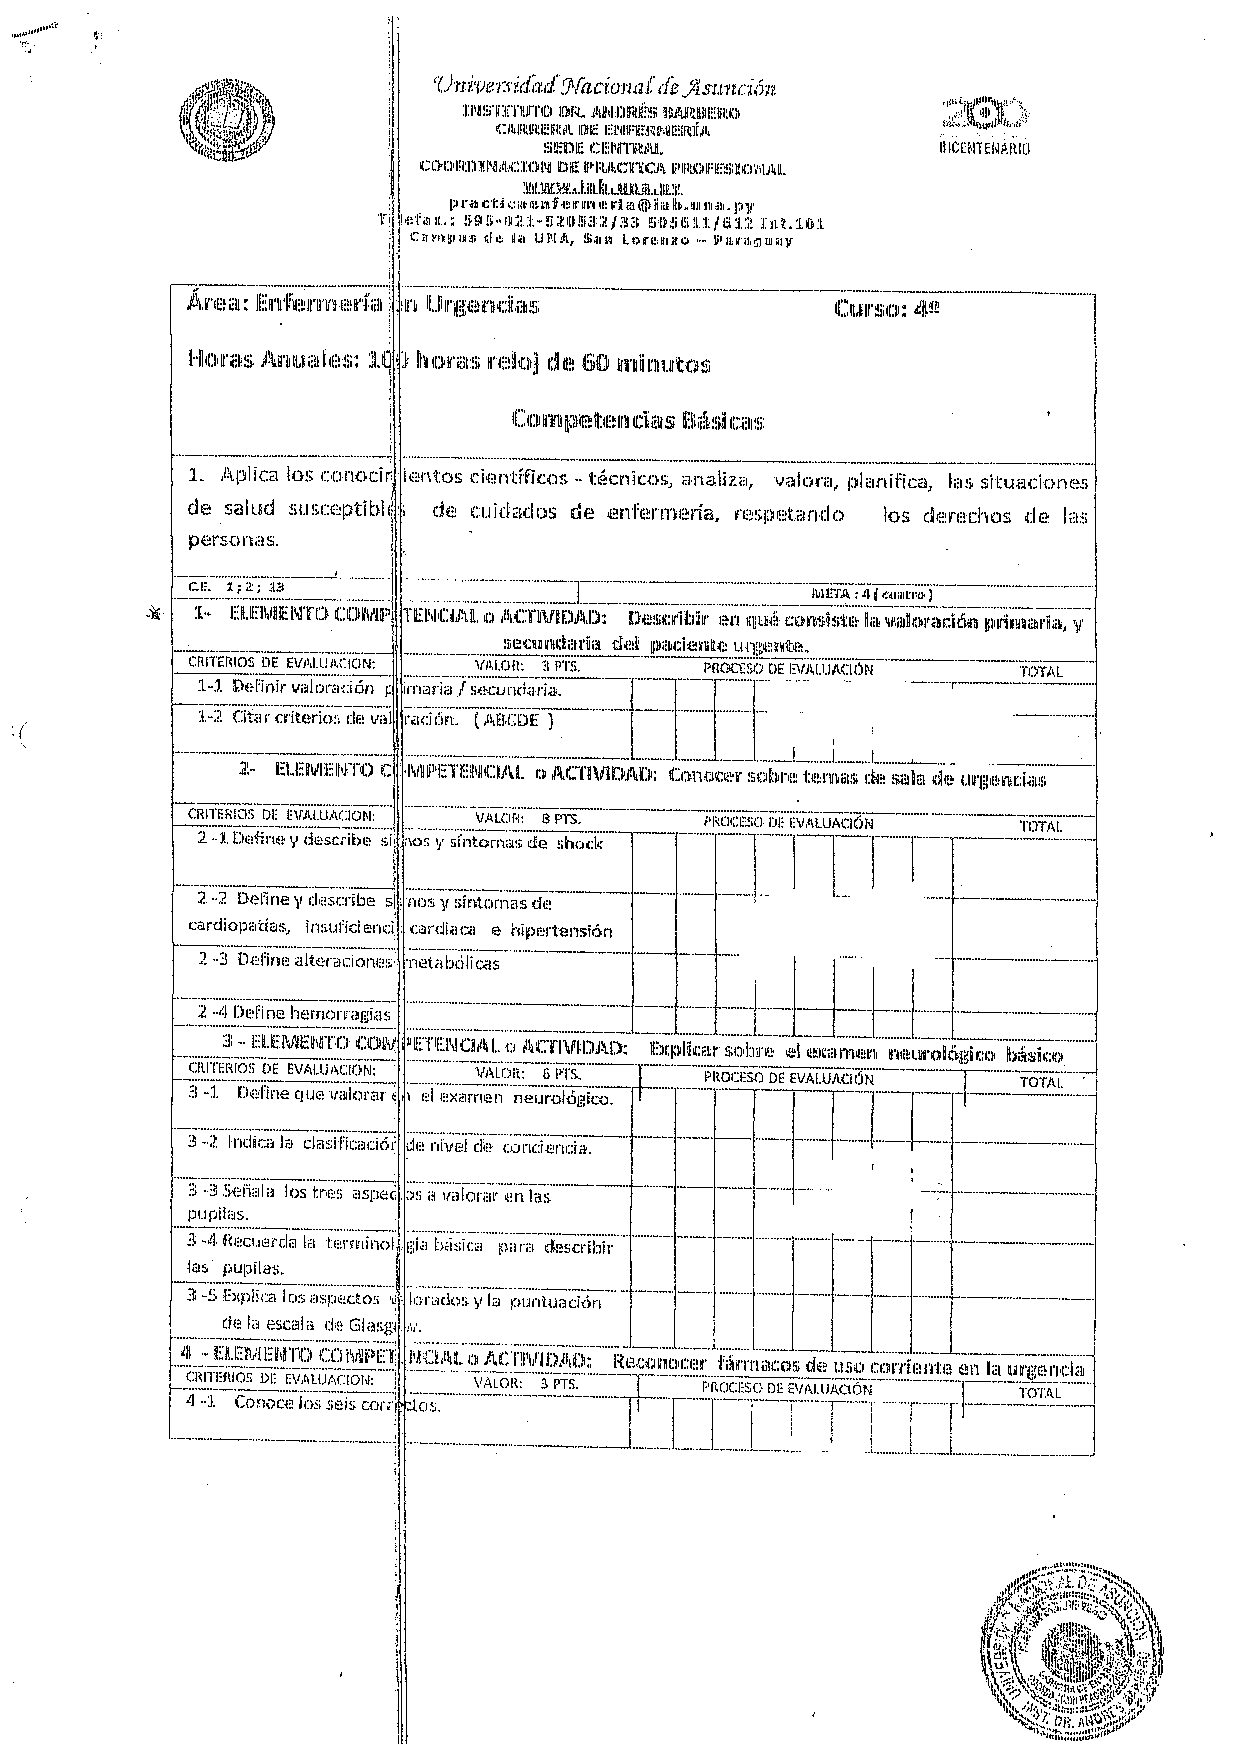
\includegraphics[scale=0.8]{anexo/documentos/planilla.pdf}
\includepdf[pages=2-4]{anexo/documentos/planilla.pdf}
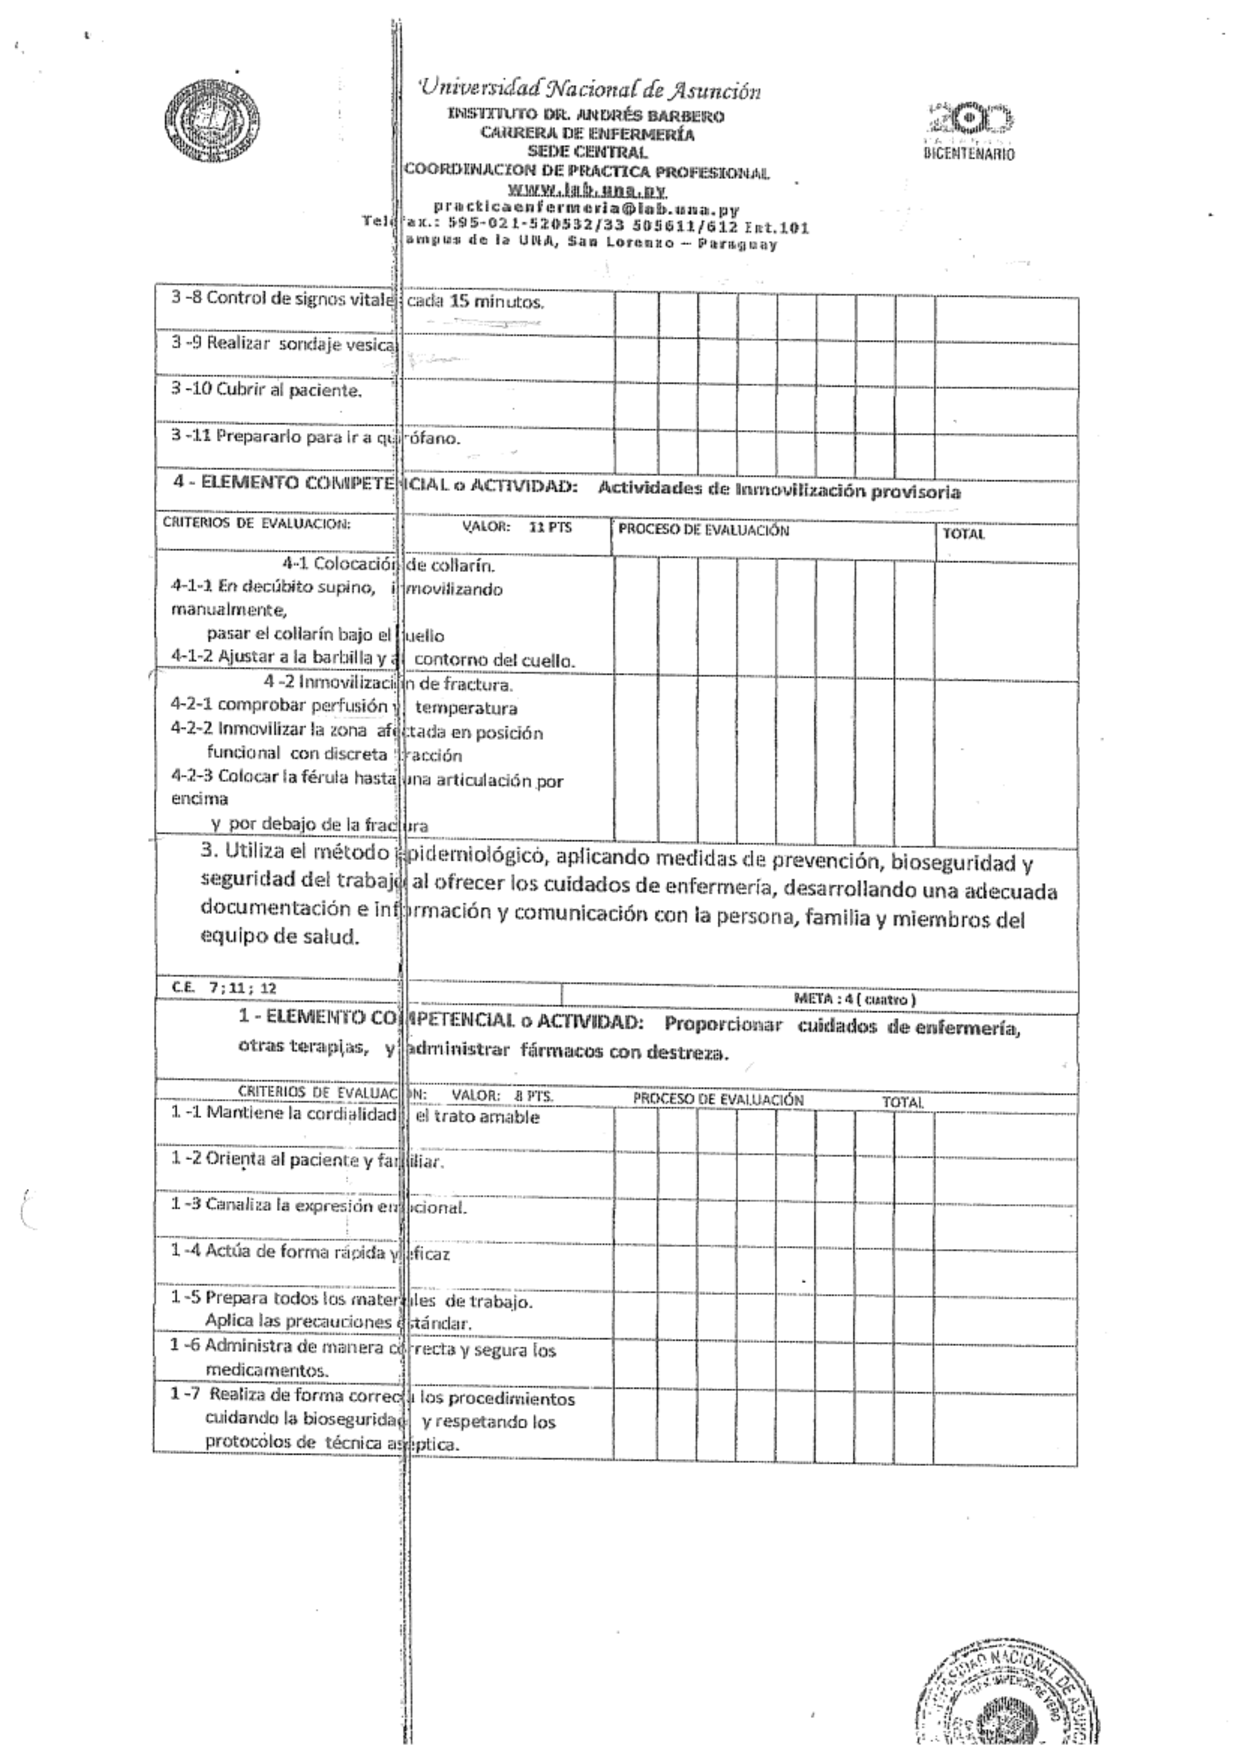
\includepdf{anexo/documentos/planilla_h_5.pdf}
\includepdf[pages=6]{anexo/documentos/planilla.pdf}

\chapter{Reuniones}

\section{Reunión \#1}\label{reuniuxf3n-1}

\begin{itemize}
\itemsep1pt\parskip0pt\parsep0pt
\item
  \textbf{Fecha} 12 de Diciembre de 2013
\item
  \textbf{Presentes} Miguela Hermosilla, Arturo Volpe, Mirta González
\item
  \textbf{Motivo} Presentación de propuesta y búsqueda de apoyo.
\item
  \textbf{Lugar} Secretaría de la carrera de Enfermería, Instituto
  Andrés Barbero
\end{itemize}

\subsection{Objetivos}\label{objetivos}

\begin{itemize}
\itemsep1pt\parskip0pt\parsep0pt
\item
  Presentar idea de tésis
\item
  Presentar la idea como un complemento a la educación actual
\item
  Investigar posibles áreas de aplicación de la idea
\item
  Investigar mecanismos de medición
\item
  Validación de la investigación previa.
\end{itemize}

\subsection{Desarrollo}\label{desarrollo}

Los interesados se presentaron en la secretaría del Instituto Andes
Barbero (IAB), para poder hablar con la directora de la carrera, la que
se presento como Mgs. Miguela Hermosilla.

Se procedió a la explicación de los objetivos y deseos por parte de los
interesados, Miguela parecía muy interesada y dispuesta a ayudar, los
puntos claves que menciono son:

\begin{itemize}
\itemsep1pt\parskip0pt\parsep0pt
\item
  No se debe enfocar como la utilización de redes Sociales, pues el IAB
  no promueve la utilización de las mismas por problemas internos.
\item
  Los alumnos del 1ero y 2do año tienen un laboratorio especializado
  donde realizan pruebas empíricas con muñecos, incluso deben pasar
  exámenes prácticos antes de poder aprobar la materia con exámenes
  \textbf{teóricos}.
\item
  En el 3er año se realiza el primer contacto con los pacientes, en el
  cual tan solo dialogan con los pacientes.
\item
  En el 4to año los alumnos acceden a quirofano, ya teniendo experiencia
  previa con los muñecos.
\item
  Existen tesis de alumnos de enfermería que hablan de la utilización de
  la tecnología para facilitar la educación.
\item
  Existen dos tipos de examenes:

  \begin{itemize}
  \itemsep1pt\parskip0pt\parsep0pt
  \item
    Prácticos, donde los alumnos prueban con muñecos y un instructor se
    encarga de medir la pericia del mismo.
  \item
    Teóricos: a través de un examen \textbf{tradicional}
  \end{itemize}
\item
  Anualmente ingresan 150 nuevos estudiantes.
\item
  Los instructores utilizan elementos distractores en sus exámenes para
  poder medir la capacidad del alumno de detectar los temas que se
  consideran más importantes
\end{itemize}

\subsection{Recomendaciones sobre la
tesis}\label{recomendaciones-sobre-la-tesis}

\begin{itemize}
\itemsep1pt\parskip0pt\parsep0pt
\item
  La población recomendada para el estudio son los estudiante de 3er/4to
  año.
\item
  La forma de medición recomendada es dotar a un grupo la tecnología y
  utilizar otros dos como grupos de control.
\item
  Cada grupo tiene un conjunto de instructores que se encargan de
  enseñar y medir la capacidad del alumno.
\item
  Posibles áreas para la simulación:

  \begin{itemize}
  \itemsep1pt\parskip0pt\parsep0pt
  \item
    Cuidados críticos (pediatria, cuidado de adultos)
  \item
    Cirugía
  \item
    Traumatologia
  \end{itemize}
\item
  Además menciono (con ayuda de colegas), las áreas que más
  inconvenientes genera en alumnos:

  \begin{itemize}
  \itemsep1pt\parskip0pt\parsep0pt
  \item
    Bio-seguridad
  \item
    Preparación de drogas
  \item
    Difusión de drogas
  \item
    Ética
  \end{itemize}
\item
  Se puede empezar el estudio en abril, donde los grupos empiezan, se
  recomienda empezar con el 2do grupo , que empieza la segunda semana de
  abril y la medición se puede realizar en Junio. Los motivos de elegir
  el segundo grupo son:

  \begin{itemize}
  \itemsep1pt\parskip0pt\parsep0pt
  \item
    El primero no esta lo suficientemente preparado.
  \item
    El tiempo del tercer grupo se solapa con exámenes y los alumnos no
    están en peores condiciones..
  \end{itemize}
\end{itemize}

\subsection{Otras recomendaciones}\label{otras-recomendaciones}

\begin{itemize}
\itemsep1pt\parskip0pt\parsep0pt
\item
  Reunirnos con los instructores de cada grupo el día 20-12-2013 para
  presentar la idea y buscar apoyo
\item
  Investigar sobre las tesis relacionadas en el área para averiguar
  cuales son las áreas que más cuestan.
\item
  Enviar un mail para solicitar más información y confirmar la reunión
  con los instructores.
\end{itemize}

\subsection{Actividades}\label{actividades}

\begin{itemize}
\itemsep1pt\parskip0pt\parsep0pt
\item
  Enviar correo para verificar disponibilidad de instructores.
\item
  Decidir sobre cual tema se realizará el trabajo y notificar para que
  Miguela pueda ayudarnos.
\end{itemize}

\clearpage
\section{Reunión \#2}\label{reuniuxf3n-2}

\begin{itemize}
\itemsep1pt\parskip0pt\parsep0pt
\item
  \textbf{Fecha} 27 de Diciembre de 2013.
\item
  \textbf{Presentes} Miguela Hermosilla, Arturo Volpe, Mirta González.
\item
  \textbf{Motivo} Presentación de ítems pre-seleccionados y evaluación
  de los mismos por la Profesora Miguela Hermosilla.
\item
  \textbf{Lugar} Secretaría de la carrera de Enfermería, Instituto
  Andrés Barbero.
\end{itemize}

\subsection{Objetivos}\label{objetivos}

\begin{itemize}
\itemsep1pt\parskip0pt\parsep0pt
\item
  Obtener la valoración de un profesional de los elementos a simular.
\item
  Investigar en que materia aprenden a mezclar medicamentos.
\item
  Obtener una reunión con los instructores, pues serán ellos quienes
  realizarán las pruebas.
\end{itemize}

\subsection{Desarrollo}\label{desarrollo}

Los interesados se presentaron en la secretaría del Instituto Andes
Barbero (IAB), para reunirse con la directora de la carrera, Mgs.
Miguela Hermosilla.

Se expusieron los items pre-seleccionados para la simulación con el fin
de que puedan ser valorados.

\subsubsection{Items presentados}\label{items-presentados}

\begin{enumerate}
\def\labelenumi{\arabic{enumi}.}
\itemsep1pt\parskip0pt\parsep0pt
\item
  Interpretación de la escala de \emph{glasgow} (Enfermería en cuidados
  intensivos, 4to año).
\item
  Reanimación cardiopulmonar básica y avanzada, distinción de los
  fármacos más utilizados (Enfermería en cuidados intensivos, 4to año).
\item
  Test de \emph{apgar} (Pediatría, 3er año).
\item
  Mezcla y administración de fármacos.
\item
  Conocimiento de las normas y medidas prácticas referentes a la
  bioseguridad.
\end{enumerate}

\textbf{Además se consultaron los siguientes puntos:}

\begin{enumerate}
\def\labelenumi{\arabic{enumi}.}
\itemsep1pt\parskip0pt\parsep0pt
\item
  Identificación de las características anatómicas y fisiológicas del
  recién nacido (Salud del niño y del adolescente, 3er año).
\item
  Demostrar destreza en la atención inmediata del recién nacido (Salud
  del niño y del adolescente, 3er año).
\end{enumerate}

\subsection{Recomendaciones del
profesional}\label{recomendaciones-del-profesional}

\begin{enumerate}
\def\labelenumi{\arabic{enumi}.}
\itemsep1pt\parskip0pt\parsep0pt
\item
  Este ítem puede ser aplicado para los alumnos del 3er o 4to año. Posee
  práctica. \textbf{Su orden de importancia es 3.}
\item
  Este ítem puede ser aplicado para los alumnos del 3er o 4to año.
  \textbf{Su orden de importancia es 1}, esto es debido a que este ítem
  tiene cero práctica en la actualidad, por que, la malla curricular no
  cuenta con temas relacionados a los primeros auxilios.
\item
  Este ítem posee prácticas, sin embargo, enfermería sólo se encargaría
  de la valoración del test. Puede ser aplicado para los alumnos del 3er
  o 4to año. \textbf{Su orden de importancia es 4}.
\item
  Este ítem no necesita pericia. Puede ser aplicado para los alumnos del
  3er año. \textbf{Su orden de importancia es 5.}
\item
  Este ítem se considera transversal, es decir, bioseguridad es
  importante en cada procedimiento. Incluye: protección, lavado de
  manos, asepsia, anti-sepsia. Es el que más práctica tiene. Puede ser
  aplicado para alumnos de 3er año. \textbf{Su orden de importancia es
  2}.
\end{enumerate}

\emph{Cabe mencionar que el orden de importancia del ítem va de 1 a 5,
siendo el 1 el indicador de mayor valor.}

\textbf{En cuanto a los demás puntos, mencionó:}

\begin{enumerate}
\def\labelenumi{\arabic{enumi}.}
\itemsep1pt\parskip0pt\parsep0pt
\item
  Este ítem está incluido en 2 (Reanimación cardiopulmonar). Puede ser
  aplicado para los alumnos del 4to año.
\item
  Este ítem depende de a que se refiera, puede referirse a:

  \begin{itemize}
  \itemsep1pt\parskip0pt\parsep0pt
  \item
    la recepción del recién nacido,
  \item
    instalación de un vía,
  \item
    instalación de sonda nasogástrica.
  \end{itemize}

  Puede ser aplicado para alumnos del 4to año. Su nivel de complejidad
  depende del punto que se tome en cuenta, así como el enfoque del
  mismo. Por ejemplo, la \texttt{recepción de un recién nacido} es un
  conocimiento importante pero con el cual se cuenta práctica, en cambio
  la \texttt{instalación de una vía} es un proceso sumamente complejo,
  que no cuenta con práctica.
\end{enumerate}

\subsection{Otras informaciones}\label{otras-informaciones}

\begin{itemize}
\itemsep1pt\parskip0pt\parsep0pt
\item
  Todas las pericias son evaluadas por un instructor.
\item
  Existen 4 estudiantes por instructor en las áreas críticas (cuidados
  intensivos, urgencias). Un área critica es aquella en la cual el
  paciente depende exclusivamente de un procedimiento externo.
\item
  Existen 10 estudiantes por instructor en las áreas no críticas.
\item
  Los instructores definen las cosas que evalúan. Cuentan con una
  planilla por alumnos para el seguimiento de las pericias (si son
  logradas o no, incluye los procedimientos).
\item
  Los instructores no están en enero.
\item
  La Sra. Miguela Hermosilla se encontrará en las instalaciones del
  Instituto Andrés Barbero del 6 al 10 de enero de 8:00 a 13:00 horas.
  Debemos reunirnos en alguna de estas fechas con ella para que nos
  pueda presentar a algún instructor que se encuentre, con el fin de que
  podamos reunirnos con él.
\end{itemize}

\subsection{Conclusiones}\label{conclusiones}

\begin{itemize}
\itemsep1pt\parskip0pt\parsep0pt
\item
  Programar una reunión con los instructores, para ello se puede
  utilizar los días que la profesora Miguela no este de vacaciones y
  pedir su ayuda como contacto directo (si existe algún instructor
  presente).
\item
  Obtener la validación de un instructor acerca de los elementos a
  simular.
\end{itemize}

\clearpage
\section{Reunión \#3}

\begin{itemize}
\itemsep1pt\parskip0pt\parsep0pt
\item
  \textbf{Fecha} 08 de Enero de 2014.
\item
  \textbf{Presentes} Prof.~Gloria Mora, Arturo Volpe, Mirta González.
\item
  \textbf{Motivo} Primer encuentro con un instructor
\item
  \textbf{Lugar} MECIP, Instituto Andrés Barbero.
\end{itemize}

\subsection{Objetivos}

Reunión con instructores para obtener su valoración acerca de los ítems
pre-seleccionados para simular, la situación actual de los alumnos de
enfermería y otras informaciones relevantes que nos pueda brindar.

\subsection{Desarrollo}

Los interesados acudieron a la Secretaría de la carrera de Enfermería en
el Instituto Andrés Barbero, donde fueron guiados por una secretaría
hasta el MECIP, donde se llevo a cabo la reunión con la profesora Gloria
Mora.

Los alumnos presentaron la propuesta y los ítems pre-seleccionados hasta
el momento.

La profesora Gloria Mora, es instructora en la materia ``Enfermería de
Urgencias'', encargada de los alumnos que atienden adultos que van al
hospital de Emergencias Médicas.

\subsubsection{Comentarios de la
profesora}

\begin{itemize}
\itemsep1pt\parskip0pt\parsep0pt
\item
  Enfermería en urgencias es una materia de cuarto curso, y se basa en
  tres competencias básicas, entre las cuales se encuentra el control de
  los signos vitales (frecuencia cardíaca, frecuencia respiratoria,
  presión arterial y temperatura).
\item
  La profesora es encargada de los alumnos durante 4 semanas, las cuales
  organiza como sigue:

  \begin{itemize}
  \itemsep1pt\parskip0pt\parsep0pt
  \item
    1 semana de prácticas en el laboratorio, si bien, según otras
    profesoras, los alumnos deben estar completamente preparados para
    las prácticas, Gloria menciona que prefiere una semana más bajo su
    supervisión para que los alumnos sepan como actuar y entiendan el
    lenguaje en el que se comunicará durante las prácticas.
  \item
    1 Semana donde la profesora guía a los alumnos en sus actividades,
    considera a esta semana como de conocimiento, exploración y
    adaptación al ambiente.
  \item
    2 Semanas durante las cuales vigila el desenvolvimiento de los
    alumnos y corrige sus actividades, al mismo tiempo que evalúa la
    pericia.
  \end{itemize}
\item
  Existe software que se utiliza para la instalación del catéter de PIC,
  de monitoreo y de soporte.
\item
  Control de los signos vitales:

  \begin{itemize}
  \itemsep1pt\parskip0pt\parsep0pt
  \item
    \textbf{Primarias}, son el control de los signos vitales, lo que
    menciono se llama el ABCDE de los signos vitales.
  \item
    \textbf{Secundarias}, la piel y daños secundarios.
  \end{itemize}
\end{itemize}

\paragraph{Evaluación}

Los alumnos del 4to curso de la materia \emph{Enfermería en Urgencias},
distribuyen la práctica como sigue:

\begin{itemize}
\itemsep1pt\parskip0pt\parsep0pt
\item
  Centro de emergencias médicas, 4 semanas, aquí es donde la profesora
  es la instructora. En este lugar atienden pacientes con accidentes y/o
  agresiones.
\item
  Urgencias en el Hospital de Clínicas, 4 semanas. En este lugar
  atienden pacientes crónicos y agudos.
\end{itemize}

Las prácticas tienen una duración de 4 horas, y son llevadas a cabo de
las 13 hasta las 17 horas (4 horas por día).

Algunas actividades que se evalúan son por ejemplo:

\begin{itemize}
\itemsep1pt\parskip0pt\parsep0pt
\item
  Posicionamiento del paciente al a hora de hacer tratamientos
  (elevación de piernas, posicionamiento de la cabeza)
\item
  Valoración del paciente (ABCDE)
\item
  Toma de sangre
\end{itemize}

Además nos entrego una copia de la hoja de evaluación, la cual es
completada por la misma para cada alumno, en la hoja se constatan las
competencias básicas y la progresión de los procedimientos en los
alumnos.

\paragraph{Tipos de alumnos}

\begin{itemize}
\itemsep1pt\parskip0pt\parsep0pt
\item
  \textbf{Desinteresado}, no muestra interés y escapa conscientemente de
  las prácticas. (\textasciitilde{}25\%)
\item
  \textbf{Introvertido}, es difícil que ayude, pero una vez que empieza
  a ayudar siempre ayuda sin problemas (\textasciitilde{}25\%)
\item
  \textbf{Extrovertidos}, ayudan sin problemas y se muestran interesados
  ante las enseñanzas, sienten que aplican la teoría
  (\textasciitilde{}50\%).
\end{itemize}

\paragraph{Tecnología}

Los alumnos deben estar familiarizados con las máquinas que sirven para
medir diferentes aspectos del estado de un paciente, y los que se
utilizan para diferentes tratamientos (como ejemplo un desfribilador).

Además, tienen permitido utilizar el celular siempre y cuando no estén
en la sala (pueden ir al baño, en la sala de descansos o cuando tienen
tiempo para comer).

\subsubsection{Otros}

Ante consultas sobre los elementos seleccionados, mostró un especial
interés por la escala de glasgow.

\clearpage
\section{Reunión \#4}

\begin{itemize}
\itemsep1pt\parskip0pt\parsep0pt
\item
  \textbf{Fecha} 08 de Mayo de 2014.
\item
  \textbf{Presentes} Prof.~Miguela Hermosilla, Arturo Volpe, Mirta
  González y Prof Matilde (laboratorio)
\item
  \textbf{Motivo} Presentación de laboratorios de prácticas
\item
  \textbf{Lugar} Secretaría general del departamento de enfermería y
  laboratorios de prácticas de estudiantes de enfermería y obstetricia.
\end{itemize}

\subsection{Objetivos}

\begin{itemize}
\itemsep1pt\parskip0pt\parsep0pt
\item
  Validación de la navegación actual de la simulación.
\item
  Exploración de los laboratorios y observación de prácticas actuales de
  los estudiantes de enfermería.
\end{itemize}

\subsection{Desarrollo}

La reunión se llevo a cabo en dos partes:

\subsubsection{Primera reunión}

La primera reunión se llevo a cabo en la secretaría de la carrera de
enfermería y cumplió con el primer objetivo, la validación de la
navegación actual.

\paragraph{Observaciones}

\begin{itemize}
\itemsep1pt\parskip0pt\parsep0pt
\item
  Es necesario un acceso directo a la parte específica del cuerpo donde
  se esta
\item
  Sala:

  \begin{itemize}
  \itemsep1pt\parskip0pt\parsep0pt
  \item
    En general, Es necesario más realismo en la escena de la simulación.
  \item
    Agregar ventanas con los colores típicos de un hospital (amarillos,
    ver fotos de la segunda reunión) realizando la práctica.
  \end{itemize}
\item
  Camilla:

  \begin{itemize}
  \itemsep1pt\parskip0pt\parsep0pt
  \item
    Eliminar las barandas de la camilla actual (mientras más sencilla la
    camilla mejor)
  \item
    La camilla debe estar más alta.
  \end{itemize}
\item
  Pacientesente:

  \begin{itemize}
  \itemsep1pt\parskip0pt\parsep0pt
  \item
    Remera mangas cortas
  \item
    Sin Anteojos
  \end{itemize}
\item
  Simulación:

  \begin{itemize}
  \itemsep1pt\parskip0pt\parsep0pt
  \item
    Tomar en cuenta la presión de la sangre
  \end{itemize}
\end{itemize}

\subsubsection{Segunda reunión}

La segunda reunión se llevo a cabo en los laboratorios de enfermaría con
la Prof Matilde, la cual es profesora de laboratorio del primer semestre
de la carrera de enfermería, se nos presentaron tres laboratorios, los
dos primeros de arquitectura similar pero diferente propósito, el
primero es un laboratorio/sala convertido en un aula donde los alumnos
observan maquetas muy detalladas del cuerpo humano y tienen sus primeras
prácticas bajo supervisión de un profesor.

La segunda sala es un laboratorio/sala que cuenta con numerosas camas
donde los alumnos práctican todo lo referente al mantenimiento adecuado
de las camas, cuenta además con maniquís que los estudiantes utilizan
para interactuar con un cuerpo, el mismo tiene una contextura similar al
de un cuerpo humano y varias partes marcadas con alertas visuales sobre
puntos de referencia, como por ejemplo donde se debe vacunar, donde se
debe realizar la reanimación, donde están las venas donde se pueden
ingresar vías, etc.

La tercera sala es un laboratorio de obstetricia, en el cual se pueden
ver varios maniquíes de bebes y partes sexuales de la mujer, todo lo
necesario para poder simular un parto.

\paragraph{Observaciones}

\begin{itemize}
\itemsep1pt\parskip0pt\parsep0pt
\item
  Los alumnos en el primer laboratorio observan, tocan y palpan los
  brazos falsos para poder saber donde están las venas importantes para
  la instalación de vías. Aquí además aprenden donde se deben ubicar
  cuando se acercan a un paciente, donde debe estar el lugar estéril
  para depositar los elementos y como preparar el equipo necesario.
\item
  El segundo laboratorio además cuenta con esterilizadores, donde los
  alumnos aprenden conceptos básicos sobre la esterilización (la teoría
  se da en otra materia), aquí más bien se manipula el esterilizador
\item
  Existen varios tipos de vías que pueden ser utilizados para una vena,
  y cada vena a su vez es capaz de aguantar ciertos tipos de vías,
  siendo las venas de las manos las que requieren vías más pequeñas. El
  único tipo de vía que no es colocado por el enfermero es la vía
  central (requiere de un anestesiologo).
\end{itemize}





\printbibliography{}


\end{document}
